\documentclass[12pt, letterpaper]{report}% "letterpaper" matches US standard paper size.
\setcounter{tocdepth}{3}
% --- PACKAGES: Each one adds a capability to LaTeX ---
% Think of packages like Python imports or C #includes.


% ---------- Page Layout ----------
\usepackage[top=1in,bottom=1in,left=1in,right=1in]{geometry} % geometry lets you set margins. 1-inch all around is standard for reports.
% ---------- Encoding & Fonts ----------
\usepackage[utf8]{inputenc}% Allows special characters (é, ü, °) to be typed directly.
\usepackage[T1]{fontenc} % Ensures proper font encoding in the output PDF. Without this, copy-pasting from the PDF can produce garbled characters.
% ---------- Graphics & Figures ----------
\usepackage{graphicx}% THE core package for inserting images.
% Usage: \includegraphics[width=0.8\textwidth]{filename.png}
\graphicspath{{figures3/}}
\usepackage{float}% Gives you the [H] placement option for figures/tables. [H] means "put it HERE, not where LaTeX thinks is best." Very useful when you need a figure right after the text that references it.
\usepackage{subcaption}% Lets you put multiple images side-by-side in a single figure environment. Example: Figure 3(a) and Figure 3(b) next to each other.
% ---------- Tables ----------
\usepackage{booktabs} % Provides \toprule, \midrule, \bottomrule for professional-looking tables.
% Rule of thumb: NEVER use vertical lines in tables. Use booktabs rules instead.
\usepackage{tabularx}% Adds the tabularx environment, which lets columns auto-expand to fill width. Great for tables that need to span the full page width.
\usepackage{multirow}% Allows cells that span multiple rows in tables.
\usepackage{longtable}% For tables that are too long to fit on one page (like a Bill of Materials).
% ---------- Math ----------
\usepackage{amsmath}% The standard package for equations. Adds align, equation*, etc.
\usepackage{amssymb}% Extra math symbols (e.g., \therefore, \because, \pm).
\usepackage{siunitx}% Proper formatting for SI units.
\sisetup{per-mode=fraction}
\sisetup{exponent-product=\cdot}
\DeclareSIUnit{\fahrenheit}{\degree F}
% Usage: \SI{100}{\celsius}, \SI{10000}{psi}, \SI{10}{\centi\meter}
% This ensures consistent unit formatting throughout the document.
% ---------- Bibliography ----------
\usepackage[numbers, sort&compress]{natbib}
% IEEE-style numeric citations: [1], [2,3], [4-7]
% "sort&compress" turns [3,1,2] into [1-3]
% ---------- Cross-Referencing & Links ----------
\usepackage[
	colorlinks=true,
	linkcolor=blue,      % Internal links (sections, figures)
	citecolor=blue,      % Citation links
	urlcolor=blue         % URL links
]{hyperref}
% Makes all references, citations, and URLs clickable in the PDF.
% Set colorlinks=false if you want boxes instead of colored text.
% ---------- Captions ----------
\usepackage[
	font=small,           % Caption text slightly smaller than body
	labelfont=bf,         % "Figure 1:" is bold
	textfont=it            % The caption description is italic
]{caption}% Makes figure/table captions look more professional.
% ---------- Headers & Footers ----------
\usepackage{fancyhdr}% Customizable headers and footers.
\pagestyle{fancy}% Activate the fancy header/footer style.
\fancyhf{}% Clear all default header/footer content.
\fancyhead[L]{\small Team 16 --- Noble Aggie Labs}% Left header: team name.
\fancyhead[R]{\small EME 185}% Right header: course number.
\fancyfoot[C]{\thepage}% Center footer: page number.
\renewcommand{\headrulewidth}{0.4pt}% Thin line under the header. Set to 0pt to remove.
% ---------- Paragraph Formatting ----------
\usepackage{parskip}% Adds space between paragraphs instead of indenting the first line. This is more common in engineering reports than academic papers.
\setlength{\parindent}{0pt}% Explicitly remove paragraph indentation (parskip should handle this, but belt-and-suspenders doesn't hurt for readability).
% ---------- Line Spacing ----------
\usepackage{setspace}
% \onehalfspacing% 1.5 line spacing is easier to read and mark up than single spacing. Change to \doublespacing if required.
\onehalfspacing
%-------- For Box diagrams
\usepackage{tikz}
\usetikzlibrary{patterns}
\usetikzlibrary{patterns,intersections}
\usetikzlibrary{arrows.meta, positioning}
\usetikzlibrary{shapes.geometric}
\usetikzlibrary{arrows.meta, shapes.geometric, shapes.misc, positioning}
\usetikzlibrary{calc}
% ---------- Appendix Support ----------
\usepackage[title,titletoc,page]{appendix} % Adds "Appendices" header and includes appendices in the Table of Contents. [title, titletoc] ensures they are labeled A, B, C
%----------- Title/Chapter formatting -----------------
\usepackage{titlesec}
% Format \chapter to look simple (no giant text, no separate page)
\usepackage{pdfpages}
% Allows you to insert entire PDF Pages (e.g., for Gantt charts, concept screening matrices) with \includepdf.
\usepackage{geometry}
%allows you to set margins and page size. 
\usepackage{mdframed}     % warning/note boxes, important equations
	\mdfsetup{linewidth=1pt}
\usepackage{enumitem}     % list formatting
\usepackage{booktabs}     % tables
\usepackage{xcolor}       % color support
\usepackage{upgreek}


\definecolor{warnred}{RGB}{180,30,30}
\definecolor{warnbg}{RGB}{255,235,235}
\definecolor{notebg}{RGB}{235,245,255}
\definecolor{noteblue}{RGB}{30,80,160}
\definecolor{ucdgold}{RGB}{207, 184, 124}
\definecolor{ucdblue}{RGB}{0, 40, 85}
\definecolor{sandiablue}{RGB}{0,  174, 214}



\newmdenv[
  linecolor=warnred, backgroundcolor=warnbg,
  linewidth=1.5pt, innerleftmargin=10pt,
  innerrightmargin=10pt, innertopmargin=8pt,
  innerbottommargin=8pt, skipabove=10pt, skipbelow=6pt
]{warningbox}

\newmdenv[
  linecolor=noteblue, backgroundcolor=notebg,
  linewidth=1pt, innerleftmargin=10pt,
  innerrightmargin=10pt, innertopmargin=8pt,
  innerbottommargin=8pt, skipabove=10pt, skipbelow=6pt
]{notebox}


\titleformat{\chapter}
 {\LARGE\bfseries}  % format
 {}                % label
 {0em}                         % sep between label and title
 {}                            % before-code
\titlespacing*{\chapter}{0pt}{20pt}{10pt}  % left, before, after


\makeatletter
\g@addto@macro\appendix{%
 \titleformat{\chapter}[block]
	{\huge\bfseries\centering}
	{\appendixname\ \thechapter}
	{0em}
	{\vspace{0.5em}\\}%
}
\makeatother

% ---------- PDF Metadata ----------
\hypersetup{
    pdftitle={Final Design Report -- Passive Temperature Compensation Device},
    pdfauthor={Team 16: Noble Aggie Labs},
    pdfsubject={EME-185A/B Senior Design, UC Davis}
}
%-----------For landscape pages----------
\usepackage{pdflscape}
\usepackage{pgfplots}
	\pgfplotsset{compat=1.18}
	\usepgfplotslibrary{fillbetween}
	\pgfmathdeclarefunction{normalpdf}{3}{%
    \pgfmathparse{1/(#3*sqrt(2*pi))*exp(-(#1-#2)^2/(2*#3^2))}%
	}
\usepackage{multirow}
\usepackage{array}      % for >{\raggedright\arraybackslash}
\usepackage{makecell}   % for \makecell
\usepackage{calc}
\usepackage{multicol}
\usepackage{wrapfig}
\usepackage{nicefrac}
\usepackage[bottom]{footmisc}

% In your preamble
\newcounter{mycounter}           % creates a counter, initialized to 0
\newcounter{sub}[mycounter]      % resets 'sub' when 'mycounter' increments
% ============================================================================
% SECTION 0.5: CUSTOM COMMANDS (Modular Helpers)
% ============================================================================
% These are reusable shortcuts. Define them once, use them everywhere.
% If a name or term changes, you only edit it in ONE place.


% --- Project-specific shortcuts ---
\newcommand{\projecttitle}{Passive Temperature Compensation Device}
\newcommand{\teamname}{Noble Aggie Labs}
\newcommand{\teamnumber}{16}
\newcommand{\sponsor}{Dr.\ Bradley Bon}
\newcommand{\organization}{Sandia National Laboratories}
\newcommand{\coursename}{EME 185}
\newcommand{\instructor}{Professor Jonathon Schofield}
\newcommand{\university}{University of California, Davis}
\newcommand{\ta}{Teaching Assistant Xiangpu Wang}
\newcommand{\duedate}{5 June 2026}
% --- Convenience commands for common terms ---
% Using these ensures consistent terminology throughout the report.
\newcommand{\device}{PTCD}
\newcommand{\degC}{^{\circ}\text{C}}    % Degree Celsius symbol, properly formatted
\newcommand{\requiredRelationship}{D_{\text{effective}} = A_1 (T_{\text{ambient}} - T_{\text{reference}}) + A_0}
\newcommand{\transferFunction}{D_{\text{eff}}=\frac{dD_{\text{eff}}}{dX} \left[\frac{dL}{dT}\frac{dX}{dL}(T-T_{\text{ref}})+X\left(T_{\text{ref}} \right) \right]}

\newcommand{\Dcold}{D_{eff}(\SI{-60}{\celsius}) = 383.5 \pm \SI{19.2}{\micro\meter}}
\newcommand{\Dhot}{D_{eff}(\SI{80}{\celsius}) = 170.2 \pm \SI{16.9}{\micro\meter}}
\newcommand{\Dref}{D_{eff}(\SI{25}{\celsius}) = 254.0 \pm \SI{12.7}{\micro\meter}}

\newcommand{\Thot}{\SI{80}{\degreeCelsius}} %Celcius
\newcommand{\Tcold}{\SI{-60}{\degreeCelsius}} %Celcius
\newcommand{\Tref}{\SI{25}{\degreeCelsius}} %Celcius
\newcommand{\specTempChange}{\SI{140}{\degreeCelsius}}

\newcommand{\specEAl}{\SI{68.95}{\giga \pascal}}
\newcommand{\specEALLV}{\SI{55}{\giga \pascal}}
\newcommand{\specEInv}{\SI{141}{\giga \pascal}}
\newcommand{\specEInc}{\SI{200}{\giga \pascal}}
\newcommand{\specActuatorCTE}{\SI{22.85}{\micro\meter\per\meter\per\celsius}} %Evaluated at 25C
\newcommand{\specMountCTE}{\SI{-30}{\micro\meter\per\meter\per\celsius}}
\newcommand{\specInvarCTE}{\SI{1.3}{\micro\meter\per\meter\per\celsius}}
\newcommand{\specInconelCTE}{\SI{13.2}{\micro\meter\per\meter\per\celsius}}
\newcommand{\specBellowsK}{\SI{75.3}{\kilo \newton \per \meter}} % 430 lb/in
\newcommand{\specBellowsHeight}{\SI{22.86}{\milli \meter}} % = Neck 1 length + Neck 2 length + Conv free diameter = 2*(0.07") + 0.76"
\newcommand{\specBellowsOD}{\SI{6.528}{\milli \meter}} % Conv OD 0.257"
\newcommand{\specBellowsID}{\SI{3.353}{\milli \meter}} % Conv ID 0.132"
\newcommand{\specBellowsSquirm}{\SI{20.68}{\mega \pascal}} % 3000 psi
\newcommand{\specBellowsBurst}{\SI{74.12}{\mega \pascal}} % 10750 psi

\newcommand{\Xhot}{\SI{480.696}{\micro \meter}}
\newcommand{\Xcold}{\SI{213.289}{\micro \meter}}
\newcommand{\specLengthChange}{\SI{267.407}{\micro \meter}}
\newcommand{\govErrorProp}{u_x = \sqrt{\frac{\pi(\sigma_x^2+\sigma_y^2)}{2}}}
\newcommand{\govActuator}{\Delta L = L_0 \Delta T \alpha}
\newcommand{\govValve}{D_{\text{eff}} = \sqrt{\frac{2}{\pi}}}
\newcommand{\specPressure}{\SI{68.95}{\mega \pascal}}%  68.94757 MPa
\newcommand{\AoneExact}{\SI{-1.524e-3}{\milli\meter\per\celsius}}
\newcommand{\Aone}{\AoneExact \pm 5\%}
\newcommand{\AzeroExact}{\SI{0.254}{\milli\meter}}
\newcommand{\Azero}{\AzeroExact \pm 5\%}
\newcommand{\imageHeight}{4in} % Default image height for figures. Adjust as needed.
\newcommand{\specCrossSectArea}{\SI{6.3e-5}{\meter \squared}}
\newcommand{\specOrigActuatorLength}{\SI{32.991}{\milli \meter}}
\newcommand{\specActDefTotal}{\SI{267}{\micro \meter}}
\newcommand{\specActDefHot}{\SI{162.4}{\micro \meter}}

% Transfer function specifications

\newcommand{\GA}{\SI{1.91}{\micro\meter\per\celsius}}
\newcommand{\GV}{\num{-0.798}}

\newcommand{\ReqA}{The device shall passively restrict gas flow according to the Required Relationship $D = A_1 \Delta T + A_0$}
\newcommand{\ReqB}{The device should remain within a \SI{10}{\centi\meter} $\times$ \SI{10}{\centi\meter} $\times$ \SI{10}{\centi\meter} Mechanical Envelope}
\newcommand{\ReqC}{The design must account for the Operational Conditions as specified.}
\newcommand{\RRfull}
{
	\begin{equation}
		\begin{aligned}
			D_{eff} &= \hat{G}_{V_0} \hat{G}_{A_0} \Delta T + D_{ref} \\
			&= \frac{dD}{dL} \frac{dL}{dT} (T_{amb} - T_{ref}) + D(T_{ref}) \\
			&= A_1 \Delta T + A_0
		\end{aligned}
	\end{equation}
}

% Valve specifications
\newcommand{\SpecVAA}{The valve subsystem shall passively control the effective orifice diameter as directly driven by the actuator at a conversion rate of $\frac{dD}{dL} = \GV$}
\newcommand{\SpecVAB}{The valve subsystem shall define the reference effective orifice diameter}
\newcommand{\SpecVABapp}{$D_{eff}(T_{ref}) = \AzeroExact$}
\newcommand{\SpecVB}{The valve subsystem shall not exceed a \SI{10}{\centi\meter} $\times$ \SI{5}{\centi\meter} $\times$ \SI{10}{\centi\meter} mechanical envelope}
\newcommand{\SpecVCA}{The housing shall withstand an internal pressure of \specPressure}
\newcommand{\SpecVCB}{Wetted components shall maintain a hermetic seal at this pressure}
\newcommand{\SpecVCC}{Wetted components shall not permit hydrogen diffusion or embrittlement}

% Actuator specifications
\newcommand{\SpecAAA}{The actuator subsystem shall passively drive the valve subsystem in response to ambient temperature at a rate of $\frac{dL}{dT} = \GA$}
\newcommand{\SpecAAB}{The actuator subsystem shall facilitate user calibration of the device}
\newcommand{\SpecAB}{The actuator subsystem shall not exceed a \SI{10}{\centi\meter} $\times$ \SI{5}{\centi\meter} $\times$ \SI{10}{\centi\meter} mechanical envelope}
\newcommand{\SpecACA}{The actuator shall minimize heat transfer within the test window}

% --- Figure insertion helper ---
% This command simplifies inserting a figure with a caption and label.
% Usage: \insertfigure{width}{filename}{caption text}{fig:label}
%
% Parameters:
%   #1 = width relative to text width (e.g., 0.8 for 80%)
%   #2 = filename (without path if images are in the same directory)
%   #3 = caption text
%   #4 = label for cross-referencing (use fig:prefix by convention)
\newcommand{\insertfigure}[4]{%
	\begin{figure}[H]
		\centering
		\includegraphics[width=#1\textwidth]{#2}
		\caption{#3}
		\label{#4}
	\end{figure}
}

% --- TODO marker for draft mode ---
% Prints a bold red "TODO" so you can easily spot incomplete sections.
\usepackage{xcolor}
\usepackage{tocloft} % For listoftodos
% --- TODO marker ---
\newlistof{todos}{tod}{List of TODO's}
\newcommand{\todo}[1]{%
    \textbf{\textcolor{red}{[TODO: #1]}}%
    \addcontentsline{tod}{todos}{\protect\numberline{\thepage}#1}%
}

% For links to spec table
\newcommand{\specref}[1]{\hyperref[tab:specs]{#1}}

\usepackage{lmodern} % DELETE BEFORE SUBMISSION; this is to help the pdf render more easily.


% ============================================================================
% BEGIN DOCUMENT
% ============================================================================

\begin{document}
\pagenumbering{roman}
\begin{titlepage}
	\thispagestyle{empty}   % No header/footer on the title page

	% --- Cover Photo: Sandia National Laboratories Aerial View ---
	\begin{center}
		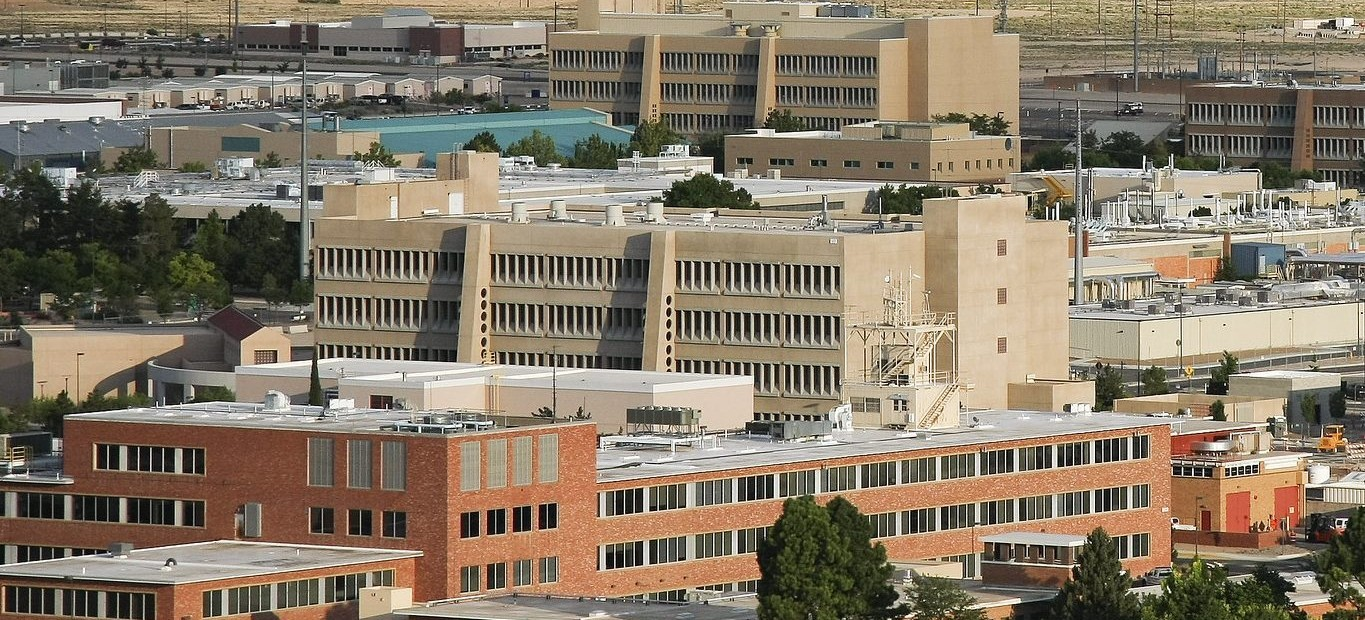
\includegraphics[width=\textwidth]{SNL4.jpg}
	\end{center}
	\vspace{0.4in}
	% --- UC Davis College of Engineering Logo ---
	\begin{center}
			
\includegraphics[width=3in]{COE.png}
	\end{center}
	\vspace{0.6in}
	% --- Project Title ---
	\begin{center}
		{\LARGE\bfseries\color{blue!70!black} \projecttitle}\\[12pt]
		{\large By the}\\[12pt]
		{\Large\bfseries \teamname}\\[24pt]
	\end{center}

	\vspace{0.4in}

	% --- Report Type ---
	\begin{center}
		{\large\bfseries FINAL DESIGN REPORT}
	\end{center}

	\vspace{0.4in}
	
	\begin{center}
		{\large SPONSORED BY \MakeUppercase{\sponsor},}\\
		{\large \MakeUppercase{\organization}}
	\end{center}

	\vfill

	% --- Submission Deadline ---
	\begin{center}
		{\large\bfseries \MakeUppercase{\duedate}}
	\end{center}

	\vspace{0.5in}
\end{titlepage}

\newpage
\thispagestyle{empty}
\vspace*{\fill}

% copyright page
\begin{center}

	{\large\bfseries Passive Temperature Compensation Device}\\[6pt]
	{\large Final Design Report}\\[24pt]

	\textcopyright\ 2026 by\\[6pt]
	Miguel Cuaycong, Jon Pizarro, Nicholas Metta,\\
	Isaiah Mathew, John Bodine, and Sam van der Veen\\[24pt]

	{\small
	
	EME 185: Mechanical Systems Design Project\\
	University of California, Davis\\[12pt]

	Advised by \instructor\ and\\
	\ta\\[24pt]

	\textit{All rights reserved. No part of this report may be reproduced}\\
	\textit{without consent from the authors, UC Davis,}\\
	\textit{or Sandia National Laboratories.}\\[24pt]

	}

\end{center}

\vspace*{\fill}

\newpage
\tableofcontents
\newpage
\listoffigures
\newpage
\listoftables

\newpage

\chapter*{\large{List of Acronyms}}

	\begin{longtable}{@{} l p{.75\textwidth} @{}}
		\toprule
		\textbf{Acronym} & \textbf{Definition} \\
		\midrule
		\endfirsthead

		\toprule
		\textbf{Acronym} & \textbf{Definition} \\
		\midrule
		\endhead

		\bottomrule
		\endfoot

		\bottomrule
		\endlastfoot

		aka			& also known as \\
		Al      & Aluminum \\
		ALLV    & ALLVAR (negative-CTE alloy) \\
		ASME    & American Society of Mechanical Engineers \\
		BOM     & Bill of Materials \\
		CAD     & Computer-Aided Design \\
		c.f.		& confer (compare) \\
		CFD			& Computational Fluid Dynamics \\
		CNC			& Computer-Numeric Control \\
		COMSOL	& Computer Solution (numerical computing software) \\
		CTE     & Coefficient of Thermal Expansion \\
		DFMEA   & Design Failure Modes and Effects Analysis \\
		DIN			& Deutsches Institut für Normung (German Standardization Institute) \\
		DOF     & Degree of Freedom \\
		EBW     & Electron Beam Welding \\
		EDM     & Electrical Discharge Machining \\
		e.g.		& exempli gratia (for example) \\
		EME     & Engineering, Mechanical (course prefix) \\
		EN			& European Norm \\
		FS      & Factor of Safety \\
		GTS			& Gas Transfer Systems (department at SNL) \\
		HEE			& Hydrogen Environmental Embrittlement \\
		ID			& Inner Diameter \\
		i.e.		& id est (that is) \\
		Inc     & Inconel 718 \\
		Inv     & Invar 36 \\
		MBD			& Multi-Body Dynamics \\
		NASA    & National Aeronautics and Space Administration \\
		NPT			& National Pipe Taper \\
		OD			& Outer Diameter \\
		PI			& Pressure Indicator \\
		PPE			& Personal Protective Equipment \\
		PTCD    & Passive Temperature Compensation Device \\
		PVD			& Physical Vapor Deposition \\
		RPN			& Risk Priority Number \\
		RR      & Required Relationship \\
		SI      & Syst\`{e}me International (International System of Units) \\
		SNL     & Sandia National Laboratories \\
		SS			& Stainless Steel \\
		TF      & Transfer Function \\
		TiCN		& Titanium Carbonitride \\
		UC Davis & University of California, Davis \\
		USA			& United States of America \\
	\end{longtable}
	% Don't worry about the error that appears here; the code should still compile

\newpage  % Start the body of the report on a fresh page

\setstretch{1.15}

\begin{abstract}

	Modern engineering constantly requires advances in technological precision and reliability.
	Sandia National Laboratories, a United States security and energy research facility, conducts many experiments that depend on submillimeter-precision flow control of high-pressure hydrogen gas.
	Their test articles are sensitive to temperature fluctuations; the flow must be adjusted to compensate for these changes.
	However, power and space constraints prohibit the use of embedded control systems, and existing passive flow control solutions do not approach the size and precision these experiments require.
	
	Sandia commissioned the Noble Aggie Labs from the University of California, Davis to design and prototype a proof-of-concept Passive Temperature Compensation Device (PTCD)
	that thermomechanically adjusts gas flow according to the ambient air temperature.
	Engineered to contain and restrict hydrogen or a noble gas up to 700 times atmospheric pressure,
	the PTCD maintains a pin-size orifice with microscopic precision. 
	It does so with a novel square-orifice valve architecture that is driven by an external, bimetallic actuator.

	This report details the design objectives, the final selected architecture, the analytical and numerical verification of system requirement satisfaction,
	and a full design package required for further iteration.

\end{abstract}

\pagenumbering{arabic}

\chapter{Introduction}
\label{chap:Fintro}

	\section{Motivation}
	\label{sec:intro:motive}

		% \begin{figure}[H]
		% 	\centering
		% 	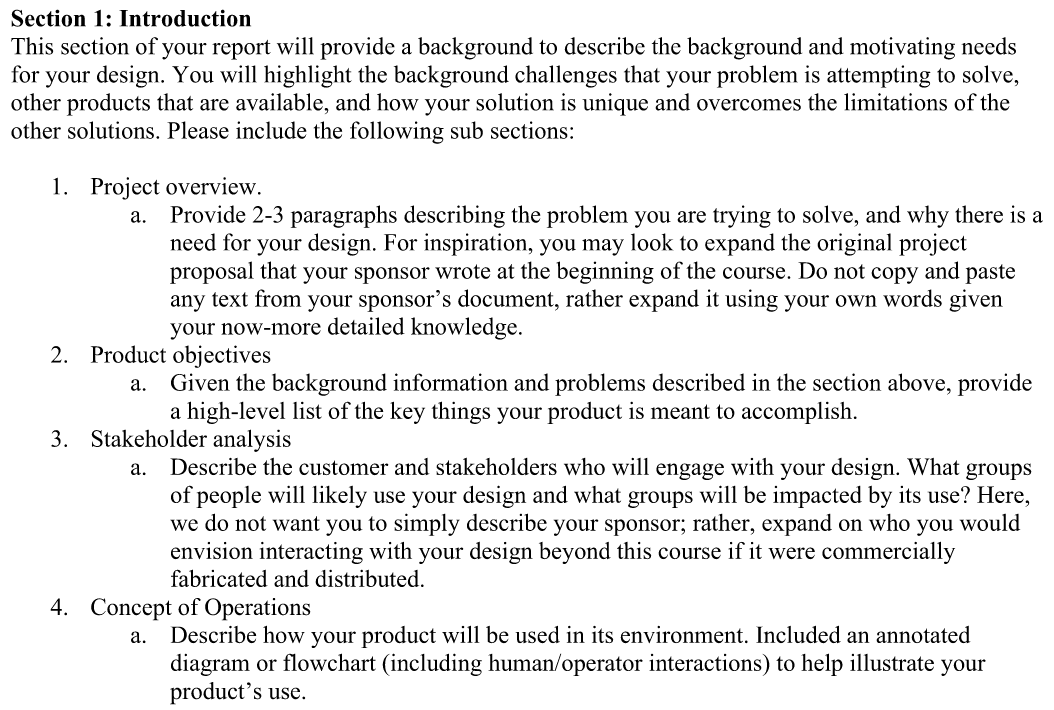
\includegraphics[width=\textwidth]{Del_introduction_requirements.png}
		% 	\caption{DELETE BEFORE SUBMISSION}
		% 	\label{fig:del_intro_req}
		% \end{figure}

		\subsection{Background}
		\label{subsec:intro:motive:background}

			National security presents ceaseless challenges.
			Engineers must deliver advanced solutions to meet the ever-increasing demand for high-performance technology.
			Sandia National Laboratories, a United States security and energy research facility in Livermore, CA, executes this mission.
			Their development of cutting-edge defense technology and scientific research protects American citizens and sojourners alike against sophisticated threats
			and pioneers advancements in energy efficiency and sustainability.
			Resolving the nation's most challenging security issues, Sandia must employ every means to maintain a competitive edge in the international theater.
			Even a small improvement in the capacity or reliability of a larger integrated system can deliver a key advantage.

			Sandia's Gas Transfer Systems team develops specialized gas flow control components and assemblies that help design, certify, and calibrate any of myriad projects undertaken at the Lab.
			Many of their developmental experiments require precision flow control of high-pressure $\text{H}_{\text{2}}$ gas.
			Downstream conditions are sensitive to environmental temperature fluctuations and must either be tightly controlled or extensively post-processed.
			Gas flow provided to the test article must be restricted by an orifice, no more than a few hundred micrometers across, that closes as the ambient air temperature rises.
			Electrically-powered valves accomplish this well.
			However, lab technicians often cannot actively control flow in these experiments due to power, personnel, or space constraints.
			They would require a fully passive thermomechanical valve, one that could control the flow of high-pressure gas across a wide temperature range with surgical precision.
			Passive temperature-compensating devices exist on the current market, but none approach the size or performance characteristics needed.
			Thermostatic actuators\cite{ref_ASHRAE_thermostatic, ref_Vernet_1938} control air-conditioning dampers or regulate the temperature of engine coolant, being especially common in the mid-20th century.
			These respond to and regulate their internal fluid temperature, rather than adjusting the internal flow in response to the ambient external conditions,
			and are designed for low-pressure, light-tolerance applications.
			Thermal louvers and thermostatic bypass valves\cite{ref_Bugby_2021, ref_Ralphs_2024, ref_Ralphs_2026} passively regulate delicate satellite equipment at the size and precision Sandia requires
			but switch on and off to compensate for the binary thermal extremes of space rather than delivering a continuous output.
			Therefore, despite this design foundation, a passive, precise valve that continuously manipulates fluid flow without responding to its conditions would prove a novel and challenging exercise.

			\subsection{Objectives}
			\label{subsec:intro:motive:objectives}

				Thus it is that Sandia National Labs (SNL, aka the ``sponsor'') employed the Noble Aggie Labs, a mechanical design team at the University of California in Davis and the authors of this paper,
				to develop a high-pressure, hydrogen-compatible, Passive Temperature Compensation Device (\device) that precisely controls a submillimeter orifice in response to a wide ambient temperature range
				while remaining agnostic to its internal flow conditions and that can be easily integrated into existing experiments.
				Engineers at SNL quantified exact system requirements according to their needs and will further iterative development upon receipt of the design package outlined in this report,
				which presents a fully-functional computational prototype of the PTCD that accomplishes the following objectives:

				\begin{itemize}
					\item Restrict the provided flow of gas, at a pressure of up to \SI{69}{\mega\pascal} (690 atmospheres), with an orifice smaller than the tip of a ballpoint pen.
					\item Adjust the orifice size in response to the ambient external temperature without external power, input, or regard to internal flow conditions, with an effective-diameter tolerance of up to \SI{20}{\micro\meter}\footnote{No more than the width of a human hair\cite{ref_NIH}.}.
					\item Do so without depending on external power, using active control, or exceeding a volume of $(\SI{10}{\centi\meter})^3$.
				\end{itemize}
			
		\subsection{Potential stakeholders}
		\label{subsec:intro:motive:stakeholders}

			The \device\ provides robust fix-and-forget control of experimental parameters.
			These experiments are run by the Gas Transfer Systems team to develop flow control components and assemblies,
			which are in turn used by Sandia in the development, certification, and calibration of various defense technologies they produce
			(depicted in Figure~\ref{fig:app_SNL} in the Appendix).
			The \device\ would primarily ease the job of test engineers and technicians, who, after one-time assembly, could leave the control system unattended indefinitely.
			Secondarily, the \device\ eliminates the need for post-process data adjustment by research engineers due to changing experimental conditions.

			This proof-of-concept design would also pave the way for similar devices with equally precise control outputs but slightly different output values, tuned as necessary for the given experiment.
			Research engineers at SNL with access to such capabilities could quickly design a new configuration of the device more suitable for the particulars of their research.

			The valve could similarly be custom-ordered by external organizations once the reconfiguration process is streamlined.
			Companies in the aerospace, military, or gas handling and processing industry may have a use for a high-pressure, high-precision, input-free valve.
			The radical nature of the \device\ makes development of similar devices easy by comparison. 

		\subsection{Concept of Operations}
		\label{subsec:intro:motive:Ops}

			Operation of this valve consists primarily of assembly and installation. After the device is assembled at Sandia's machine shop, the manufacturers thread the valve into a stream of low-pressure, room-temperature air.
			Precisely measuring the upstream and downstream gas pressure and external air temperature, they adjust a calibration screw until it reaches its reference setpoint.

			As a test engineer sets up his experimental apparatus, he inserts the calibrated valve at any orientation into gas flow upstream of the experiment by threading the existing pipe into corresponding holes in the valve.
			No further attention is needed until the device malfunctions at the end of its lifetime, at which point the entire device must be replaced.
			The chief advantage of this device is its passive nature; if it works correctly, test engineers can ignore the entire control system during its lifetime or until they need to change the experiment.
			As represented in Figure~\ref{fig:conceptual}, the \device\ converts high-pressure gas flow into controlled, low-pressure gas flow by responding only to changes in temperature.

			\begin{figure}[H]
				\centering
				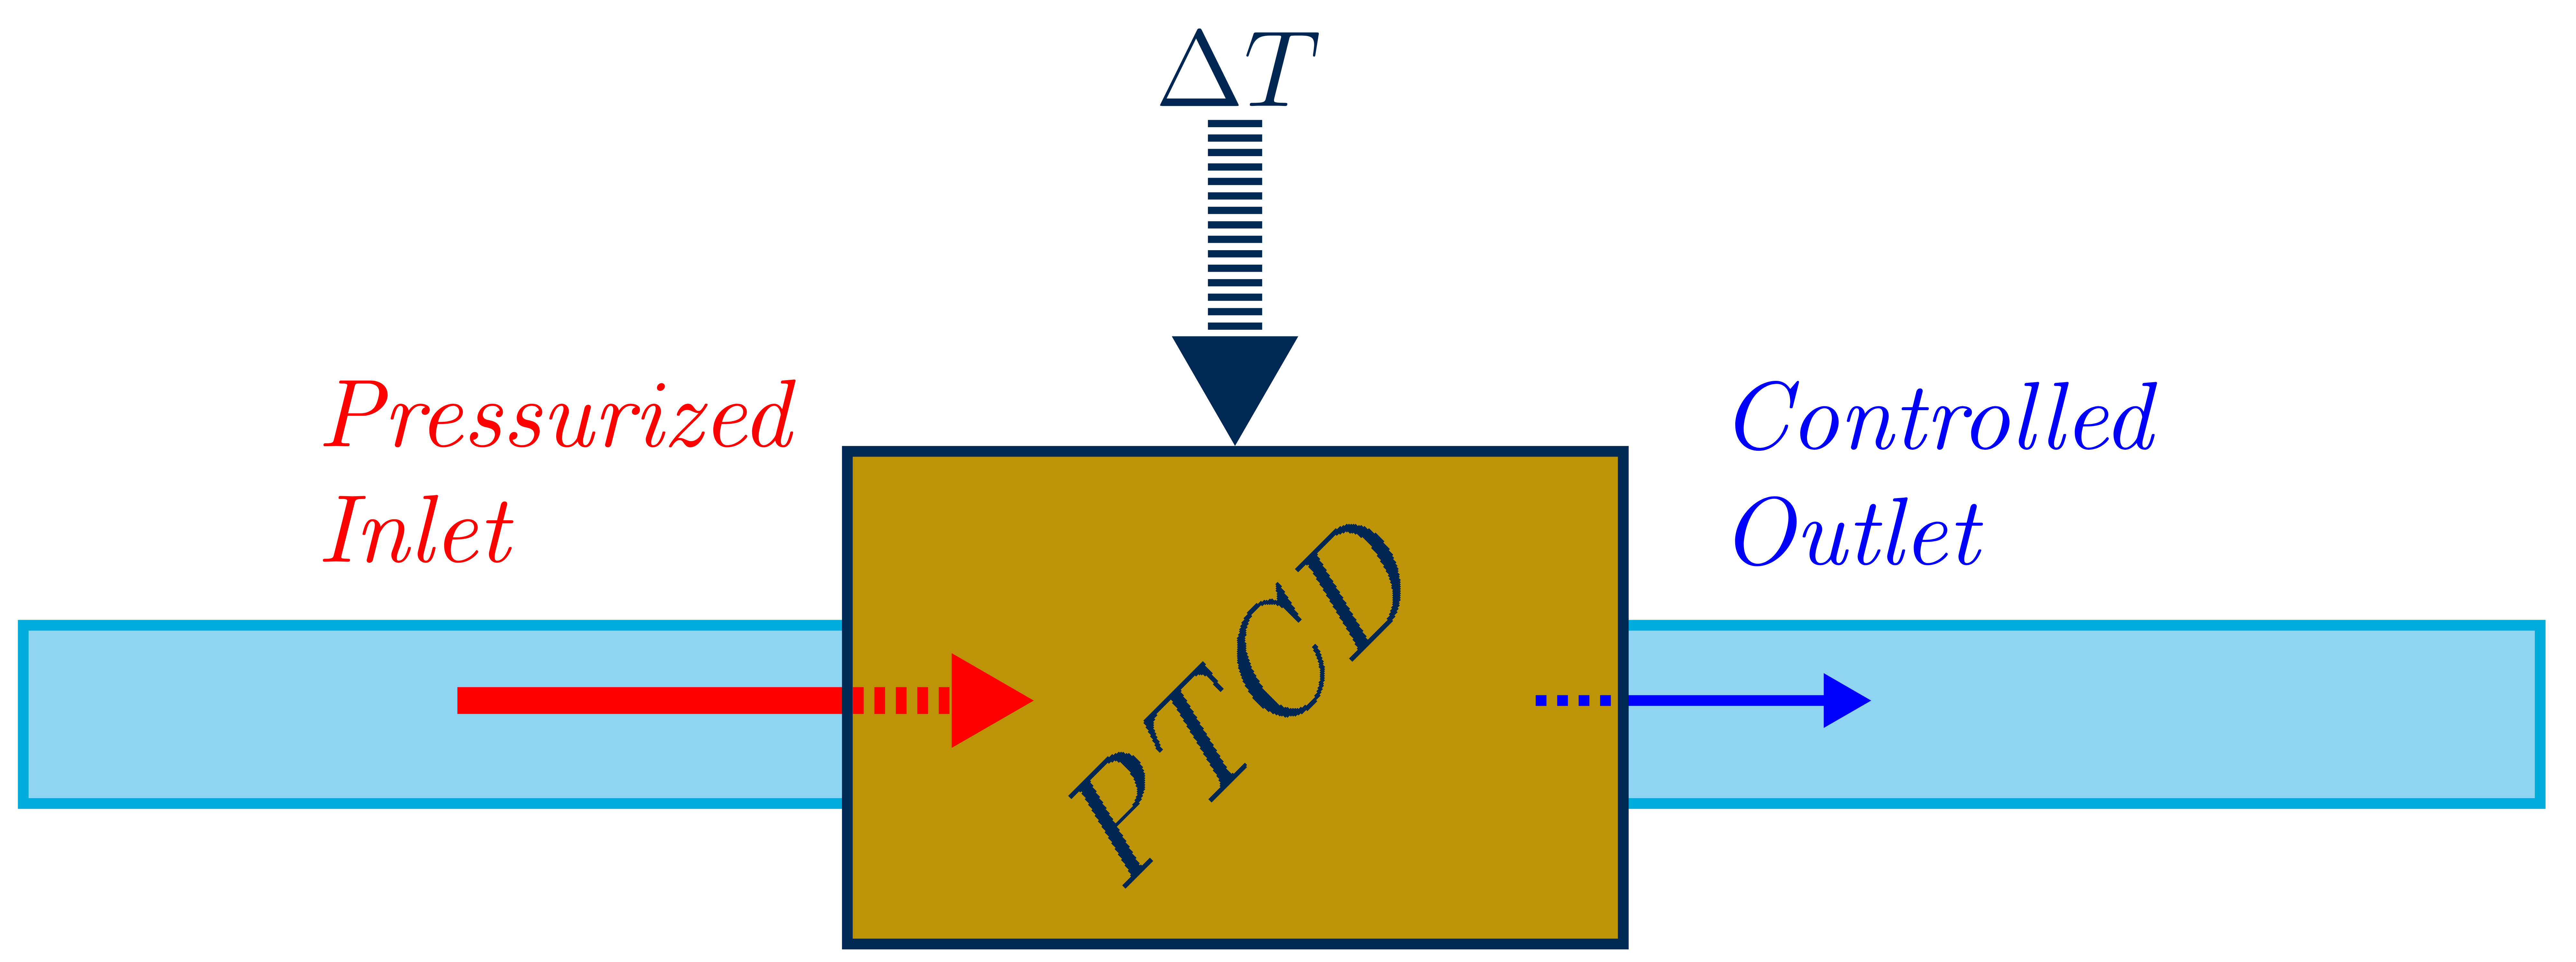
\includegraphics[height=1.8in]{conceptual.png}
				\caption{Conceptual diagram of the \device}
				\label{fig:conceptual}
			\end{figure}

				\subsubsection*{Roadmap}
				\label{subsubsec:roadmap}

					This Design Report presents the first complete iteration of the PTCD and provides a full design package required for further development.
					The following sections outline the system requirements and specifications, illustrate and justify the final system architecture, and provide several parallel verifications of system requirement satisfaction.
					Useful calculations, images, and data sheets, manufacturing and operation guides, and the complete engineering drawing package and bill of materials are appended.

	\section{System Requirements}
	\label{sec:intro:req}

		% \begin{figure}[H]
		% 	\centering
		% 	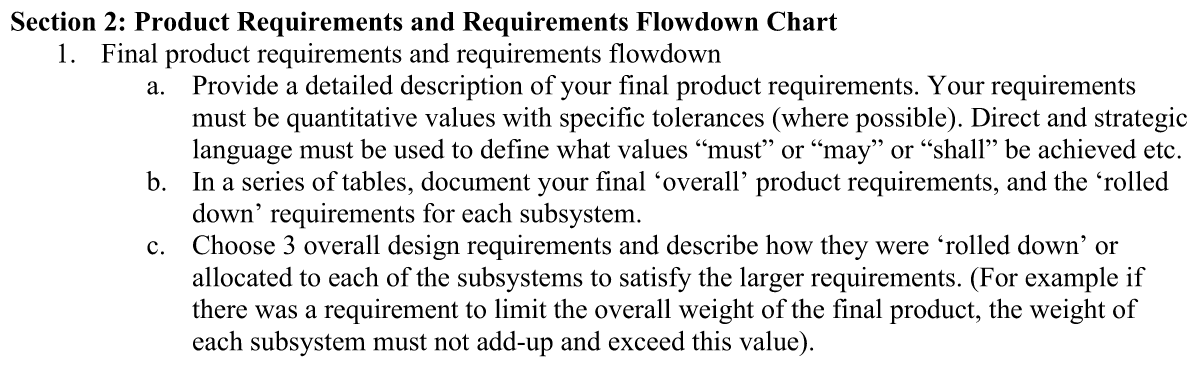
\includegraphics[width=\textwidth]{Del_requirements_requirements.png}
		% 	\caption{DELETE BEFORE SUBMISSION}
		% 	\label{fig:del_req_req}
		% \end{figure}

		\begin{multicols}{2}
			\begin{figure}[H]
				\centering
				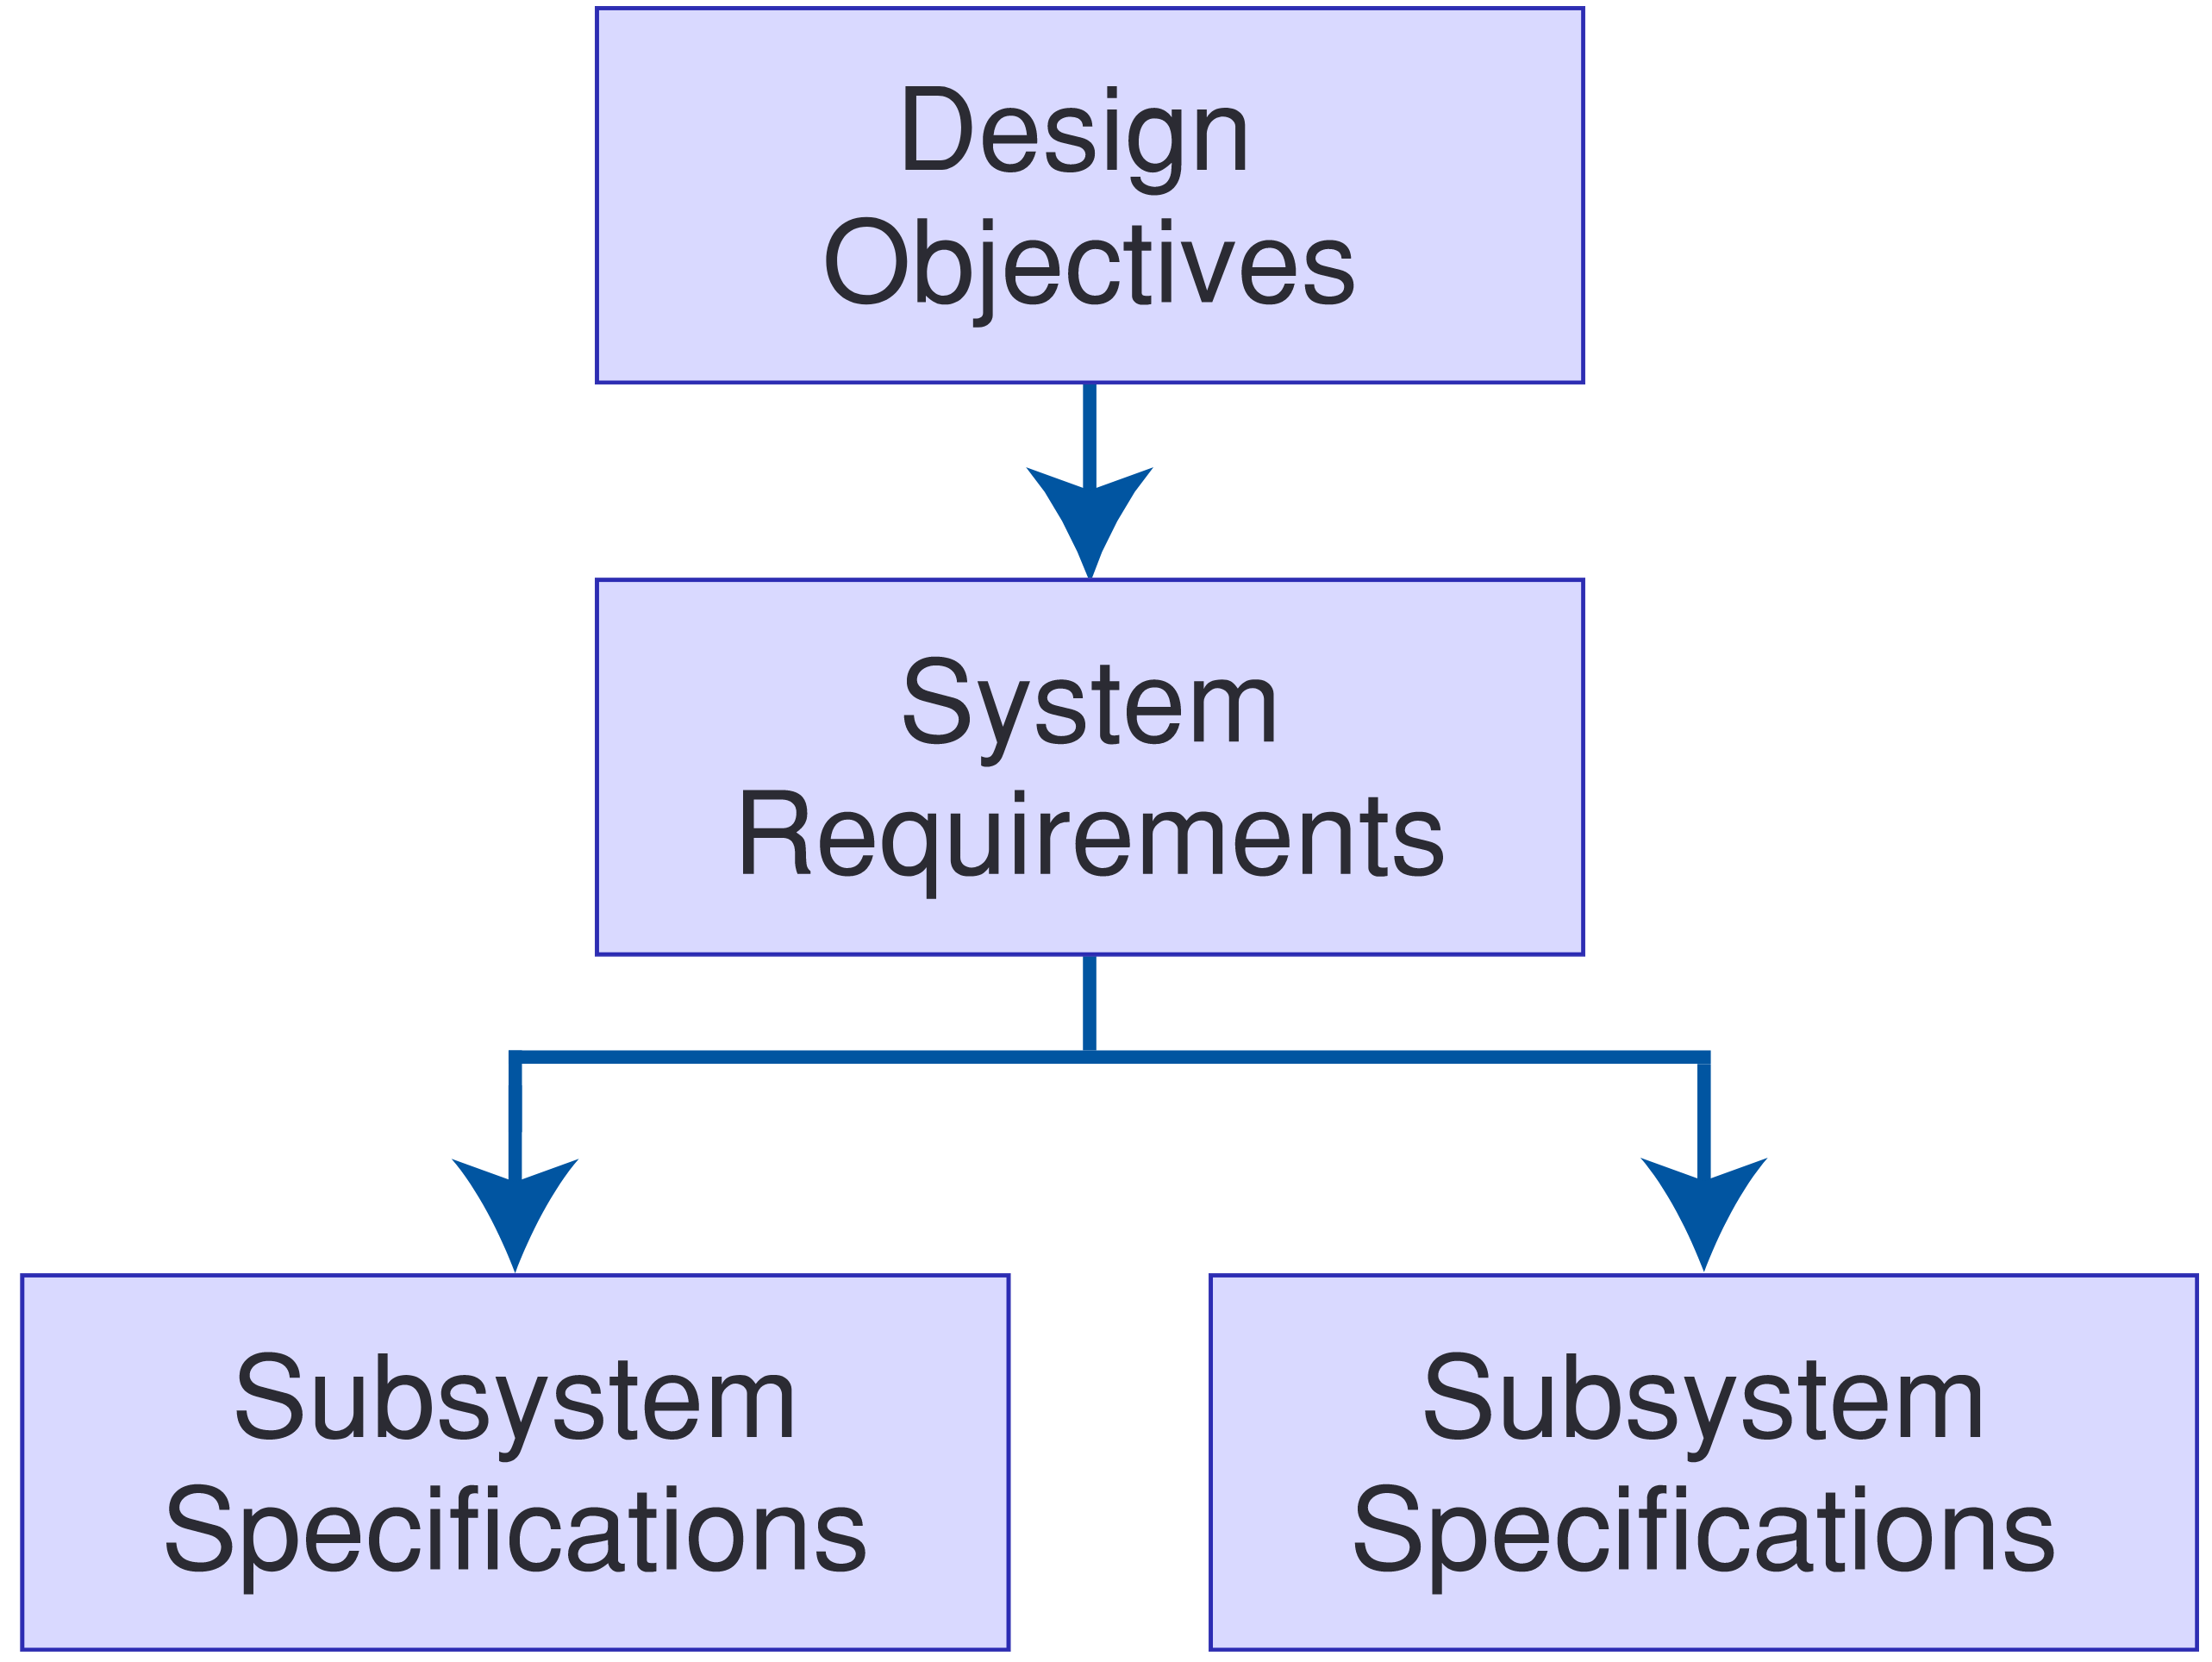
\includegraphics[width=.4\textwidth]{NASA_req.png}
				\caption{System requirement definition flowdown}
				\label{fig:NASA_req}
			\end{figure}

			\newcolumn

			NASA's Systems Engineering Handbook lays out guidelines for system requirement definition\cite{ref_NASA_specs_guide}.
			Typically, a technical systems design project involves two preliminary tasks: definition of functional and performance system requirements that satisfy the client's stated objectives
			and rolldown of those system-level requirements into subsystem specifications. This is shown in Figure~\ref{fig:NASA_req}.
		\end{multicols}

		Sandia defined three system requirements prior to commission:

		\begin{enumerate}
			\item The device shall passively restrict gas flow according to the following Required Relationship between its effective orifice diameter and the ambient air temperature:
			
				\begin{equation}
					\requiredRelationship
					\label{eq:required_relationship}
				\end{equation}

				Where:
				\[
				\begin{array}{@{} l @{\qquad} l @{}}
					T_{\text{reference}} \text{ (aka } T_{ref}\text{)} = \Tref
						& A_1 = \Aone \\[4pt]
					T_{\text{ambient}}\ \in\ [\Tcold,\Thot]\
						& A_0 = \Azero
				\end{array}
				\]

			\item The device should remain within a Mechanical Envelope of $\SI{10}{\centi\meter} \times \SI{10}{\centi\meter} \times \SI{10}{\centi\meter}$
			
			\item The device will do so under the following Operational Conditions:
			
				\begin{enumerate}
					\item \label{cond:P} 		The operating gas pressure $P$ will lie within the range $\SI{689.5}{\kilo\pascal} \leq P \leq \specPressure$
					\item \label{cond:dP} 	The gas pressure differential $\Delta P$ will lie within the range $\SI{68.95}{\kilo\pascal} \leq \Delta P \leq \specPressure$.
					\item \label{cond:dT} 	The provided gas will be up to \SI{20}{\degreeCelsius} hotter than the ambient air.
					\item \label{cond:gas} 	The gas will be a noble gas or hydrogen.
					\item \label{cond:pipe} The gas will be supplied by a stainless steel pipe of diameter \SIrange{1.524}{25.4}{\milli\meter}.
					\item \label{cond:fix} 	The ambient temperature will remain fixed during operation.
					\item \label{cond:test} The device will be tested by Sandia to validate required compliance, both without gas flow and for up to 60 seconds with gas flow.
				\end{enumerate}

		\end{enumerate}
		
		Note the difference between the obligation keywords, ``shall'' and ``should'', of the first two requirements.
		As laid out by NASA's handbook, the former indicates a strict requirement, whereas the latter gives a goal while allowing for violation in favor of a higher-priority trade-off.
		In this case, the Mechanical Envelope, the total volume that the device is allowed to occupy at all times, may (and will) be violated within reason for the sake of satisfaction of the Required Relationship.
		The Operational Conditions, denoted with the keyword ``will'', simply define the environmental parameters that must be designed for.

		The Required Relationship in equation~\eqref{eq:required_relationship} is the key objective of the PTCD. It requires that a small orifice diameter be controlled with extreme precision.
		As derived in Appendix~\ref{app:calcs:errorProp}, the effective orifice diameter ($D_{eff}$, the diameter of a circle of equivalent area)
		must linearly follow the ambient external air temperature ($T_{amb}$) and intersect the following points at each temperature boundary and at $T_{ref}$:

		\begin{align}
			\Dcold \label{eq:coldBoundary} \\
			\Dref \label{eq:DTref} \\
			\Dhot \label{eq:hotBoundary}
		\end{align}

		These are equivalent to the surface temperature of Antarctica in winter, room temperature, and the temperature of a running engine, respectively.
		This small valve must thermomechanically control a sub-millimeter orifice to a micron-scale tolerance, maintaining a linear output across a wide temperature range under extreme pressures.
		

	\section{Subsystem Specifications}
	\label{sec:intro:specs}
		
		Passive, temperature-responsive gas flow control requires two coupled subsystems:

		\begin{itemize}
			\item A valve to restrict the flow
			\item An actuator to drive the valve's movement as driven by temperature
		\end{itemize}

		The valve assembly must contain and restrict the gas flow.
		This requires a housing that can be threaded to two gas pipes, an internal variable-size orifice, and a hermetically-sealed valve stem to connect to the actuator.
		
		The actuator assembly must influence the valve from the outside so it responds to the ambient air temperature.
		Thus, it should be externally mounted to the valve and drive its motion via the valve stem (Figure~\ref{fig:subsystems_conceptual}).

		\vspace{-1em}
		\begin{figure}[h]
			\centering
			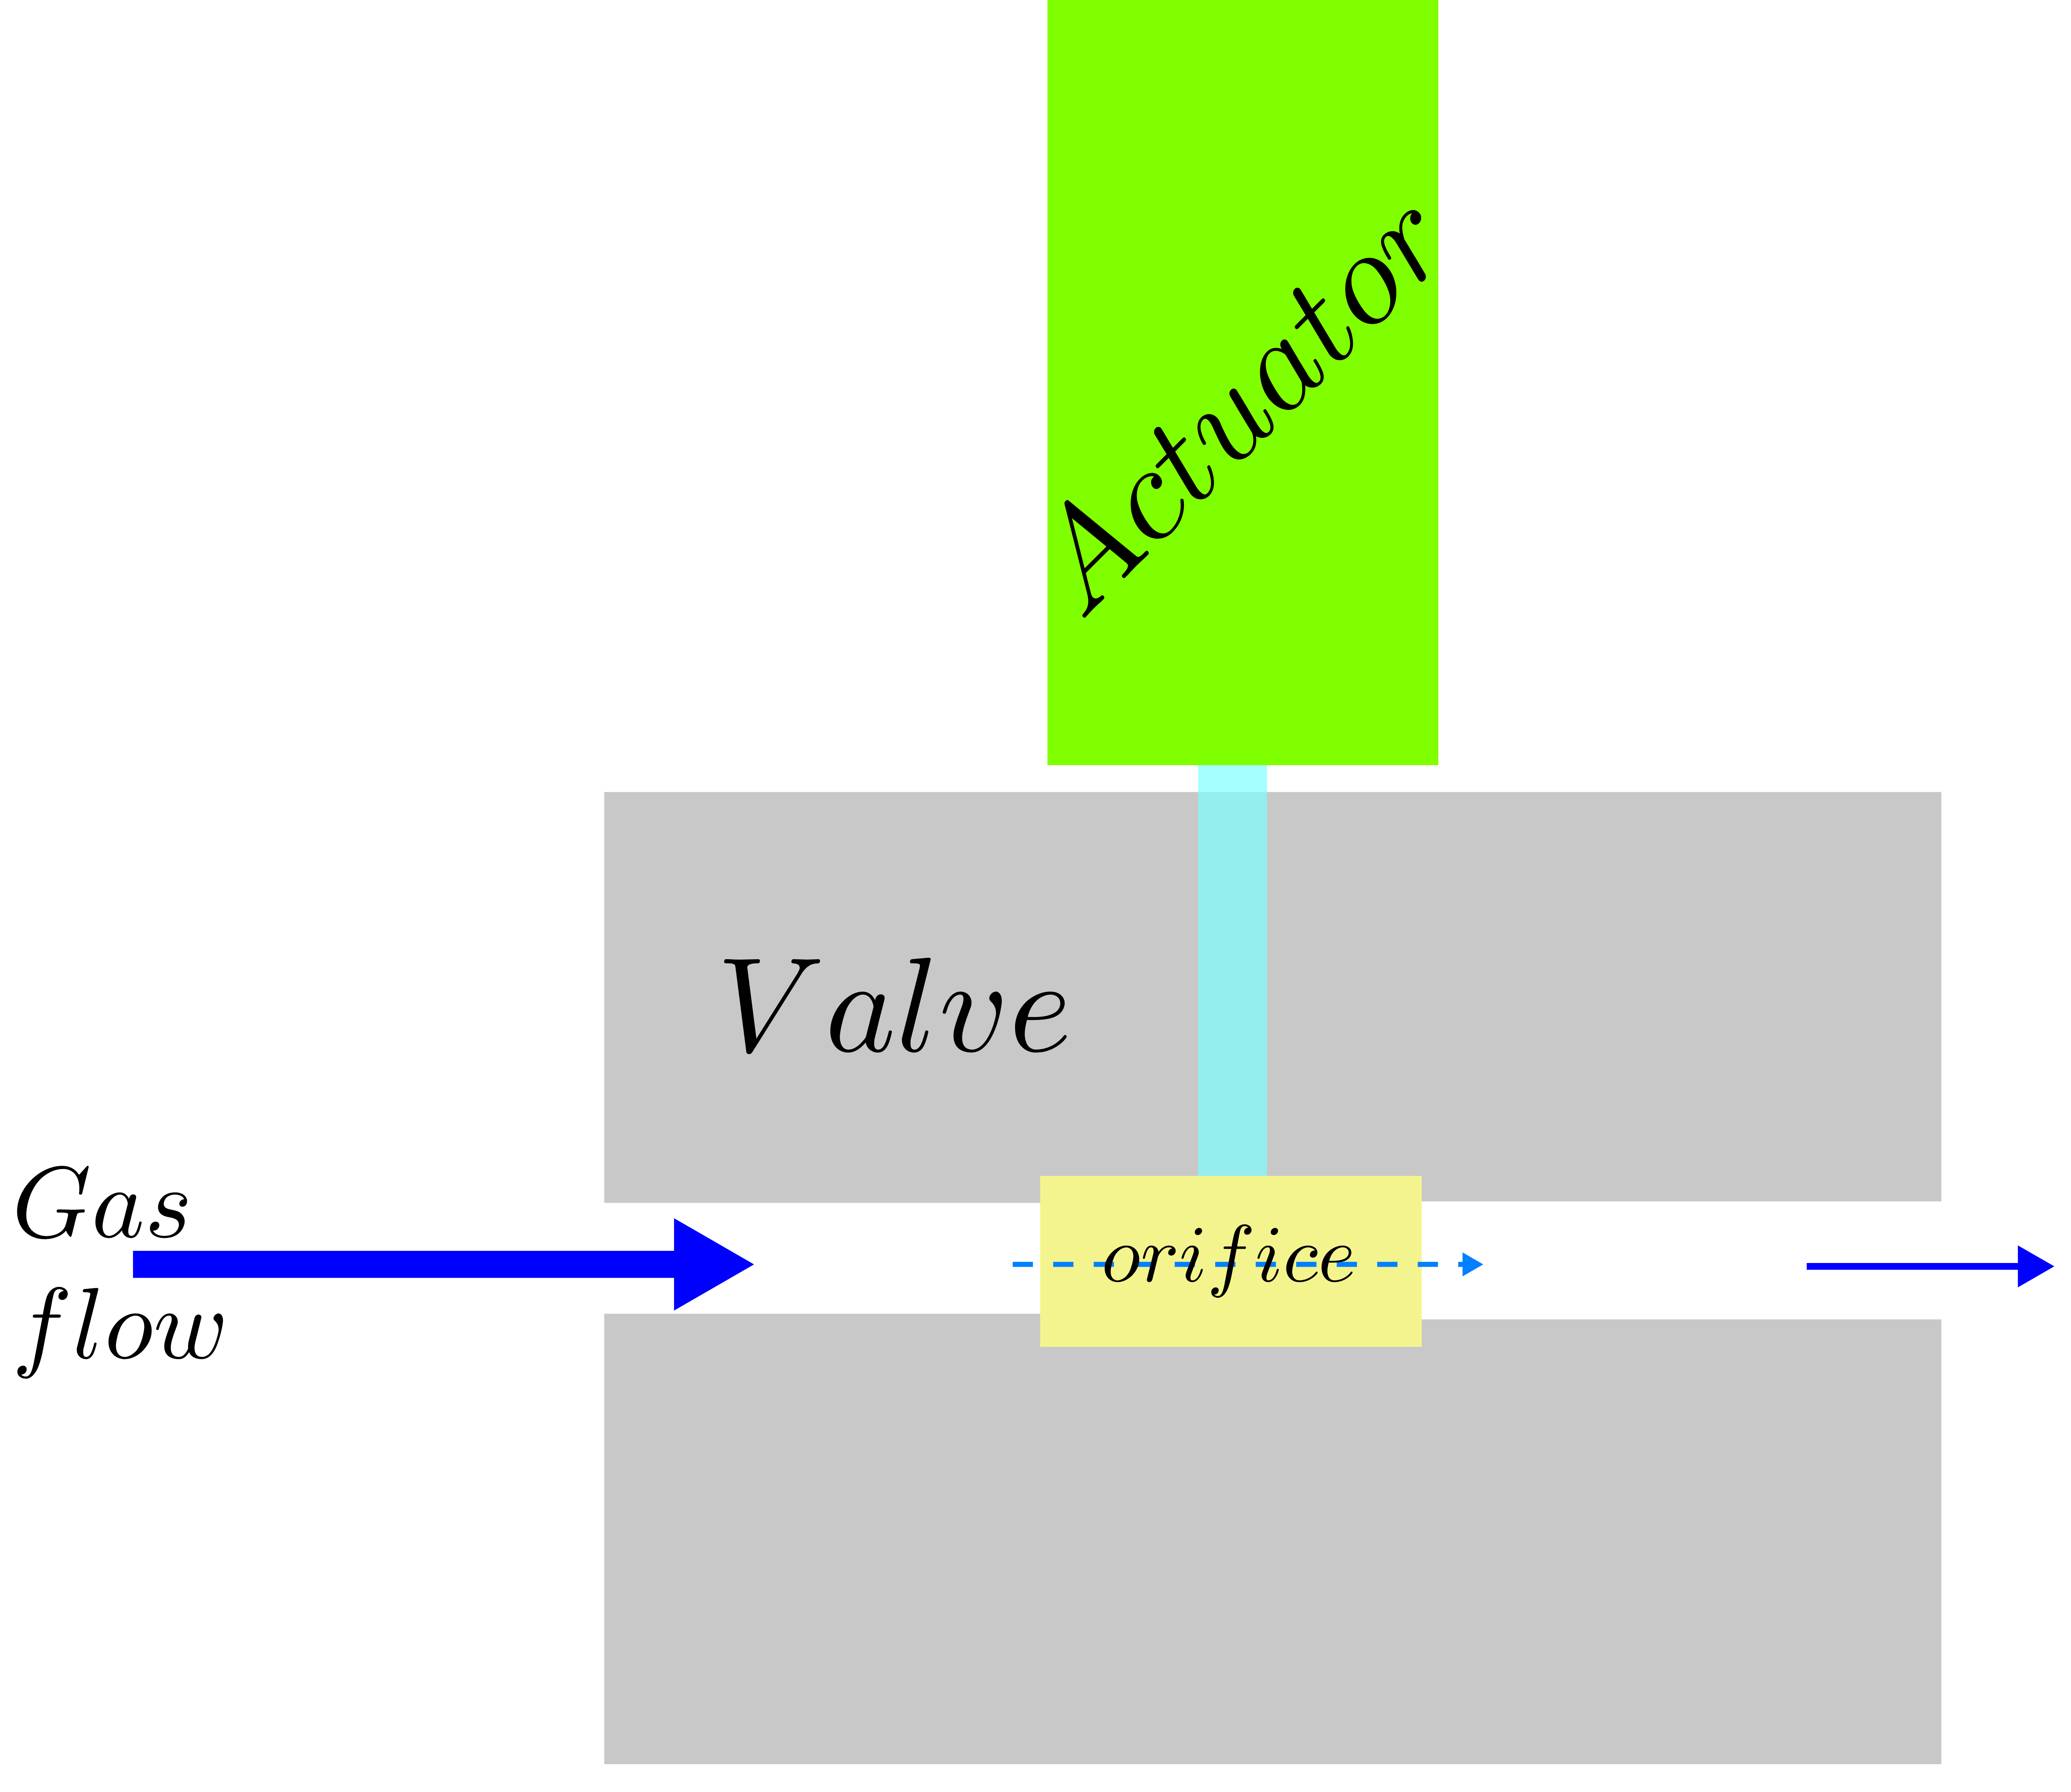
\includegraphics[width=.5\textwidth]{subsystems_conceptual.png}
			\caption{Subsystem conceptual diagram}
			\label{fig:subsystems_conceptual}
		\end{figure}

		As depicted in Figure~\ref{fig:NASA_req}, this division of subsystems allows for an informative rolldown of the above system requirements
		into several functional subsystem specifications that, if met, guarantee system requirement satisfaction.
		Because subsystem errors are not cumulative, the required tolerance cannot be properly divided between the subsystems;
		this will remain quantified at a 
		Due to the coupled nature of these subsystems, useful tolerances cannot be divided by subsystem;
		thus, these specifications will remain nominal, and quantitative performance specifications will remain at a system level.

		\subsection{Required Relationship rolldown}
		\label{subsec:intro:specs:RR}

			The Required Relationship is best understood as a passive system transfer function, commonly used in the field of control theory\cite{ref_Nise},
			represented by a simple open-loop diagram as in Figure~\ref{fig:TF_gen}.
			Systems are represented by blocks, while ``signals'', or input and output values, are represented by arrows.
			The System Transfer Function $\hat{G}_{sys}$ mathematically represents the physical input-output translation of the passive control system,
			indicating the effective diameter produced for any given input temperature. 
			Notice the absence of a feedback loop.
			Rather than depending on an active controller to sense and tune the system's output, this device must be precisely dimensioned to achieve the desired output without real-time adjustment.

			% \vspace{1em}
			\begin{figure}[H]
				\centering
				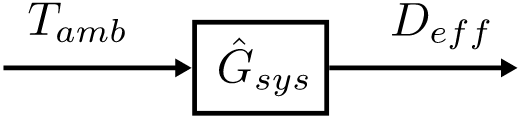
\includegraphics[width=.4\textwidth]{TF_gen.png}
				\caption{General passive open-loop controls diagram}
				\label{fig:TF_gen}
			\end{figure}
			\newpage
			\begin{multicols}{2}
				\begin{figure}[H]
					\centering
					\includegraphics[height=.3\textheight]{TF_RR.png}
					\caption{Required Relationship Transfer Function. Represents the effective diameter produced by the system $(\hat{G}_{RR})$ for any temperature, evaluated relative to their reference values.}
					\label{fig:TF_RR}
				\end{figure}
				\vfill
				\begin{figure}[H]
					\centering
					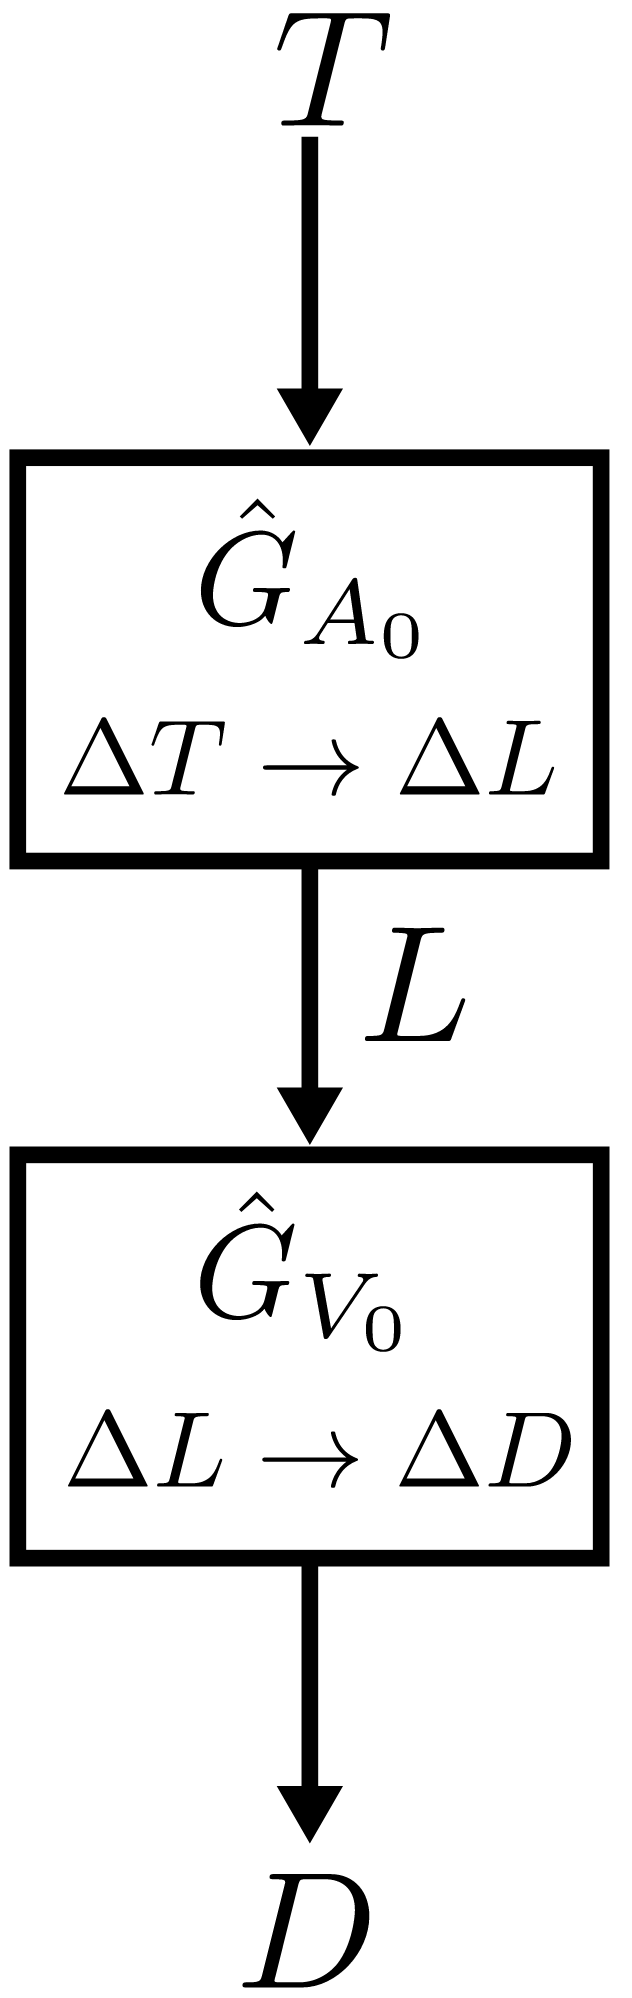
\includegraphics[height=.3\textheight]{TF_sub.png}
					\caption{Subsystem components of $\hat{G}_{RR}$. $\hat{G}_A$ (Actuator sub-transfer function) converts thermal fluctuations to axial displacement. $\hat{G}_V$ (Valve sub-transfer function) changes the effective orifice diameter when it is axially displaced by the Actuator.}
					\label{fig:TF_sub}
				\end{figure}
				\newcolumn

				{
					\setlength{\abovedisplayskip}{3pt}
					\setlength{\belowdisplayskip}{3pt}
					\setlength{\abovedisplayshortskip}{2pt}
					\setlength{\belowdisplayshortskip}{2pt}

					The complete transfer function in Figure~\ref{fig:TF_RR} converts the relationship
					\begin{equation}
						D = A_1 \Delta T + A_0
					\end{equation}
					
					to the system-representative form
					
					\begin{equation}
						D = \frac{dD}{dT} \Delta T + D_{ref}
					\end{equation}

					The reference value $D_{ref}$ represents the diameter size when $T_{amb} = T_{ref}$; its value must equal $A_0$, precisely determined by the machined dimension of certain critical parts.
					The control derivative term $\frac{dD}{dT}$ increases the diameter by $\Delta D$ as $T_{amb}$ changes; its value must equal $A_1$, determined by part dimensions and material properties.
					This derivative can be expanded as a series of sub-transfer functions (Figure~\ref{fig:TF_sub});
					the upper system represents the actuator subsystem's conversion of temperature to deflection,
					whereas the lower system represents the valve's translation to diameter changes as driven by the actuator.
					These will drive the core subsystem specifications.

					The required system transfer function can now be represented in its complete form:
					\RRfull

					\quad where

					\setlength{\jot}{2pt}

					\begin{align*}
						\frac{dL}{dT} &\text{ is determined by the actuator,} \\[6pt]
						\frac{dD}{dL} &\text{ is determined by the valve, and} \\[6pt]
						D_{ref} &\text{ is set the valve's initial position.}
					\end{align*}
				}

			\end{multicols}

			Though these values only specify the functional output of each subsystem, the selected design must exhibit a simple architecture with minimal degrees of freedom and strictly first-order behavior
			to produce a precise, linear system output. Nevertheless, certain errors cannot be avoided, so specifying calibration capabilities allows unpredictable errors to be corrected when
			the device is manufactured.

			Rolldown of the governing equation

			\begin{equation}
				\hat{G}_{RR} = \hat{G}_{A_0} \hat{G}_{V_0} = \frac{dL}{dT} \frac{dD}{dL} = A_1
			\end{equation}

			into its specified subcomponents allows for an unconstrained enumeration of values\footnote{
				Any combination of $\hat{G}_{A_0}$ and $\hat{G}_{V_0}$ whose product equals $A_1$ is acceptable.
			} so long as each architecture supports a linear, precise output.
			These were iteratively selected and partially informed by the architecture selected and described in Chapter~\ref{chap:design}.
			Thus, the following rolldown will seem arbitrary at first until the full design architecture is revealed. The selected valve architecture best supports a transfer function of

			\begin{equation}
				\hat{G}_{V_0} = - \sqrt{\frac{2}{\pi}} = \GV
			\end{equation}

			necessitating an actuator transfer function of

			\begin{equation}
				\hat{G}_{A_0} = \frac{A_1}{- \sqrt{\frac{2}{\pi}}} = - \sqrt{\frac{\pi}{2}} (\AoneExact) = \GA
			\end{equation}

			Finally, the valve must govern the reference value $D_{ref}$ such that 
			
			\begin{equation}
				D_{ref} = A_0 = \AzeroExact
			\end{equation}

			From these, we derive our first subsystem specifications:

			\newpage

			% \newpage
			\vspace{1em}
			\begin{mdframed}
				\begin{enumerate}
					\item Valve subsystem
						\begin{enumerate}
							\item \SpecVAA.
							\item \SpecVAB\\\SpecVABapp.
						\end{enumerate}
					\setcounter{enumi}{0}
					\item Actuator subsystem
						\begin{enumerate}
							\item \SpecAAA.
							\item \SpecAAB.
						\end{enumerate}
				\end{enumerate}
			\end{mdframed}

		\subsection{Mechanical Envelope rolldown}
		\label{subsec:intro:specs:ME}

			\setlength{\intextsep}{0pt}
			\begin{wrapfigure}{l}{2.6in}
				\centering
				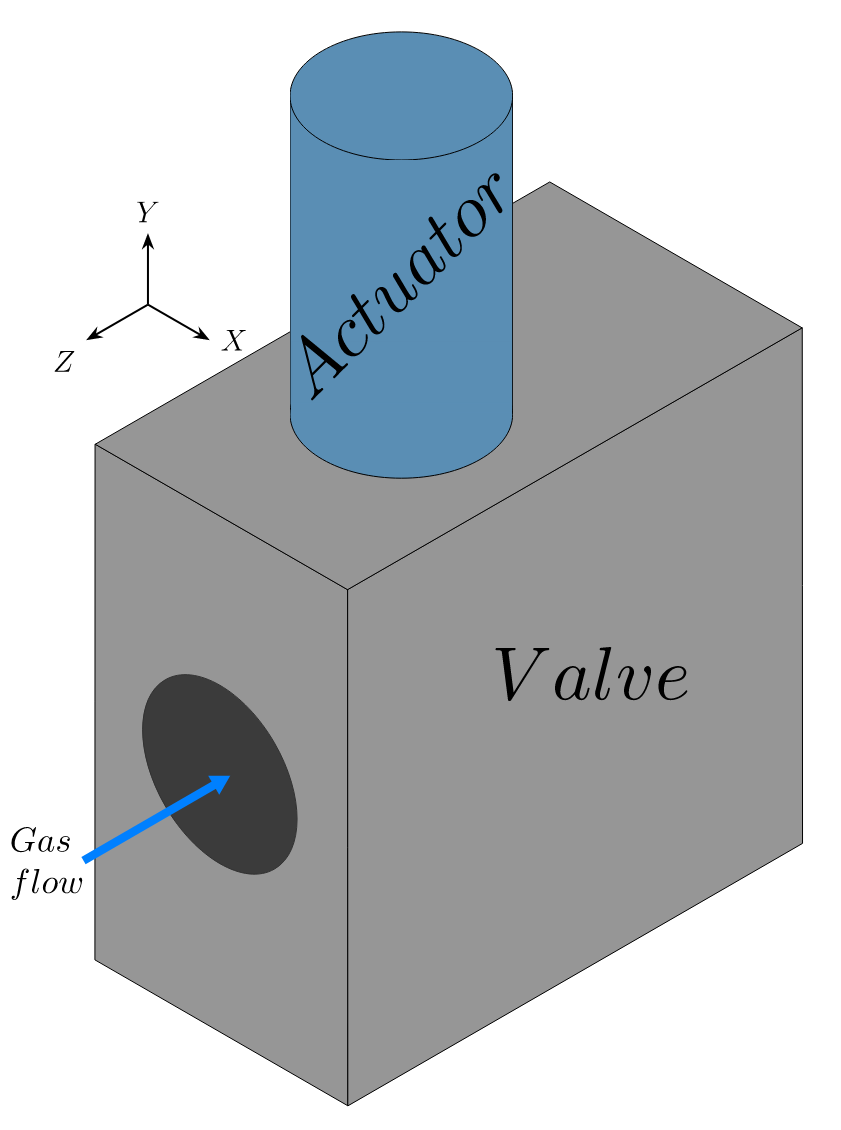
\includegraphics[height=3.5in]{Axes.png}
				\caption{Reference axes}
				\label{fig:axes}
			\end{wrapfigure}

			The Mechanical Envelope (\SI{10}{\centi\meter} in each direction) can be defined along three principal axes in a right-hand coordinate system,
			depicted in Figure~\ref{fig:axes}:

			% NOTE - These are consistent with the main CAD assembly axes
			\begin{itemize}
				\item The ``Longitudinal'' (Z) axis runs upstream along the direction of gas flow
				\item The ``Vertical'' (Y) axis points directly upwards
				\item The ``Lateral'' (X) axis points right as one looks downstream
			\end{itemize}


			If the assembly is stacked vertically as shown, each subsystem must share the space along the Y axis and can use the full \SI{10}{\centi\meter} along the other axes.
			As with the sub-transfer functions, the division of the vertical mechanical envelope is partially informed by the final design architecture.
			These specifications are given in lateral (X), vertical (Y), and longitudinal (Z) dimensions, respectively.
			\color{white}Easter egg text, included to avoid a wrapfigure error below. ``How good and pleasant it is when brothers live as one, in unity!''\color{black}

			\newpage
			% \vspace{1em}
			\begin{mdframed}
				\begin{enumerate}
					\setcounter{enumi}{1}
					\item Valve subsystem
						\begin{enumerate}
							\setcounter{enumi}{1}
							\item \SpecVB.
						\end{enumerate}
					\setcounter{enumi}{2}
					\item Actuator subsystem
						\begin{enumerate}
							\setcounter{enumi}{1}
							\item \SpecAB.
						\end{enumerate}
				\end{enumerate}
			\end{mdframed}

		\subsection{Operational Conditions rolldown}
		\label{subsec:Intro:specs:cond}

			Many design decisions were driven by the properties of the gas flow being controlled. The device must withstand the high gas pressure, be compatible with hydrogen, and minimize heat transfer from the hot internal gas.
			This rolls down to the following subsystem specifications.
			Note that ``wetted'' components are those in contact with the internal gas.

			\vspace{1em}
			\begin{mdframed}
				\begin{itemize}
					\setcounter{enumi}{2}
					\item Valve subsystem
						\begin{enumerate}
							\setcounter{enumi}{2}
							\item \SpecVCA.
							\item \SpecVCB.
							\item \SpecVCC.
						\end{enumerate}
					\setcounter{enumi}{2}
					\item Actuator subsystem
						\begin{enumerate}
							\setcounter{enumi}{2}
							\item \SpecACA.
						\end{enumerate}
				\end{itemize}
			\end{mdframed}
		
			\subsection{Final Subsystem Specifications}
		\label{subsec:intro:spec:final}

			The final system requirements and subsystem specifications are presented in Table~\ref{tab:specs} in the Appendix.

			The final design architecture was strictly screened to meet these specifications to ensure that the \device\ exhibits a passive, linear, precise output with simple, compact, high-strength components.

\chapter{Final Design of the \device}
\label{chap:design}

	\section{System Architecture Overview}
	\label{sec:design:overview}

		The \device\ contains and seals high-pressure hydrogen gas and delivers precise thermomechanical actuation with proven, aerospace-grade technology.
		It also introduces a novel variable-diamond orifice that overcomes several weaknesses of existing valve architectures.
		The device comprises a valve assembly, with a threaded housing, orifice components, and associated hermetic seals; and an actuator assembly, with a bimetallic architecture and calibration system.
		The full assembly is pictured in Figures \ref{fig:mainIsometric} and \ref{fig:mainExploded}.

		\begin{figure}[H]
			\begin{minipage}{.49\textwidth}
				\centering
				% 
\includegraphics[width=.85\textwidth]{CompleteAssemblyExploded.png}
				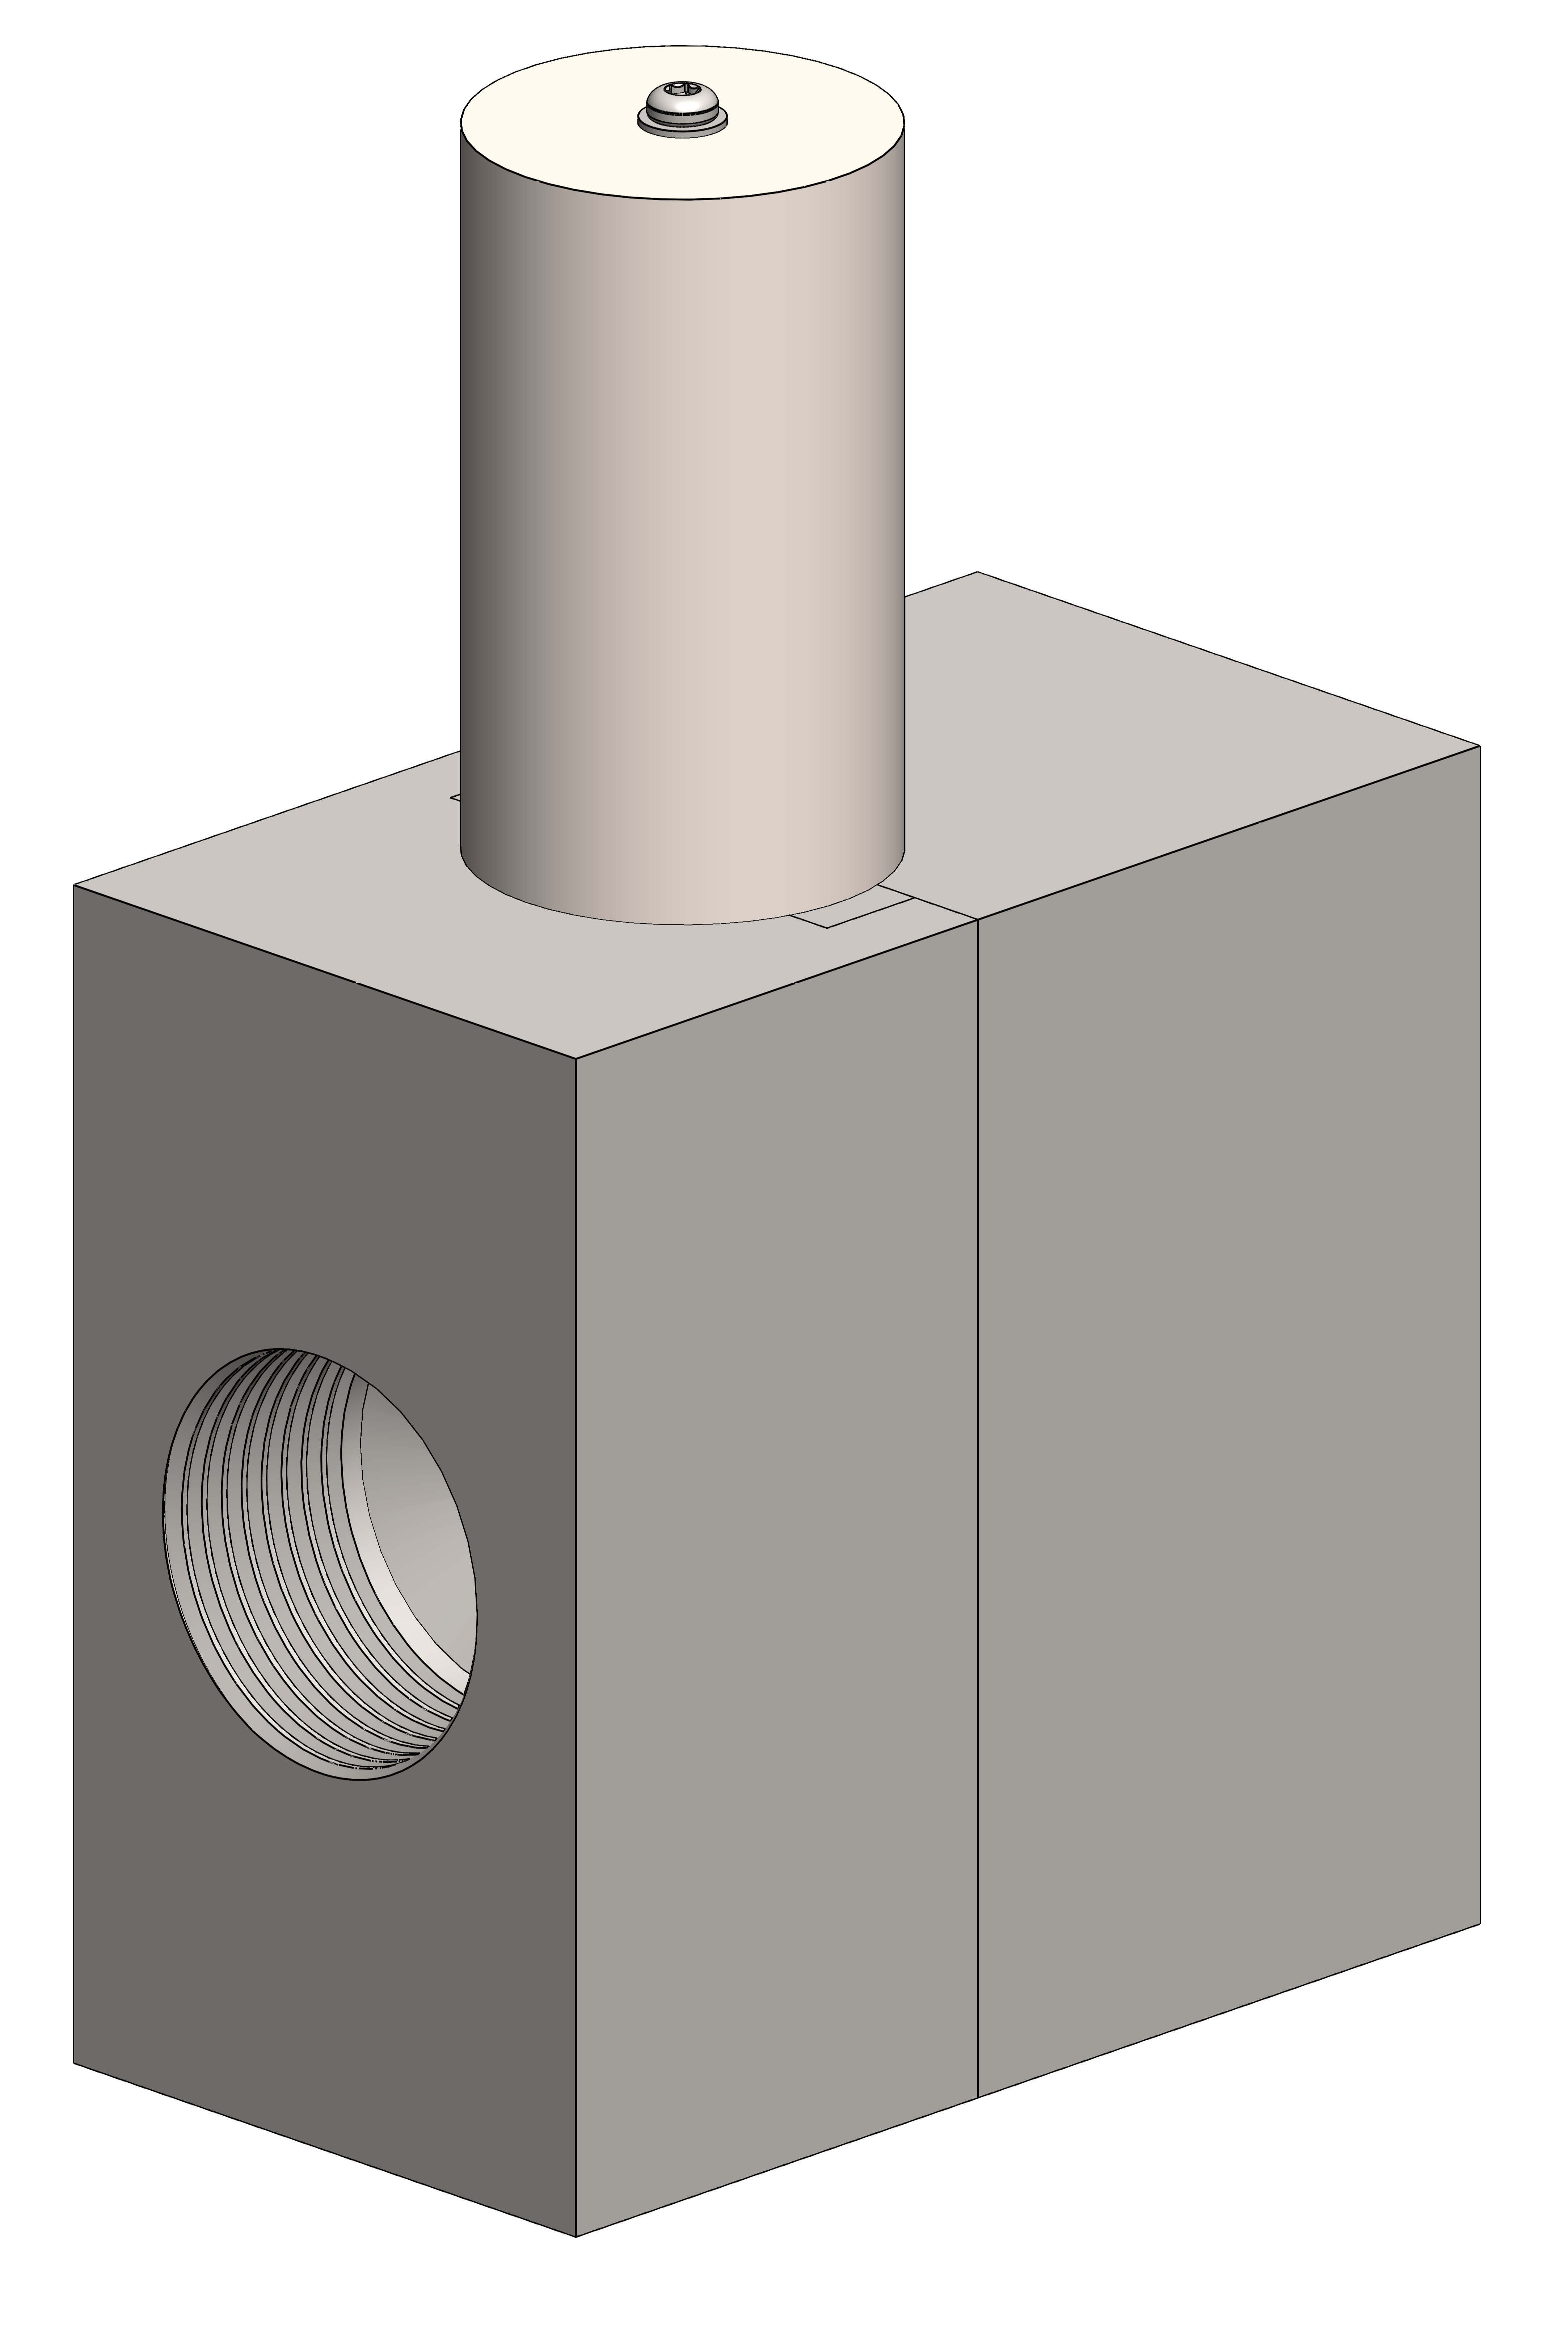
\includegraphics[width=.75\textwidth]{PTCD.png}
				\caption{Complete assembly exploded view}
				\label{fig:mainIsometric}
			\end{minipage}
			\hfill
			\begin{minipage}{.49\textwidth}
				\centering
				\includegraphics[width=.75\textwidth]{exp_qual.png}
				\caption{Sub-assembly identification}
				\label{fig:mainExploded}
			\end{minipage}
		\end{figure}

	The valve orifice at the heart of the PTCD comprises two plates with identical square holes cut at 45$^\circ$ angles.
		One plate is fixed to the valve housing; the other is free to move vertically driven by the valve stem.\footnote{This report will refer to the hole in the mobile Valve Orifice part and the hole in the fixed Housing as the leading and trailing orifice, respectively.}
		The two square holes lie flush and are vertically offset such that only a small square opening appears between the valve inlet and its outlet. 

		\begin{wrapfigure}{l}{.2\textwidth}
			\centering
			
\includegraphics[height=1.5in]{orifice.png}
			\caption{Orifice geometry}
			\label{fig:orifice}
		\end{wrapfigure}

	
		If the two holes were circles, they would resemble a Venn diagram; thus, as pictured in Figure~\ref{fig:orifice}, the diamond-shaped overlap between these squares constitutes the valve orifice. 
		The lower (blue) square is cut into the central moving plate such that as the valve stem drives the plate downwards, the orifice (the gray overlap region) constricts.
		
		A bimetallic actuator is fixed above the housing and welded to the valve stem; it drives the central orifice as it responds to temperature changes.
		The outer material, ALLVAR, shrinks when heated, while the inner material, aluminum, expands.
		Thus, as pictured in Figure~\ref{fig:active_diagram}, as the ambient temperature increases, the actuator drives the valve stem downwards, shrinking the orifice. 
		As the temperature decreases, the actuator pulls the stem back up, opening the orifice again. Across the total design temperature range, the actuator expands \SI{267}{\micro\meter}, driving the valve an equal distance.

		\begin{figure}[H]
			\centering
			\begin{minipage}{.45\textwidth}
				\centering
				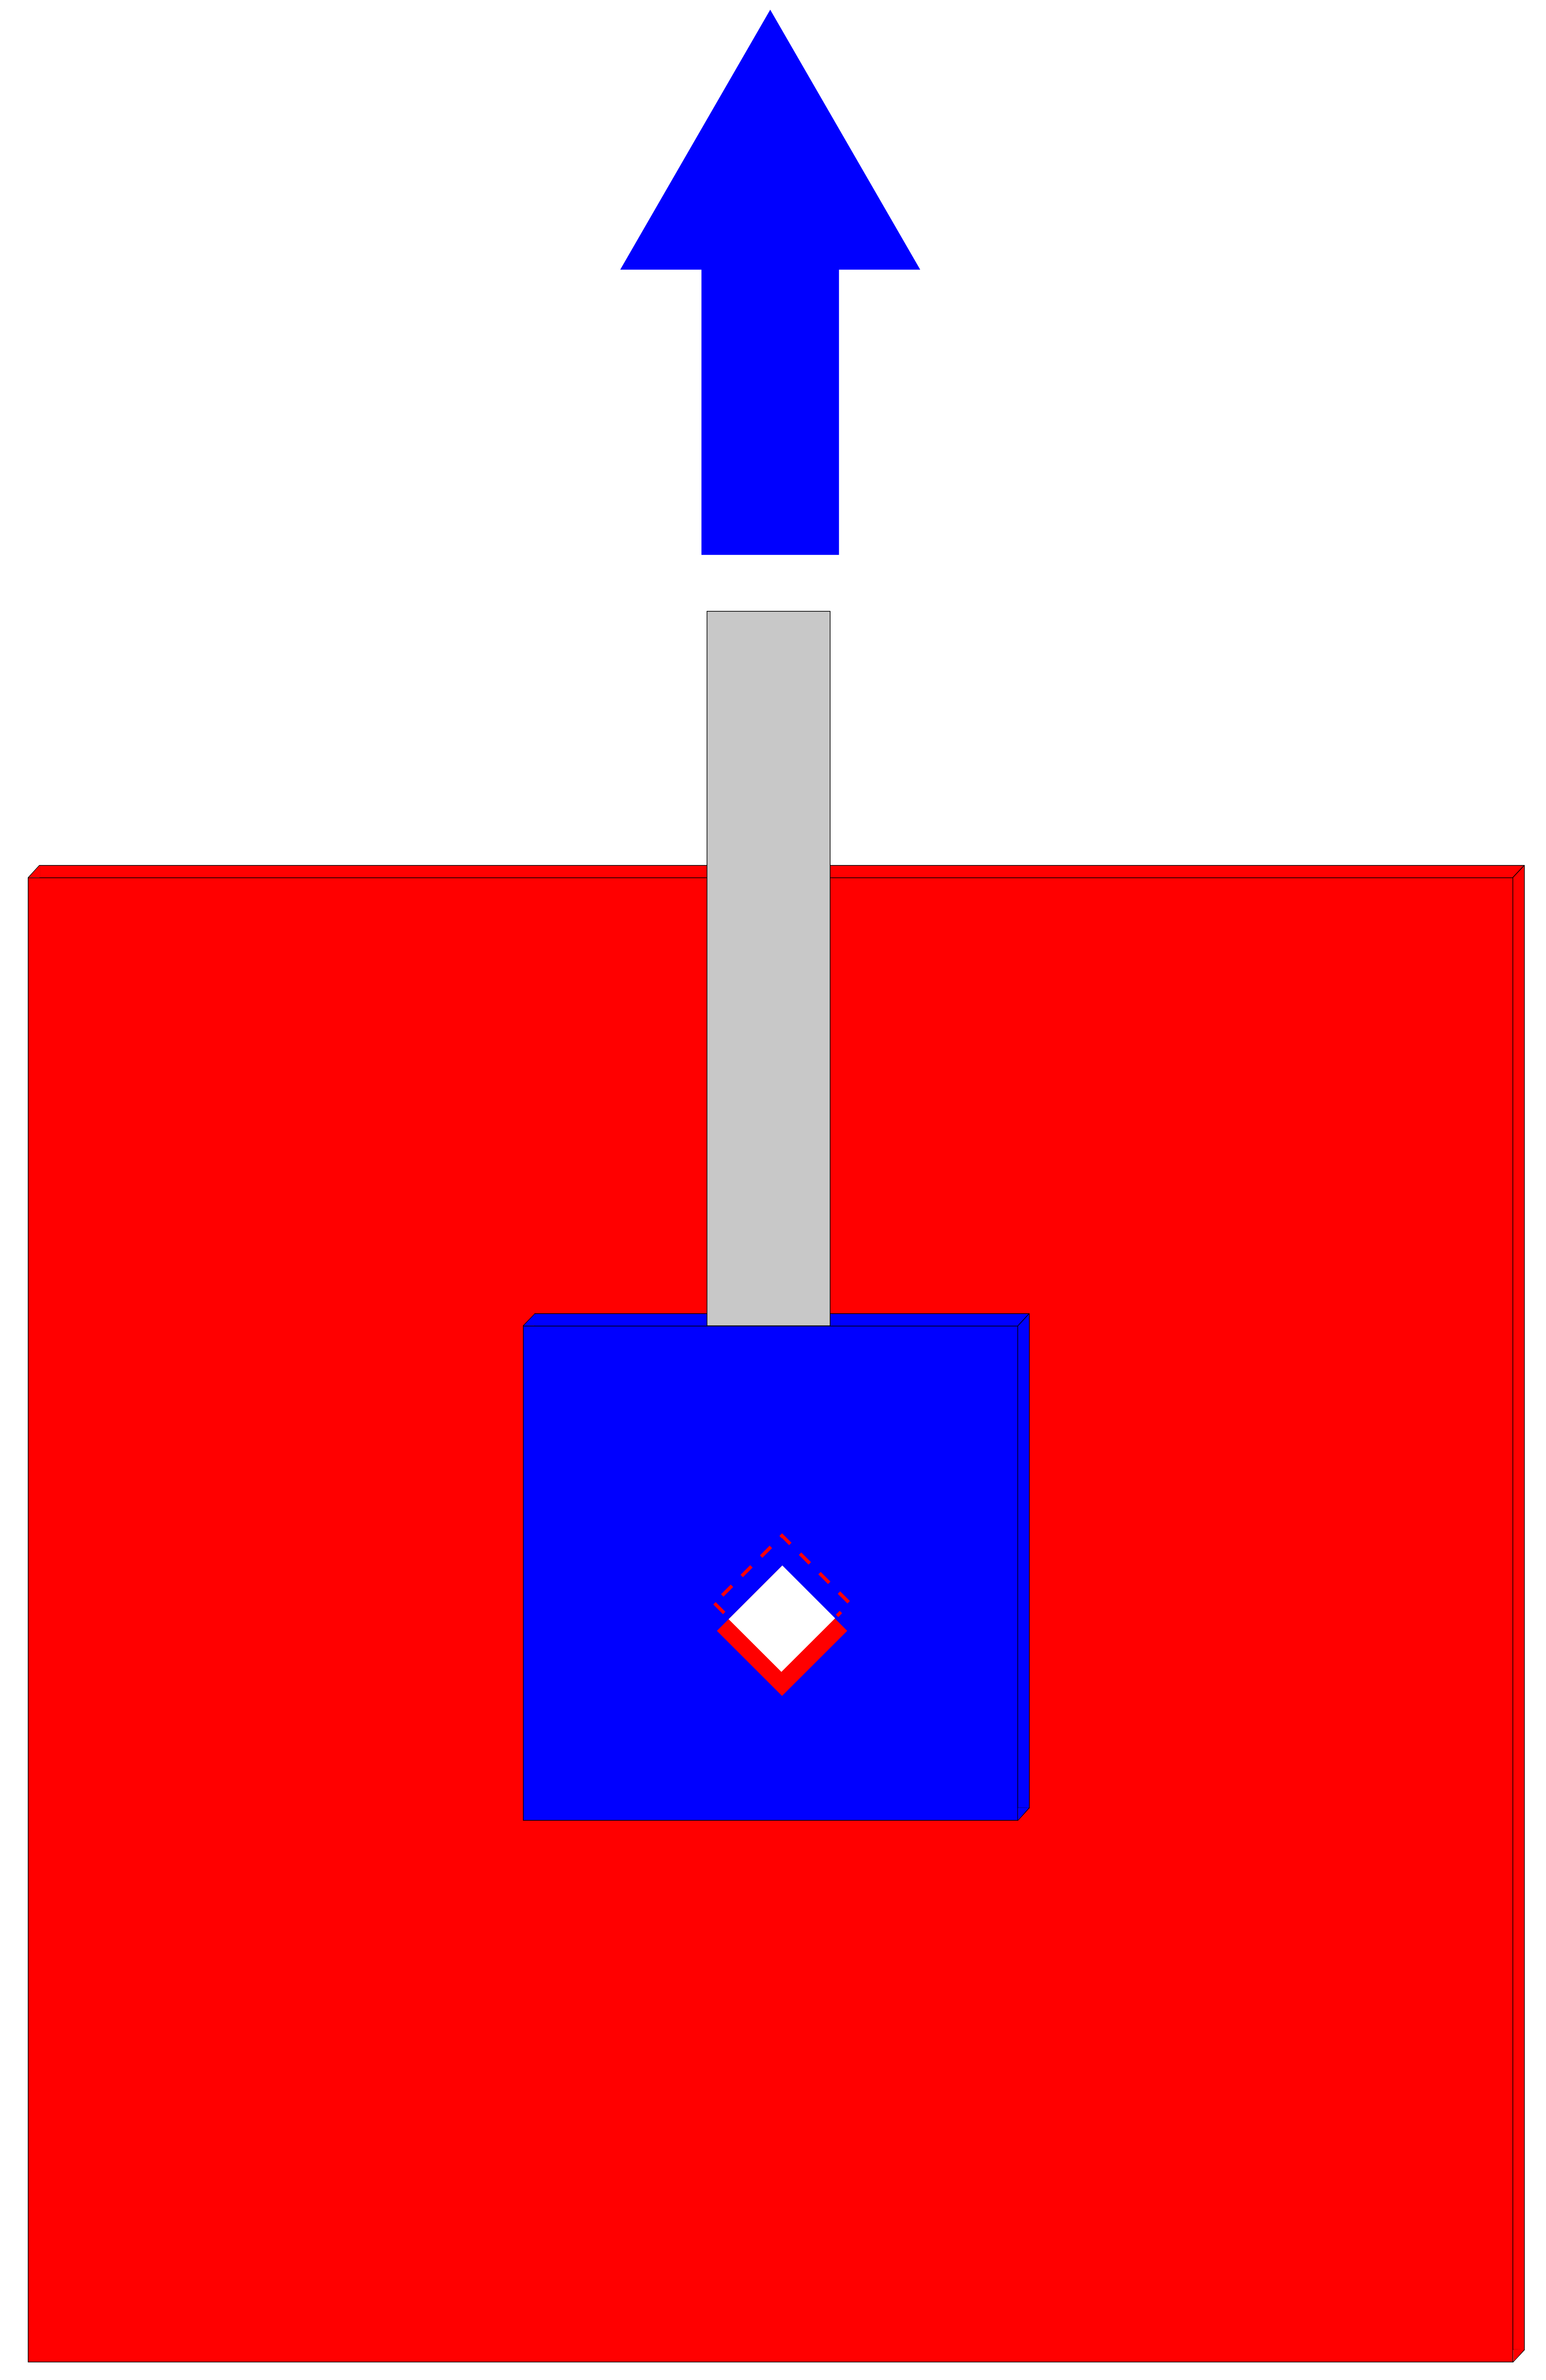
\includegraphics[width=.5\textwidth]{active_cold.png}
				\subcaption{Cooling actuation}
				\label{fig:active_cold}
			\end{minipage}
			\hfill
			\begin{minipage}{.45\textwidth}
				\centering
				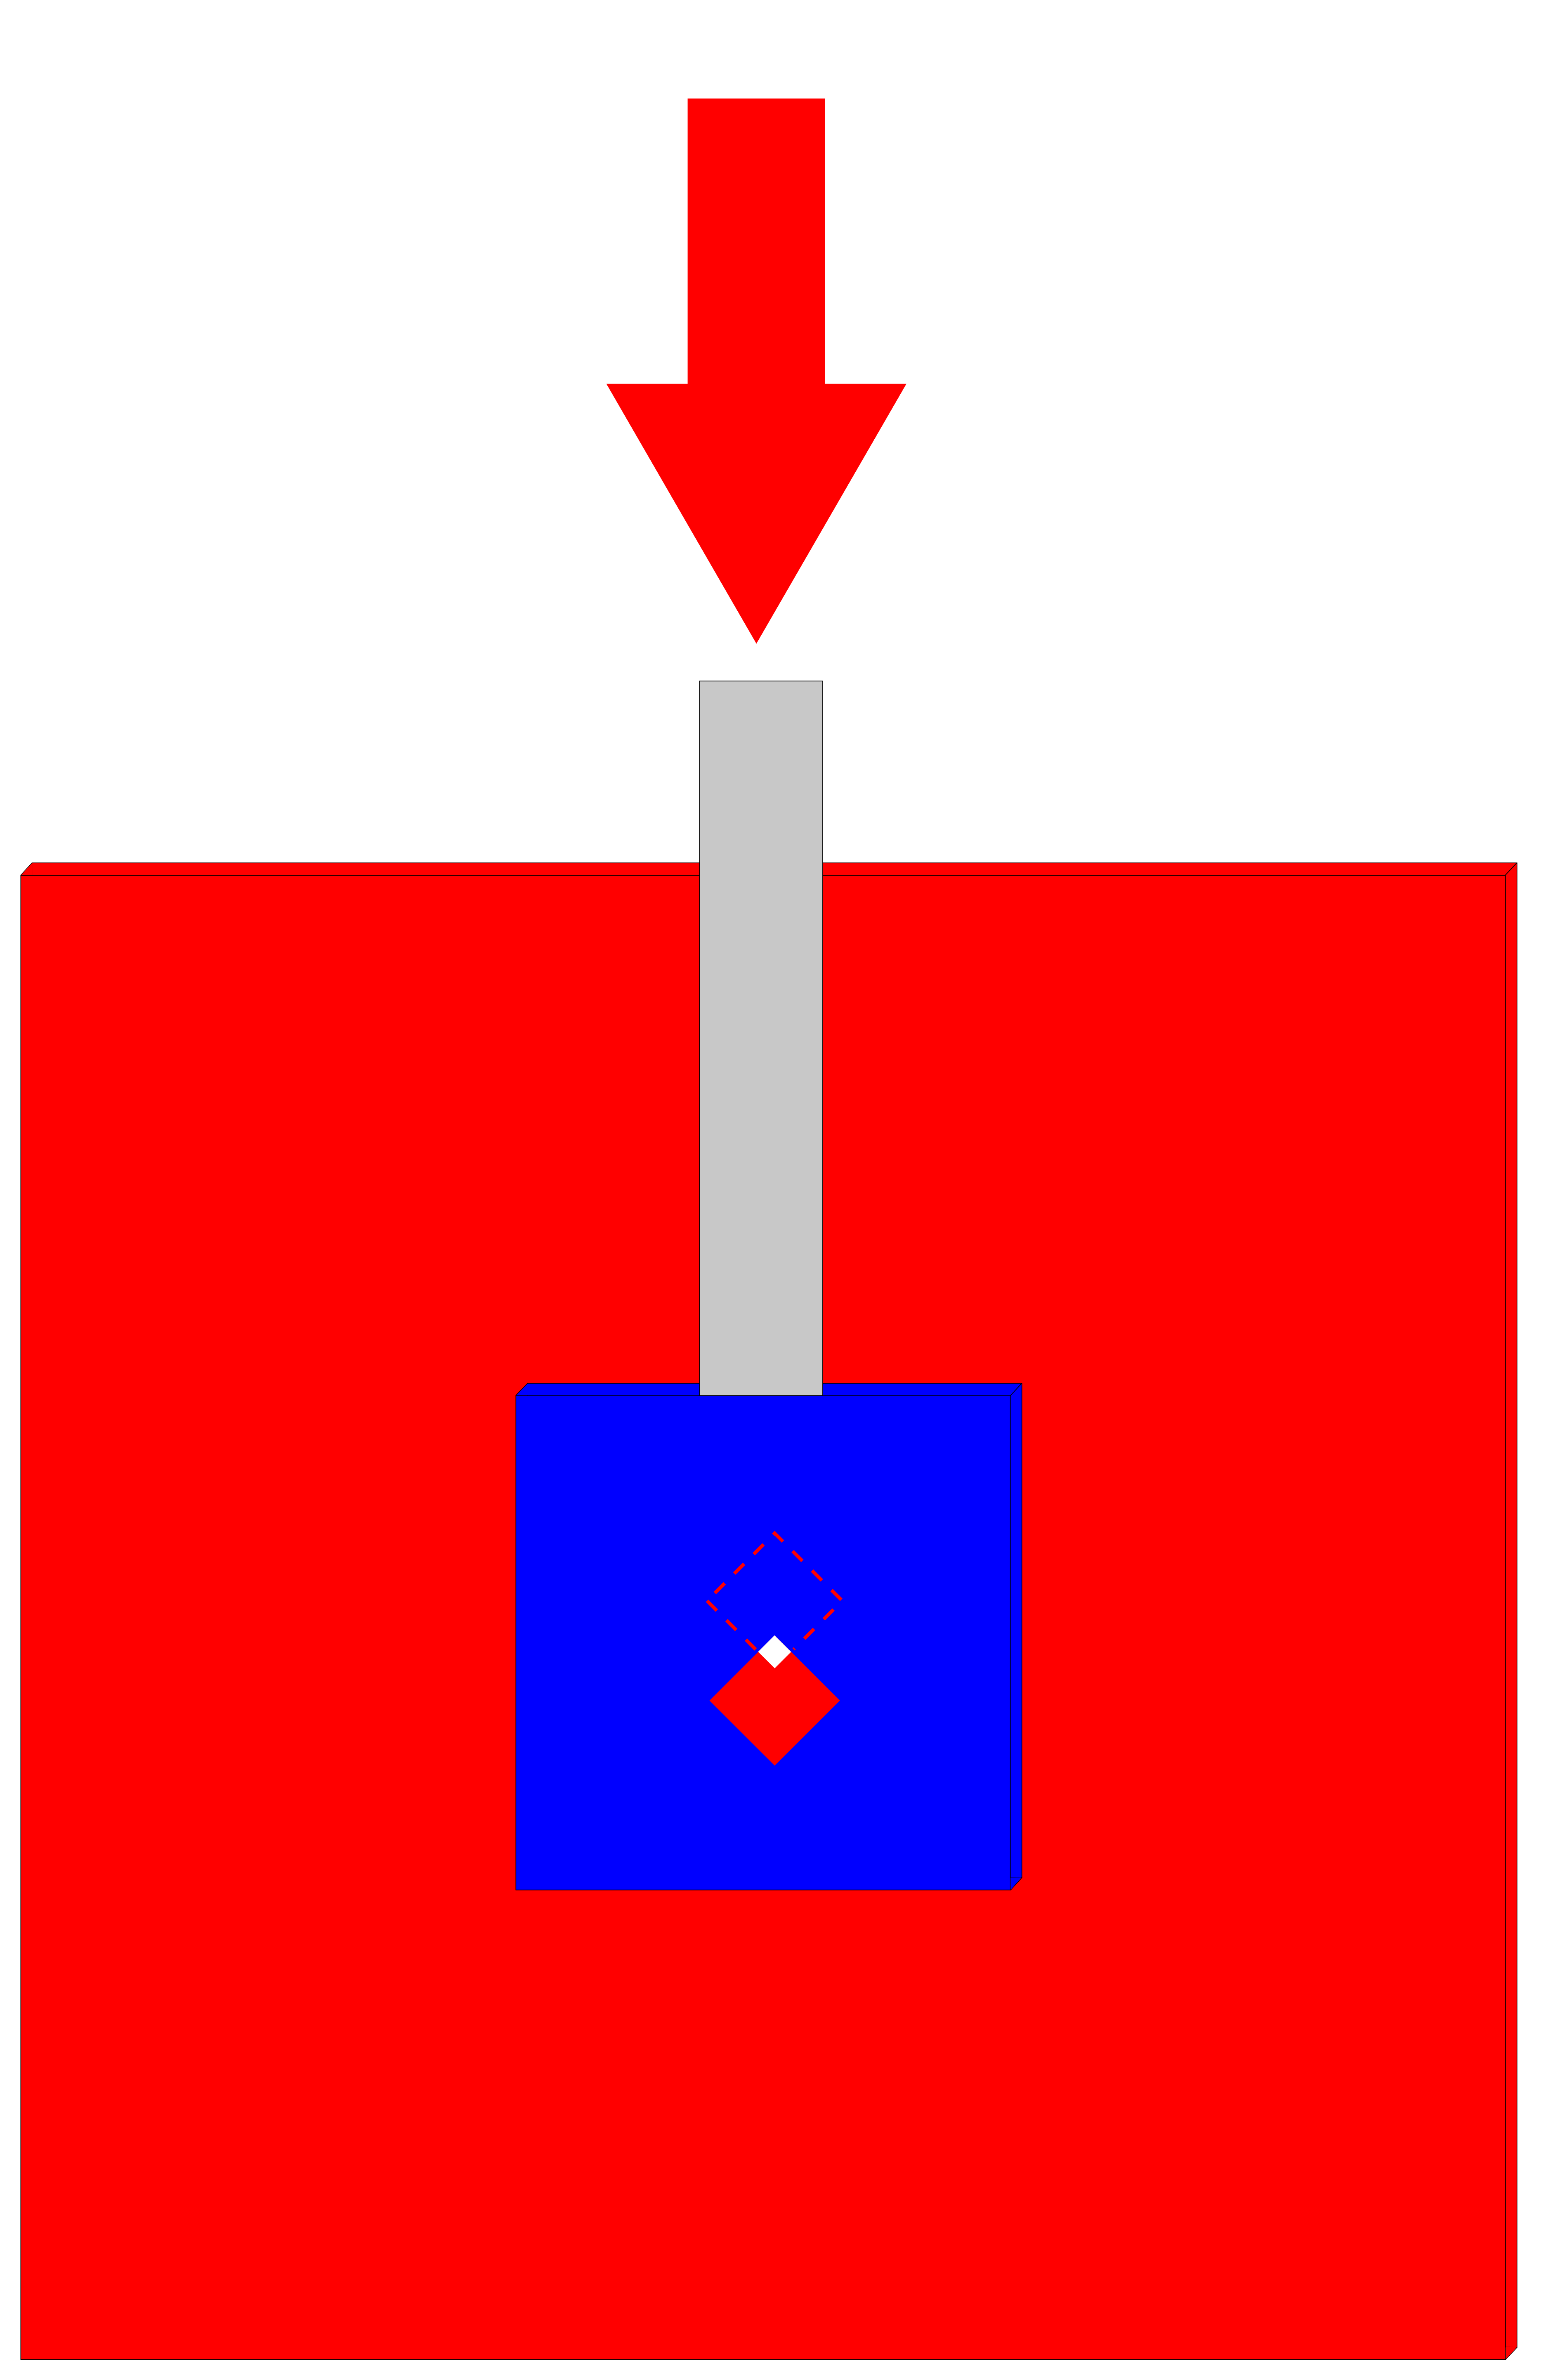
\includegraphics[width=.5\textwidth]{active_hot.png}
				\subcaption{Heating actuation}
				\label{fig:active_hot}
			\end{minipage}
			\caption{Mechanism of the \device}
			\label{fig:active_diagram}
		\end{figure}

		\subsection{Valve Subsystem}
		\label{subsec:design:overview:valve}

			\begin{wrapfigure}{l}{.2\textheight} % .32\textheight is the width, but the image is roughly square
				\centering
				% 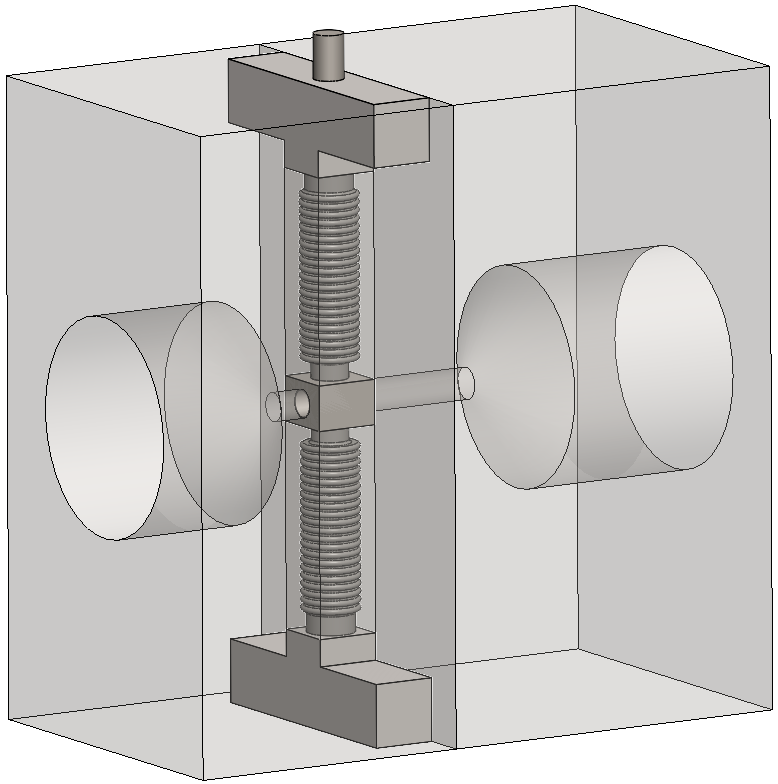
\includegraphics[height=.4\textheight]{Valve_full.png}
				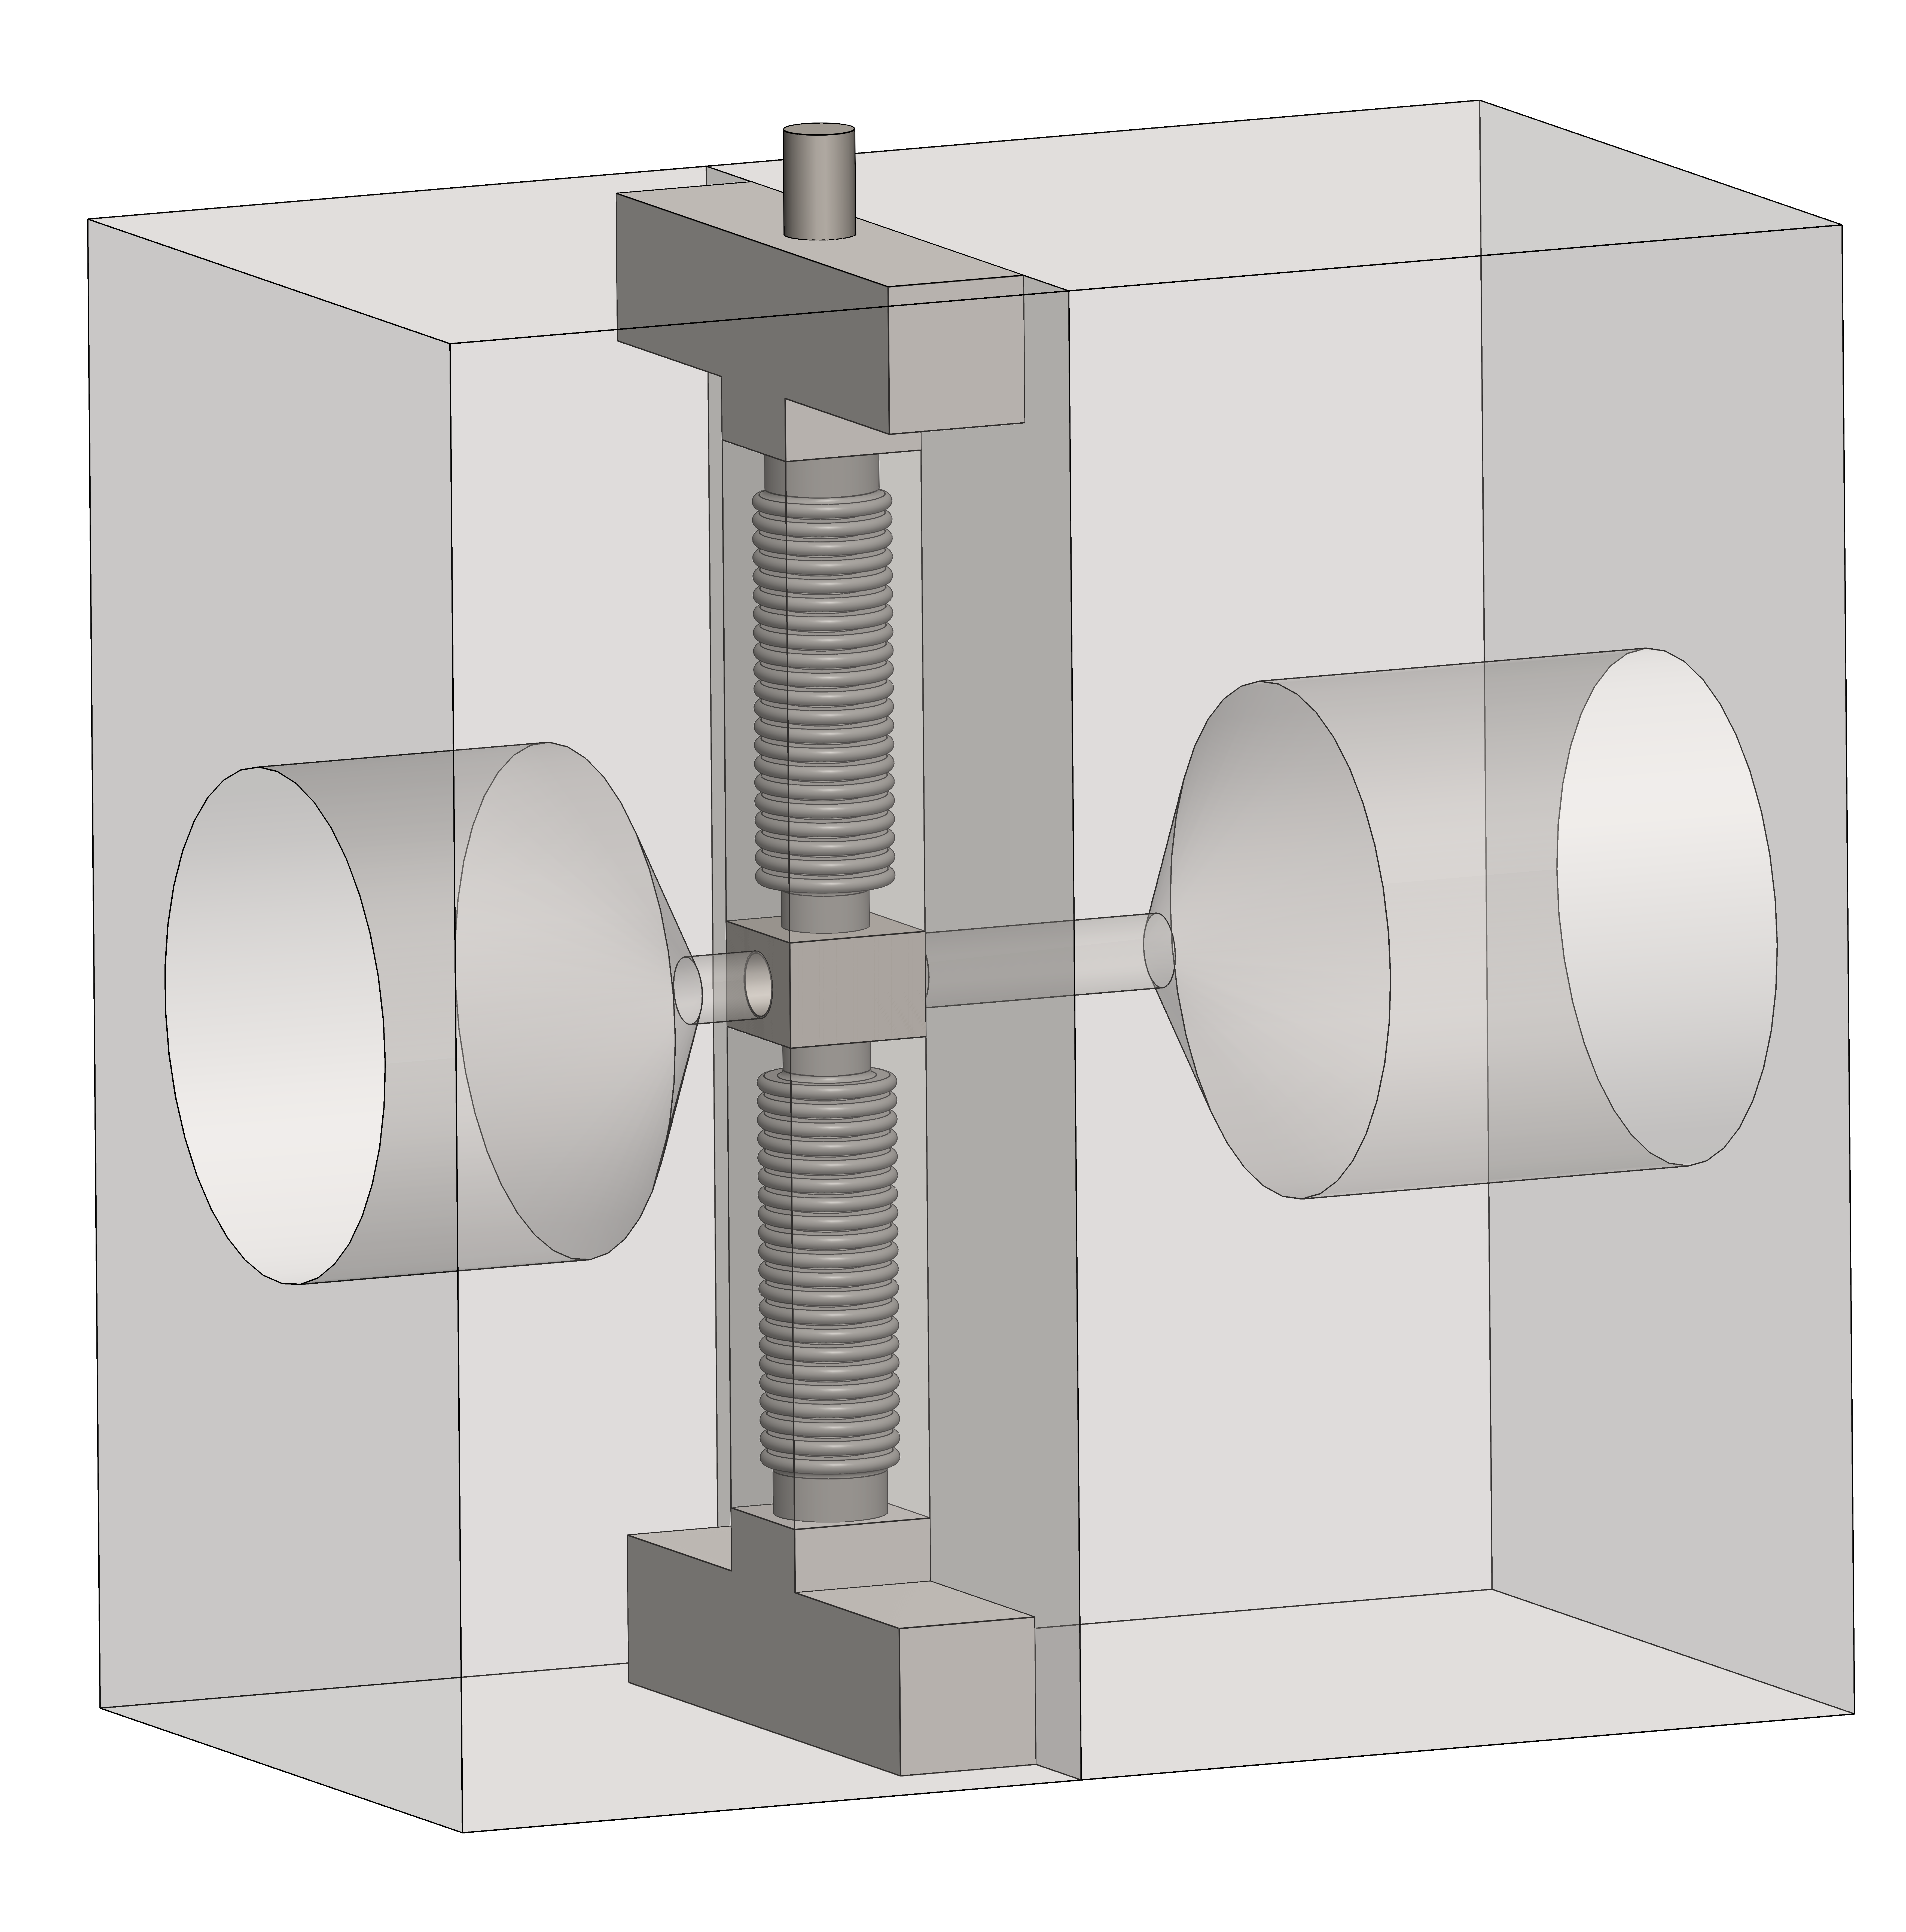
\includegraphics[height=.2\textheight]{Valve_full_qual.png}
				\caption{Valve subsystem}
				\label{fig:valve_full}
			\end{wrapfigure}

			The valve subsystem (Figures \ref{fig:valve_full}, \ref{fig:valve_exploded}, \ref{fig:valve_ID}) contains the high-pressure gas and restricts its flow, only allowing gas to exit through its small internal orifice.
			Its housing is coupled to stainless steel pipes by a test engineer and provides the structural support necessary to hold the internal pressure.
			The leading-orifice component nests between four walls and slides vertically within the assembly.
			Attached is the valve stem, welded to and driven by the actuator.
			This housing penetration is hermetically sealed by a bellows. A corresponding valve stem-bellows pair extends through the bottom of the housing to balance the resultant pressure forces.

			\begin{figure}[H]
				\begin{minipage}{.49\textwidth}
					\centering
					% 
\includegraphics[width=\textwidth]{Valve_exploded.png}
					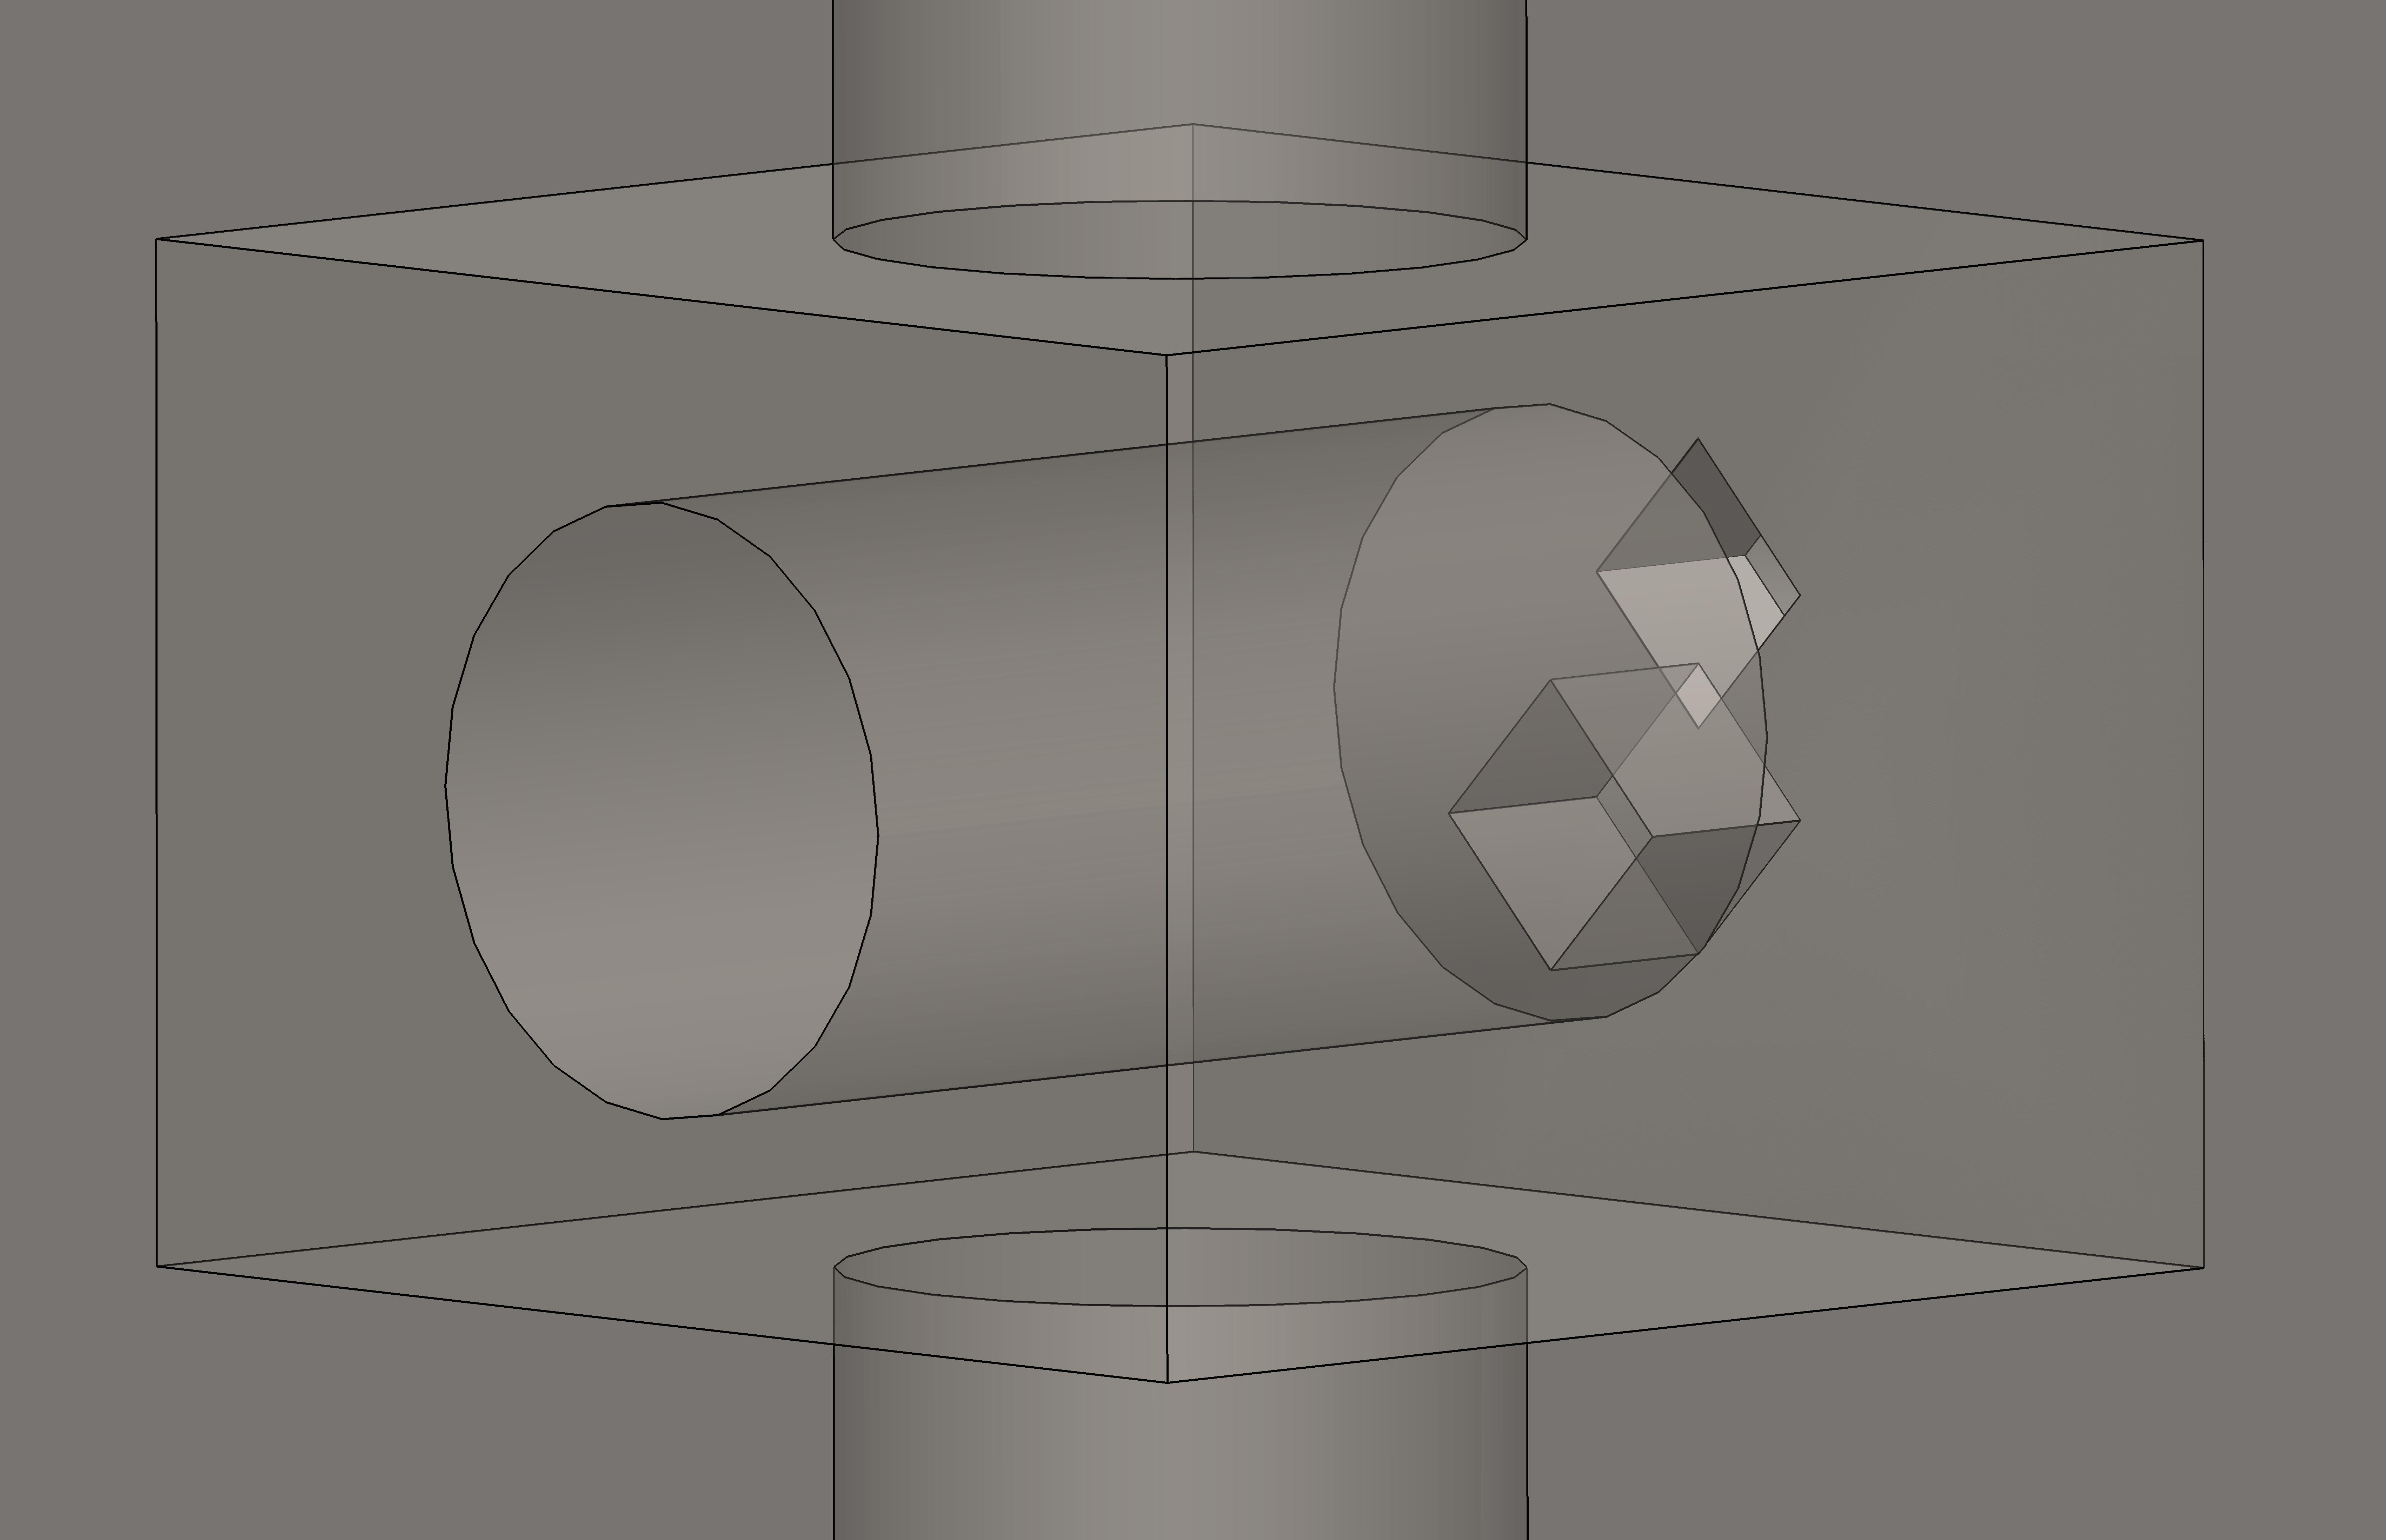
\includegraphics[width=\textwidth]{orif_assem_right_qual.png}
					\caption{Valve subsystem exploded view}
					\label{fig:valve_exploded}
				\end{minipage}
				\hfill
				\begin{minipage}{.49\textwidth}
					\centering
					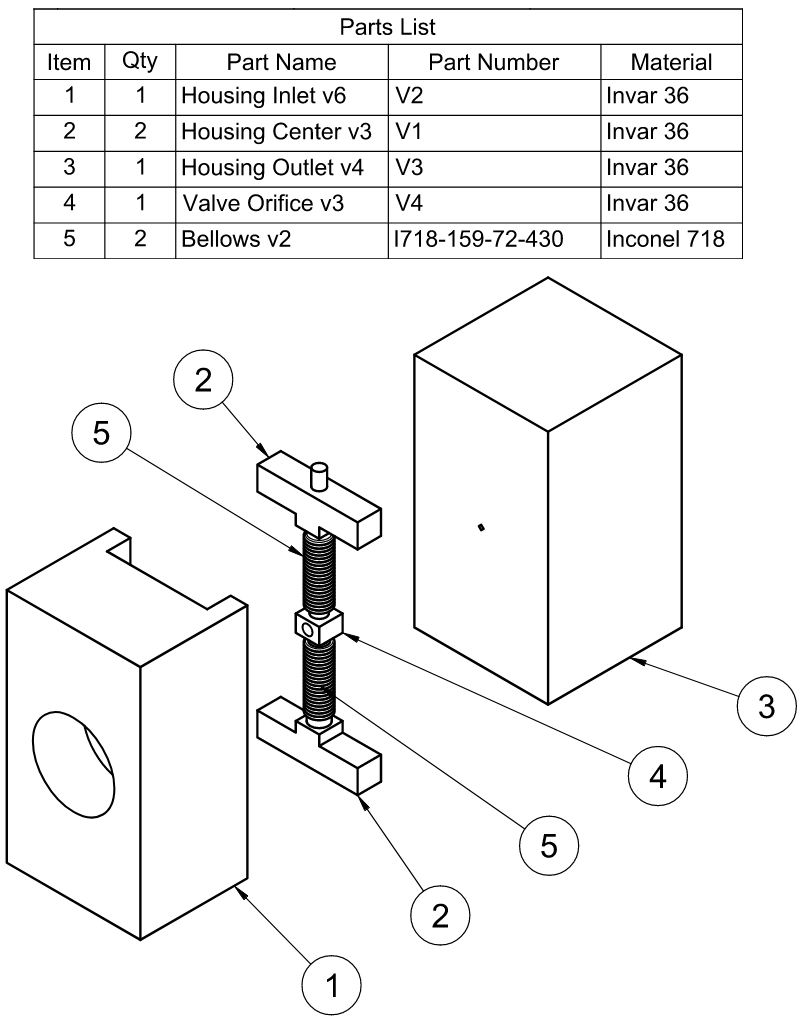
\includegraphics[width=\textwidth]{Valve_ID.png}
					\caption{Valve subsystem part identification}
					\label{fig:valve_ID}
				\end{minipage}
			\end{figure}

			The Valve Orifice (4) comprises the leading orifice hole near its center.
			The actuator drives its motion via the upper valve stem so that it moves freely up and down while the other parts remain fixed.
			It lies flush against the Housing Outlet (3), which comprises the trailing orifice hole and directs low-pressure gas out of the assembly through a pipe threaded into its rear.
			Together, these comprise the \device's orifice, shown in Figure~\ref{fig:orif_assem}.

			Lateral and longitudinal movement of the Valve Orifice are constrained by the Housing Inlet (1), which presses it against the face of the Outlet and restricts all motion to the vertical degree of freedom.
			The inlet and outlet butt together, leaving enough space in its central channel for the Valve Orifice to fit snugly between four walls.

			Two Housing Center pieces (2) plug the remaining gaps.
			They contain holes for the valve stems to slide through, guiding their motion.
			To hermetically seal these holes, a bellows (5) is welded between the Valve Orifice and each Housing Center.
			As the centerpiece moves up and down, the flexible bellows extend and contract, allowing for flexible, sealed penetration of the housing.
			The housing center and bellows are inserted as in Figure~\ref{fig:V1_bellows}.

			\newpage

			\begin{figure}[H]
				\begin{minipage}{4.5in}
			Figure~\ref{fig:cut_zooms} shows the orifice in full assembly.
			The leading orifice on the moving piece is positioned below the trailing orifice as prescribed in Figure~\ref{fig:orifice}.

					\medskip
					All components of the valve assembly are joined by Electron-Beam Weld (EBW), a precise method to attach flush faces against one another and nearly perfectly fuse them together.

					\medskip
					All machined parts are made of Invar 36\cite{ref_Invar_1897, ref_Invar_1920}, a Ni-Fe alloy renowned for its exceptionally low thermal expansion,
					ensuring high thermal stability under the expected temperature fluctuations.
				\end{minipage}
			\hfill
				\begin{minipage}{1.9in}
				\centering
				% 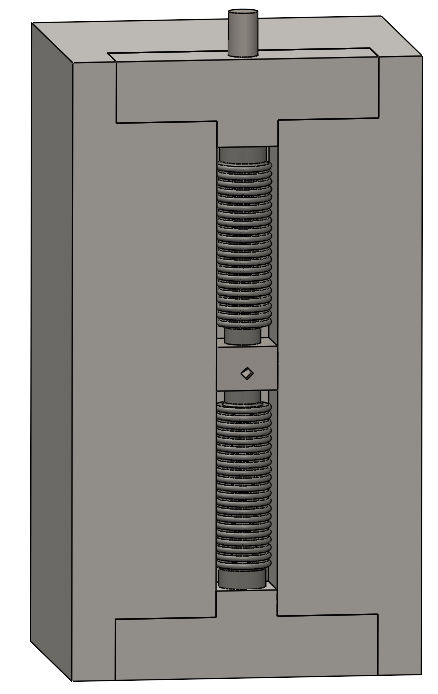
\includegraphics[height=4in]{V1_bellows.png}
				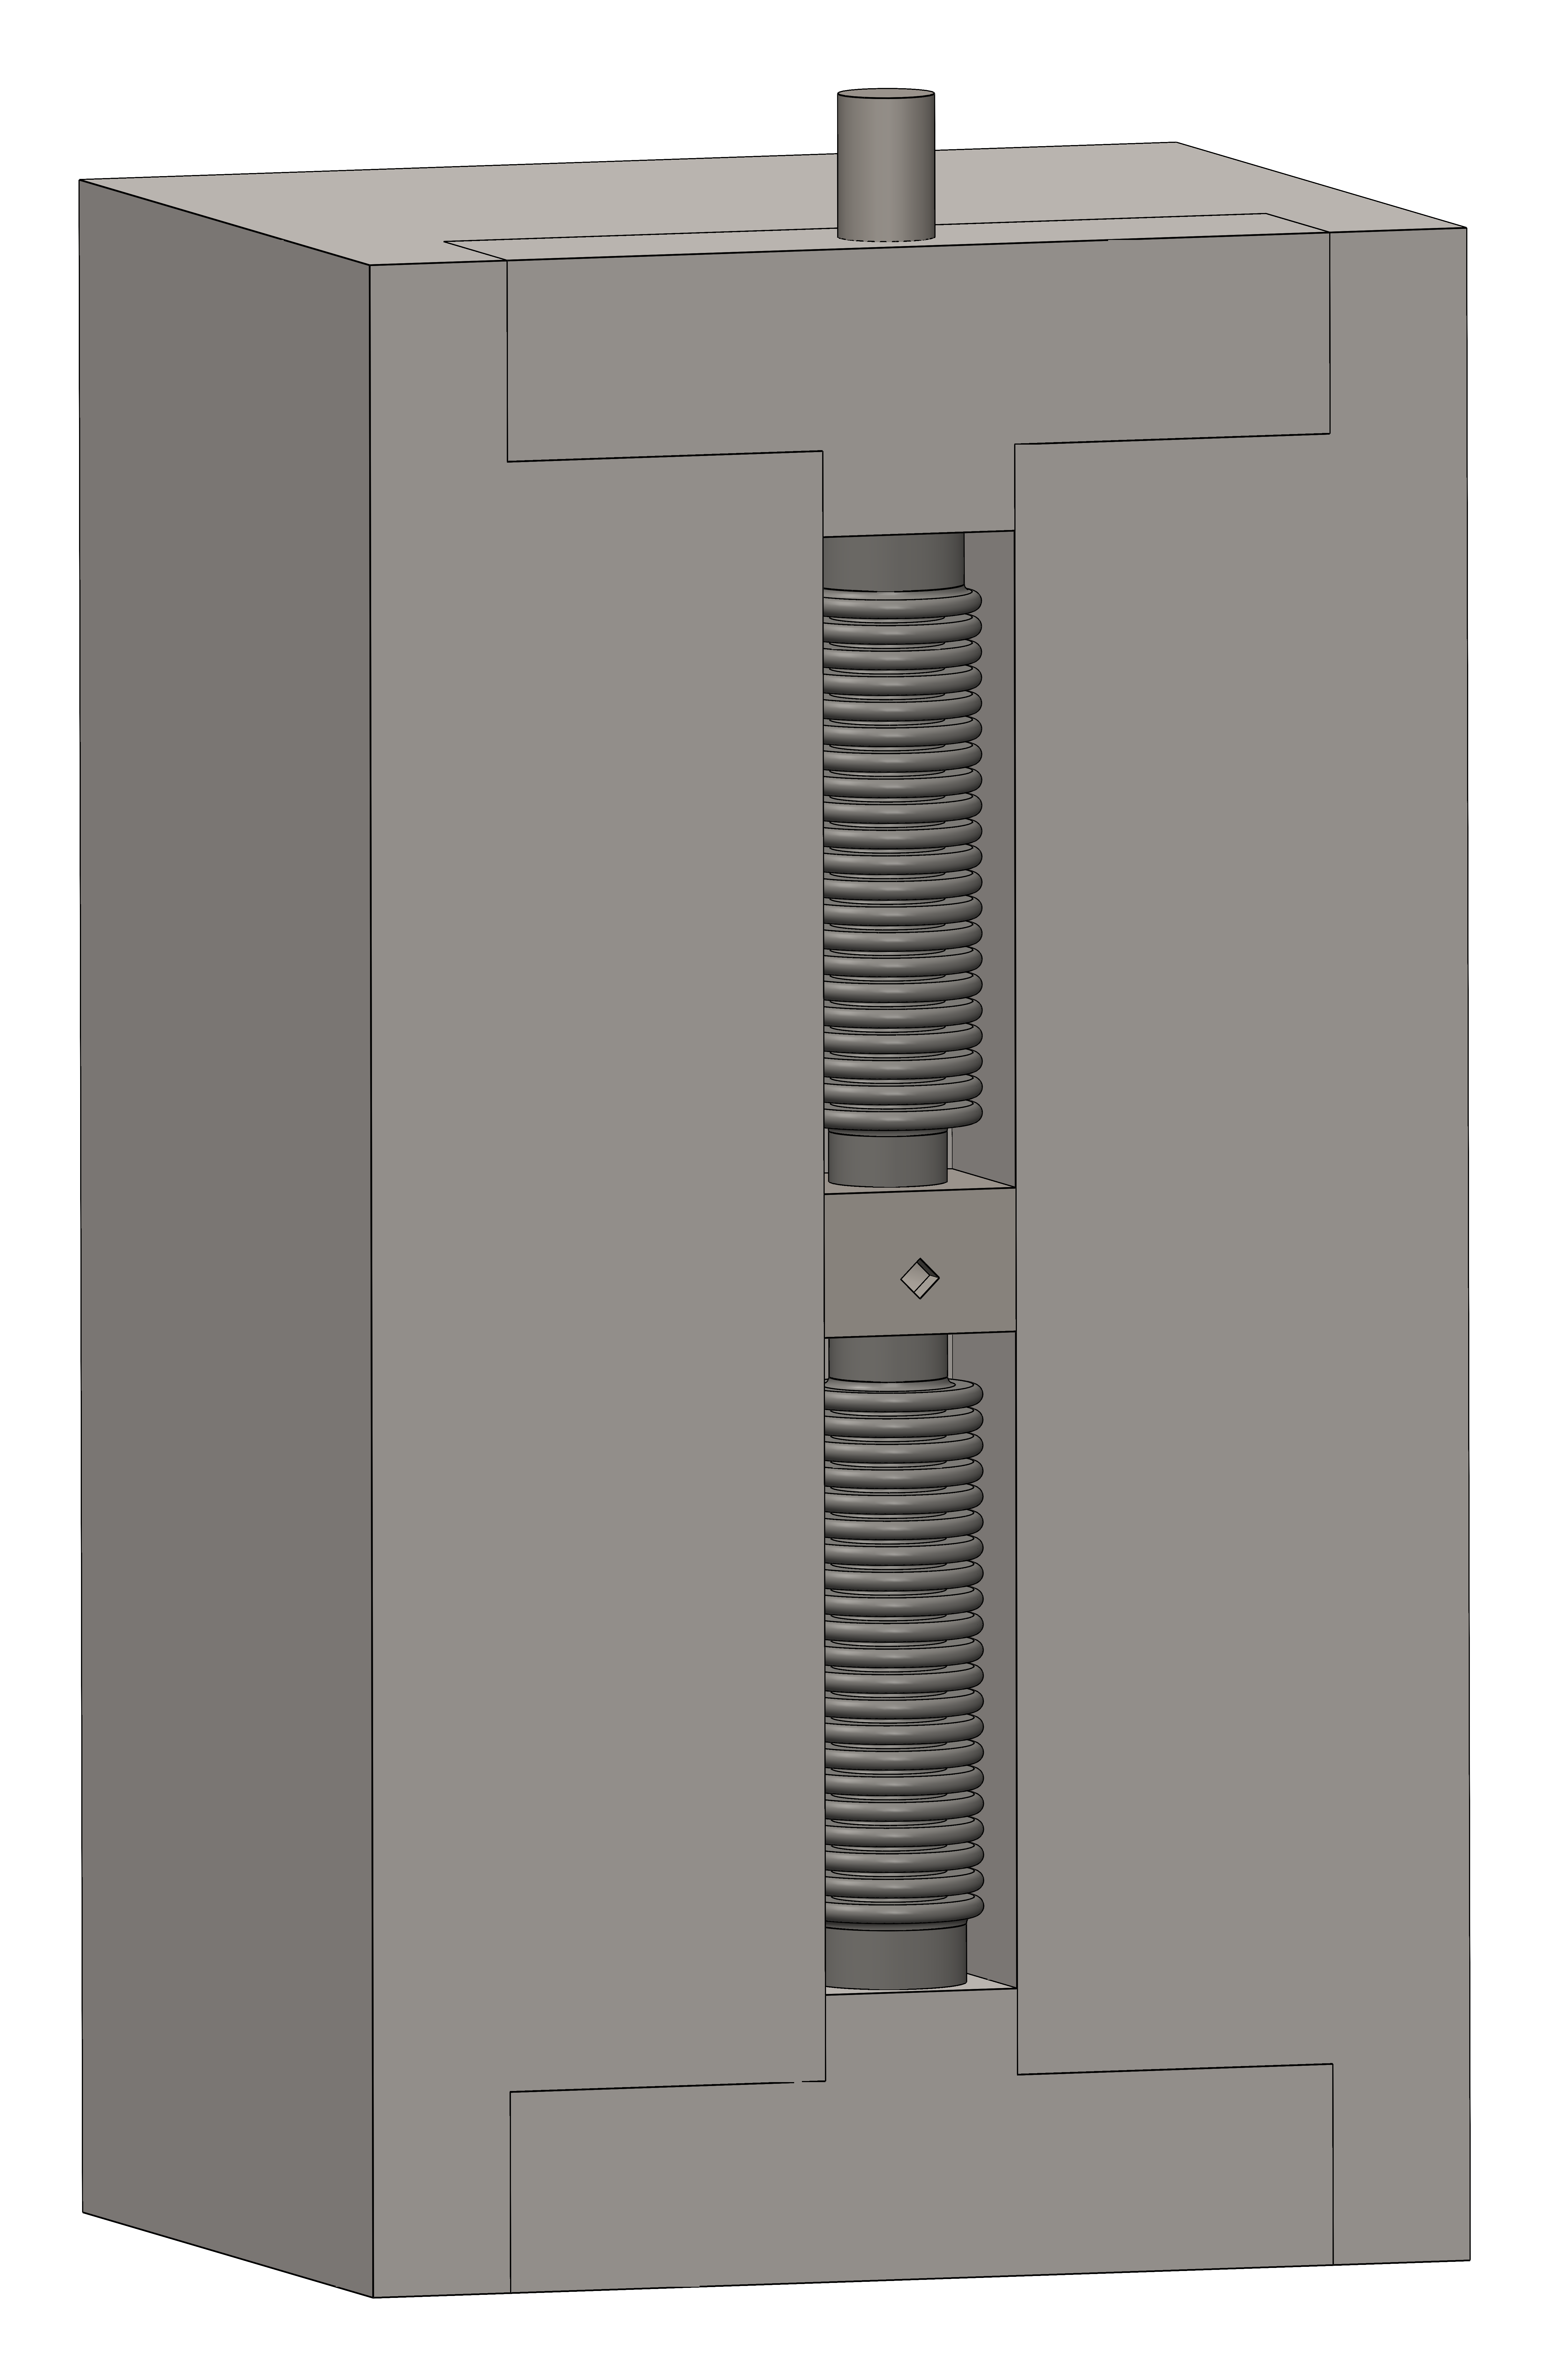
\includegraphics[height=3in]{V1_bellows_qual.png}
				\caption{Housing Center and bellows}
				\label{fig:V1_bellows}
				\end{minipage}
			\end{figure}

			\vspace{-1em}
			\begin{figure}[H]
					\centering
					\begin{subfigure}{0.45\textwidth}
							\centering
							% 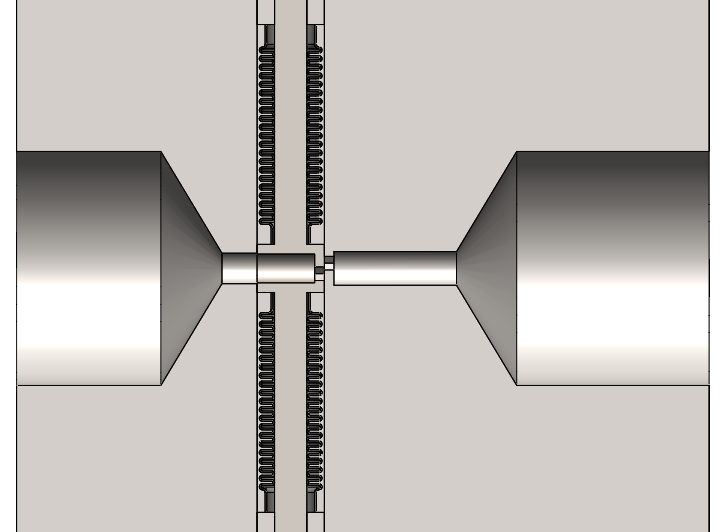
\includegraphics[width=\textwidth]{cut_zoom.png}
							\includegraphics[width=\textwidth]{cut_zoom_qual.png}
							\caption{Valve Subsystem, Section View}
							\label{fig:cut_zoom}
					\end{subfigure}
					\hfill
					\begin{subfigure}{0.39\textwidth}
							\centering
							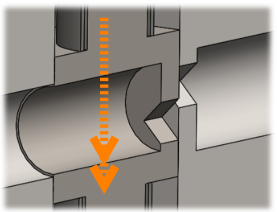
\includegraphics[width=\textwidth]{cut_zoom_zoom_crop.png}
							\caption{Valve, Section View (detail)}
							\label{fig:cut_zoom_zoom_crop}
					\end{subfigure}
					\caption{Section views}
					\label{fig:cut_zooms}
			\end{figure}

		\subsection{Actuator Subsystem}
		\label{subsec:design:overview:act}

			The actuator subsystem (Figures \ref{fig:act_full}, \ref{fig:act_exploded}, \ref{fig:act_ID}) sits atop the valve housing, where it maintains equilibrium with the surrounding ambient air temperature.
			It comprises an internal expansion rod to drive the valve stem, an external mount to suspend it from above, a screw and washer to secure them together, and a belleville washer to enable precise calibration.

			\begin{figure}[H]
				\centering
				\begin{minipage}{.4\textwidth}
					\centering
					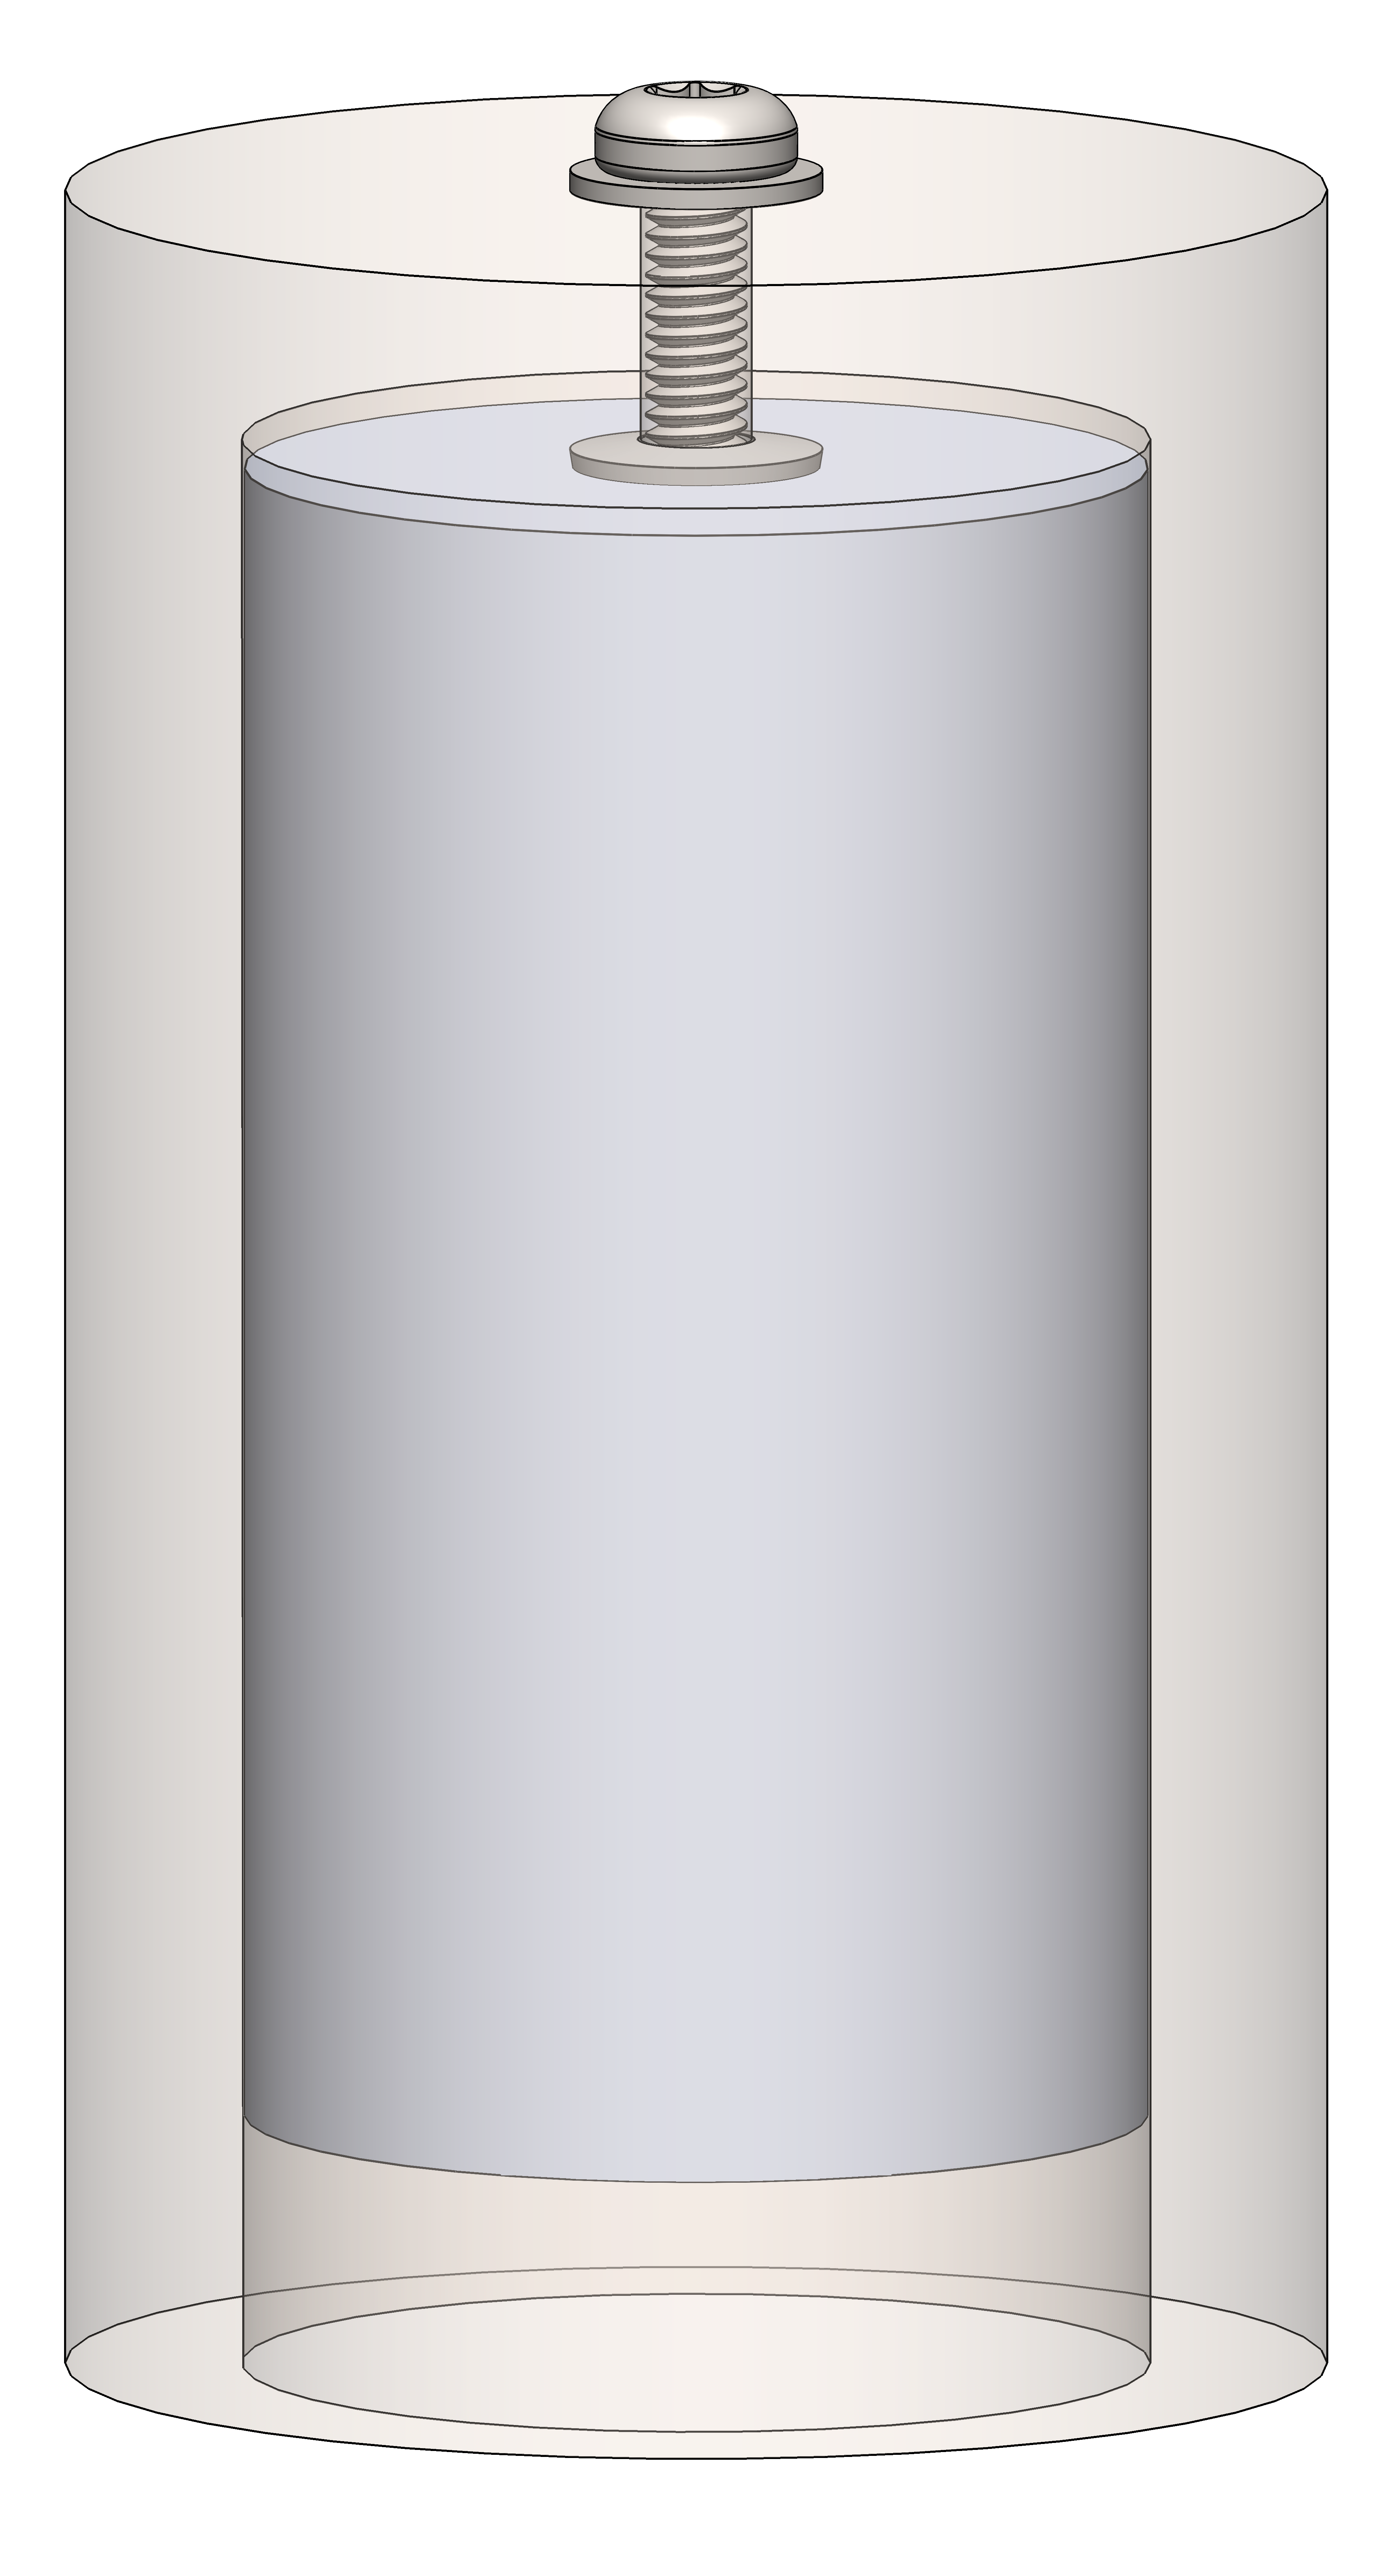
\includegraphics[height=.3\textheight, width=\textwidth, keepaspectratio]{Act_full_qual.png}
					\caption{Actuator subsystem}
					\label{fig:act_full}
				\end{minipage}
				\hfill
				\begin{minipage}{.29\textwidth}
					\centering
					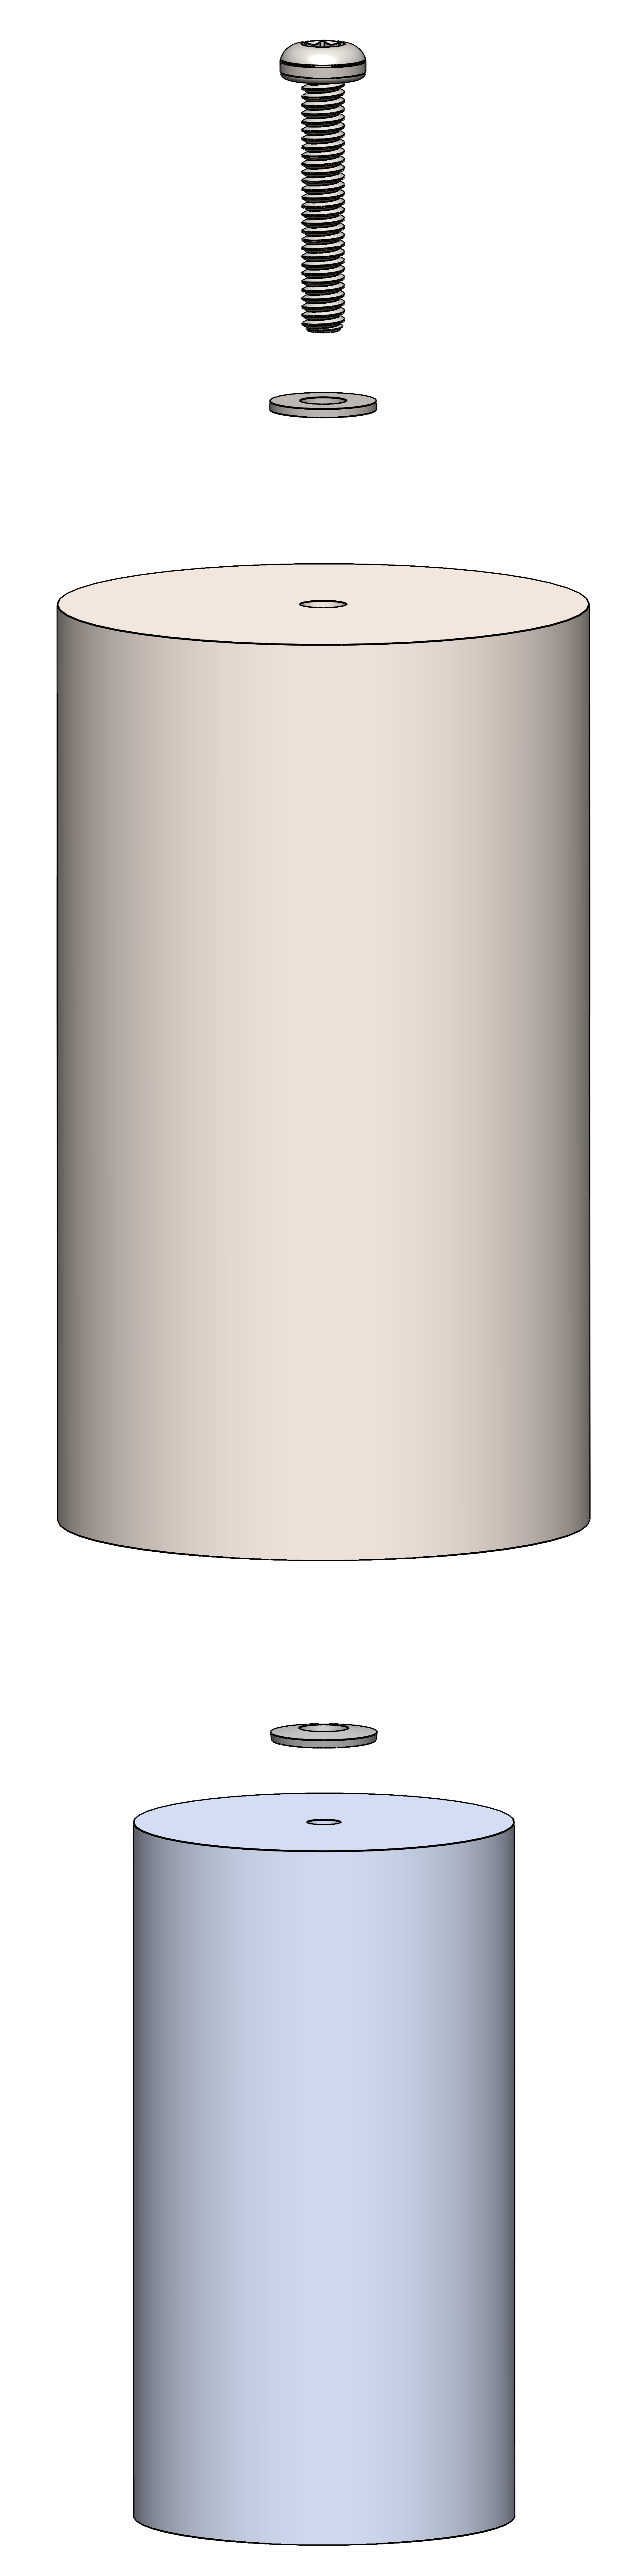
\includegraphics[height=.3\textheight, width=\textwidth, keepaspectratio]{Act_exploded_qual.png}
					\caption{Actuator subsystem exploded view}
					\label{fig:act_exploded}
				\end{minipage}
				\hfill
				\begin{minipage}{.29\textwidth}
					\centering
					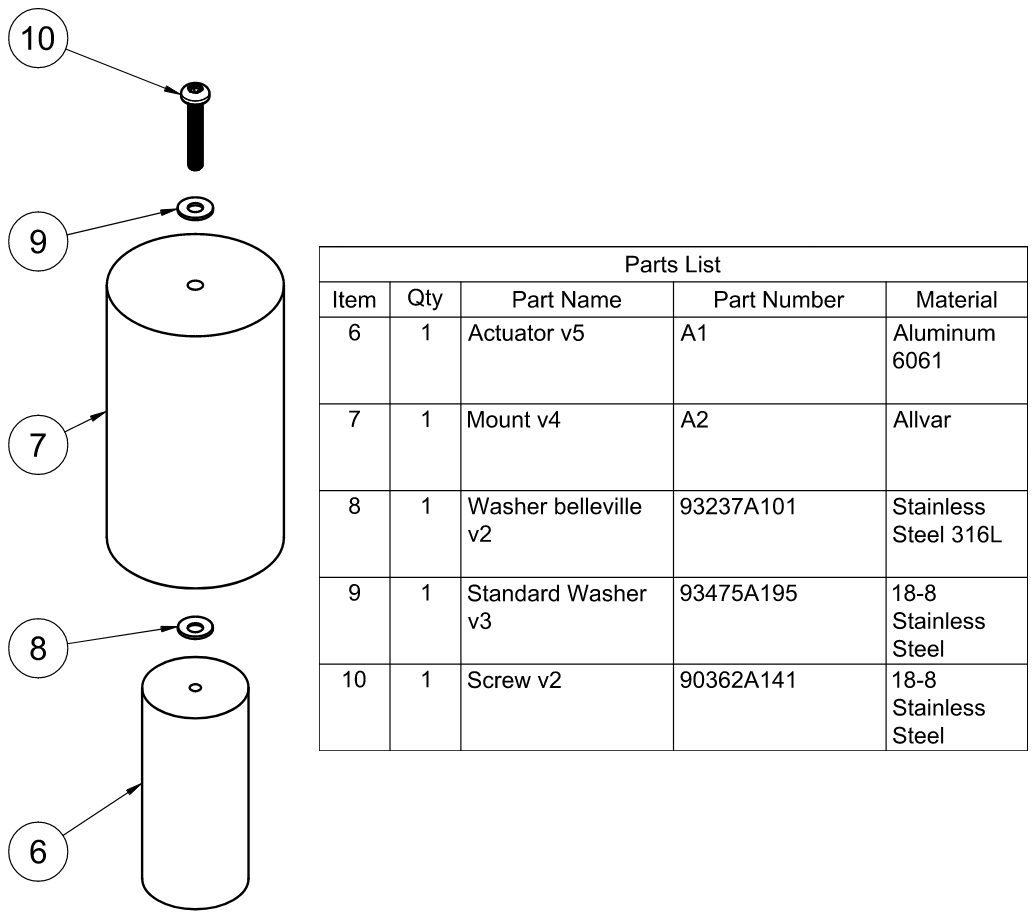
\includegraphics[height=.3\textheight, width=\textwidth, keepaspectratio]{Act_ID.png}
					\caption{Actuator subsystem part identification}
					\label{fig:act_ID}
				\end{minipage}
			\end{figure}


			The central aluminum expansion rod (6, aka the ``actuator''\footnote{
				Note that the actuator (A1 in the drawings in Appendix~\ref{app:drawings}) would best be named distinctly from its corresponding subsystem.
				This is a legacy convention from earlier stages in the design process when the mount was a distinct subsystem.
			}) nests inside an ALLVAR mount (7), suspended by the screw-washer assembly (8, 9, 10).
			The base of the mount is electron-beam welded to the top of the valve housing.
			The assembly is centered about the valve stem, which protrudes through the housing and is welded to the base of the expansion rod.
			This connection is shown in Figure~\ref{fig:Act_cut}.
			\vspace{1\baselineskip}
			\begin{figure}[H]
				\centering
				% 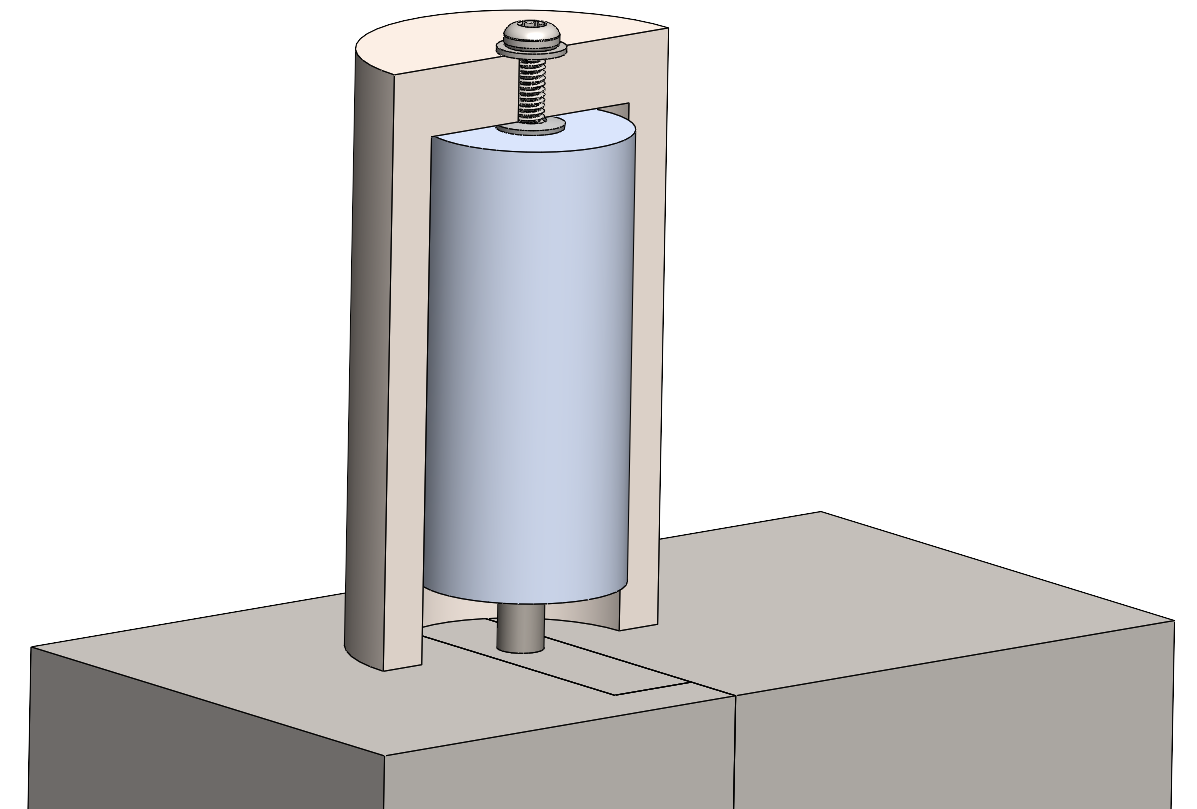
\includegraphics[width=\textwidth]{Act_cut.png}
				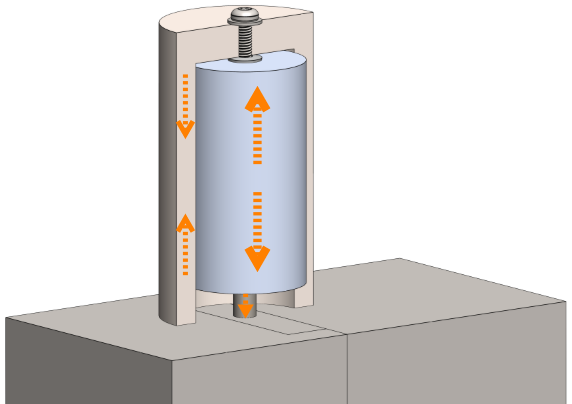
\includegraphics[width=.6\textwidth]{Act_cut_qual.png}
				\caption{Actuator-valve interface}
				\label{fig:Act_cut}
			\end{figure}

			The actuator drives the valve stem motion.
			Aluminum's coefficient of thermal expansion (CTE) is significantly higher than that of Invar 36, causing the expansion rod to expand relative to the rest of the assembly when heated.
			ALLVAR, a proprietary alloy manufactured by ALLVAR Alloys, shrinks when heated even faster than the aluminum expands.
			Because the actuator is mounted from the top, this bimetallic actuator produces more compound displacement than either metal would on its own.
			As the ambient temperature rises, the ALLVAR mount shrinks, lowering the expansion rod from above;
			this, in turn, expands downwards, driving the valve stem and closing the orifice.
			As the temperature decreases, the components reverse direction:
			the mount expands, lifting the expansion rod, which shrinks and lifts the valve stem to open the orifice.

			The expansion rod is thermally separated from the internal gas by a \SI{5}{\milli\meter} gap. Heat transfer must be minimized from this gas, which will be up to \SI{20}{\degreeCelsius} hotter than the outside air.
			Some heat will still transfer, altering the perceived ambient temperature and introducing error into the system,
			but the thick housing wall, minimal contact between subsystems, and continual free convection with the atmosphere will minimize this error.

			Small machining and assembly errors may introduce a constant offset. For instance, if the valve stem is over-dimensioned by \SI{10}{\micro\meter},
			the orifice height will be \SI{10}{\micro\meter} too high at all times, adding a constant \SI{8}{\micro\meter} to the effective diameter\footnote{as calculated in Appendix~\ref{app:calcs:orifice_geometry}}.
			Even this deviation is significant relative to its \SIrange{10}{20}{\micro\meter} tolerance window,
			illustrating the necessity to minimize independent components.
			To counter this potential constant error, the actuator subsystem includes a calibration stack.
			As the assemblers tighten the screw, fastening the expansion rod inside the mount,
			the belleville washer between them compresses. This maintains consistent tension in the screw as the relative positions of the two cylinders are tuned.

			The complete Bill of Materials and Engineering Drawings for the \device\ can be found in Appendix \ref{app:BOM} and \ref{app:drawings}, respectively.
			Appendix~\ref{app:calcs:sup:assem} shows some additional useful images of the complete assembly.
			Table~\ref{tab:part_num} summarizes the part numbers for each component of the \device, which will be used for reference in the following sections.

			\begin{table}[H]
				\centering
				\caption{Component Part Numbers}
				\label{tab:part_num}
				\renewcommand{\arraystretch}{1.3}
				\begin{tabular}{
					>{\centering\arraybackslash}p{0.08\textwidth}
					>{\raggedright\arraybackslash}p{0.22\textwidth}
					>{\centering\arraybackslash}p{0.18\textwidth}
					>{\raggedright\arraybackslash}p{0.22\textwidth}
				}
				\toprule
				\textbf{Item} & \textbf{Part Name} & \textbf{Part Number} & \textbf{Material} \\
				\midrule
				\multicolumn{4}{l}{\textit{Valve Sub-Assembly (V0)}} \\
				\midrule
				1 & Housing Inlet  & V2              & Invar 36     \\
				2 & Housing Center & V1              & Invar 36     \\
				3 & Housing Outlet & V3              & Invar 36     \\
				4 & Valve Orifice  & V4              & Invar 36     \\
				5 & Bellows        & I718-159-72-430 & Inconel 718  \\
				\midrule
				\multicolumn{4}{l}{\textit{Actuator Sub-Assembly (A0)}} \\
				\midrule
				6  & Actuator          & A1        & 6061 Aluminum        \\
				7  & Mount             & A2        & ALLVAR 30            \\
				8  & Belleville Washer & 93237A101 & Stainless Steel 316L \\
				9  & Standard Washer   & 93475A195 & 18-8 Stainless Steel \\
				10 & Screw             & 90362A141 & 18-8 Stainless Steel \\
				\bottomrule
				\end{tabular}
			\end{table}

	\section{Design Justification}
	\label{sec:design:just}

		\subsection{Transfer Functions and Critical Dimensions}
		\label{subsec:design:just:TF}

			Specifications \specref{V.1.1} and \specref{A.1.1} require specific input-output relationships to satisfy system requirement \specref{R.1}, the Required Relationship:

			\RRfull

			These values are driven by the geometry described above and by the dimensions we select for each part.

			\newpage%
			\begin{multicols}{2}
				\begin{figure}[H]
						\centering
						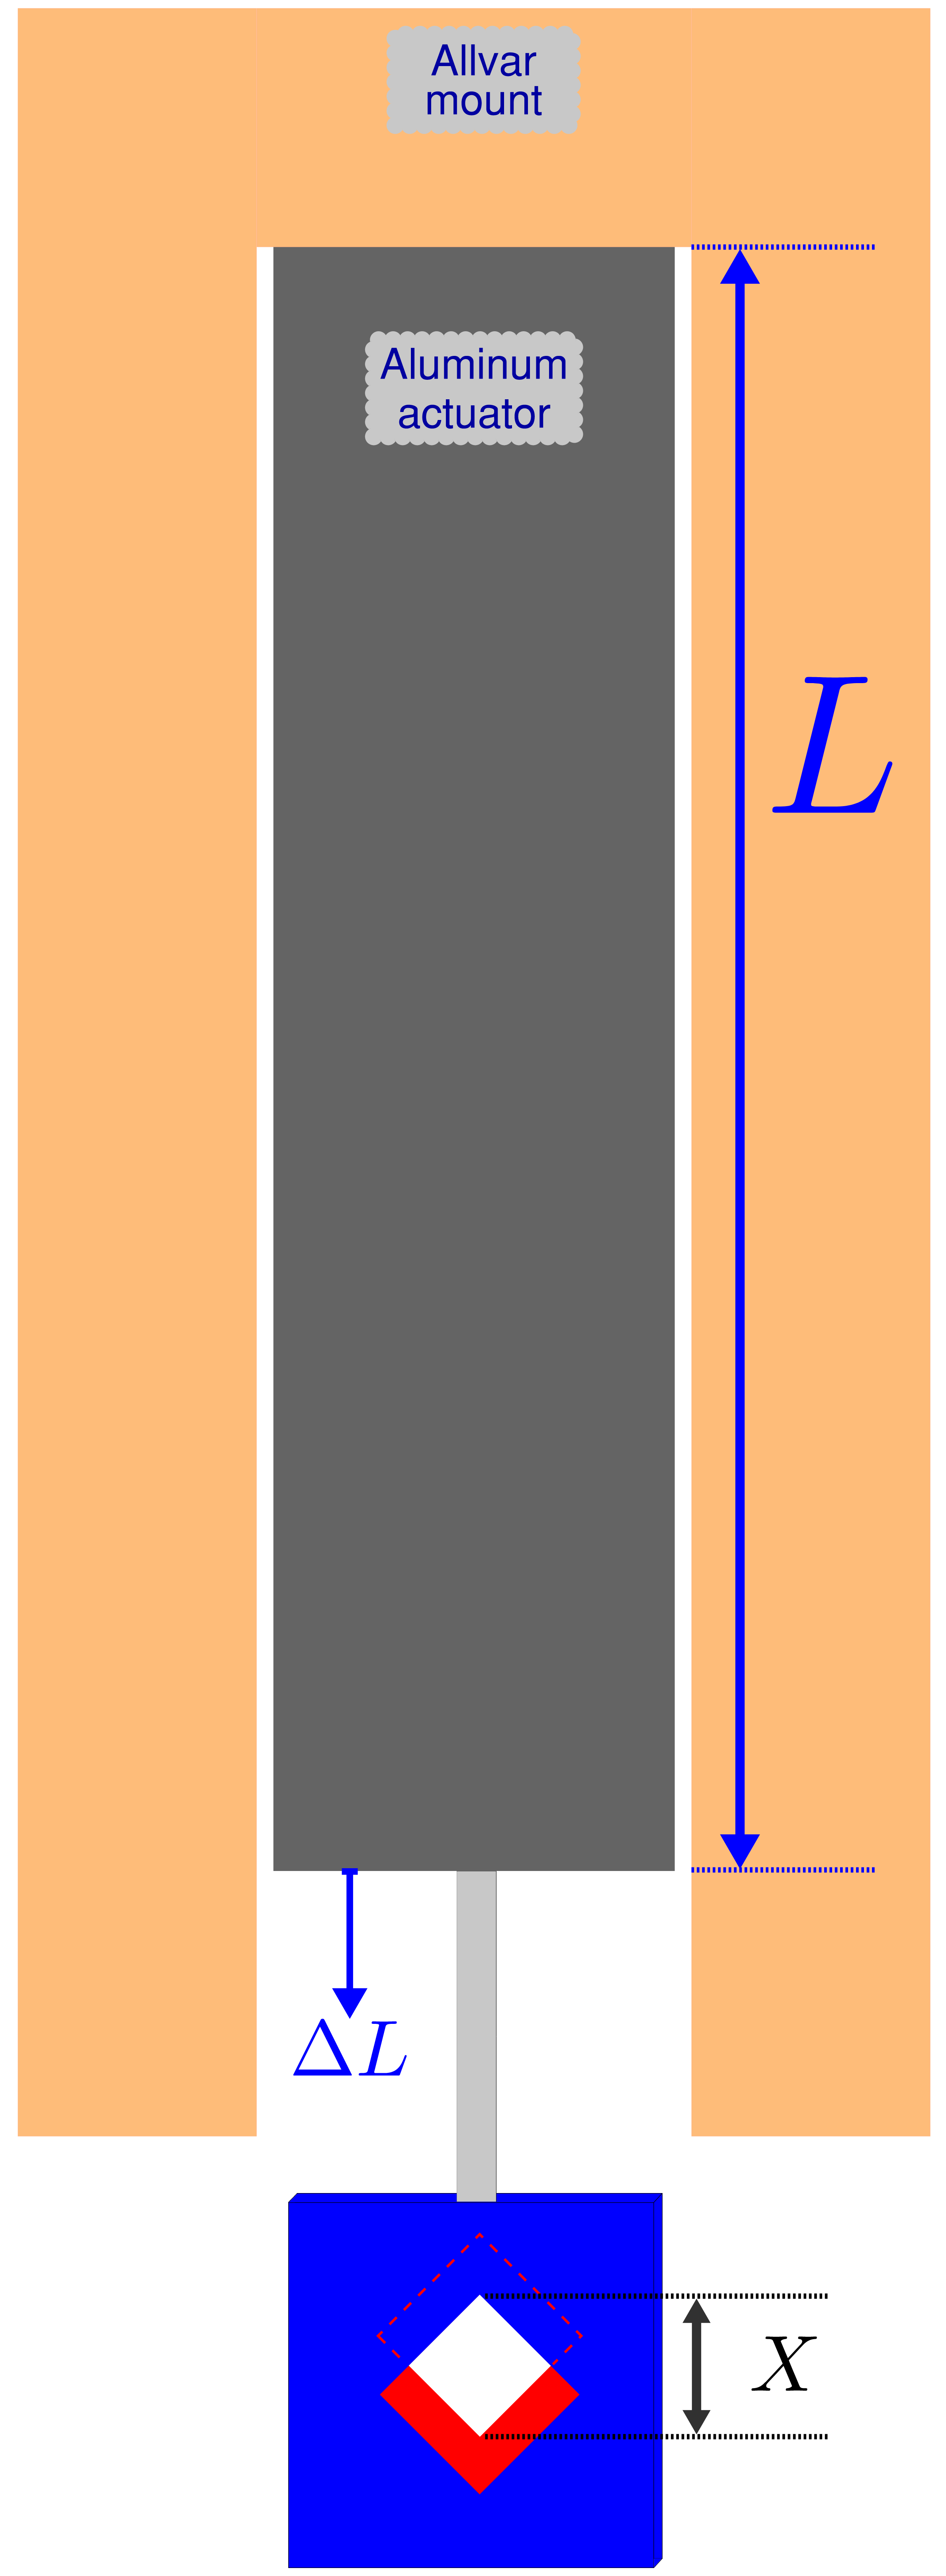
\includegraphics[height=.6\textheight]{L_X.png}
						\caption{Dimension definitions}
						\label{fig:L_X}
				\end{figure}
			\newcolumn
				Let us define the change in the actuator length, $\Delta L$, as the vertical extension of the aluminum expansion rod, which includes any rigid-body motion driven by the mount.
				See Figure~\ref{fig:L_X}. Thus, if the mount shrinks, and the expansion rod grows, by \SI{1}{\micro\meter} each, the length $L$ will increase by \SI{2}{\micro\meter}.
				This drives the valve stem an equal amount, lowering the valve stem and shrinking the orifice height $X$ by \SI{2}{\micro\meter}.

			\subsubsection{Valve Transfer Function}
			\label{subsubsec:design:just:TF:valve}

				The valve orifice geometry governs the transfer function

				\begin{equation*}
					\hat{G}_{V_0} = \frac{dD}{dL} = \frac{dD}{dX} \frac{dX}{dL}
				\end{equation*}

				that translates the change in the actuator's length, $L$\footnote{
					Note that the actuator movement may more readily be defined as the distance between the base of the mount and the base of the actuator, which in fact decreases as $L$ increases.
					The actuator length is also a legacy parameter from when the design featured a rigid Invar mount and only the expansion rod moved.},
				to a change in the effective diameter $D$.
				The orifice diameter is most readily defined by the vertical distance $X$ between its upper and lower vertices.
				As derived in Appendix~\ref{app:calcs:orifice_geometry}, the effective diameter of this orifice scales with the height by a constant factor such that

				\begin{equation}
					D_{eff} = \sqrt{\frac{2}{\pi}} X
				\end{equation}

				therefore

				\begin{equation}
					\frac{dD}{dX} = \sqrt{\frac{2}{\pi}}
				\end{equation}

				\end{multicols}

				The orifice shrinks as the actuator expands, yielding the second control derivative

				\begin{equation}
					\frac{dX}{dL} = -1
				\end{equation}

				Therefore, multiplying these together, we find

				\begin{equation}
					\hat{G}_{V_0} = -\sqrt{\frac{2}{\pi}} = \GV
				\end{equation}

				as prescribed.

				The valve subsystem also controls the reference orifice diameter $D_{ref}$.
				We can find this by calculating the orifice height at $T_{ref}$.
				According to dimensions from the engineering drawings in Appendix~\ref{app:drawings}, the top corner of the leading orifice lies

				\begin{equation*}
					\SI{40.201}{\milli\meter} - \SI{5}{\milli\meter} = \SI{35.201}{\milli\meter}
				\end{equation*}

				below the top surface of the housing, including a \SI{5}{\milli\meter} gap between that and the valve stem-actuator interface at this temperature.
				The bottom corner of the trailing orifice lies $\SI{35.519}{\milli\meter}$ below the same surface, resulting in an effective diameter of

				\begin{equation}
					D_{ref} = \sqrt{\frac{2}{\pi}} X_{ref} = \sqrt{\frac{2}{\pi}} (\SI{35.519}{\milli\meter} - \SI{35.201}{\milli\meter}) = \AzeroExact
					\label{eq:Dref}
				\end{equation}

				as specified.

			\subsubsection{Actuator Transfer Function}
			\label{subsubsec:design:just:TF:act}

			The bimetallic actuator expands at a constant rate with temperature, governing the transfer function
			
			\begin{equation*}
				\hat{G}_{A_0} = \frac{dL}{dT}
			\end{equation*}
			
			that translates the ambient temperature into motion.
			The length of each of its components drives that expansion rate. Its dimensions are shown in greater detail in Figure~\ref{fig:act_dim}.
			A belleville washer is compressed between the upper interior of the mount and the top surface of the actuator, held in place by the screw. Uncompressed, it measures \SI{0.6}{\milli\meter} tall;
			we will assume a compressed height of \SI{0.55}{\milli\meter}\footnote{
				The exact compression height of the belleville washer is, by nature, an unknown and varies between each device.
				Deviations will be accounted for in Chapter~\ref{chap:DFMEA}.}.
			A \SI{5}{\milli\meter} gap, spanned by the valve stem, separates the free end of the actuator from the housing, thermally insulating the actuator from direct heat transfer with the hot internal gas.

			\begin{wrapfigure}{l}{0.49\textwidth}
				\centering
				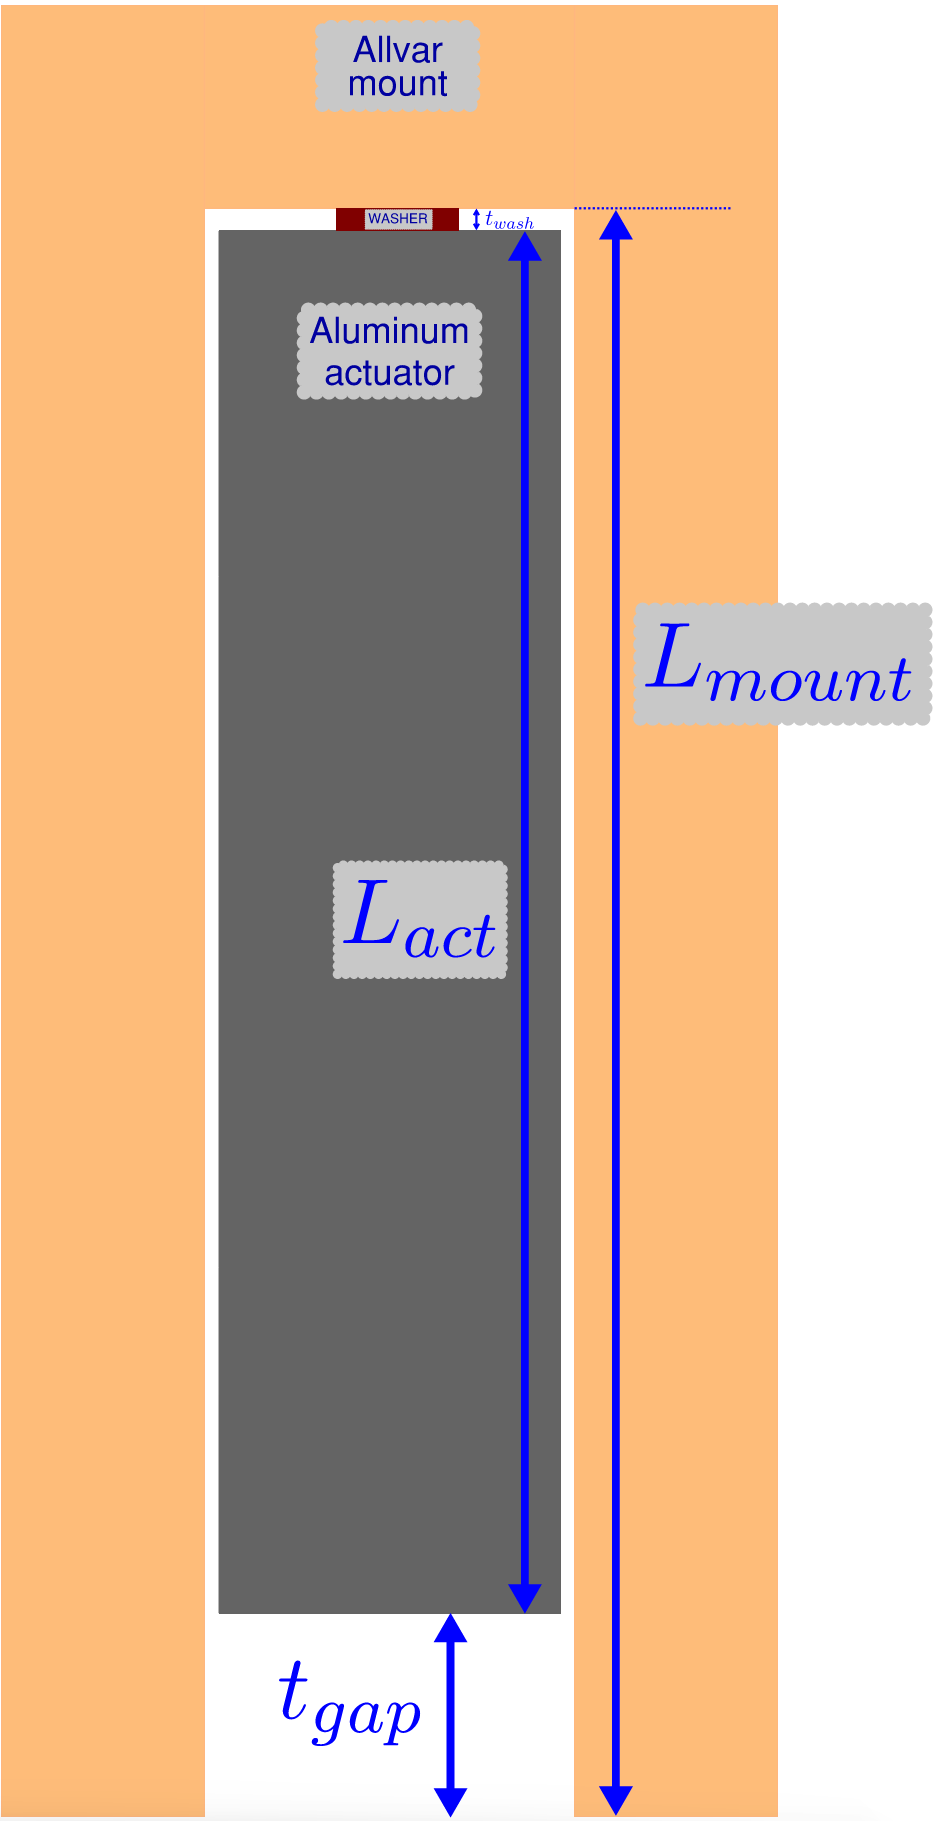
\includegraphics[width=0.47\textwidth]{Act_dim.png}
				\caption{Actuator dimension labels}
				\label{fig:act_dim}
			\end{wrapfigure}

			Assuming the base of the mount, welded to the housing, to be fixed,
			and assuming for now that the CTE of ALLVAR is positive,
			the expansion rod (aka the ``actuator'') will expand downwards as it is lifted upwards when heated. This action yields the actuation-temperature relationship in equation~\eqref{eq:actuation}.
			Because Allvar's CTE is negative, the mount will shrink as the actuator expands, aiding its action. Thus, $L_{mount} \alpha_{mount}$ increases the actuation distance $\Delta L$ by a double-negative.
			Adding the dimensions in Figure~\ref{fig:act_dim} yields the geometric relations in equation~\eqref{eq:act_dim}, giving us the following system of two equations:
			
			\begin{align}
				\Delta L = \left( L_{act} \alpha_{act} - L_{mount} \alpha_{mount} \right) \Delta T \label{eq:actuation}\\
				L_{mount} = t_{wash} + L_{act} + L_{gap} \label{eq:act_dim}
			\end{align}

			The target, from Specification \specref{A.1.1}, is

			\begin{equation}
				\frac{dL}{dT} = \frac{\Delta L}{\Delta T} = \GA
			\end{equation}

			Plugging in the following values (material properties are from Appendix~\ref{app:datasheets:mat}):

			\begin{align*}
				\alpha_{act} &= \specActuatorCTE \\
				\alpha_{mount} &= \specMountCTE \\
				t_{wash} &= \SI{0.55}{\milli\meter} \\
				L_{gap} &= \SI{5}{\milli\meter}
			\end{align*}

			we obtain the following results:

			\begin{align}
				L_{act} &= \frac{\frac{\Delta L}{\Delta T} + (t_{wash} + L_{gap}) \alpha_{mount}}{\alpha_{act} - \alpha_{mount}} \notag \\[12pt]
				&= \frac{\GA + (\SI{5.55}{\milli\meter}) \cdot (\specMountCTE)}{\specActuatorCTE - \specMountCTE} = \specOrigActuatorLength \label{eq:L_act}\\[12pt]
				L_{mount} &= L_{act} + t_{wash} + L_{gap} = \SI{38.541}{\milli\meter} \label{eq:L_mount}
			\end{align}

			These critical dimensions ensure that the actuator subsystem maintains the specified output

			\begin{equation}
				\hat{G}_{A_0} = \frac{A_1}{-\sqrt{\frac{2}{\pi}}} = \GA
			\end{equation}

			Altogether, $\hat{G}_{V_0},\ \hat{G}_{A_0}, \text{ and } D_{ref}$ combine to satisfy the functional system requirement \specref{R.1}:
			
			\begin{equation}
				\begin{aligned}
					D_{eff} &= \hat{G}_{V_0} \hat{G}_{A_0} \Delta T + D_{ref} \\
					&= \left( \GV \right) \left( \GA \right) \Delta T + \AzeroExact \\
					&= \left( \AoneExact \right) \Delta T + \AzeroExact \\
					&= A_1 \Delta T + A_0
				\end{aligned}
			\end{equation}

				This bimetallic architecture enables the actuator to be half the length of solitary high-expansion metal, keeping its total length (\SI{45.55}{\milli\meter}, accounting for the mount's upper wall and the screw that protrudes from its top) within the specified vertical mechanical envelope.

				It is useful to note that the total required motion of the actuator is

				\begin{equation}
					\Delta L = \frac{dL}{dD} \Delta D = \frac{\Delta D_{eff}}{\hat{G}_{V_0}} = \frac{D_{hot} - D_{cold}}{-\sqrt{\frac{2}{\pi}}} = \frac{\SI{170.2}{\micro\meter} - \SI{383.5}{\micro\meter}}{-\sqrt{\frac{2}{\pi}}} = \specActDefTotal
				\end{equation}

				an imperceptible motion to the human eye. The maximum deflection from the reference point is

				\begin{equation}
					\Delta L = \frac{D_{cold} - D_{ref}}{-\sqrt{\frac{2}{\pi}}} = \frac{\SI{383.5}{\micro\meter} - \SI{254.0}{\micro\meter}}{-\sqrt{\frac{2}{\pi}}} = \specActDefHot
					\label{eq:act_def_hot}
				\end{equation}

				These values will be used elsewhere to calculate conditions at the extrema.

		\subsection{Valve Architecture Selection Criteria}
		\label{subsec:design:just:geo_sel}

			To the first-time observer, the valve geometry appears peculiar and unintuitive.
			The diamond-orifice architecture was developed after serious consideration and several design iterations, described in more detail in Appendix~\ref{app:PM}.
			The following selection criteria motivated the final design of the valve orifice:

			\begin{itemize}
				\item Linearity
				\item Simplicity
				\item Direct Actuation
			\end{itemize}

			The Required Relationship stipulates that the \device\ maintain a constant temperature-diameter conversion rate, represented by the joint transfer function

			\begin{equation*}
				\hat{G}_{RR} = \hat{G}_{V_0} \hat{G}_{A_0} = A_1
			\end{equation*}

			in Section~\ref{subsec:intro:specs:RR}. $A_1$ is expressly first-order. Any nonlinear behavior in one subsystem must be either reparameterized\footnote{i.e. corrected.} in the other subsystem, an imprecise process involving a complex mechanical interface, or tolerated as error.
			$\hat{G}_{RR}$'s tolerable error is limited to 5\% of $A_1$, or \SI{76.2}{\nano\meter\per\celsius}, a razor-thin margin.
			To best reach this target, the selection process only permitted subsystem architectures that exhibit first-order behavior with minimal degrees of freedom and a direct subsystem interface.
			
			Many actuator design alternatives readily fit these criteria, as most materials maintain a linear thermal expansion rate.
			However, most valve architectures more readily translate their driving motion directly to the area of their orifice rather than its effective diameter.
			For instance, the needle valve, a reliable and precise design commonly used for gas flow control, subtracts one circle (the cross-section of its needle) from another (the hole the needle is inserted into).
			This difference causes a constant change in orifice area as the needle is moved.
			Because

			\begin{equation*}
				A \propto D_{eff}^2
			\end{equation*}

			as established in Appendix~\ref{app:calcs:orifice_geometry}, the effective diameter follows a second-order output.
			A linear relationship requires a regular orifice geometry (such as a circle, a square, or a hexagon) that maintains its shape, all sides changing at the same rate.
			Many flexible membranes required to construct a circular orifice permit hydrogen embrittlement and diffusion, disqualifying a circular geometry.
			Complex-polygon architectures, such as hexagonal camera-style aperture, comprise more degrees of freedom than the precise relationship allows.
			The diamond orifice, on the other hand, performs linearly with two interfacing components and a single degree of freedom.
			Although it was an entirely novel approach to this problem, the design fit all three selection criteria and, as demonstrated in Chapter~\ref{chap:DFMEA}, ultimately satisfies the Required Relationship.

		\subsection{Pressure Capacity}
		\label{subsec:design:just:P}

			The Invar housing, consisting of the Housing Inlet, Outlet, and two Centers, are designed and assembled to withstand \specPressure\ internal pressure without yielding according to Specification \specref{V.3.1}. 
			The Inlet and Outlet have threaded cylindrical internal geometries.
			The central cavity, which houses the internal valve components, forms a rectangular prism, all of whose sides are wetted at pressure.

			To determine the appropriate wall thickness required to sustain the internal pressure in the inlet and outlet sections, the housing is modeled as a thick-walled cylinder.
			The thickness $t$ of the housing is defined as the shortest distance from the inner wall to the outer wall.
			The following equations are used to verify structural integrity under the specified conditions.
			Since internal pressure constitutes the only significant structural load, external forces on the housing are neglected.

			\begin{table}[H]
				\centering
				\caption{Valve Housing Parameter Values}
				\label{tab:housing_parameters}
				\begin{tabularx}{\textwidth}{l X l}
					\toprule
					\textbf{Parameter} & \textbf{Description} & \textbf{Value} \\
					\midrule
					Material &
					&
					Invar 36
					\\\addlinespace
					$r_i$ &
					Inner radius &
					\SI{12.194}{\milli\meter}
					\\\addlinespace
					$t$ &
					Wall thickness (minimum) &
					\SI{7.806}{\milli\meter}
					\\\addlinespace
					$r_o$ &
					Outer radius (minimum) &
					\SI{20}{\milli\meter}
					\\\addlinespace
					$P$ &
					Internal pressure &
					$\specPressure$
					\\\addlinespace
					$S_y$ &
					Yield strength &
					\SI{276}{\mega\pascal}
					\\\bottomrule
				\end{tabularx}
			\end{table}

			The principal stresses, those along the three orthogonal axes, are as follows\cite{ref_shigley}:
			\begin{equation}
			\sigma_{\theta} = P \left( \frac{r_o^2 + r_i^2}{r_o^2 - r_i^2} \right) = 68.95 \left( \frac{20^2 + 12.194^2}{20^2 - 12.194^2} \right) \approx \SI{150.54}{\mega\pascal} \quad (\text{Hoop Stress})
			\end{equation}

			\begin{equation}
			\sigma_{r} = -P \approx \SI{-68.95}{\mega\pascal} \quad (\text{Radial Stress})
			\end{equation}

			\begin{equation}
			\sigma_{z} = P \left( \frac{r_i^2}{r_o^2 - r_i^2} \right) = 68.95 \left( \frac{12.194^2}{20^2 - 12.194^2} \right) \approx \SI{40.80}{\mega\pascal} \quad (\text{Longitudinal Stress})
			\end{equation}
			
			The housing must be designed against yield, or plastic\footnote{Irreversible.} deformation.
			Its yield strength can be readily compared against the Von Mises stress, which measures the distortion energy as a combination of the principal stresses.

			\begin{equation}
				\begin{aligned}
					\sigma_{\text{vm}} &= \sqrt{\frac{(\sigma_\theta - \sigma_r)^2 + (\sigma_r - \sigma_z)^2 + (\sigma_z - \sigma_\theta)^2}{2}} \\
					&= \sqrt{\frac{(150.54 - (-68.95))^2 + (-68.95 - 40.80)^2 + (40.80 - 150.54)^2}{2}}
				\end{aligned}
			\end{equation}

			\begin{equation}
			\approx \SI{190.08}{\mega\pascal}
			\end{equation}

			This yields a safety factor of

			\begin{equation}
			FS = \frac{S_y}{\sigma_{\text{vm}}} = \frac{276}{190.08} \approx 1.45 > 1
			\end{equation}

			verifying that the cylindrical Housing Inlet segment carries sufficient material to hold the maximum specified internal pressure.
			System pressure capacity drove the valve subsystem's lateral mechanical envelope of \SI{40}{\milli\meter},
			which is sufficiently thick to satisfy its pressure requirements and well within its size constraints.

			The above estimate is conservative and assumes a cylindrical exterior with a wall thickness equal to the thinnest dimension of the actual design.
			The rectangular housing exterior circumscribes this cylinder, providing extra strength.
			
			The housing center pieces are joined using welded connections and designed with a wall thickness of \SI{10}{\milli\meter}, which is greater than the minimum required thickness of \SI{7.806}{\milli\meter}, to ensure that the pressure boundary is maintained at the critical junction where the three sections of the housing meet.
			Because the center pieces form a rectangular prism, the stress distribution is more complex than in a cylindrical geometry, and was difficult to model analytically. However, the increased thickness of \SI{10}{\milli\meter} provides a significant safety margin to ensure that the housing center can withstand the internal pressure without failure.
			Flat-walled pressure vessel behavior and stress concentrations at the corners may, however, produce more than the critical stress;
			this risk is evaluated in more detail in Section~\ref{subsec:design:just:weld_analysis}.

		\newpage % Delete if necessary
		\subsection{Hermetic Seal}
		\label{subsec:design:just:bellows}

		\begin{wrapfigure}{l}{0.45\textwidth}
				\centering
				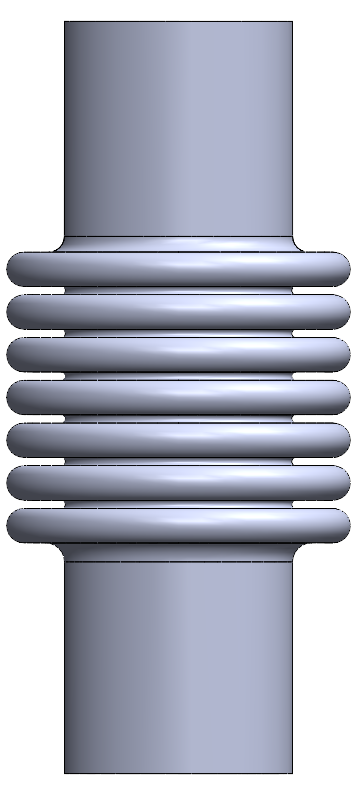
\includegraphics[width=0.35\textwidth]{bellows.png}
				\caption{CAD model of the I718-159-72-430 bellows}
				\label{fig:bellows}
		\end{wrapfigure}

		The \device\ requires mechanical penetration of a pressure vessel. Specifications \specref{V.3.2} and \specref{V.3.3} require a hermetic seal\footnote{
			Named after the Greek God Hermes\cite{ref_wilton_hermetic}, a hermetic seal limits gas leakage to nearly zero.
			It originates from the alchemetic practice of fusing glass vessels together such that air cannot escape\cite{ref_gesner_1559}.
		} to prevent leakage through this interface.
		Typical polymer gaskets permit hydrogen diffusion and are subsequently embrittled, significantly limiting the lifetime of the seal.
		Hydrogen gas molecules, the smallest in existence, seep through the long polymer chain structures with ease, spurred by an enormous back pressure, and react with the polymer material.
		Flexible metal bellows bypass this concern with a hermetic seal that is directly fused between the valve stem and the housing structure.
		The flexible tube comprises convolutions that stretch and compress with little resistance when driven axially but can withstand substantial radial pressure loads.
		The I718-159-72-430, pictured in Figure~\ref{fig:bellows}, can hold a seal at pressures up to \specBellowsBurst.
		At the maximum deflection (c.f. eq.~\eqref{eq:act_def_hot}), both bellows exert a maximum force\cite{ref_Young_Freedman, ref_miniflex_catalog} of

		\begin{equation}
			F = 2 k \Delta L = (2) \left(\specBellowsK \right) \left(\specActDefHot \right) = \SI{24}{\newton}
			\label{eq:bellow_F}
		\end{equation}

		The lower valve stem connects to nothing. It and the second bellows could easily be discarded.
		However, because the whole Valve Orifice (the moving component) is surrounded by high-pressure gas, doing so would create a force imbalance.
		Every pressure force on one side of the part is balanced by an equivalent force on the opposite side except for the area sealed by the top bellows,
		inside of which is air at atmospheric pressure.
		The corresponding area under the valve orifice would take unequilibrated pressure, causing a net upwards force of

		\begin{equation}
			\begin{aligned}
				F &= P A = (\textit{internal pressure}) \left( \frac{\pi}{4} (\textit{Neck 1 OD})^{\footnotemark} \right) \\
				& = (\specPressure) \left( \frac{\pi}{4} (\SI{4.09}{\milli\meter})^2 \right) = \SI{906}{\newton}
			\end{aligned}
		\end{equation}
		\footnotetext{The smaller of the bellows' two necks\cite{ref_miniflex_catalog}, which is connected to the Valve Orifice.}

		The second bellows adds \SI{24}{\newton} to remove \SI{906}{\newton}.

		The bellows drove many of the surrounding dimensions and features.
		According to the manufacturer's Design Guide, the burst pressure assumes that the bellows is ``restrained from squirm or sideways movement'' such that ``squirm will not occur if the bellows is guided internally\ldots\ by a rod or stem''\cite{ref_miniflex_design}.
		The valve stem, which passes through the bellows, measures just smaller than the bellows convolution inner diameter (\specBellowsID) to provide support against squirm (i.e. pressure-driven lateral buckling).
		The housing inlet allows just enough space to fit the bellows, minimizing waste. Regardless, the housing inlet exceeds its specified mechanical envelope to accommodate the two long bellows.
		This violation is justified in Section~\ref{subsubsec:design:just:gen_dim:ME}.


		\subsection{Calibration}
		\label{subsec:design:just:cal}

			Slight machining errors in every dimension will be present. Even those within their specified tolerance can endanger the system performance of the \device.
			Deviation from the intended thermal expansion rate cannot be adjusted post-manufacture, but any constant offset, such as from extra length in the valve stem, can be.
			The calibration stack, pictured in Figure~\ref{fig:cal}, allows the user to set the output of the device at a single temperature, shifting the whole system output closer to the center of its tolerance in satisfaction of Specification \specref{A.1.2}.
			The actuator subsystem is assembled and fastened using an M2 screw, which passes through the mount, supported by a flat washer, and threads into the central expansion rod.
			As the screw is tightened, a belleville washer between the two clamped faces maintains tension in the screw, letting the threads seat at any position within the belleville washer's range.
			See Appendix~\ref{app:calcs:cal:force} for further calculations and Appendix~\ref{app:mfg} for calibration instructions.
			Calibration ought to be performed at room temperature (approximately $T_{ref}$), where the required tolerance window is narrowest (c.f. Appendix~\ref{app:calcs:orifice_geometry}).
			\vspace{1\baselineskip}
			\begin{figure}[H]
				\centering
				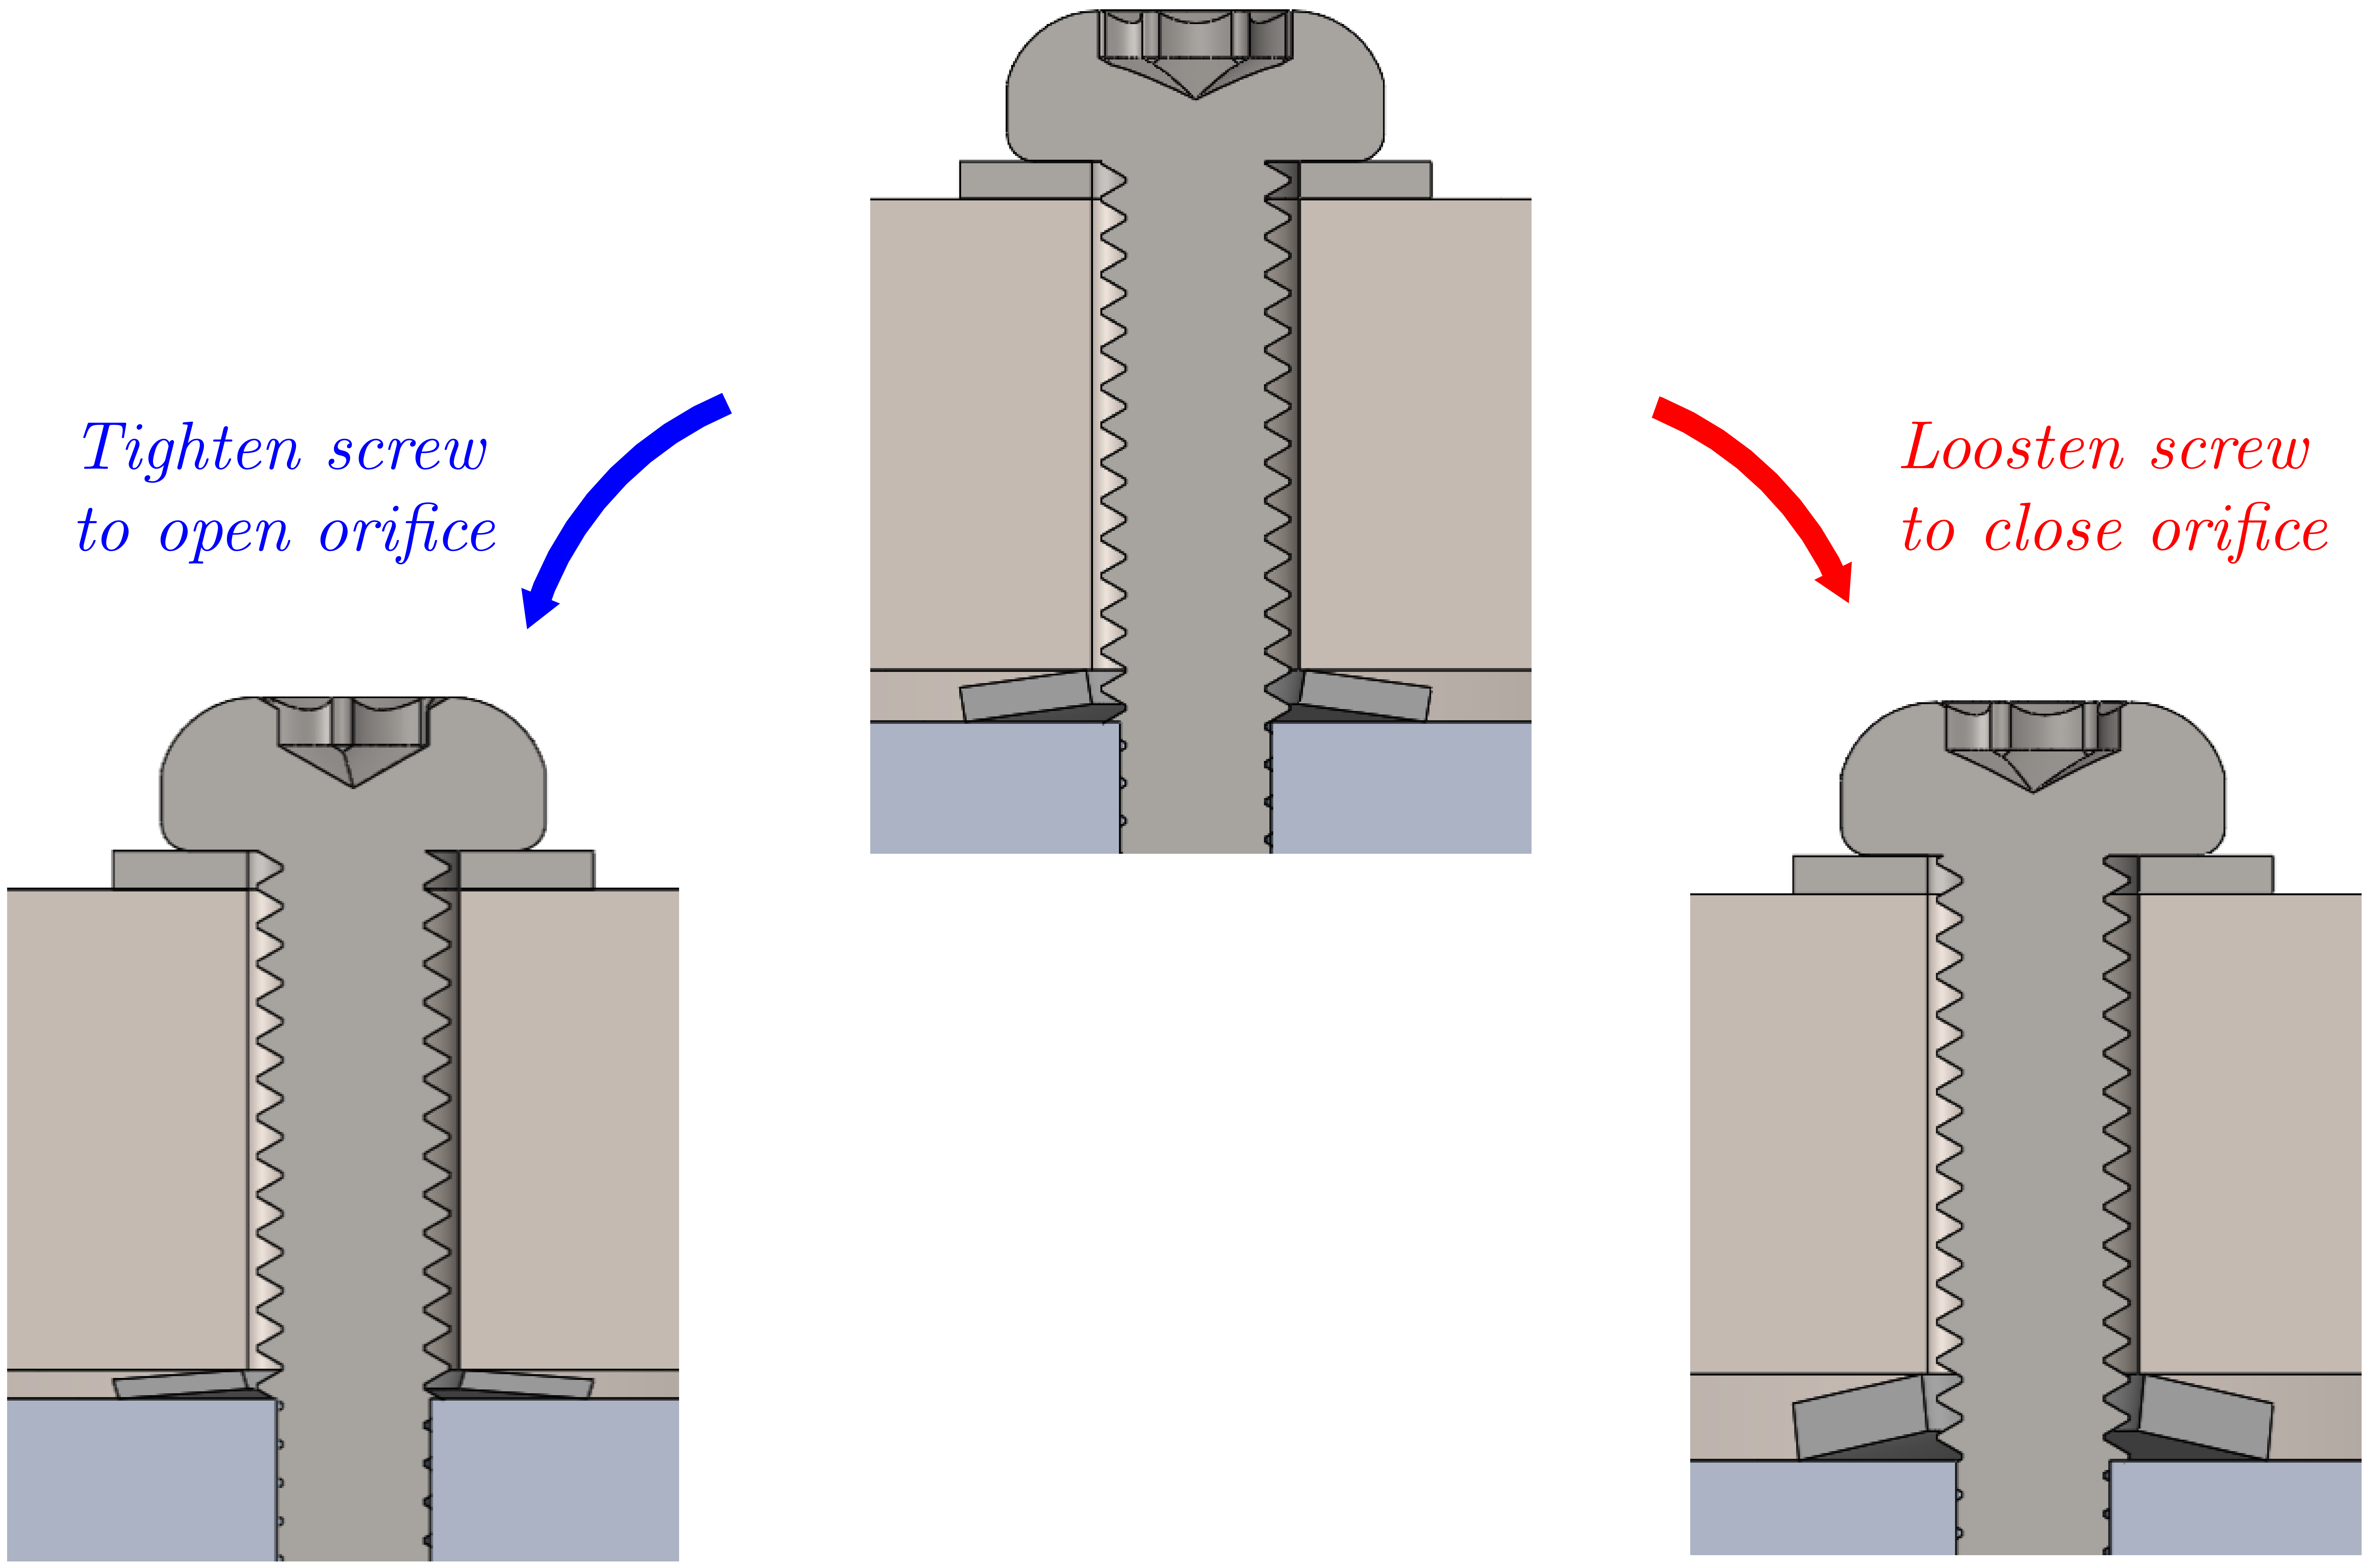
\includegraphics[width=.5\textwidth]{cal.png}
				\caption{System Calibration with a belleville washer}
				\label{fig:cal}
			\end{figure}

		\subsection{Weld Joint Overview}
		\label{subsec:design:just:weld_overview}

		The \device\ is assembled using Electron Beam Welding (EBW), a high-precision welding 
		technique that uses a focused beam of electrons to join materials 
		together\cite{ref_steen2010laser}. EBW was selected for several reasons critical to 
		the \device's performance requirements. First, welding the entire assembly eliminates 
		mechanical fasteners and threaded interfaces, minimizing the degrees of freedom in the 
		final assembly and preventing the backlash and compliance introduced by alternative 
		joining methods. This directly improves system-level positioning precision, which is 
		essential given the tight tolerances required at the valve orifice. Second, EBW's high 
		power density enables complete fusion across the interface in a single pass, producing 
		full-penetration welds with a narrow heat-affected zone and minimal thermal distortion.
		This is critical for maintaining the dimensional tolerances of the precision fits 
		described in Section~\ref{subsec:design:just:fits}.

		The \device\ requires five different types of welds:

		\begin{itemize}
			\item Circumferential welds joining the bellows to the housing centers and the 
				valve orifice.
			\item Orthogonal welds joining the housing centers to the housing inlet.
			\item A circumferential weld joining the housing inlet and center pieces to the 
				housing outlet.
			\item A weld joining the actuator to the valve stem.
			\item A circumferential weld joining the mount to the housing.
		\end{itemize}

		Of these, the welds joining the housing inlet, outlet, and center pieces are the most 
		critical, as they form the pressure boundary of the valve and are subject to the highest 
		stresses. These joints use a square butt geometry, which is widely used in pressure 
		vessel construction and permits full penetration by EBW. Full penetration is considered 
		achieved when the weld fuses through the entire wall thickness $t$.

		Weld quality is verified using 100\% X-ray radiographic inspection per ASME 
		B31.3\cite[Table~302.3.4]{ref_asme_b313}. With all welds passing inspection 
		($E = 1.00$), no strength penalty relative to the base material is introduced, and the 
		joints are certified free of defects such as porosity, lack of fusion, and cracking, 
		all of which could significantly reduce joint strength\cite{ref_steen2010laser}. The 
		structural adequacy of the critical pressure-boundary welds is evaluated in 
		Section~\ref{subsec:design:just:weld_analysis}.

		\subsection{Precision Fits}
		\label{subsec:design:just:fits}

			The \device\ features several components that will slide closely against one another, either once during assembly or repeatedly during operation.
			The tolerances of the inner and outer component, which are referred to as the ``shaft'' and ``hole'' (though not always circular), can be optimized according to the application's precision-friction trade-off. 
			Shigley's Mechanical Engineering Design\cite[Tables 7-9, A-11, A-12]{ref_shigley} establishes best practice for fit tolerances by fine-tuning the maximum and minimum tolerances of each hole and shaft dimension.
			For each of the following fits, the necessary balance between locational precision and frictionless movement yielded a particular fit type, which corresponds to a given code (e.g. H7/g6) for use in the engineering drawings.

			\begin{itemize}
				\item The actuator slides against the mount as it expands. To minimize deflection (see Section~\ref{subsubsec:design:just:gen_dim:act_diam}), the internal expansion rod should fully span the mount's bore diameter.
					However, sufficient clearance will ensure that their surfaces do not touch, especially as each expands laterally\footnote{ALLVAR is not isotropic. This means that although its vertical CTE is negative, its horizontal CTE values are positive like any ordinary metal. Thus, both components of the actuator will expand as they heat, building friction at their contact surfaces if not given sufficient clearance.}
					with temperature. A \textit{free running fit} (H9/d9) provides sufficient accuracy with enough clearance to avoid any friction.
				\item The valve stem must be machined to the bellows' exact convolution inner diameter to support it against pressure-driven squirm (see Section~\ref{subsec:design:just:bellows}), but like the actuator, contact should be avoided.
					Because Inconel and Invar expand far less than aluminum and ALLVAR, a closer fit can be afforded to prevent lateral movement.
					A \textit{sliding fit} (H7/g6) allows for low-friction movement at low speeds; it is the closest fit before contact occurs.
					While the bellows convolution inner diameter tolerance cannot be manipulated, a g6 tolerance on the valve stem will ensure minimal friction.
					Likewise, the hole in the housing center guides the valve stem's motion and requires the same tolerance (H7).
				\item The valve stem's lateral placement critically affects the orifice geometry; its fit must permit minimal side-to-side movement. However, as with the valve stem, a snug fit risks galling (see Section~\ref{subsubsec:design:just:gen_dim:friction}), which would allow for a buildup of static friction before movement occurs,
					so another \textit{sliding fit} (H7/g6) ensures free locational motion while maintaining light contact on all sides.
				\item The housing center should be snugly seated into the housing inlet upon assembly.
					After it is welded in place, friction will be irrelevant; thus, to locate the housing center's hole as precisely as necessary, a \textit{locational clearance fit} (H7/h6) will be applied.
			\end{itemize}

		\subsection{Material Selection}
		\label{subsec:design:just:mat}

		
			Each material selected for the \device\ enabled its exceptional performance despite impossible design circumstances.
			The Ashby Chart\cite{ref_ashby} (Figure~\ref{fig:ashby}), an engineering standard for thermal stress of materials, provides a fitting guide for the relative strength and thermal expansivity of various metals, polymers, and ceramics.
			Materials further up and to the right will possess greater driving authority when expanding, either by a higher CTE $\alpha$ or higher stiffness $E$.
			
			\begin{figure}[h]
				\centering
				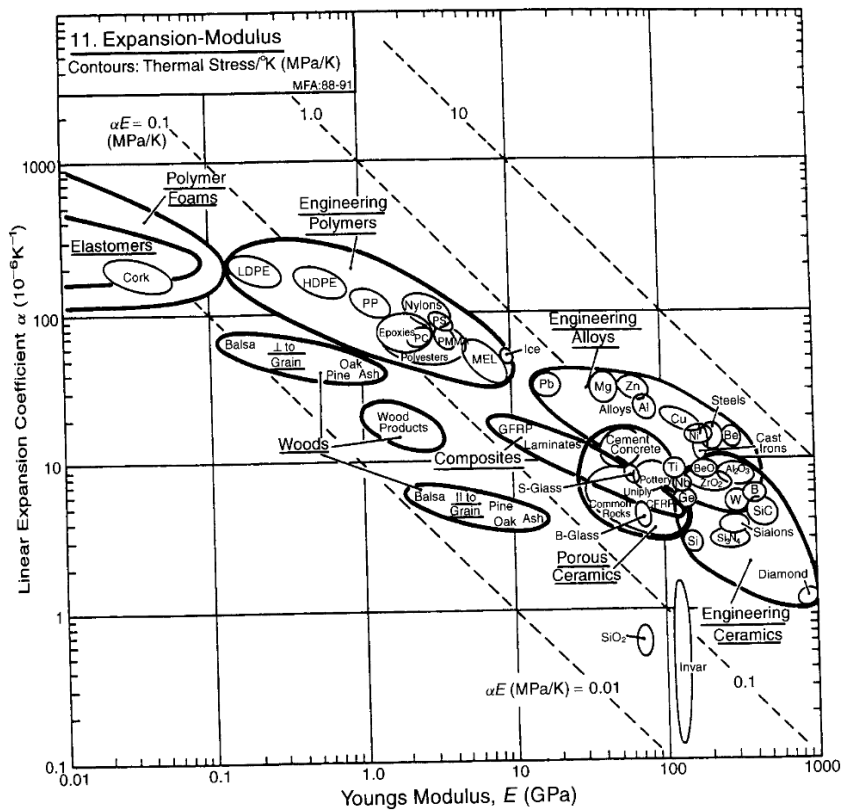
\includegraphics[width=.75\textwidth]{ashby.png}
				\caption{The Ashby Chart for Metals, Polymers, and Ceramics}
				\label{fig:ashby}
			\end{figure}
			
			\subsubsection{Aluminum expansion rod}
			\label{subsubsec:design:just:mat:Al}

				The actuator expansion rod requires a high, stable thermal expansion rate to properly drive the valve stem.
				As reflected on the Ashby Chart, polymers possess the highest CTE, but they are soft (meaning they will readily deflect under reaction forces, such as from the bellows) and exhibit an inconsistent expansion rate across the full design temperature range.
				Ceramics, though they have a high thermal stiffness, will hardly expand due to their low CTE, and their high modulus of elasticity makes them nearly impossible to machine to the necessary tolerance.
				Some metals, such as certain Zinc and Magnesium alloys, have a CTE as high as \SI{30}{\micro\meter\per\meter\per\celsius}, but like the polymers, their expansion rates are too inconsistent for the precise output required by the \device.
				Aluminum\cite{ref_NASA_specs_Al} stands alone\footnote{
					This absolute must be taken with a grain of salt. While ALLVAR, Invar 36, and Inconel 718 show strong evidence that they are the best material choices for their respective applications, aluminum may be best replaced with a certain Zinc or Magnesium alloy.
					Its selection process was expedited due to time constraints. Further research may reveal an alloy with a consistent CTE higher than that of aluminum, allowing for a shorter bimetallic actuator.} 
				as a strong, expansive, consistent metal. It has a CTE of \specActuatorCTE\ at $T_{ref}$ that varies a maximum of \SI{1}{\micro\meter\per\meter\per\celsius} as $\SI{-60}{\celsius} \leq T_{amb} \leq \SI{80}{\celsius}$.

			\newpage
			\subsubsection{Allvar mount}
			\label{subsubsec:design:just:mat:ALLV}

				\begin{wrapfigure}{l}{.45\textwidth}
					\centering
					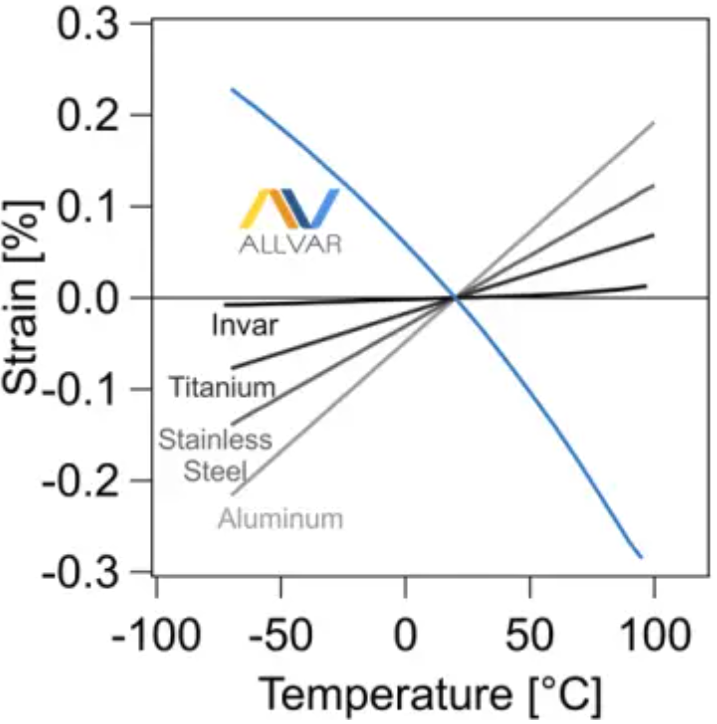
\includegraphics[width=.43\textwidth]{ALLVAR_CTE.png}
					\caption{CTE of ALLVAR against other metals}
					\label{fig:ALLVAR_CTE}
				\end{wrapfigure}

				ALLVAR Alloy 30\cite{ref_AllvarAlloys}, used for the mount as the second actuator metal, 
				is a proprietary, Titanium-based alloy patented by ALLVAR Alloys\cite{ref_AllvarAlloys_gen}.
				Unlike any other metal, it shrinks along one axis when heated, allowing for the compact bimetallic actuator design.
				Its CTE magnitude is even higher than that of aluminum and just as consistent\footnote{Although ALLVAR Alloys does not provide temperature-dependent thermal expansion data for their products, and although their thermal expansion data presented in Figure~\ref{fig:ALLVAR_CTE} is imprecise, they claim a mostly linear expansion rate across our whole design temperature range.}
				(Figure~\ref{fig:ALLVAR_CTE}\cite{ref_AllvarAlloys}).

				Several thermal switch designs\cite{ref_Bugby_2021, ref_Ralphs_2024, ref_Ralphs_2026}, which make use of a binary-output bimetallic actuator for aerospace heat-transfer applications, have used the ALLVAR-aluminum combination\footnote{The cited papers\cite{ref_Bugby_2021, ref_Ralphs_2024, ref_Ralphs_2026} were provided to our team directly by ALLVAR Alloys in support of their technology.},
				validating this combination.

				Furthermore, ALLVAR exhibits a low coefficient of thermal conductivity $(k = 8.88)$, providing thermal resistance to heat conducted through the valve housing.

			\subsubsection{Invar housing}
			\label{subsubsec:design:just:mat:Inv}

				Invar 36\textsuperscript{{\textregistered{}}}\cite{ref_Carpenter_Inv}, used for all machined parts in the valve subsystem, exhibits an exceptionally low coefficient of thermal expansion.
				Swiss physicist and metrologist Charles \'{E}douard Guillaume unexpectedly discovered the exotic metal Invar, short for ``\textit{invariable}'', in 1897\cite{ref_Invar_1897}.
				He won a Nobel Prize for this discovery in 1920\footnote{
					The curious individual may find Guillaume's 1920 Nobel Prize lecture\cite{ref_Invar_1920} particularly fascinating.
				}\cite{ref_Invar_1920}.
				Carpenter Technology\cite{ref_Carpenter_gen}, a manufacturer of the alloy, now holds the registered trademark to the name Invar 36 and confirms that its CTE reaches no more than \specInvarCTE\ within the design temperature range\cite{ref_Carpenter_Inv},
				ten times less than that of steel\cite{ref_ASM_Steel} and 20 times less than aluminum\cite{ref_NASA_specs_Al}.
				This special property allows exceptional thermal stability in the parts not designed to expand, allowing for precise thermomechanical performance.
				The Ashby Chart (Figure~\ref{fig:ashby}) makes apparent that Invar stands alone as a low-expansion metal. Only ceramics, which are too hard to machine, approach its expansion rate.
				Invar is plotted with such an eccentric ellipse, not because its CTE is inconsistent across temperature, but because myriad heat-treatment and work-hardening processes can bring its CTE as low as \SI{0.15}{\micro\meter\per\meter\per\celsius}.
				Guillaume claimed to have brought one sample of Invar wire several kilometers long to a negative CTE, annealed it back to near-zero, and found its expansion rate imperceptible even at that length\cite[p.~452]{ref_Invar_1920}.

				Invar, like ALLVAR, resists thermal conduction $(k = 10.5)$. Heat transfer between the heated gas and the actuator subsystem is better inhibited than it would be by other metals.

			\subsubsection{Inconel bellows}
			\label{subsubsec:design:just:mat:Inc}

				INCONEL\textsuperscript{{\textregistered{}}}\cite{ref_SpecialMetals_Inc} Alloy 718, a Nickel superalloy used by Mini-Flex for their high-pressure bellows, outperforms any other metal on several key metrics as a hermetic seal and is ubiquitous in the aerospace industry\cite[p.~1]{ref_SpecialMetals_Inc}.
				Special Metals Corporation\cite{ref_SpecialMetals_gen} now holds the registered trademark\footnote{
					Inconel, like Invar, was discovered by mistake, this time by American metallurgist Herbert Louis Eiselstein for INCO in 1965\cite{ref_Inconel_1965}.
					Curious readers will find his account of the discovery (given at a metallurgy conference in 1991) compelling\cite{ref_Inconel_1991}.}.
				Its CTE and Elastic Modulus are unspectacular and near that of steel.
				Nevertheless, such conventional metals fail several criteria required to meet and maintain Specifications \specref{V.3.2} and \specref{V.3.3}:

				\begin{itemize}
					\item \textbf{Strength at temperature.} All metals soften when heated and embrittle when chilled. Inconel, according to its developer, is ``suitable for temperatures from [\SI{-250}{\celsius}] up to [\SI{700}{\celsius}]''%
						\footnote{Converted from \textdegree F}\cite[p.~62, 74--76]{ref_Inconel_1965}.
					\item \textbf{Fatigue resistance.} Metals wear under repeated cyclic loads typical of a bellows. Inconel outlasts most metals under such conditions, reported to have ``Good tensile, fatigue, creep, and rupture strength'' by its manufacturer\cite[p.~1]{ref_SpecialMetals_Inc}.
					\item \textbf{Hydrogen compatibility.} All gases diffuse (penetrate) through all metals imperceptibly. Hydrogen does this particularly aggressively, leading to embrittlement, the loss of a metal's ductility as its material reacts with the seeping gas.
						Inconel, though an imperfect barrier, is especially immune to this phenomenon. Jonathan Lee, writing for NASA in 2016\cite[Table~4]{ref_NASA_Inc}, rated Inconel 718 as ``Extreme'' on the Hydrogen Environmental Embrittlement (HEE) scale at conditions up to \SI{68.9}{\mega\pascal}.
					\item \textbf{Weldability.} Prior to the development of Inconel 718, the leading precipitation-hardened Nickel superalloys used in the industry all suffered from heat embrittlement, causing them to crack. Inconel, found to be particularly suitable for electron-beam welds, drove the alloy's industry dominance.
				\end{itemize}

				See Appendix~\ref{app:datasheets:mat} for relevant material data used throughout this report.

\chapter{Model Verification}
\label{chap:DFMEA}

\section{Introduction to Failure Mode Effect Analysis and Methods}
\label{sec:DFMEA:FMEA}
	The high performance requirements and extreme operating conditions of this device require in-depth risk assessment via Design Failure Mode Effect Analysis (DFMEA). Possible failure modes are identified
	and ranked  by Risk Priority Number (RPN) according to their effect on precision and function of the PTCD as a whole. RPNs are calculated for each failure mode
	by taking the product of the qualitative ranking of individual factors of failure severity, probability of occurrence, and ease of detection. A critical RPN
	of 100 was chosen to be the threshold for in-depth analysis and potential redesign. Note that these failure modes were identified and ranked through preliminary calculations
	and are verified or challenged by theoretical modeling in Chapter~\ref{chap:test}.


\begin{figure}[h]
                \centering
                
\includegraphics[width=\textwidth]{ DFMEA_table_priority_modes.png}
                \caption{Prioritized Failure Modes with RPN>120}
                \label{fig:RPN_priority}
            \end{figure}

	The threshold RPN was chosen to be 100. The main failure risks 
	device inaccuracy, loss of function, and damage to the PTCD and nearby equipment at the worst case.
	This RPN value was deemed the critical point at which these would prove the device incapable of performing within an acceptable
	tolerance range.
	Each of the critical failure modes identified must undergo analytical and computational testing to confirm reliability and performance of the current PTCD design, or to 
	inform suggestions for redesign and modification. The results of computational modeling are discussed in Chapter~\ref{chap:test}.

	\section{Weld Failure Analysis}
	\label{sec:DFMEA:just:weld_analysis}
	Weld failure at the actuator could cause stroke error, and around the bellows or housing, leakage or critical structural failure could occur. The severity of these methods is
	reflected in the RPN sheet. To ensure the welds have a sufficient safety factor, calculations fed by modeling results were utilized.	
	The housing consists of the inlet and outlet components welded with two central pieces. Together they hold and seal the bellows and orifice assembly in a rectangular space 
	that allows for the actuation movement. The change in geometry and sharp corners flagged this space for potential stress concentrations and region for failure analysis.
	The analytical process and results for the above mentioned weld failure methods are documented below:
	\\

	\textbf{Housing Center Weld}
	\begin{enumerate}[label=\roman*.]
		\item \textbf{Purpose.}
		The purpose of this analysis is to verify that the critical housing weld joints
		maintain structural integrity under the maximum internal operating pressure of 
		$P = \specPressure$, with adequate margin against yielding in both axial tension 
		and bending.

		\item \textbf{Assumptions, Principles, and Methods.}
		The weld joints are treated as square butt joints with full penetration, such that 
		the weld cross-section has the same material properties as the base metal 
		(Invar~36, $S_y = \SI{276}{\mega\pascal}$). Because all welds pass 100\% 
		radiographic inspection ($E = 1.00$), no weld efficiency penalty is 
		applied\cite[Table~302.3.4]{ref_asme_b313}.

		Two load cases are evaluated:
		\begin{enumerate}[label=\alph*.]
			\item \textbf{Axial stress}: The net axial force from internal pressure acting 
				on the wetted area is distributed uniformly across the weld cross-sectional 
				area\cite[eq.~1-6]{ref_Hibbeler}.
			\item \textbf{Bending stress}: The weld is modeled as a beam fixed at both 
				ends, loaded by a uniformly distributed pressure load. While the true 
				geometry is more complex, this conservative beam approximation bounds the 
				bending stress and identifies the key geometric drivers\cite{ref_beam}. 
				Additional validation using COMSOL Multiphysics is ongoing to account for 
				the complex three-dimensional weld geometry.
		\end{enumerate}

		The parameters used in this analysis are summarized in Table~\ref{tab:weld_parameters}.
\vspace{1\baselineskip}
		\begin{table}[H]
			\centering
			\caption{Weld Analysis Parameter Values}
			\label{tab:weld_parameters}
			\begin{tabularx}{\textwidth}{l X l}
				\toprule
				\textbf{Parameter} & \textbf{Description} & \textbf{Value} \\
				\midrule
				$P$ & Internal pressure & $\specPressure$ \\\addlinespace
				$A_\text{wetted}$ & Wetted area (from gas flow analysis) & 
					\SI{3.5504e-4}{\square\meter} \\\addlinespace
				$A_\text{weld}$ & Weld cross-sectional area & 
					\SI{1.3508e-3}{\square\meter} \\\addlinespace
				$S_y$ & Yield strength (Invar~36) & \SI{276}{\mega\pascal} \\\addlinespace
				$t$ & Weld thickness (full penetration) & \SI{7.0}{\milli\meter} \\
				\bottomrule
			\end{tabularx}
		\end{table}

		\item \textbf{Calculations.}

		\textit{Axial Stress.}
		The axial stress is the internal pressure force distributed over the weld 
		area\cite[eq.~1-6]{ref_Hibbeler}:

		\begin{equation}
			\sigma_\text{axial} = \frac{P\, A_\text{wetted}}{A_\text{weld}}
			= \frac{(68.95 \times 10^{6})(3.5504 \times 10^{-4})}{1.3508 \times 10^{-3}}
			\approx \SI{18.08}{\mega\pascal}
			\label{eq:stress_axial}
		\end{equation}

		\textit{Bending Stress.}
		For a beam of width $b$ and thickness $t$ fixed at both ends under a uniformly 
		distributed pressure load, the maximum bending moment occurs at the fixed ends and 
		at midspan and applying $c = t/2$ and $I = \tfrac{1}{12}bt^3$:

		\begin{equation}
			M_\text{max} = \frac{W L^2}{24} = \frac{(Pb)\,L^2}{24}
			\label{eq:moment_bending}
		\end{equation}

		\begin{equation}
			\sigma_\text{bending}
			= \frac{M_\text{max}\,c}{I}
			= \frac{M_\text{max}\,(t/2)}{\tfrac{1}{12}b t^3}
			= \frac{6\,M_\text{max}}{b t^2}
			= \frac{P L^2}{4 t^2}
			\label{eq:stress_bending}
		\end{equation}

		Equation~\ref{eq:stress_bending} shows that bending stress is minimized by reducing 
		the unsupported span $L$ and/or increasing the weld thickness $t$, providing clear 
		geometric design guidance independent of weld width $b$.

		\item \textbf{Results.}

		The axial factor of safety is:
		\begin{equation}
			FS_\text{axial} = \frac{S_y}{\sigma_\text{axial}} 
			= \frac{276}{18.08} \approx 15.27
			\label{eq:sf_axial}
		\end{equation}

		The failure due to bending is more complex to evaluate and is best described by computational modeling. The resulting stresses can be found in Figure~\ref{fig:FEAdisp2}.

		\item \textbf{Discussion.}
		The axial factor of safety of $15.27$ confirms that the weld cross-section carries 
		the pressure-induced axial load with substantial margin, and that axial tension is 
		not a limiting failure mode for this joint. The large safety factor is consistent 
		with the design intent: the weld thickness $t = \SI{7.0}{\milli\meter}$ was sized 
		to match the housing wall rather than to minimize material, so the full weld area 
		is available to resist the relatively modest net axial force.

		Bending stress is the more complex and potentially more critical load case. 
		Equation~\ref{eq:stress_bending} confirms that bending is controlled by the 
		geometric ratio $L^2/t^2$; keeping spans short and walls thick is therefore the 
		primary mitigation strategy already embedded in the design. However, the beam model 
		assumes a simplified planar geometry that cannot capture the three-dimensional 
		stress distribution at the curved housing interfaces. COMSOL Multiphysics modeling 
		of the full weld joint geometry verifies that the design maintains an adequate factor of safety against bending failure.
		
	\end{enumerate}


\vspace{1\baselineskip}	\begin{figure}[h]
                \centering
                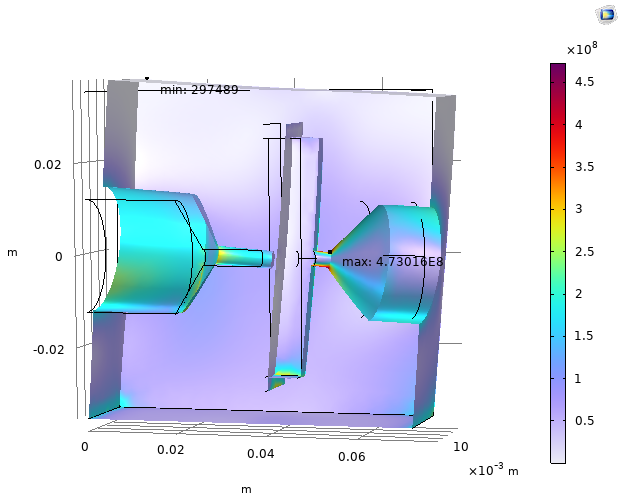
\includegraphics[width=.6\textwidth]{ Static_FEA_StressMagnitude1.png}
                \caption{Static FEA Results on simplified Single Body Model}
                \label{fig:FEAdisp}
            \end{figure}




	
\textbf{Actuator-Housing Weldment}
\begin{enumerate}[label=\roman*.]

	\item In addition to stresses applied by the internal pressure, there is also stress on the 
		actuator mount and its' radial weld due to thermal expansion and contraction. This was
		identified as a potential failure mode for this weld specifically as the other welds 
		are invar-invar and have predictable mechanical properties and a relatively low expansion
		rate constant across all members in the weldment.
  \item \textbf{Purpose.}
    The purpose of this analysis is to verify that welding is a viable method for joining 
		the actuator subsystem to the housing. Thermal contraction of the actuator mount combined 
		with potential weld embrittlement could cause failure. Further analysis is needed to inform
		weld reliability or alternate suggestions 
  \item \textbf{Assumptions, Principles, and Methods.}
    The weld joints are treated as full penetration fillet welds, and the same assumptions made 
		for the housing weld analysis hold for the material properties and radiographic inspection 
		of the actuator mount to housing weld.
  \item \textbf{Calculations.}
 		The mount being made of Allvar has an anisotropic quality. It has a positive axial coefficient
  	of thermal expansion that is 2 $\mu$m/m greater than the magnitude of the negative axial 
  	expansion amounting to 32 $\mu$m/m. The greatest change in radius $\Delta R$ occurs across the cold side of the 
  	temperature gradient with
		$\Delta R = R_0 \left(1 - \left(-\alpha_{\text{alv}}\right)\right) \Delta T_{\text{cold}}=0.0254mm$
		This is a basic confined thermal expansion problem and the maximum stress on the Allvar and 
		the weld due to the thermal expansion can be  calculated by finding the stress necessary to
		deform the Allvar mount by that amount:
		\begin{equation}
			\sigma_{\text{alv}} = \frac{E_{\text{allvar}} \cdot \Delta R}{R_0} = \frac{55\times10^{9} \cdot 0.0254 \text{ mm}}{18 \text{ mm}} = 74.86 \text{ MPa}
		\end{equation}
  \item \textbf{Results.}
		The area of the weld and the area of the mount in contact with it are the same, and thus the
 		stresses are the same. Given that this stress is much smaller than the yield stress of Allvar 
 		and of the weld metal we find a sufficient safety factor:
		$$\text{FS} = \frac{S_{y,\text{weld}}}{\sigma_{\text{weld}}=3.68}$$
  \item \textbf{Discussion.}
		While this FS is acceptable, this is assuming the weld has the same material properties as
 		the invar housing. In reality, the material mismatch in the mount-housing weld may lead to 
 		detrimental changes in material properties around the weld area which could cause a variety
  	of failures. Because Allvar 30 is a experimental alloy with a proprietary composition we 
  	cannot verify the feasibility of this weld. Representatives from the Allvar team advised against 
  	welding Allvar to invar or other iron alloys as the titanium from the Allvar will combine with
   	the iron to create brittle intermetallic compounds making the weld brittle. 
		Methods to counter this include using a ductile interface layer that can aid in mitigating 
		creation of brittle compounds, but this could be highly involved and experimental. A recommended
 		path would be to use fasteners with a slight mount redesign that allows for bolting into the
  	housing. This would require some additional research into sealing but is the simplest and most 
  	reliable solution.
\end{enumerate}

\textbf{Housing Outlet Wall}
\begin{enumerate}[label=\roman*.]
	\item \textbf{Purpose.}
	The purpose of this analysis is to verify that the housing outlet wall maintains structural integrity under the pressure exerted on it 
	by the internal gas flow. This wall could be a problem due to how thin it is and how much pressure will be exerted on it. Using the pressure
	hand calculations, the Factor of Safety (FS) can be calculated to determine if the wall is thick enough to withstand the pressure exerted on it.

	\item \textbf{Assumptions, Principles, and Methods.}
	The wall is treated as a circular plate with fixed edges under uniform distributed pressure of \specPressure. The maximum stress is calculated using the formula for
	a flat plate with fixed edges under uniform distributed loading. The parameters used in this analysis are diameter of the plate is 3.5 mm and the thickness is 1 mm.
	\item \textbf{Calculations.}
	The total force acting on the outlet wall is first found from the applied pressure and plate area:
	 \begin{equation}
        F = P \cdot A = P \cdot \pi r^2
        = (68.95 \times 10^6~\text{Pa})\,(\pi)(0.00175~\text{m})^2
        = 663~\text{N}
    \end{equation}
	The maximum bending stress in a circular plate with fixed edges under uniform pressure (occurring at the outer edge) is given by:
	    \begin{equation}
        \sigma_{\max} = \frac{3\,P\,r^2\,}{4\,t^2}
    \end{equation}
    Substituting values:
    \begin{equation}
        \sigma_{\max}
        = \frac{3\,(68.95 \times 10^6)\,(0.00175)^2\,}
               {4\,(0.001)^2}
        = 158.4~\text{MPa}
    \end{equation}
	where P is the pressure, r is the radius of the plate, and t is the thickness of the plate.

	\item \textbf{Results.}
	    \begin{equation}
        \text{FS} = \frac{S_{y,\,\text{Invar}}}{\sigma_{\max}}
                   = \frac{240~\text{MPa}}{158.4~\text{MPa}}
                   = 1.51
    \end{equation}

	\item \textbf{Discussion.}
	Because the factor of safety for the housing outlet wall is greater than 1, the wall will not fail under the pressure exerted on it. The wall may deform slightly, but it 
	is not enough to significantly affect the effctive diameter or anything else that would cause the device to fail. This shows that this failure mode will
	not a be major concern for the design and the wall is thick enough so that the pressure will not cause it to fail. 

\end{enumerate}

\textbf{Orifice Channel Opening}
\begin{enumerate}[label=\roman*.]
	\item \textbf{Purpose.}
	The purpose of this analysis is to verify that the orifice channel opening maintains structural integrity under the pressure exerted on it by the internal 
	gas flow. The opening creates a stress concentration at the corner where the fluid flow exits the orifice. Using Finite Element Analysis (FEA) testing to see
	the stress exerted on that corner, the Factor of Safety (FS) can then be calculated using the yield strength of Invar.
	\item \textbf{Assumptions, Principles, and Methods.}
	The assumpptions for the Orifice Channel Opening are using the FEA results to find the maximum and average von Mises stress at the corner of the outlet opening.
	Reference the following chapter, Testing, for the complete priciples and metthods used for testing and FEA.
	\item \textbf{Calculations.}
	Using the data from the FEA testing, the factor of safety at the corner can be found. 

	See \ref{fig:FEAdisp2} in Apendix Afor data from the FEA testing that will be used to calculate the FS at the corner of the outlet opening.

	


	The maximum von Mises stress at the corner of the outlet opening is 300 MPa and the average von Mises stress is 178 MPa. Using the yield strength of annealed Invar (240 MPA), 
	the FS can be calculated for both the maximum and average stress values.
	\item \textbf{Results.}
	
	Using the maximum von Mises stress:
	$FS = \frac{240 \text{MPa}}{300 \text{MPa}} = 0.8$

	Using the average von Mises stress:
	$FS = \frac{240 \text{MPa}}{178 \text{MPa}} = 1.35$

	The FS less than 1 at the maximum stress is an issue and something that needs to be addressed, however because the average stress is greater than 1, it is likely that the corner will not fail under most operating conditions.
	\item \textbf{Discussion.}
	The FS calculated using the maximum von Mises stress is less than 1, which indicates that the corner of the outlet opening could fail if the pressure is at its maximum. However, 
	the FS at average von Mises stress is greater than 1, which indicates that at most operating conditions, this corner will not be a problem. In order to make the corner more robust, 
	the corner could be rounded to reduce the stress concentration. This would increase the FS because it would lower the stress that is put on that point. Another way to increase the FS
	would be to increase the thickness of the wall at that point, which would also lower the stress. Ultimately, rounding the corner is probably the best solution because it is a simple and 
	easy way to reduce the stress concentration without adding more material. 
\end{enumerate}

	\section{Tolerance Failure Analysis}
	\label{subsec:DFMEA::tol}

		The final failure mode --- namely, failure to meet the Required Relationship in equation~\eqref{eq:required_relationship} --- encapsulates several sources off error that affect the input-output relationship of the \device.
		Nominal satisfaction of the Required Relationship was demonstrated in Section~\ref{sec:design:just}, but system precision must be evaluated holistically and numerically.

		\textbf{System Output Fidelity}
		\begin{enumerate}[label=\roman*.]
			\item \textbf{Purpose.}
				To quantitatively evaluate the effect of various errors on the system performance, the open-loop passive system transfer function in Figure~\ref{fig:TF_RR} must be revised to account for the impact of these errors.
				This provides a comprehensive estimation of the system's ability to meet the Required Relationship for all temperatures.
			\item \textbf{Assumptions, Principles, and Methods.}
				The Transfer Function analysis accounts for four sources of error: heat transfer from the hot internal gas, dimensional errors, variations in the actuator's thermal expansion, thermal expansion of the valve subcomponents, the spring reaction force of the bellows, and the orifice fillet radius produced by the wire EDM cut.
				Other unquantifiable errors will be present that cannot be properly quantified; these will be addressed in Chapter~\ref{chap:concl}.
			\item \textbf{Calculations.}
				Derivation and calculation of the full System Output Transfer Function is presented in Appendix~\ref{app:sat}. The derived values were encoded with a script to enable efficient parameter variation.
				The function evaluates heat transfer, varies the machined length of all critical dimensions according to a normalized tolerance distribution, computes the thermal expansion of each part,
				resolves the resulting spring force balance driven by the bellows, sums the resulting part lengths to obtain the position of each orifice square, and converts their difference to the final output diameter. 
			\item \textbf{Results.}
				The results are plotted and interpreted in detail in Appendix~\ref{app:sat:TF:results}. To account for variable sources of error, the Transfer Function takes a large number of samples and
				produces a normalized distribution. It estimates that 90.6\% of all devices machined will produce an output within tolerance for all temperatures.
				It calculates the effect of calibration, which will only be needed for the remaining 9.4\%, and confirms that these will also meet their requirement if the calibration precision
				specified in Appendix~\ref{app:calcs:cal:sat} (a \SI{14.3}{\degree} rotation of the calibration screw) are met or exceeded.
			\item \textbf{Discussion.}
				The \device, despite several significant sources of error, meets and exceeds a strict passive output requirement across a wide temperature range. This estimation is optimistic and cannot account for
				some sources of error, such as binding friction, weld precision, and the effect of the calibration stack on thermal expansion. As laid out in Chapter~\ref{chap:concl}, these should be more carefully
				evaluated as the design is further iterated.
		\end{enumerate}
 
\chapter{Testing}
\label{chap:test}

	\section{Objective}
	In the absence of a physical manufactured model, verification of the DFMEA is
	done through two methods: (1) Analytical methods and (2) Finite element
	simulations. This section discusses the testing process and strategy of using
	finite element simulations to validate the analytical results and explore
	failure modes determined by DFMEA. This computational prototype will be
	subjected to the following simulations: Heat Transfer (HT), Computational Fluid
	Dynamics (CFD), and Multibody Dynamics (MBD).

	\section{Test Design}
	To make the simulations computationally less expensive, the following
	strategies have been employed
	\begin{enumerate}
			\item The PTCD is cut in half about its vertical symmetry plane, creating
			new surfaces which will be referred to as ``symmetry surfaces'' shown in \ref{fig:symmetryplane}. By setting
			the exposed symmetry surfaces to its appropriate ``symmetrical nodes'' in
			the simulation software, the amount of meshes can be cut in half, reducing
			the computation time. 
			\begin{figure}[H]
									\centering
									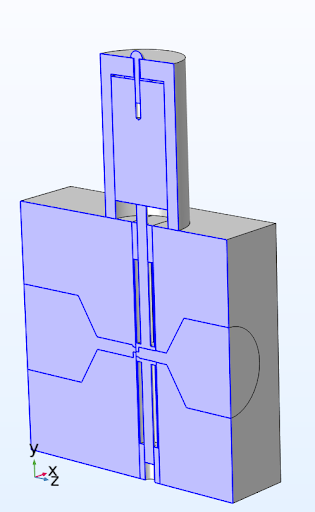
\includegraphics[width=.25\textwidth]{figures3/testingch_symmetry.png}
									\caption{This figure highlights the symmetry plane}
									\label{fig:symmetryplane}
			\end{figure}
			\item The physics is ``decoupled''. The CFD is run on a rigid negative
			domain (seen in \ref{fig:fluidvolume})of the channel with a turbulent simulation where a ``pressure map''
			of the wetted surface is recovered. This same pressure map is used to apply
			a load on the wetted surfaces of the PTCD assembly geometry to apply a load
			that is representative of the fluid flow during operation. The heat transfer
			simulation is then executed on the loaded assembly by setting all exposed
			surfaces to the ambient temperature, and all the wetted surfaces to the
			fluid temperature.
			\begin{figure}[H]
									\centering
									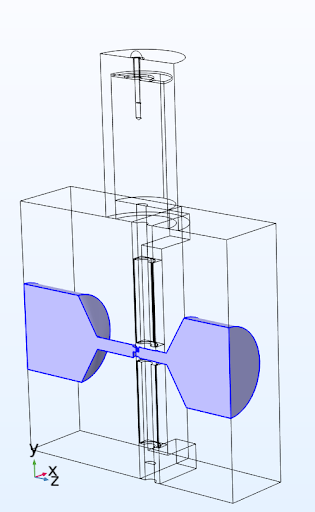
\includegraphics[width=.25\textwidth]{figures3/testingch_negative.png}
									\caption{This domain represents the fluid, it conforms to the volume of the cavity}
									\label{fig:fluidvolume}
			\end{figure}
			\item As additional verification, a solid mechanics simulation was conducted
			on single bodies like the orifice and the inlet/outlet parts, isolated from
			the assembly. This form of isolated simulation was also conducted for HT.
			\item A physics driven mesh is selected as a blanket parameter for the
			entire assembly with an effective diameter smaller than the radius of the
			smallest fillet in our geometry. On top of the blanket parameter, specific
			parts in the assembly have modified mesh parameters; Namely the orifice,
			mount, and the actuator have twice the mesh resolution.
	\end{enumerate}

	\section{Developing the computational prototype}

	\subsection{Fluid Dynamics Simulation}
	Fluid dynamics simulation is conducted to recover a pressure map on the
	fluid-solid interface. This pressure map will be used as the boundary load for
	the multi-body simulation.

	\subsubsection{Boundary Condition Decisions}
	\begin{enumerate}
			\item The inlet and outlet are assumed to be in fully developed flow
			\begin{enumerate}
					\item Inlet pressure is swept across the design space with parameters
					from $10^{2}$ psi to $10^{4}$ psi in increments of $10^{0.5}$ psi. This
					decision to have an exponential sweep was made because of the range
					\item Outlet pressure is set as 0 psi
			\end{enumerate}
			\item The boundary condition is set as no slip.
	\end{enumerate}

	\subsubsection{Data Collection}
	The pressure map on the fluid-solid interface is recovered and mapped onto the
	wetted surface of the multi-body simulation. The pressure map is shown to be created by the fluid dynamics as shown in \ref{fig:pressuremap}.
	\begin{figure}[H]
									\centering
									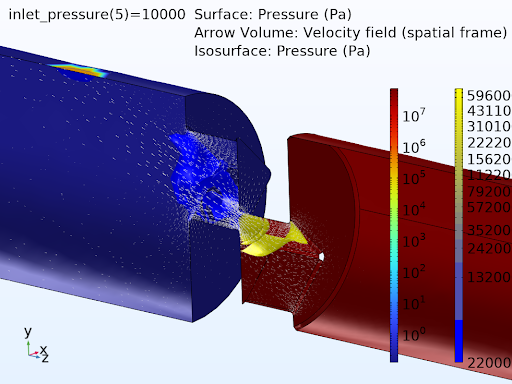
\includegraphics[width=.75\textwidth]{figures3/testingch_pressuremap.png}
									\caption{A close up of the orifice showing a massive pressure drop with isobaric surfaces}
									\label{fig:pressuremap}
	\end{figure}
	\subsubsection{Limitations}
	The computational model used is k-epsilon with the fluid set as incompressible.
	This is a very simplistic model that does not accurately compute the state of
	the fluid in the volume.

	\subsection{Heat Transfer Simulation}
	To validate the analytical calculations on the PTCD's dimensional stability
	under operating temperature conditions, a heat transfer simulation is conducted
	by a steady state(fig \ref{fig:tempgrad}) and transient study.
	\begin{figure}[H]
									\centering
									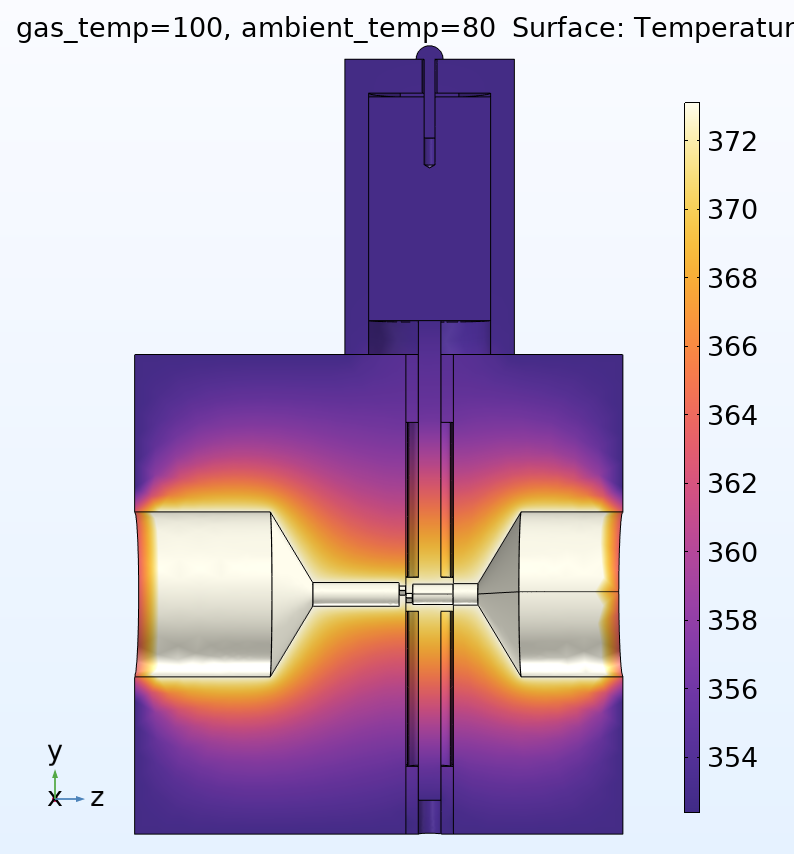
\includegraphics[width=.45\textwidth]{figures3/testingch_tempgrad.png}
									\caption{temperature gradient at the maximum temperature setting of the design space.}
									\label{fig:tempgrad}
	\end{figure}

	\subsubsection{Boundary Condition Decisions}
	The isolated heat transfer tests used two different boundary-condition setups.
	Each study type still shared common mechanical constraints. However, the
	distinctions in boundary-conditions enabled the different end results of each
	respective study.

	For the steady state heat transfer test there the operating temperature range
	was parametrically swept to the environmental temperatures. Since the sweep
	evaluates only equilibrium states, the path of how heat reaches the body is
	irrelevant. The final uniform temperature is physically correct for the steady
	state and numerically efficient across the entire boundary. This boundary
	condition produced the stroke versus temperature data that was validated
	against the analytical model.

	The time-dependent study required different thermal boundary conditions. Since
	a prescribed surface temperature forced the exterior to jump quasi-statically,
	there was no need for the temperature boundary condition to be considered as it
	was in the steady state heat transfer test. Instead, there was a heat flux
	condition on the exterior boundaries characterized by a convective coefficient
	$h$ and an external ambient temperature $T_{ext}$. The ambient temperature was
	driven by the following step function:
	\[
			T_{ext}(t) = T_{ref} + \SI{20}{\kelvin}\times \mathrm{tstep}(t),
	\]
	The initial condition sets the entire assembly to $T_{ref}$ which is in
	equilibrium with the original ambient temperature. This setup reproduces the
	physical scenario where the body convects toward a stepped ambient temperature
	and yields a first-order thermal response used to extract the time constant.

	\subsubsection{Data Collection}
	The steady-state heat transfer data were gathered by sweeping $T_{env}$ across
	the operating range and recording the converged actuator stroke at each point.
	The primary output was the axial displacement of the orifice evaluated as a
	point quantity and taken as the device stroke. Each solve returns a single
	equilibrium displacement, and the collection of these points forms the
	stroke-versus-temperature curve compared against the analytical prediction in
	the Results section. The sweep was run in \SI{5}{\kelvin} increments with
	convergence behavior across the entire temperature range.

	The time dependent heat transfer test data was gathered from a single
	time-dependent solve for the \SI{20}{\kelvin} ambient step. the point
	temperature and corresponding displacement at fixed output intervals over a
	two-hour simulated window (\texttt{range(0, 60, 7200)}). This window was chosen
	to extend well past the expected settling time so the full approach to the new
	equilibrium was captured.

	\subsubsection{Limitations}
	The primary limitation for both heat transfer tests was the model. The model
	used was a reduced-order representation of the device's core instead of the
	entire PTCD assembly. This model included the actuator, the house, cylindrical
	equivalents for the bellows, and the center housing pieces. While smaller
	components such as the fasteners were included, the outer housing and bellows
	geometry were omitted. This was a deliberate simplification that enabled the
	stationary sweep to converge cleanly across the entire temperature range and
	for the transient study to resolve to a first-order time constant response.
	However, this simplification characterizes the orifice, actuator, and mount
	expansion mechanism in isolation rather than the entire device. The retained
	components capture the actual path that set the stroke which is why the results
	of the steady state study agree with the analytical model within
	\SI{0.2}{\percent}. This simplification, while a limitation, also preserves the
	physics that matter most for the actuation of the PTCD.

	Other limitations include the replacement of the bellows. Their cylindrical
	equivalent reproduces the correct axial spring stiffness but not the detailed
	geometry, thermal behavior, or local stiffening of the actual part. Thermal
	contact resistance at the bonded interfaces were also omitted. This assumes the
	boundaries of each mate have perfectly conducting and slow heat propagation.
	This potentially lengthens the acclimation time making the reported time
	constant smaller than that of the entire assembly.

	By and large the simplifications in the model best are valid characterizations
	of the differential-expansion stroke mechanism and its approximate transient
	behavior.

	\subsection{Multi-body Simulation}
	To gain a beginning intuition on the PTCD housing's reaction to applied pressure
	and inform higher fidelity models a simplified single body model was made. The
	single body model joins the housing components as a single solid avoiding use of
	complicated mates and relations. While this assumption does reduce accuracy to
	real performance, it allows for quick computation and as an initial method it
	avoids errors and non-convergence that can come from more complex models. The
	max pressure of \specPressure\ was applied to all wetted surfaces. This provides
	a general worst case stress result as in reality pressure will vary with fluid
	flow dynamics. Results were compared with hand calculations for simpler parts of
	the housing and verified that the simulation delivers expected results, and can
	be expected to do so for non-trivial surfaces. The results of this test are
	utilized in the DFMEA .

	To validate the analytical calculations on the PTCD's dimensional stability
	under load from the fluid pressure, a multi-body simulation is conducted by
	using the pressure map recovered from the fluid dynamics simulation and setting
	it as a boundary load in the wetted surface.
	The multi-body simulation takes into account the interaction between the
	components of the PTCD with appropriate surface relationships. Welded surfaces
	are set as identity pairs that keep the surface meshes together while other
	surfaces which are
	 expected to collide are set as Contact pairs to simulate
	collision.
\chapter{Testing}
\label{chap:test}

\section{Objective}
In the absence of a physical manufactured model, verification of the DFMEA is
done through two methods: (1) Analytical methods and (2) Finite element
simulations. This section discusses the testing process and strategy of using
finite element simulations to validate the analytical results and explore
failure modes determined by DFMEA. This computational prototype will be
subjected to the following simulations: Heat Transfer (HT), Computational Fluid
Dynamics (CFD), and Multibody Dynamics (MBD).

\section{Test Design}
To make the simulations computationally less expensive, the following
strategies have been employed
\begin{enumerate}
    \item The PTCD is cut in half about its vertical symmetry plane, creating
    new surfaces which will be referred to as ``symmetry surfaces'' shown in \ref{fig:symmetryplane}. By setting
    the exposed symmetry surfaces to its appropriate ``symmetrical nodes'' in
    the simulation software, the amount of meshes can be cut in half, reducing
    the computation time. 
    \begin{figure}[H]
                \centering
                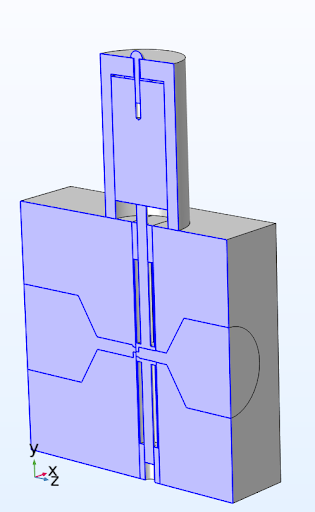
\includegraphics[width=.25\textwidth]{figures3/testingch_symmetry.png}
                \caption{This figure highlights the symmetry plane}
                \label{fig:symmetryplane}
    \end{figure}
    \item The physics is ``decoupled''. The CFD is run on a rigid negative
    domain (seen in \ref{fig:fluidvolume})of the channel with a turbulent simulation where a ``pressure map''
    of the wetted surface is recovered. This same pressure map is used to apply
    a load on the wetted surfaces of the PTCD assembly geometry to apply a load
    that is representative of the fluid flow during operation. The heat transfer
    simulation is then executed on the loaded assembly by setting all exposed
    surfaces to the ambient temperature, and all the wetted surfaces to the
    fluid temperature.
    \begin{figure}[H]
                \centering
                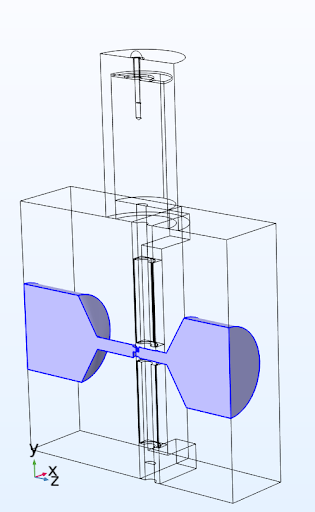
\includegraphics[width=.25\textwidth]{figures3/testingch_negative.png}
                \caption{This domain represents the fluid, it conforms to the volume of the cavity}
                \label{fig:fluidvolume}
    \end{figure}
    \item As additional verification, a solid mechanics simulation was conducted
    on single bodies like the orifice and the inlet/outlet parts, isolated from
    the assembly. This form of isolated simulation was also conducted for HT.
    \item A physics driven mesh is selected as a blanket parameter for the
    entire assembly with an effective diameter smaller than the radius of the
    smallest fillet in our geometry. On top of the blanket parameter, specific
    parts in the assembly have modified mesh parameters; Namely the orifice,
    mount, and the actuator have twice the mesh resolution.
\end{enumerate}

\section{Developing the computational prototype}

\subsection{Fluid Dynamics Simulation}
Fluid dynamics simulation is conducted to recover a pressure map on the
fluid-solid interface. This pressure map will be used as the boundary load for
the multi-body simulation.

\subsubsection{Boundary Condition Decisions}
\begin{enumerate}
    \item The inlet and outlet are assumed to be in fully developed flow
    \begin{enumerate}
        \item Inlet pressure is swept across the design space with parameters
        from $10^{2}$ psi to $10^{4}$ psi in increments of $10^{0.5}$ psi. This
        decision to have an exponential sweep was made because of the range
        \item Outlet pressure is set as 0 psi
    \end{enumerate}
    \item The boundary condition is set as no slip.
\end{enumerate}

\subsubsection{Data Collection}
The pressure map on the fluid-solid interface is recovered and mapped onto the
wetted surface of the multi-body simulation. The pressure map is shown to be created by the fluid dynamics as shown in \ref{fig:pressuremap}.
\begin{figure}[H]
                \centering
                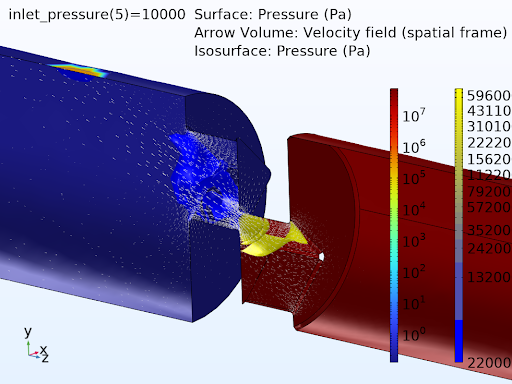
\includegraphics[width=.75\textwidth]{figures3/testingch_pressuremap.png}
                \caption{A close up of the orifice showing a massive pressure drop with isobaric surfaces}
                \label{fig:pressuremap}
\end{figure}
\subsubsection{Limitations}
The computational model used is k-epsilon with the fluid set as incompressible.
This is a very simplistic model that does not accurately compute the state of
the fluid in the volume.

\subsection{Heat Transfer Simulation}
To validate the analytical calculations on the PTCD's dimensional stability
under operating temperature conditions, a heat transfer simulation is conducted
by a steady state(fig \ref{fig:tempgrad}) and transient study.
\begin{figure}[H]
                \centering
                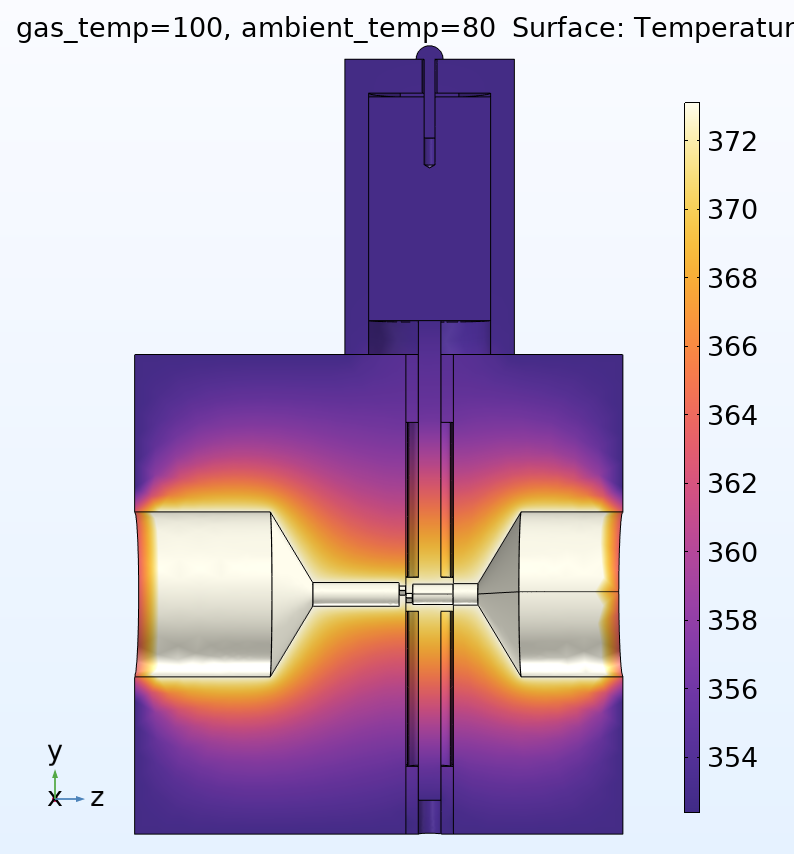
\includegraphics[width=.45\textwidth]{figures3/testingch_tempgrad.png}
                \caption{temperature gradient at the maximum temperature setting of the design space.}
                \label{fig:tempgrad}
\end{figure}

\subsubsection{Boundary Condition Decisions}
The isolated heat transfer tests used two different boundary-condition setups.
Each study type still shared common mechanical constraints. However, the
distinctions in boundary-conditions enabled the different end results of each
respective study.

For the steady state heat transfer test there the operating temperature range
was parametrically swept to the environmental temperatures. Since the sweep
evaluates only equilibrium states, the path of how heat reaches the body is
irrelevant. The final uniform temperature is physically correct for the steady
state and numerically efficient across the entire boundary. This boundary
condition produced the stroke versus temperature data that was validated
against the analytical model.

The time-dependent study required different thermal boundary conditions. Since
a prescribed surface temperature forced the exterior to jump quasi-statically,
there was no need for the temperature boundary condition to be considered as it
was in the steady state heat transfer test. Instead, there was a heat flux
condition on the exterior boundaries characterized by a convective coefficient
$h$ and an external ambient temperature $T_{ext}$. The ambient temperature was
driven by the following step function:
\[
    T_{ext}(t) = T_{ref} + \SI{20}{\kelvin}\times \mathrm{tstep}(t),
\]
The initial condition sets the entire assembly to $T_{ref}$ which is in
equilibrium with the original ambient temperature. This setup reproduces the
physical scenario where the body convects toward a stepped ambient temperature
and yields a first-order thermal response used to extract the time constant.

\subsubsection{Data Collection}
The steady-state heat transfer data were gathered by sweeping $T_{env}$ across
the operating range and recording the converged actuator stroke at each point.
The primary output was the axial displacement of the orifice evaluated as a
point quantity and taken as the device stroke. Each solve returns a single
equilibrium displacement, and the collection of these points forms the
stroke-versus-temperature curve compared against the analytical prediction in
the Results section. The sweep was run in \SI{5}{\kelvin} increments with
convergence behavior across the entire temperature range.

The time dependent heat transfer test data was gathered from a single
time-dependent solve for the \SI{20}{\kelvin} ambient step. the point
temperature and corresponding displacement at fixed output intervals over a
two-hour simulated window (\texttt{range(0, 60, 7200)}). This window was chosen
to extend well past the expected settling time so the full approach to the new
equilibrium was captured.

\subsubsection{Limitations}
The primary limitation for both heat transfer tests was the model. The model
used was a reduced-order representation of the device's core instead of the
entire PTCD assembly. This model included the actuator, the house, cylindrical
equivalents for the bellows, and the center housing pieces. While smaller
components such as the fasteners were included, the outer housing and bellows
geometry were omitted. This was a deliberate simplification that enabled the
stationary sweep to converge cleanly across the entire temperature range and
for the transient study to resolve to a first-order time constant response.
However, this simplification characterizes the orifice, actuator, and mount
expansion mechanism in isolation rather than the entire device. The retained
components capture the actual path that set the stroke which is why the results
of the steady state study agree with the analytical model within
\SI{0.2}{\percent}. This simplification, while a limitation, also preserves the
physics that matter most for the actuation of the PTCD.

Other limitations include the replacement of the bellows. Their cylindrical
equivalent reproduces the correct axial spring stiffness but not the detailed
geometry, thermal behavior, or local stiffening of the actual part. Thermal
contact resistance at the bonded interfaces were also omitted. This assumes the
boundaries of each mate have perfectly conducting and slow heat propagation.
This potentially lengthens the acclimation time making the reported time
constant smaller than that of the entire assembly.

By and large the simplifications in the model best are valid characterizations
of the differential-expansion stroke mechanism and its approximate transient
behavior.

\subsection{Multi-body Simulation}
To gain a beginning intuition on the PTCD housing's reaction to applied pressure
and inform higher fidelity models a simplified single body model was made. The
single body model joins the housing components as a single solid avoiding use of
complicated mates and relations. While this assumption does reduce accuracy to
real performance, it allows for quick computation and as an initial method it
avoids errors and non-convergence that can come from more complex models. The
max pressure of \specPressure\ was applied to all wetted surfaces. This provides
a general worst case stress result as in reality pressure will vary with fluid
flow dynamics. Results were compared with hand calculations for simpler parts of
the housing and verified that the simulation delivers expected results, and can
be expected to do so for non-trivial surfaces. The results of this test are
utilized in the DFMEA .

To validate the analytical calculations on the PTCD's dimensional stability
under load from the fluid pressure, a multi-body simulation is conducted by
using the pressure map recovered from the fluid dynamics simulation and setting
it as a boundary load in the wetted surface.
The multi-body simulation takes into account the interaction between the
components of the PTCD with appropriate surface relationships. Welded surfaces
are set as identity pairs that keep the surface meshes together while other
surfaces which are expected to collide are set as Contact pairs to simulate
collision.

\subsubsection{Boundary Condition Decisions}
\begin{enumerate}
    \item Surface pairs and contact constraints.
    \begin{enumerate}
        \item In multi-body simulation, the consideration for surface pairs
        where the multiple bodies contact is pivotal for accuracy of results.
        For all simulations, the welded surfaces are set as \textbf{identity
        pair} while surfaces that are unwelded and expected to collide are set
        as \textbf{contact pairs} as shown in fig \ref{fig:both_label}.
\begin{figure}[H]
    \centering
    \begin{subfigure}[t]{0.45\textwidth}
        \centering
        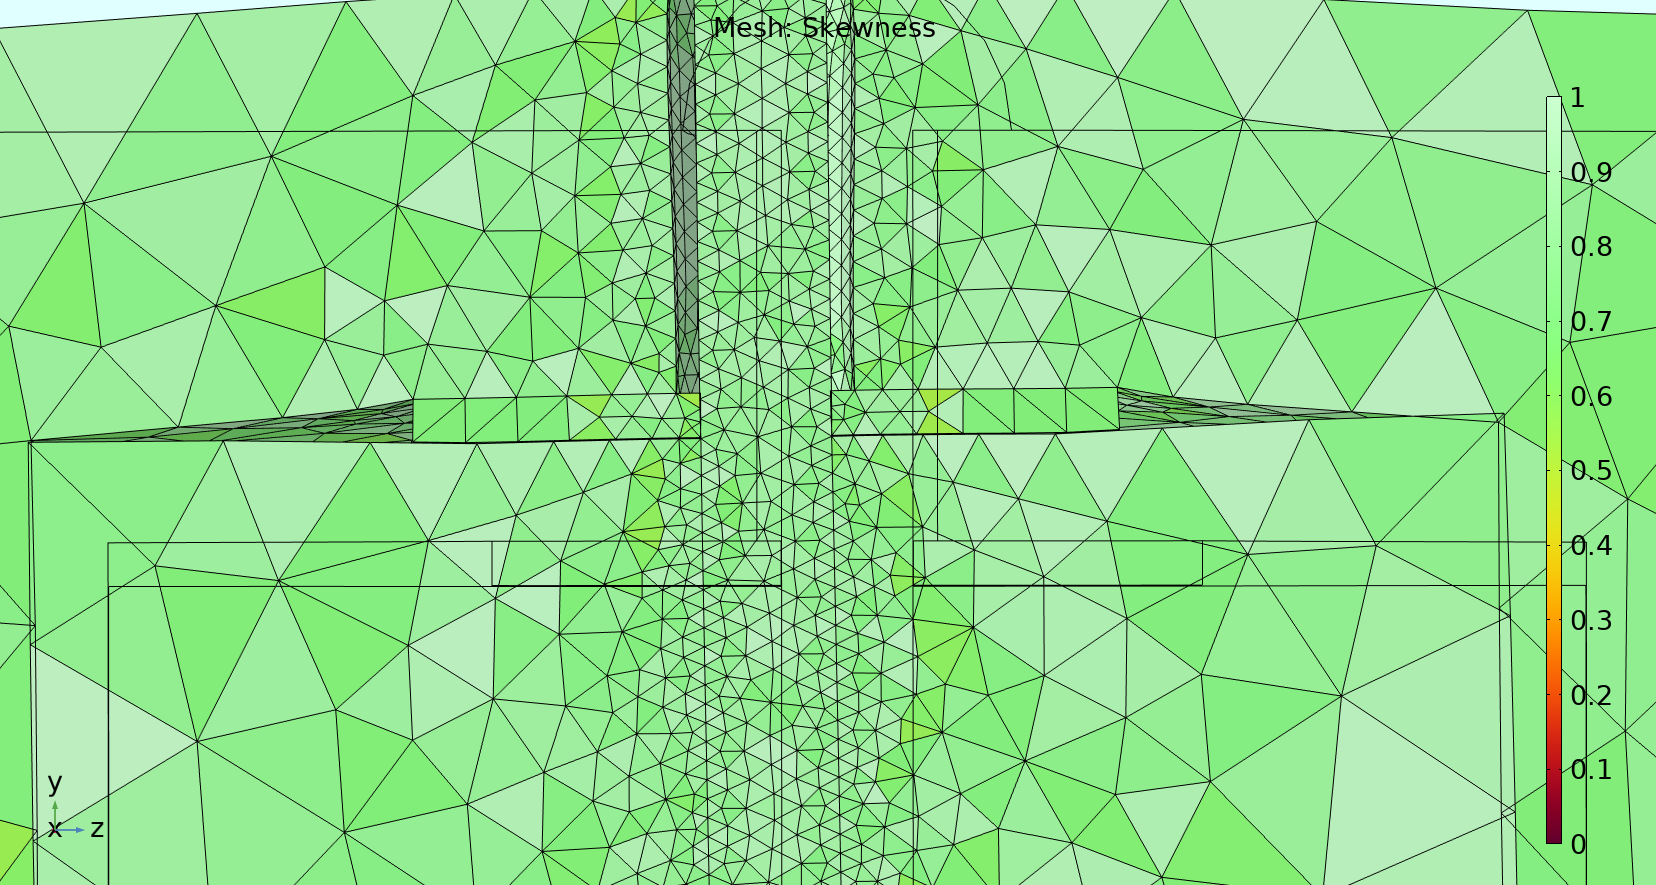
\includegraphics[width=\textwidth]{figures3/testingch_contact_pair.png}
        \caption{Demonstration of how surfaces set as contact pair react.}
        \label{fig:contactpair}
    \end{subfigure}
    \begin{subfigure}[t]{0.45\textwidth}
        \centering
        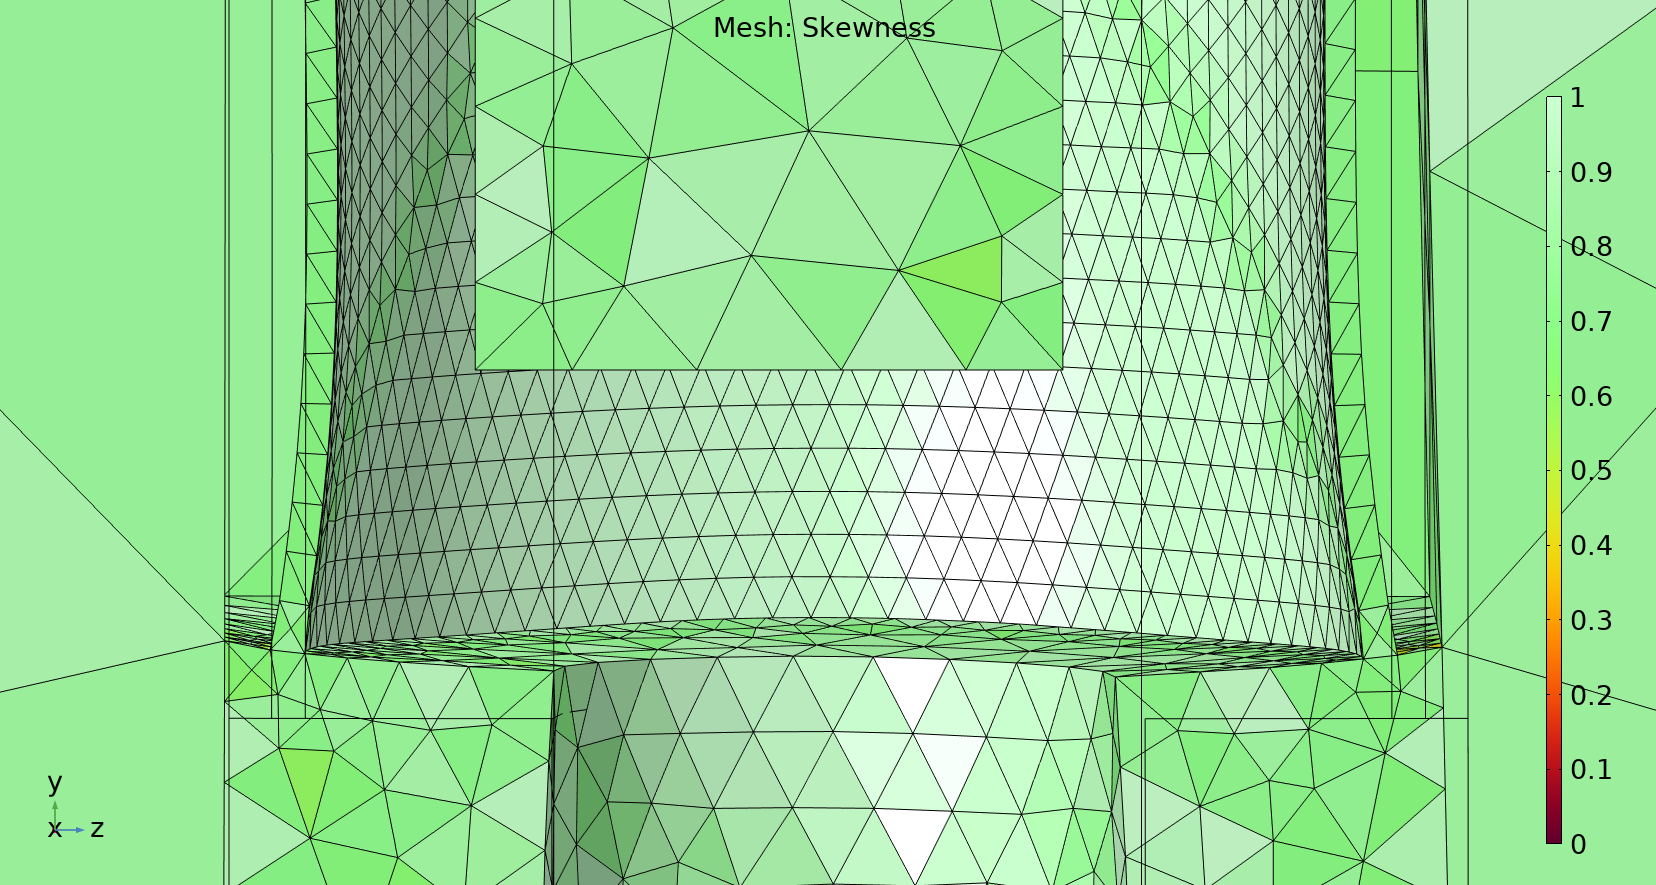
\includegraphics[width=\textwidth]{figures3/testingch_identity_pair.png}
        \caption{Demonstrationn of how identity pairs simulate a weld.}
        \label{fig:identitypair}
    \end{subfigure}
    \caption{Surface pair comparison}
    \label{fig:both_label}
\end{figure}
        % [PHOTO] Contact mesh (mesh skewness) at the orifice / housing interface.
        \item Failure to set up these surface constraints will result in bodies
        phasing through each other, welded surfaces to decouple, and so on.
        \item Verification for the correctness of contact constraints are made
        by setting a rigid translation of the orifice in space and observing how
        the meshes behave. This is shown on fig \ref{fig:displacement} below.
		\begin{figure}[H]
                \centering
                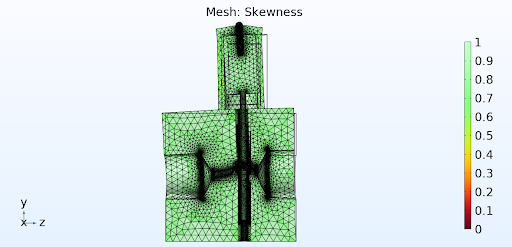
\includegraphics[width=.90\textwidth]{figures3/AbrAkAdAbrA_teST.png}
                \caption{temperature gradient at the maximum temperature setting of the design space.}
                \label{fig:displacement}
\end{figure}
    \end{enumerate}
    \item Fluid-solid boundaries (incorporating union nodes where a single
    continuous boundary is required for FSI).
    \item Accurate boundary representations for complex orifice shapes, ensuring
    internal flow geometries are not oversimplified as standard cylinders.
\end{enumerate}

\subsubsection{Data Collection}
Surface data will be collected on weld joints and failure points identified by
DFMEA. These data can be recovered at any point in the PTCD as shown in fig \ref{fig:stressnstrain}.
\begin{figure}[H]
    \centering
    \begin{subfigure}[t]{0.45\textwidth}
        \centering
        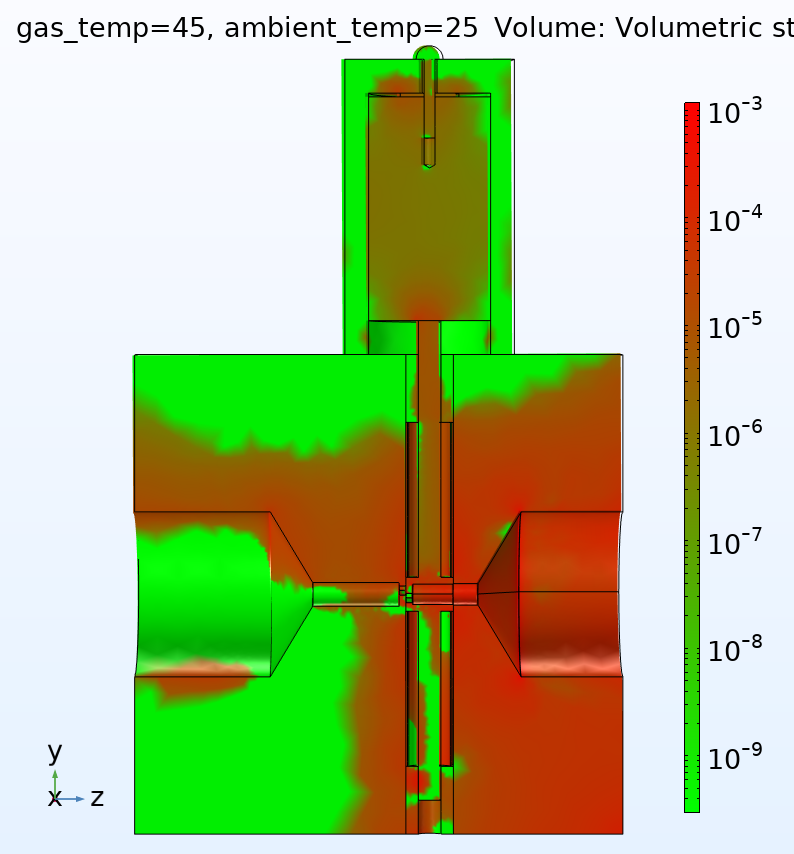
\includegraphics[width=\textwidth]{figures3/testing_ch_volstrain.png}
        \caption{Volumetric strain}
        \label{fig:straindata}
    \end{subfigure}
    \begin{subfigure}[t]{0.45\textwidth}
        \centering
        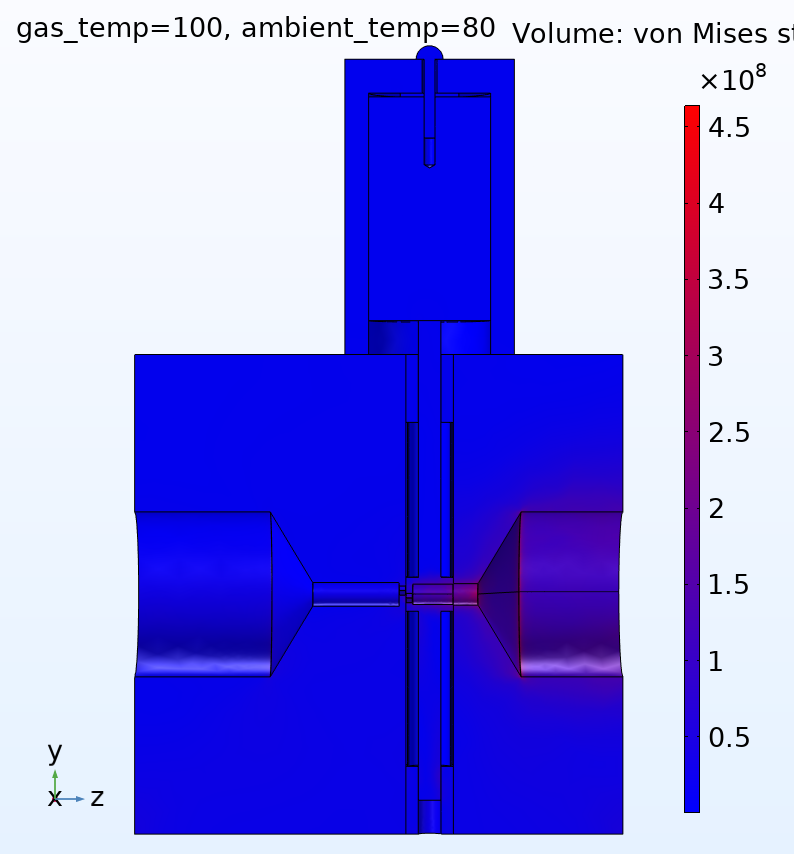
\includegraphics[width=\textwidth]{figures3/testing_ch_volstress.png}
        \caption{Von-Misses Stress}
        \label{fig:stressdata}
    \end{subfigure}
    \caption{Stress and strain map}
    \label{fig:stressnstrain}
\end{figure}
\subsubsection{Limitations}
Several simplifications were introduced to the multi-body simulation to prioritize numerical convergence and reduce overall geometric complexity. 
Contact friction between interacting surfaces was omitted from the model entirely. 
To bypass the heavy computational cost of meshing, the Inconel bellows were represented using an equivalent material model rather than their true physical geometry. 
Similarly, the screw and washer were modeled as a continuous union rather than discrete interactive components. The Allvar component was approximated with an isotropic coefficient of thermal expansion based on nominal textbook values, which inherently neglects the alloy's true anisotropic thermal behavior.


\section{Results}


\subsection{Other relevant results/Discussion}

\subsubsection{Heat Transfer}
The stationary parametric sweep converged across the full \SI{-60}{\celsius} to
\SI{80}{\celsius} operating range and reproduced the analytical stroke model.
The two FEA anchor points at $\Delta T = \SI{5}{\kelvin}$ and
$\Delta T = \SI{10}{\kelvin}$ returned actuator displacements of
\SI{5.58}{\micro\meter} and \SI{11.14}{\micro\meter}, establishing a slope of
\SI{1.115}{\micro\meter\per\kelvin} and matching the analytical prediction
within \SI{0.2}{\percent}.

The time-dependent study, run for a representative \SI{20}{\kelvin} ambient
step, produced a clean first-order exponential response at the monitored
actuator point, rising from \SI{25}{\celsius} toward a steady-state plateau of
approximately \SI{44.8}{\celsius} (Figure~\ref{fig:transient}). The thermal time
constant was $\tau \approx \SI{500}{\second}$ (about \SI{8}{\minute}), read as
the time to reach \SI{63}{\percent} of the final rise. The actuator reached
\SI{95}{\percent} of its final temperature in approximately \SI{25}{\minute} and
was effectively settled by approximately \SI{50}{\minute}. The single-exponential
character confirms the device behaves as one dominant thermal mass over this
step, with no oscillatory or multi-rate dynamics in the relevant range.

\subsection{Design space}
\begin{figure}[H]
                \centering
                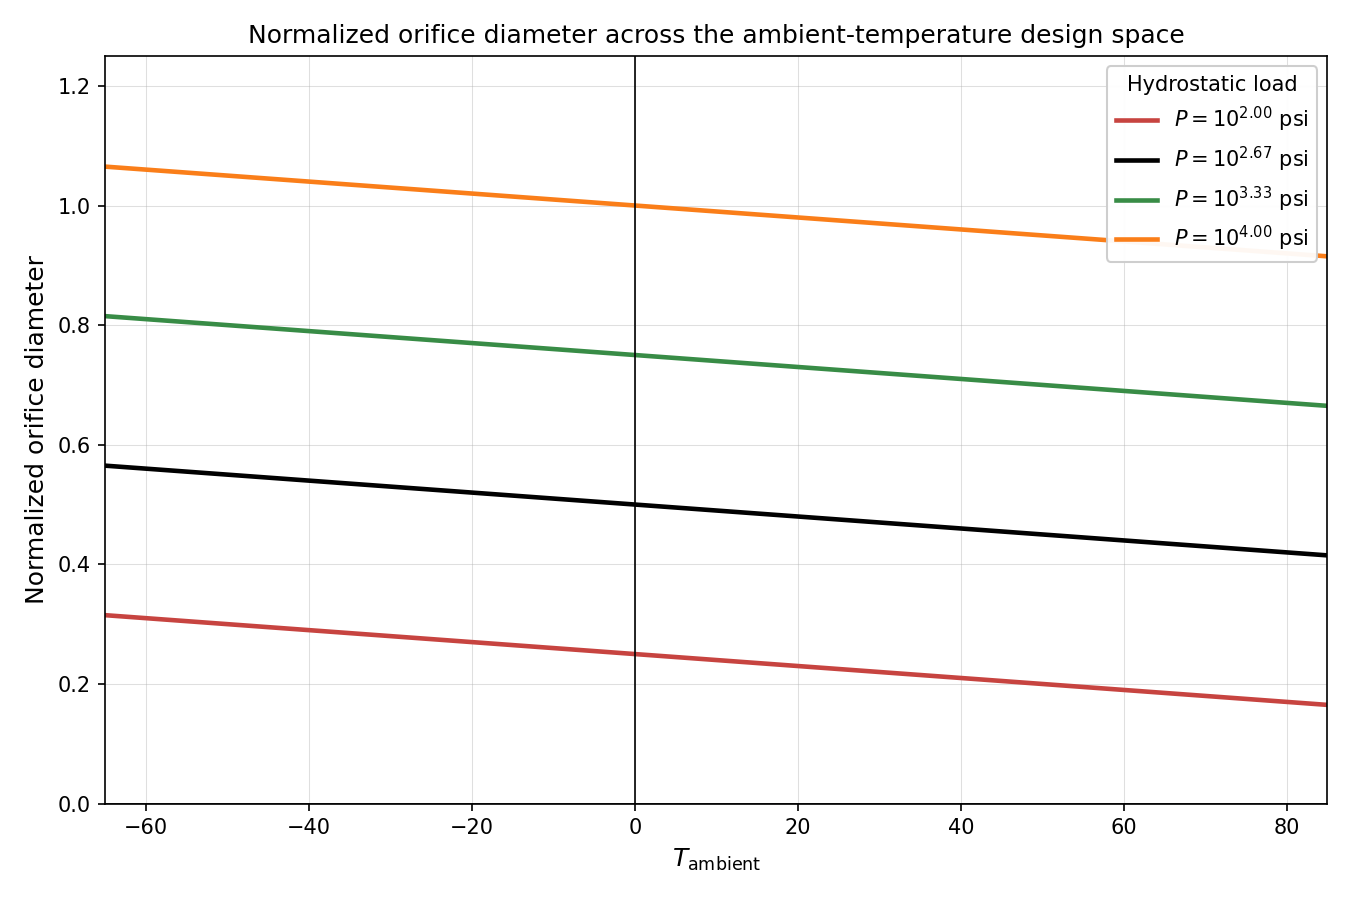
\includegraphics[width=.90\textwidth]{figures3/testingch_designspace.png}
                \caption{Example of a plot that encompasses the entire design space}
                \label{fig:designspace}
\end{figure}
The design space explored by the computational prototype can be summarized by
recovering data from the simulation software to generate a similar figure to the
one above. The four lines in the figure are part of a family of lines in the
design space. The vertical axis is the orifice diameter normalized with the
orifice diameter at the maximum pressure of 10000 psi at an ambient temperature
of 0 C.


	\subsubsection{Data Collection}
	Surface data will be collected on weld joints and failure points identified by
	DFMEA. These data can be recovered at any point in the PTCD as shown in fig \ref{fig:stressnstrain}.
	\begin{figure}[h]
			\centering
			\begin{subfigure}[t]{0.45\textwidth}
					\centering
					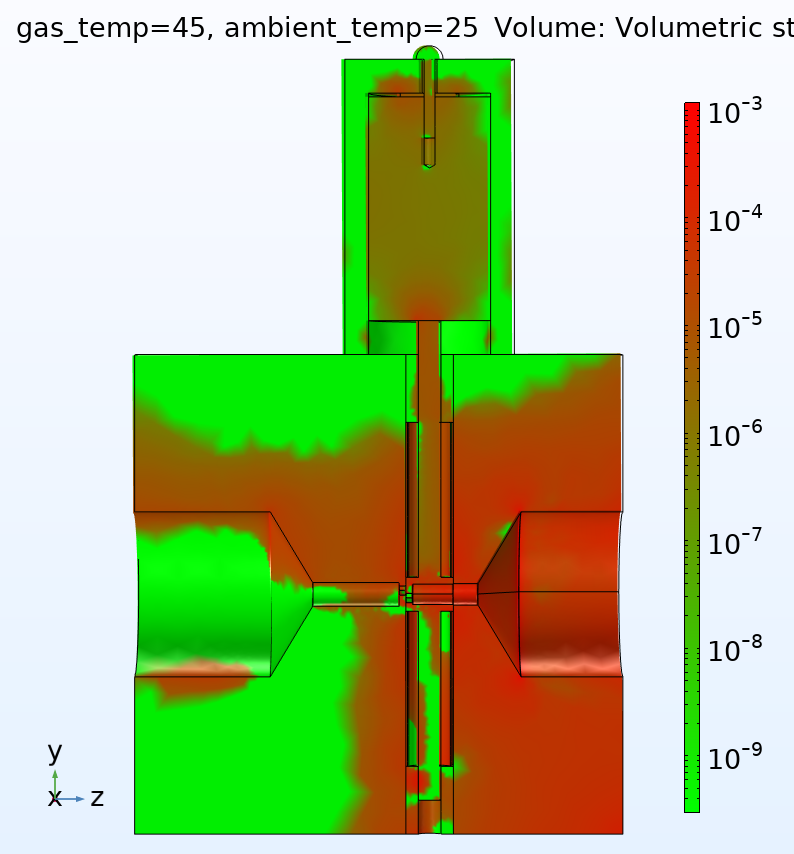
\includegraphics[width=\textwidth]{figures3/testing_ch_volstrain.png}
					\caption{Volumetric strain}
					\label{fig:straindata}
			\end{subfigure}
			\begin{subfigure}[t]{0.45\textwidth}
					\centering
					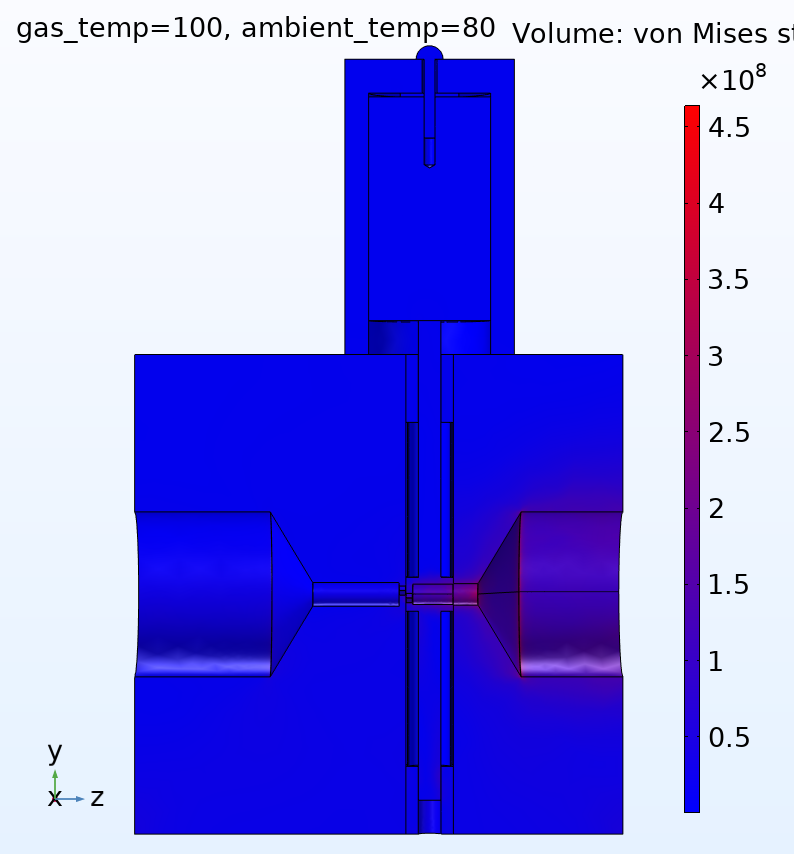
\includegraphics[width=\textwidth]{figures3/testing_ch_volstress.png}
					\caption{Von-Misses Stress}
					\label{fig:stressdata}
			\end{subfigure}
			\caption{Stress and strain map}
			\label{fig:stressnstrain}
	\end{figure}
	\subsubsection{Limitations}
	Several simplifications were introduced to the multi-body simulation to prioritize numerical convergence and reduce overall geometric complexity. 
	Contact friction between interacting surfaces was omitted from the model entirely. 
	To bypass the heavy computational cost of meshing, the Inconel bellows were represented using an equivalent material model rather than their true physical geometry. 
	Similarly, the screw and washer were modeled as a continuous union rather than discrete interactive components. The Allvar component was approximated with an isotropic coefficient of thermal expansion based on nominal textbook values, which inherently neglects the alloy's true anisotropic thermal behavior.

	\section{Results}


	\subsection{Other relevant results/Discussion}

	\subsubsection{Heat Transfer}
	The stationary parametric sweep converged across the full \SI{-60}{\celsius} to
	\SI{80}{\celsius} operating range and reproduced the analytical stroke model.
	The two FEA anchor points at $\Delta T = \SI{5}{\kelvin}$ and
	$\Delta T = \SI{10}{\kelvin}$ returned actuator displacements of
	\SI{5.58}{\micro\meter} and \SI{11.14}{\micro\meter}, establishing a slope of
	\SI{1.115}{\micro\meter\per\kelvin} and matching the analytical prediction
	within \SI{0.2}{\percent}.

	The time-dependent study, run for a representative \SI{20}{\kelvin} ambient
	step, produced a clean first-order exponential response at the monitored
	actuator point, rising from \SI{25}{\celsius} toward a steady-state plateau of
	approximately \SI{44.8}{\celsius}. The thermal time
	constant was $\tau \approx \SI{500}{\second}$ (about \SI{8}{\minute}), read as
	the time to reach \SI{63}{\percent} of the final rise. The actuator reached
	\SI{95}{\percent} of its final temperature in approximately \SI{25}{\minute} and
	was effectively settled by approximately \SI{50}{\minute}. The single-exponential
	character confirms the device behaves as one dominant thermal mass over this
	step, with no oscillatory or multi-rate dynamics in the relevant range.

	\subsection{Design space}
	\begin{figure}[H]
									\centering
									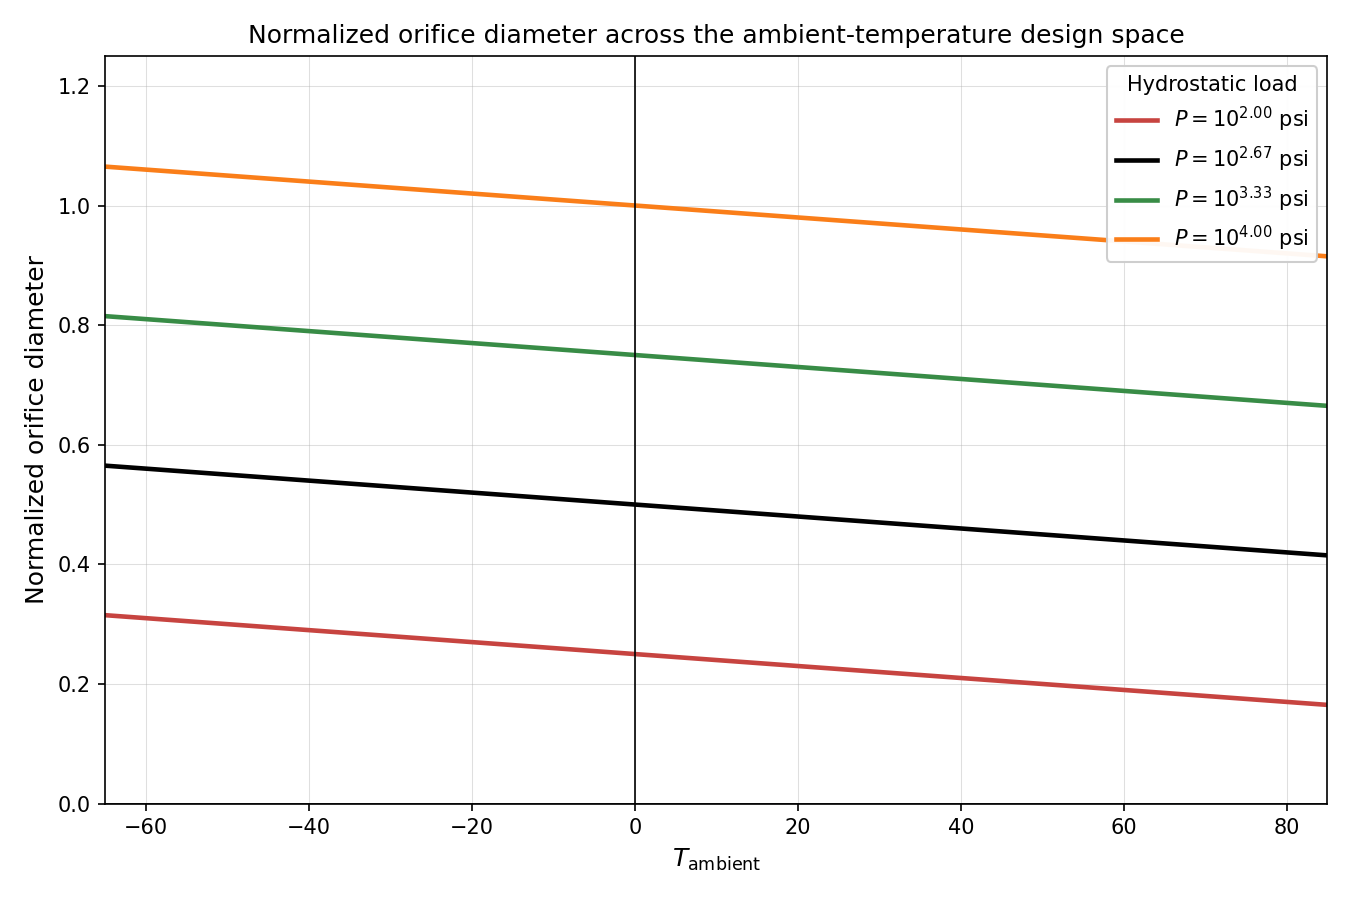
\includegraphics[width=.90\textwidth]{figures3/testingch_designspace.png}
									\caption{Example of a plot that encompasses the entire design space}
									\label{fig:designspace}
	\end{figure}
	The design space explored by the computational prototype can be summarized by
	recovering data from the simulation software to generate a similar figure to the
	one above. The four lines in the figure are part of a family of lines in the
	design space. The vertical axis is the orifice diameter normalized with the
	orifice diameter at the maximum pressure of 10000 psi at an ambient temperature
	of 0 C.


\chapter{Conclusion}
\label{chap:concl}

	The Passive Temperature Compensation Device presented in this design report combines proven, robust technology with a novel valve-orifice architecture
	to accomplish thermomechanical flow control with greater precision than has been achieved before.
	By only allowing flow through the overlap between two diamond holes pressed flush against one another, one mobile and one fixed,
	the \device\ can produce first-order variations in its effective orifice diameter with a single moving part.
	These square holes can be manufactured with very sharp corners using wire EDM (Electric-Discharge Machining).
	An external bimetallic thermal actuator drives these changes with compound mechanical displacement.
	Its interface is hermetically sealed with minimal mechanical or fluid resistance using two flexible metal bellows.
	Specialized materials and precise electron-beam welding maximize thermal stability, strength, and compactness.
	This proof-of-concept model provides Sandia National Laboratories with the necessary design foundation for development of a working physical prototype
	and customization of the design for specific experiments.

	The design process is unfinished. As intended, only the first iteration was fully developed.
	The computational prototype presented in this report demonstrates the feasibility of the \device\ and provides convenient tools for further iteration.
	Appendix~\ref{app:iter:weak} provides an exhaustive list of identified weaknesses and unaddressed assmumptions. In summary, not all error modes could be accounted for in Appendix~\ref{sec:DFMEA:error},
	leading to an optimistic estimation of the device's performance. Full verification will not be complete until Sandia revises this design, builds a physical prototype, and tests it.
	Appendix~\ref{app:iter:customize} provides them with guidance on how to use these computational tools for this revision.

	To assist with this process, the below recommendations identify changes the authors would implement in the second design iteration:

	\begin{enumerate}
		\item Certain dimensions were chosen arbitrarily and over-engineered, leading to excessive safety factors in some places. These values can now be amended to minimize the device's structural margin
			to an industry-standard value, typically 1.5\cite{ref_sf}. These include the thickness of the Mount's upper surface, the height of the Valve Orifice, the contact length of each housing thread,
			the size and thickness of each orifice square, and wall thicknesses around the housing.
		\item The I718-159-72-430 bellows can be replaced with the I718-159-72-2300\cite{ref_miniflex_catalog}, which has a higher squirm and burst rating and \nicefrac{1}{3} the free length with only five times the spring constant.
			The lower bellows can also be eliminated. These would each significantly reduce the height of the \device, by far its longest dimension.
		\item Measures can be taken to eliminate heat transfer. Though the actuator is thermally insulated and separated from the hot internal gas by a thick wall of Invar, this wall should be made thicker to improve its indifference to internal flow conditions.
			Furthermore, the actuator can be reshaped to improve external heat transfer by cutting holes in the mount to expose the internal actuator, weakening its axial strength to increase fidelity to the ambient air temperature.
			This can be taken further, cutting fins into the actuator structure (typically done with wire EDM as with the orifice holes) to maximize convection.
		\item The mount would be better attached to the housing using fasteners due to the difficulty of welding dissimilar metals. If sealed properly, fasteners would provide a reliable permanent attachment
			and could afford alternate calibration architectures, such as the use of precision shims.
		\item The mount and actuator core can trade materials, using an Aluminum mount and an ALLVAR core. This would require repositioning of the leading orifice, which can be easily done such that it is positioned above the fixed orifice;
			it would significantly reduce the cost of the actuator subsystem (Aluminum is far cheaper than ALLVAR and would be better suited for the larger-diameter part) and would more readily enable manipulation of its geometry as described in the previous two items.
		\item Finally, the screw may interfere with the thermal expansion of the actuator. This can be solved by using a shorter screw or one made of Aluminum to match the actuator's expansion rate.
			An ALLVAR screw may be harder to procure if the actuator materials are reversed.
	\end{enumerate}

	Many of these design changes would degrade system performance, risking failure to meet the Required Relationship in equation~\ref{eq:required_relationship}.
	Many other priorities, such as size and cost considerations, were sacrificed to maximize the \device's ability to reach this narrow tolerance window.
	However, using the computational tools presented in Chapter~\ref{chap:test}, a more informed trade-off analysis can determine the real impact of these changes, as is further detailed in Appendix~\ref{app:iter:customize}.

	This first-iteration design of the \device\ demonstrates feasibility as a high-precision thermomechanical valve. Once revised, prototyped, and tested by Sandia, it can provide reliable, passive experimental flow regulation without depending on external power or computation,
	streamlining experimental control and improving the accuracy and repeatability of their research.

	% \begin{itemize}
	% 	\item The actuator is assumed to be fused to the mount's upper interior surface, defined by the plane of the belleville washer's underside, from which it can freely expand.
	% 		In reality, the screw, washer, and mount material along the washer's vertical dimension will interfere with this expansion in slight ways that have not been modeled.
	% 	\item Rotational precision of each diamond hole was assumed to be exact. In reality, the EDM cut may include a slight unquantified tilt, whose error is too involved for calculation in this report.
	% 	\item The Valve Orifice is assumed to be flush against the Housing Outlet, held by its sliding fit and upstream pressure. Any gas that leaks through the orifice by passing around the sides of the moving plate
	% 		will nullify the device's precision control. This failure mode could not be sufficiently analyzed, but measures may need to be taken to prevent flow around the Valve Orifice.
	% 		A flexible metal bellows could be attached between the Housing Inlet and the Valve Orifice that moves sideways as the valve stem oscillates; this would complicate the design but ensure all gas enters the Valve Orifice;
	% 		additional measures would be required to ensure gas does not leak from the interface between the leading and trailing orifice.
	% 	\item The \device's design nomenclature is ambiguous. Certain part names --- namely, the Valve Orifice and Actuator --- are easily confused with the actual diamond-overlap orifice and the actuator assembly, respectively.
	% 		These should be revised before further development.
	% 	\item As mentioned in Section~\ref{subsubsec:design:just:gen_dim:ME}, certain dimensions can be optimized to decrease the Mechanical Envelope if necessary.
	% 		The verification tools developed in Chapter~\ref{chap:DFMEA} provide a convenient method to quantify the impact of these changes on system output precision.
	% 		\begin{itemize}
	% 			\item The lower bellows may not be necessary. It guards against unbalanced pressure force on the underside of the Valve Orifice, being transferred to the actuator, which may be stiff enough to
	% 				withstand this force.
	% 			\item Similarly, the bellows could be replaced with the I718-159-72-2300\cite{ref_miniflex_catalog}, which has a higher squirm and burst rating and \nicefrac{1}{3} the free length of the I718-159-72-430
	% 				but five times the spring constant. The bellows was selected primarily for its low spring constant, but the spring force was eventually found to be negligible.
	% 			\item The thread-contact length can be shortened. These values were not optimized due to their large margin along the longitudinal mechanical envelope.
	% 			\item The top of the mount can be made thinner to shorten the actuator. So can the noncritical housing walls, to create a uniform safety factor of just above 1.
	% 		\end{itemize}
	% 	\item Orifice dimensions can also be optimized. The side lengths of each square and, more importantly, the \SI{1}{\milli\meter} thickness of each orifice wall, were arbitrarily chosen to provide easy-to-cut features.
	% 		The manufacturer may be able to cut through a thicker material without difficulty.
	% 	\item To save cost, the ALLVAR and aluminum materials can be swapped, allowing for a significantly smaller ALLVAR core than the current mount.
	% 		The assembly would lift the valve stem when heated, but placing the leading orifice above the trailing orifice would accommodate this change. 
	% \end{itemize}

	% Other general weaknesses of the \device\ include the following:

	% \begin{itemize}
	% 	\item The current design assumes connection to a \SI{19.05}{\milli\meter} pipe, which falls within the range provided in Operational Condition~\ref{cond:pipe}, but the design does not readily allow
	% 		for all pipe diameters up to the maximum stipulated limit of \SI{25.4}{\milli\meter}.
	% 		This was an oversight and should be remedied if necessary by adding sufficient material to the housing structure to support the large inner bore.
	% \end{itemize}

% \chapter*{} % Bibliography without extra header
\addcontentsline{toc}{chapter}{Bibliography}

\begin{thebibliography}{99}

	\bibitem{ref_sandiaprompt} % SNL Project Prompt
	B.\ Bon,
	``Passive Temperature Compensation Device --- Project Prompt,''
	Sandia National Laboratories, SAND2025-15446O, 2025. [Unpublished].

	\bibitem{ref_ASHRAE_thermostatic} % Bimetallic thermostatic damper actuators
	R.\ McDowall, \textit{Fundamentals of HVAC Control Systems}, I-P ed.,
	American Society of Heating, Refrigerating and Air-Conditioning Engineers, Atlanta, GA, 2009,
	Sec.~1.2.

	\bibitem{ref_Vernet_1938} % Wax thermostatic actuator (original patent)
	S.\ Vernet, ``Thermostat,'' U.S. Patent 2\,115\,501, Apr.\ 26, 1938.
	Available: \url{https://patents.google.com/patent/US2115501}
	[Accessed: May 11, 2026].

	\bibitem{ref_Bugby_2021} % ALLVAR-aluminum thermal switch
	D.\ C.\ Bugby, J.\ G.\ Rivera, S.\ L.\ Mauro, and J.\ T.\ Farmer,
	``Extended Stroke and Miniaturized Reverse-Operation DTE Thermal Switches,''
	\textit{50th Int.\ Conf.\ on Environmental Systems}, ICES-2021-412, Jul.\ 2021.

	\bibitem{ref_Ralphs_2024} % ALLVAR-aluminum thermal switch
	M.\ Ralphs, M.\ Sinfield, M.\ Jensen, and M.\ Felt,
	``Passive Cryogenic Thermal Switch with Tunable Close Temperature for Redundant Cryocooler Systems,''
	\textit{Cryocoolers 23}, R.~G. Ross, Jr. and J.~R. Raab, Eds., International Cryocooler Conference, Inc., Boulder, CO, 2024, pp.~389--394.

	\bibitem{ref_Ralphs_2026} % ALLVAR-aluminum thermal switch
	M.\ I.\ Ralphs, M.\ Jensen, A.\ Eames, and M.\ Sinfield,
	``A Suite of Thermal Switches for Surviving Extreme Thermal Environments in Space,''
	\textit{AIAA SciTech 2026 Forum}, Orlando, FL, Jan.\ 2026, doi: 10.2514/6.2026-1086.

	\bibitem{ref_NIH} % Thickness of human hair; compared to tolerance window
	F.-C.\ Yang, Y.\ Zhang, and M.\ C.\ Rheinstädter, ``The Structure of People's Hair,'' \textit{PeerJ}, vol.~2, p.~e619, Oct.\ 2014. doi: 10.7717/peerj.619.

	\bibitem{ref_NASA_specs_guide} % Systems Engineering Requirement and Specification Strategies
	National Aeronautics and Space Administration, \textit{NASA Systems Engineering Handbook}, NASA/SP-2016-6105 Rev2,
	Washington, DC: NASA, 2016, Sec.~4.2.

	\bibitem{ref_Nise} % Controls and Transfer Functions
	N. S. Nise, Control Systems Engineering, 8th ed. Hoboken, NJ: Wiley, 2019.

	\bibitem{ref_Invar_1897} % Discovery of Invar 36 by Charles Édouard Guillaume, in French
	C.-\'{E}.\ Guillaume, ``Recherches sur les aciers au nickel. Dilatations aux temp\'{e}ratures \'{e}lev\'{e}es; r\'{e}sistance \'{e}lectrique,'' \textit{Comptes Rendus de l'Acad\'{e}mie des Sciences}, vol.~125, pp.~235--238, 1897.

	\bibitem{ref_Invar_1920} % Guillaume's Nobel Prize speech, in English
	C.-\'{E}.\ Guillaume, ``Invar and Elinvar,'' Nobel Lecture, Nobel Prize in Physics, Stockholm, Sweden, Dec.\ 11, 1920.
	Available: \url{https://www.nobelprize.org/prizes/physics/1920/guillaume/lecture/}
	[Accessed: May 8, 2026].

	\bibitem{ref_shigley} % Mechanical Design and torque required to compress belleville
	J.~E. Shigley, C.~R. Mischke, and R.~G. Budynas, \textit{Mechanical Engineering Design},
	8th~ed., McGraw-Hill, New York, 2006.

	\bibitem{ref_wilton_hermetic}	% Hermetic Seal secondary source
	D.\ Wilton, ``Hermetic seal,'' \textit{Wordorigins.org}, Dec.\ 29, 2020.
	[Online]. 
	Available: \url{https://www.wordorigins.org/big-list-entries/hermetic-seal}
	[Accessed: Jun.\ 2, 2026].

	\bibitem{ref_gesner_1559}	% Hermetic Seal primary source
	K.\ Gesner, \textit{The Treasure of Euonymus Conteyninge the Wonderfull Hid
	Secretes of Nature}, P.\ Morwyng, trans., London: John Daie, 1559, p.~66.

	\bibitem{ref_Young_Freedman} % Hooke's Law
	H. D. Young and R. A. Freedman, \textit{University Physics with Modern Physics}, 15th ed. Hoboken, NJ: Pearson, 2019, Eq. 6-8.

	\bibitem{ref_miniflex_catalog} % Bellows 2026 catalog
	Mini-Flex Corporation, \textit{2026 Metal Bellows Catalog}, Mini-Flex Corporation, Watervliet, NY. [Online]. Available: \url{https://mini-flex.com/metal-bellows-catalog/}
	[Accessed: Feb. 23, 2026]

	\bibitem{ref_miniflex_design} % Bellows catalog design guide
	Mini-Flex Corporation, \textit{Metal Bellows Design Guide}, Mini-Flex Corporation, Watervliet, NY. [Online]. Available: \url{https://mini-flex.com/metal-bellows-design-guide/}
	[Accessed: Feb. 23, 2026].

	\bibitem{ref_TiCN_Coating} % TiCN coating properties
	T.~Lv, T.~Luo, T.~Cheng, X.~Hu, Z.~Zhang, Z.~Tang, B.~Lin, and H.~Xiao, 
		``Microstructure and wear behavior of invar alloy surface strengthened by {TiAl} laser alloying and {TiCN} ceramics,'' 
		\emph{Surface and Coatings Technology}, vol. 520, p. 132977, 2026. doi: 10.1016/j.surfcoat.2025.132977.

	\bibitem{ref_steen2010laser} % Laser weld guide
	W. M. Steen and J. Mazumder, \textit{Laser Material Processing}, 4th ed., 
	Springer, London, UK, 2010.

	\bibitem{ref_asme_b313}
	American Society of Mechanical Engineers, \textit{ASME B31.3: Process Piping}, 
	ASME, New York, NY, 2022.

	\bibitem{ref_ashby} % E vs CTE plot
	M.F.\ Ashby, \textit{Materials Selection in Mechanical Design},
	5th ed., Pergamon Press, Oxford, UK, 1992, Fig~3.13.

	\bibitem{ref_NASA_specs_Al} % Al CTE as a funciton of temp, E
		% CTE at room temp = 23.85 ppm/C
		% E = 68.95 MPa
	R.\ F.\ Muraca and J.\ S.\ Whittick, \textit{Materials Data Handbook: Aluminum Alloy 6061}, 2nd ed., Western Applied Research \& Development, Inc., NASA CR-123772, May 1972.

	\bibitem{ref_AllvarAlloys} % ALLVAR CTE, E
		% CTE = -30 ppm/C
		% E = 55 GPa
	ALLVAR Alloys, \textit{What is Negative Thermal Expansion?}, ALLVAR Alloys, 2026. [Online]. Available: \url{https://allvaralloys.com/negative-coefficient-of-thermal-expansion-products-applications/round-bar-and-tube/}
	[Accessed: May 8, 2026].

	\bibitem{ref_AllvarAlloys_gen} % ALLVAR Alloys homepage
	ALLVAR Alloys, \textit{Negative Thermal Expansion. Positive Results.} ALLVAR Alloys, 2026. [Online]. Available: \url{https://www.allvaralloys.com/}
	[Accessed: May 9, 2026].

	\bibitem{ref_Carpenter_Inv} % Invar 36 CTE, E
		% CTE = 1.3 ppm/C
		% E = 141 GPa
	Carpenter Technology Corporation, \textit{Invar 36 Datasheet}, Carpenter Technology Corporation, 2025. [Online]. Available: \url{https://www.carpentertechnology.com/hubfs/7407324/Material%20Saftey%20Data%20Sheets/Invar%2036.pdf}
	[Accessed: May 8, 2026].

	\bibitem{ref_Carpenter_gen} % Holds the registered trademark for the name Invar 36; this is their homepage
	Carpenter Technology Corporation, \textit{Global Leader in Specialty Alloys}, Carpenter Technology Corporation, 2026. [Online]. Available: \url{https://www.carpentertechnology.com/}
	[Accessed: May 8, 2026].

	\bibitem{ref_ASM_Steel} % Used for CTE comparison
		% CTE = 11.7 ppm/C
		F. Cverna, Ed., \textit{ASM Ready Reference: Thermal Properties of Metals}, ASM International, Materials Park, OH, 2002, Table~2.2.

	\bibitem{ref_SpecialMetals_Inc} % Inconel CTE, E
		% CTE = 13.2 ppm/C
		% E = 200 GPa
	Special Metals Corporation, \textit{INCONEL\textregistered{} Alloy 718}, Publication No. SMC-045, Special Metals Corporation, 2007. [Online]. Available: \url{https://www.specialmetals.com/documents/technical-bulletins/inconel/inconel-alloy-718.pdf}
	[Accessed: Apr. 17, 2026].

	\bibitem{ref_SpecialMetals_gen} % Holds the registered trademark for the name INCONEL 718; this is their homepage
	Special Metals Corporation, \textit{High-Performance Alloy Products}, Special Metals Corporation, 2026. [Online]. Available: \url{https://www.specialmetals.com/}
	[Accessed: May 8, 2026].

	\bibitem{ref_Inconel_1965} % Discovery of Inconel 718 by Herbert Louis Eiselstein 
	H.~L. Eiselstein, ``Metallurgy of a Columbium-Hardened Nickel-Chromium-Iron Alloy,'' in \textit{Advances in the Technology of Stainless Steel and Related Alloys},
	ASTM Special Technical Publication 369, American Society for Testing and Materials, Philadelphia, 1965, pp.~62--79.

	\bibitem{ref_Inconel_1991} % Eiselstein's reflection on the discovery of Inconel 718 at a conference
	H.~L. Eiselstein and D.~J. Tillack,``The Invention and Definition of Alloy 625,'' in \textit{Superalloys 718, 625 and Various Derivatives},
	E.~A. Loria, Ed., The Minerals, Metals \& Materials Society, Warrendale, PA, 1991, pp.~1--14.

	\bibitem{ref_NASA_Inc} % Inconel advantages
	J.~A. Lee, \textit{Hydrogen Embrittlement}, NASA Technical Memorandum NASA/TM-2016-218602,
	NASA Marshall Space Flight Center, Huntsville, AL, 2016.

	\bibitem{ref_McMaster_belle} % belleville washer part specificaitons
	McMaster-Carr, \textit{[316 Stainless Steel Spring Lock Washer], Part No. 93237A101}, McMaster-Carr Supply Company, 2026. [Online]. Available: \url{https://www.mcmaster.com/93237A101/}
	[Accessed: May 8, 2026].

	\bibitem{ref_din6796} % Standard for belleville washer
	Deutsches Institut f\"{u}r Normung, \textit{DIN 6796: Conical Spring Washers for Bolted Connections}, DIN, Berlin, 2009.

	\bibitem{ref_dinen16983} % Referenced by DIN 6796
	Deutsches Institut f\"{u}r Normung, \textit{DIN EN 16983: Disc Springs---Calculation}, DIN, Berlin, 2017.

	\bibitem{ref_dinen16984} % Referenced by DIN 6796
	Deutsches Institut f\"{u}r Normung, \textit{DIN EN 16984: Disc Springs---Quality Specifications---Dimensions}, DIN, Berlin, 2017.

	\bibitem{ref_almen1936} % Referenced by DIN 16983
	Almen, J.~O. and Laszlo, A., ``The Uniform-Section Disk Spring,''
	\textit{Transactions of the American Society of Mechanical Engineers}, vol.~58, no.~4, pp.~305--314, 1936.

	\bibitem{ref_Ledbetter_Stainless} % 304 and 316 Stainless Steel E, poisson at 20C
		% 18-8 304 SS:
			% E = 210.1 GPa
			% ν = 0.279
		% 316 SS:
			% E = 207.8 GPa
			% E = 0.282
	Ledbetter, H.~M., ``Stainless-Steel Elastic Constants at Low Temperatures,'' \textit{Journal of Applied Physics}, vol.~52, no.~3, pp.~1587--1589, 1981.

	\bibitem{ref_jones1992}
	L.A.\ Jones, I.W.\ Hunter, R.J.\ Irwin,
	``Differential thresholds for limb movement measured using adaptive techniques,''
	\textit{Perception \& Psychophysics}, vol.~52, no.~5, pp.~529--535, 1992.

	\bibitem{ref_desrosieres2015}
	P.\ Marini, L.\ Masia, G.\ Morasso, et~al.,
	``Robot-aided assessment of wrist proprioception,''
	\textit{Frontiers in Human Neuroscience}, vol.~9, article~198, 2015.

	\bibitem{ref_SNL} % Sandia About Page
	Sandia National Laboratories, \textit{About Sandia}, Sandia National Laboratories, 2026. [Online]. Available: \url{https://www.sandia.gov/about/}
	[Accessed: May 30, 2026].

	\bibitem{ref_Jensen} % Numerical Methods and Taylor Series
	N. Grønbech-Jensen, Introduction to Numerical Methods and Analysis.
	[Unpublished]

	\bibitem{ref_Stewart} % Calculus and Taylor Series
	J. Stewart, Single Variable Calculus: Early Transcendentals, 6th ed. Belmont, CA: Thomson Brooks/Cole, 2008, p. 736; see also p. 674

	\bibitem{ref_Hibbeler} % Mechanics of Materials: thermal expansion, material spring constant
	R. C. Hibbeler, Mechanics of Materials, 9th ed. Saddle River, NJ: Pearson, 2014.

	\bibitem{ref_beam}
	A. Grishin, ``Thin-Wall Rectangular Pressure Vessels Simulation,'' Phoenix Analysis \& Design Technologies (PADT), Inc., Tempe, AZ, USA, White Paper, Jun. 30, 2024. Available: \url{https://www.padtinc.com/wp-content/uploads/2024/06/thinwall_rectangular_pressure_vessels.pdf}. [Accessed: May 29, 2026].

	\bibitem{ref_COMSOL} % COMSOL Multiphysics simulation software
	COMSOL~AB, \textit{COMSOL Multiphysics\textregistered{} Reference Manual},
	v.~5.3a, COMSOL~AB, Stockholm, Sweden, 2017.

	\bibitem{ref_Anton} % Linear Algebra and Linear Dependency
	H. Anton and A. Kaul, \textit{Elementary Linear Algebra}, 12th ed.
	Hoboken, NJ: Wiley, 2019, p. 228.

	\bibitem{ref_figliola}
	R.\ S.\ Figliola and D.\ E.\ Beasley,
	\textit{Theory and Design for Mechanical Measurements},
	5th~ed., Wiley, Hoboken, NJ, 2011, Sec.~4.9.

	\bibitem{ref_AIAG2005}
	Automotive Industry Action Group (AIAG),
	\textit{Statistical Process Control (SPC) Reference Manual},
	2nd~ed., AIAG, Southfield, MI, 2005, p.~104,132.

	\bibitem{ref_white}
		F.\ M.\ White and H.\ Xue,
		\textit{Fluid Mechanics}, 9th~ed.,
		McGraw-Hill Education, New York, NY, 2021.

	\bibitem{ref_haas} % HAAS tolerance for drawings
	Haas Automation, Inc., ``VF-2: 40-Taper Standard Vertical Mill Specifications,'' \textit{Haas Automation}. [Online]. Available: \url{https://www.haascnc.com/machines/vertical-mills/vf-series/models/small/vf-2.html}.
	[Accessed: May 16, 2026].

	\bibitem{ref_McMaster_screw} % M2 screw part specificaitons
	McMaster-Carr, \textit{[18-8 Stainless Steel Pan Head Torx Screws], Part No. 90362A141}, McMaster-Carr Supply Company, 2026. [Online]. Available: \url{https://www.mcmaster.com/90362A141/}
	[Accessed: May 8, 2026].

	\bibitem{ref_McMaster_std} % Standard washer part specificaitons
	McMaster-Carr, \textit{[18-8 Stainless Steel General Purpose Washer], Part No. 93475A195}, McMaster-Carr Supply Company, 2026. [Online]. Available: \url{https://www.mcmaster.com/93475A195/}
	[Accessed: May 8, 2026].

	\bibitem{ref_sf}
	U.S.\ Department of Defense,
	\textit{MIL-STD-1522A: Standard General Requirements for Safe Design and
	Operation of Pressurized Missile and Space Systems},
	Department of Defense, Washington, DC, 1984, Table~III.

\end{thebibliography}


\newpage
\begin{appendices}
\appendix

\chapter{Calculations and Supplemental Information}
\label{app:calcs}

	\section{Required Relationship: Tolerable Error}
	\label{app:calcs:errorProp}

		As detailed in Section~\ref{sec:intro:req}, the Required Relationship

			$$ \requiredRelationship $$

		depends on the following independent variables, each with their own tolerance values:

			\begin{align*}
				&A_1 = \Aone
				\\
				&A_0 = \Azero
			\end{align*}

		The tolerance of $D_{\text{effective}}$ as a function of temperature can be found using the following formula:

			\begin{equation}
				D_{\text{eff}} = \overline{D_{\text{eff}}}(T) \pm u_D(T)
				\label{eq:error_gen}
			\end{equation}

		where

			\begin{equation}
				u_D(T) =
				\begin{cases}
					- (5 \%) A_1 (T - T_{ref}) + (5 \%) A_0 & T \geq T_{ref} \\
					 (5 \%) A_1 (T - T_{ref}) + (5 \%) A_0 & T < T_{ref}
				\end{cases}
				\label{eq:error_particular}
			\end{equation}

		Because $A_1 < 0$ and the sign of $T - T_{ref}$ changes at $T = T_{ref}$, the $A_1$ error term must be reversed for higher temperatures.
		Combining equations \eqref{eq:error_gen} and \eqref{eq:error_particular}, we find the range allowed by the Required Relationship across the whole temperature spectrum, represented in Table~\ref{tab:RR} and Figure~\ref{fig:RR}.

		\begin{table}[H]
			\centering
			\caption{Required Relationship $D = A_1 (T - T_{ref}) + A_0$ for $\SI{-60}{\degreeCelsius} \leq T \leq \SI{80}{\degreeCelsius}$}
			\label{tab:RR}
			\begin{tabular}{ccc}
				\toprule
				$T$ (\textdegree C) & $D$ (\si{\micro\meter}) & $u_D$ (\si{\micro\meter}) \\
				\midrule
				$-60$ & 383.5 & 19.18 \\
				$-50$ & 368.3 & 18.42 \\
				$-40$ & 353.1 & 17.65 \\
				$-30$ & 337.8 & 16.89 \\
				$-20$ & 322.6 & 16.13 \\
				$-10$ & 307.3 & 15.37 \\
				$0$   & 292.1 & 14.61 \\
				$10$  & 276.9 & 13.84 \\
				$20$  & 261.6 & 13.08 \\
				$25$  & 254.0 & 12.70 \\
				$30$  & 246.4 & 13.08 \\
				$40$  & 231.1 & 13.84 \\
				$50$  & 215.9 & 14.61 \\
				$60$  & 200.7 & 15.37 \\
				$70$  & 185.4 & 16.13 \\
				$80$  & 170.2 & 16.89 \\
				\bottomrule
			\end{tabular}
		\end{table}

		\vspace{1em}
		\begin{figure}[H]
			\centering
			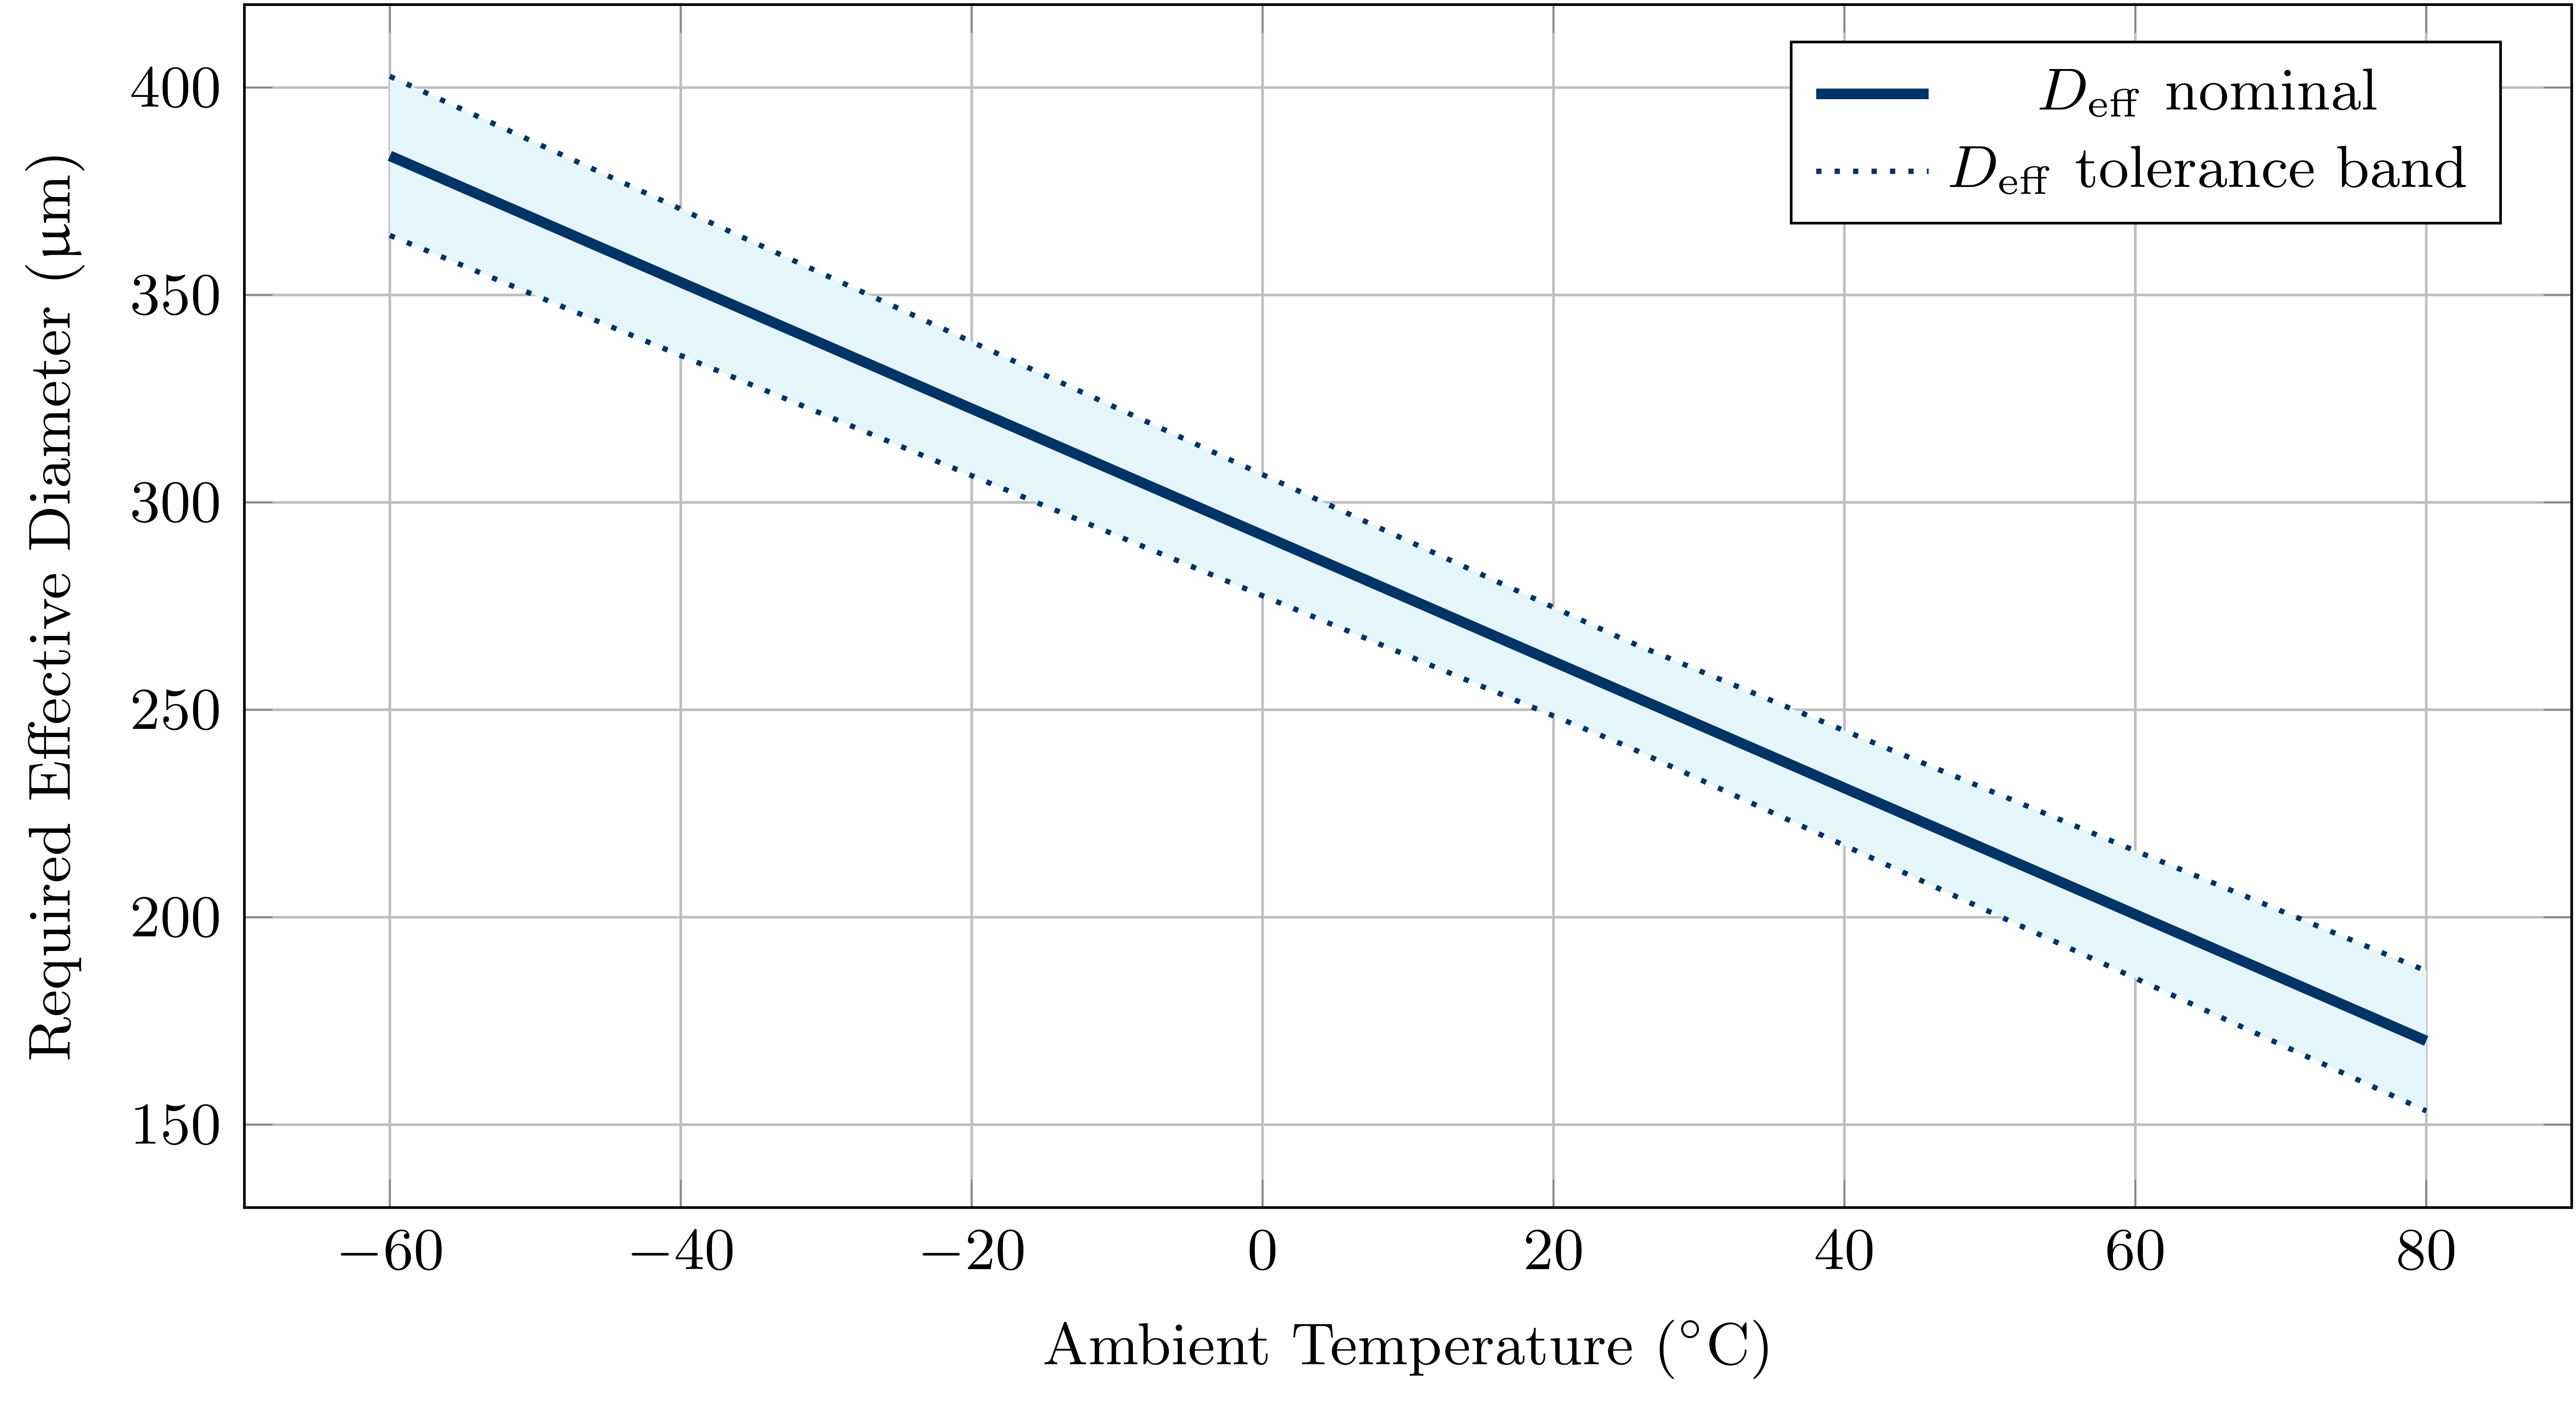
\includegraphics[width=\textwidth]{RR.png}
			\caption{Required Relationship tolerance window}
			\label{fig:RR}
		\end{figure}

		Observe that the error boundary is thinnest about $T_{ref}$; thus, performance is best served if the \device\ is manufactured, assembled, and calibrated near this temperature.
		See Appendix~\ref{app:mfg} for more details.

	\section{Final Design Specifications}
	\label{app:calcs:specs}

		Table~\ref{tab:specs} compiles the full set of design specifications developed in Section~\ref{sec:intro:specs}.

		\begin{table}[h]
			\centering
			\caption{System Requirements and Subsystem Specification Rolldown}
			\renewcommand{\arraystretch}{1.3}
			\begin{tabularx}{\textwidth}{
					>{\raggedright\arraybackslash}p{0.04\textwidth}  % R ID
					>{\raggedright\arraybackslash}X                  % Requirement
					>{\raggedright\arraybackslash}p{0.06\textwidth}  % V ID
					>{\raggedright\arraybackslash}X                  % Valve spec
					>{\raggedright\arraybackslash}p{0.06\textwidth}  % A ID
					>{\raggedright\arraybackslash}X                  % Actuator spec
			}
			\toprule
			\textbf{} & \textbf{System Requirements} &
			\textbf{} & \textbf{Valve Specifications} &
			\textbf{} & \textbf{Actuator Specifications} \\
			\midrule

			% Row 1
			\multirow{3}{=}{\vspace{10em}R.1} & \multirow{3}{=}{\ReqA} &
			V.1.1 & \SpecVAA &
			A.1.1 & \SpecAAA \\

			& & V.1.2 & \SpecVAB \SpecVABapp & A.1.2 & \SpecAAB \\

			\midrule

			% Row 2
			R.2 & \ReqB &
			V.2.1 & \SpecVB &
			A.2.1 & \SpecAB \\
			
			\midrule

			% Row 3
			\multirow{3}{=}{\vspace{10em}R.3} & \multirow{3}{=}{\ReqC} &
			V.3.1 & \SpecVCA &
			\multirow{3}{=}{\vspace{10em}A.3.1} & \multirow{3}{=}{\SpecACA} \\

			& & V.3.2 & \SpecVCB & & \\

			& & V.3.3 & \SpecVCC & & \\

			\bottomrule
			\end{tabularx}
			\label{tab:specs}
		\end{table}

	\section{Orifice Geometry}
	\label{app:calcs:orifice_geometry}

		The orifice, as defined in Section~\ref{sec:design:overview} and depicted in Figure~\ref{fig:orifice} (shown again in Figure~\ref{fig:orifice_rep}), is the ``Venn''-style overlap between two angled squares.

		\begin{figure}[H]
			\centering
			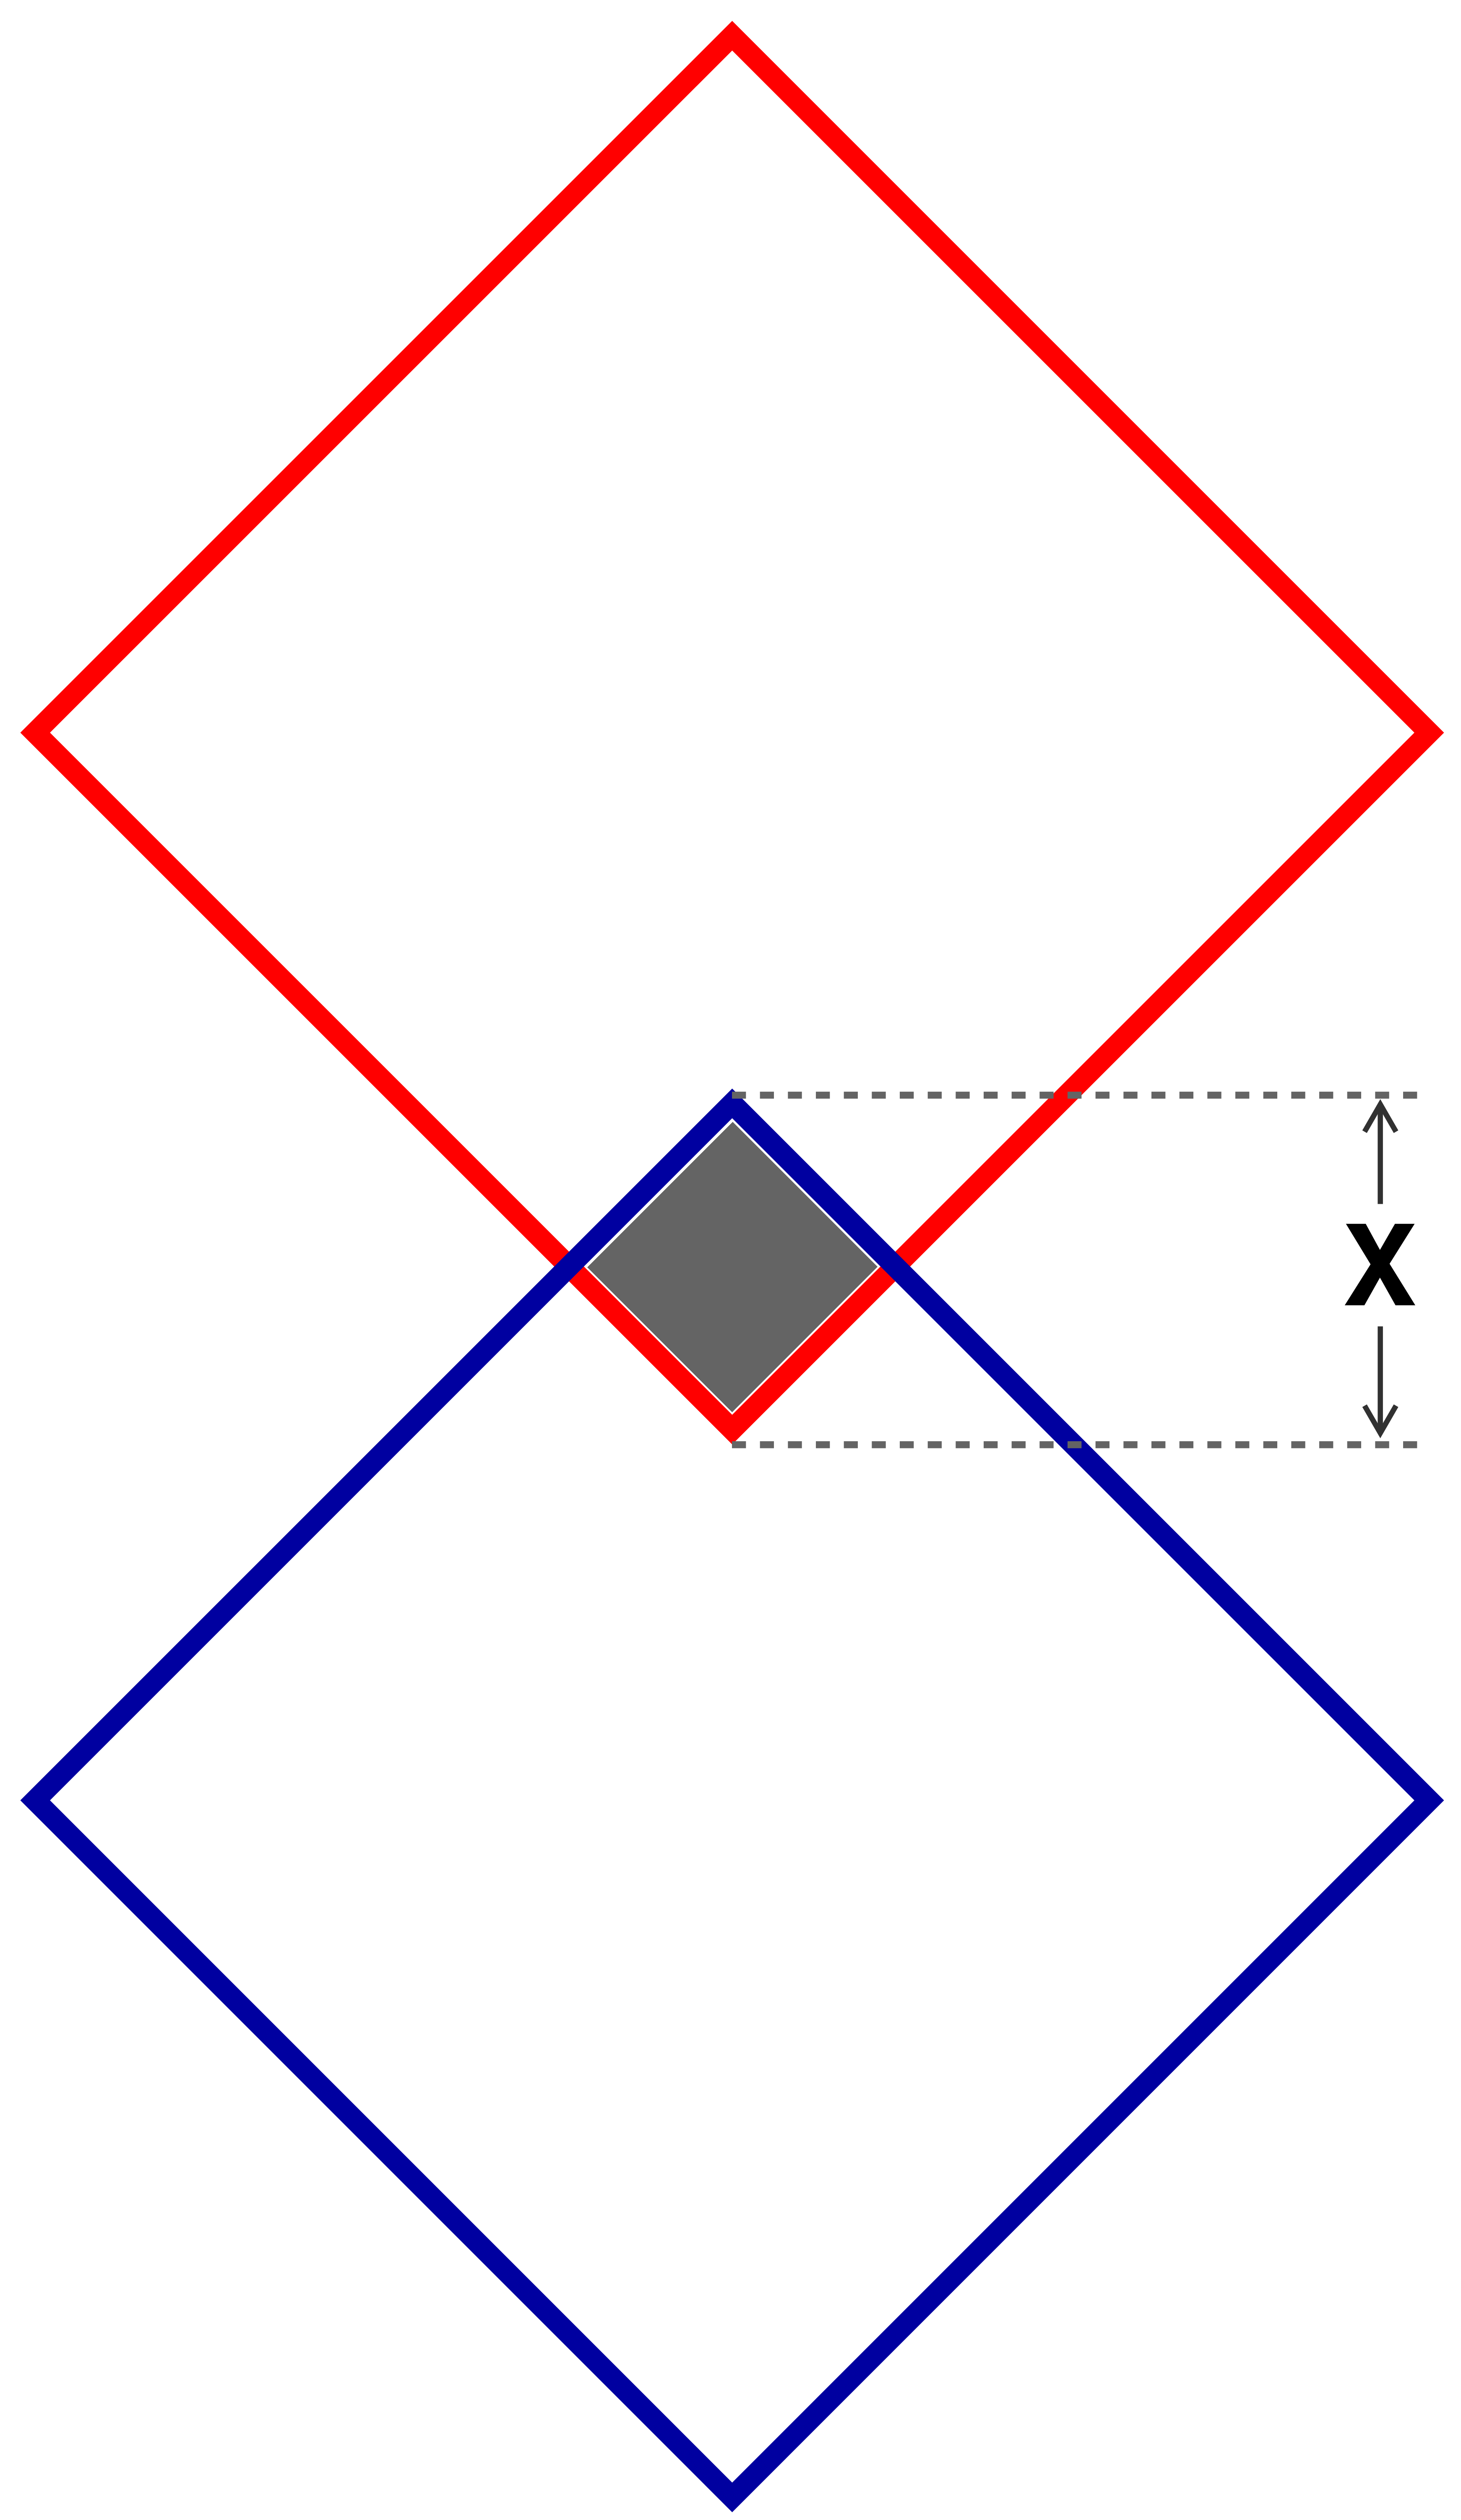
\includegraphics[height=2in]{orifice_app.png}
			\caption{Orifice geometry, repeated}
			\label{fig:orifice_rep}
		\end{figure}

		\begin{figure}[H]
			\centering
			
\includegraphics[height=2in]{orifice_detailed.png}
			\caption{Orifice geometry, detailed}
			\label{fig:orifice_detailed}
		\end{figure}

		The effective diameter of an orifice of any geometry is the diameter of a circle with equivalent area, such that
		
		\begin{equation}
			A = \frac{\pi}{4}D_{\text{effective}}^2
			\label{eq:d_eff}
		\end{equation}

		Thus, the height of the orifice X as defined in Figures \ref{fig:orifice_rep} and \ref{fig:orifice_detailed}, which is directly driven by the actuator movement, 
		can be related to the effective diameter as follows:

		\begin{align}
			A &= \frac{\pi}{4}D_{\text{eff}}^2 = s^2 \\
			s &= \sqrt{\frac{\pi}{4}}D_{\text{eff}} \\
			X &= \sqrt{s^2 + s^2} = \sqrt{2}s \text{ by the Pythagorean Theorem}
		\end{align}

		Therefore,

			\begin{equation}
				X = \sqrt{2}\sqrt{\frac{\pi}{4}}D_{\text{eff}} = \sqrt{\frac{\pi}{2}}D_{\text{eff}}
			\end{equation}

		Finally, we can rearrange this relation to obtain the effective diameter as a function of X:

			\begin{equation}
				D_{eff} = \sqrt{\frac{2}{\pi}} X
			\end{equation}

	\section{System Calibration}
	\label{app:calcs:cal}
	
		\subsection{Belleville Washer Reaction Force}
		\label{app:calcs:cal:force}

			The belleville washer that separates the two cylinders of the actuator (A1 and A2), purchased from McMaster Carr\cite{ref_McMaster_belle}, applies a spring force as it is clamped by the screw during the calibration process.
			According to the material data listed by McMaster, characteristic properties of the belleville washer are defined by the \textit{Deutsches Institut für Normung} (DIN; German Institute for Standardization), standard 6796\cite{ref_din6796},
			which cites DIN EN 16983\cite{ref_dinen16983} and 16984\cite{ref_dinen16984} for their spring properties. DIN EN\footnote{i.e. European Norm} 16984 in turn cites a 1936 paper by Almen and Laszlo\cite{ref_almen1936}, which provides the below calculation for the washer's reaction force per deflection.
			This design report assumes a deflection of \SI{50}{\micro\meter} and, if all parts are machined and assembled as specified within tolerance, the applied deflection will be near this value.
			However, the washer can deflect up to \SI{200}{\micro\meter} if necessary.
			The following force is required to apply a deflection within this range during calibration:

			\vspace{1em}
			\begin{table}[H]
				\centering
				\caption{Belleville Washer (part 93237A101) Specifications\cite{ref_McMaster_belle, ref_Ledbetter_Stainless}}
				\label{tab:belle}
				\begin{tabular}{lll}
					\toprule
					Parameter & Variable & Value \\
					\midrule
					Outer Diameter    & $OD$          & \SI{5}{\milli\meter} \\
					Inner Diameter    & $ID$          & \SI{2.2}{\milli\meter} \\
					Young's Modulus   & $E$           & \SI{207.8}{\giga\pascal} \\
					Poisson's Ratio   & $\nu$         & $0.282$ \\
					Free Height       & $H$           & \SI{0.6}{\milli\meter} \\
					Thickness         & $t$           & \SI{0.4}{\milli\meter} \\
					Cone Height       & $h = H - t$   & \SI{0.2}{\milli\meter} \\
					Deflection        & $\delta$      & $0 \leq \delta \leq \SI{0.2}{\milli\meter}$ \\
					\bottomrule
				\end{tabular}
			\end{table}

			\begin{align}
					\text{Diameter Ratio } \alpha &= \frac{OD}{ID} \\
					\text{Load Constant } M &= \frac{6}{\pi \ln(\alpha)} \left( \frac{\alpha - 1}{\alpha} \right)^2 \\
					\text{Load } P &= \frac{E \delta}{(1 - \nu^2) M \frac{OD^2}{4}} \left[ \left( h - \delta \right) \left( h - \frac{\delta}{2} \right) t + t^3 \right]
			\end{align}

			From these, we obtain the expected force value

			\begin{equation}
				P(\SI{50}{\micro\meter}) = \SI{184}{\newton}
			\end{equation}

			The required torque to apply this load is defined in Shigley's Mechanical Engineering Design\cite[Eq.~8-27, Table~8-15]{ref_shigley}:

			\begin{equation}
				T = K F d = (0.18) (\SI{184}{\newton}) (\SI{2}{\milli\meter})
			\end{equation}

			where

			\begin{align*}
				&K \text{ is the nut factor (assuming Loctite is applied,} \\
				&\text{which is recommended in the Manufacturing Guide - Appendix~\ref{app:mfg})} \\
				&F \text{ is the reaction load} \\
				&d \text{ is the diameter of the M2 screw}
			\end{align*}
			
			yielding an expected torque of \SI{6.6e-2}{\newton\meter} at the \SI{50}{\micro\meter} compression, a very reasonable value for an M2 screw.

			Figures \ref{fig:belle_force} and \ref{fig:belle_torque} show the calculated load and required torque across the whole compression range.

			\begin{figure}[H]
				\centering
				\begin{tikzpicture}
					\begin{axis}[
						width=12cm,
						height=7cm,
						xlabel={Deflection $\delta$ (\si{\micro\meter})},
						ylabel={Load $P$ (N)},
						xmin=0, xmax=201,
						ymin=0,
						grid=major,
						grid style={dashed, gray!40},
						tick align=outside,
					]
						\addplot[blue, thick, no marks]
							table[col sep=comma, x index=0, y index=1] {csv/F.csv};
					\end{axis}
				\end{tikzpicture}
				\caption{Belleville washer reaction force}
				\label{fig:belle_force}
			\end{figure}

			\vspace{1em}
			\begin{figure}[H]
				\centering
				\begin{tikzpicture}
					\begin{axis}[
						width=12cm,
						height=7cm,
						xlabel={Deflection $\delta$ (\si{\micro\meter})},
						ylabel={Torque $T$ (N$\cdot$m)},
						xmin=0, xmax=201,
						ymin=0,
						grid=major,
						grid style={dashed, gray!40},
						tick align=outside,
					]
						\addplot[red, thick, no marks]
							table[col sep=comma, x index=0, y index=2] {csv/F.csv};
					\end{axis}
				\end{tikzpicture}
				\caption{Torque required to tighten the screw as it compresses the belleville washer}
				\label{fig:belle_torque}
			\end{figure}

		\subsection{Achievable Error Correction}
		\label{app:calcs:cal:sat}

			As discussed in Section~\ref{app:sat:TF:results}, this calibration stack will occasionally be necessary to correct static machine dimension errors,
			whose expected range falls a maximum of \SI{30.7}{\micro\meter} above and \SI{44.6}{\micro\meter} below the nominal value.
			The belleville washer's maximum deflection is equal to its free cone height

			\begin{equation}
				h = H - t = \SI{200}{\micro\meter}
			\end{equation}

			From the assumed compression of \SI{50}{\micro\meter}, the \device\ can be calibrated to an effective diameter decrease of \SI{50}{\micro\meter} and an increase of

			\begin{equation}
				\SI{200}{\micro\meter} - \SI{50}{\micro\meter}
			\end{equation}

			Thus, to properly account for all linear error possibilities, the calibration assembly must be able to adjust $D_{eff}$ by no less than \SI{44.6}{\micro\meter}.
			The belleville washer's total compressible range is the difference between its free cone height and its thickness.
			As shown in its specification drawing in Appendix~\ref{app:datasheets:McMaster}, this results in a total deflection height of

			\begin{equation}
				\SI{0.6}{\milli\meter} - \SI{0.4}{\milli\meter} = \SI{200}{\micro\meter}
			\end{equation}

			To reliably bring the system into tolerance, the user must be able to precisely adjust the output in increments no more than the narrowest tolerance window, found at $T_{ref}$.

			\begin{equation}
				D_{eff}(T_{ref}) = 254.0 \pm \SI{12.7}{\micro\meter} \rightarrow 2 \cdot \SI{12.7}{\micro\meter} = \SI{25.4}{\micro\meter} \text{ total resolution}
			\end{equation}

			Calibration with a resolution no more than \SI{25.4}{\micro\meter} precision will theoretically be able to achieve some setpoint within the tolerable range.
			Let us assume half this value is necessary to be safe and determine whether the assembly can reasonably perform a repeatable \SI{12.7}{\micro\meter} adjustment.

			Calibration adjustment directly translates to changes in the orifice height $X$. We will assume that the orifice height-diameter relation derived in Appendix~\ref{app:calcs:orifice_geometry} holds true,
			as fillet-radius and horizontal-position errors do not consistently affect the diameter across the full temperature range and thus cannot be reliably eliminated by calibration;
			therefore the compression value $X$ translates to changes in the effective diameter according to the relation

			\begin{equation}
				X = \sqrt{\frac{\pi}{2}} D_{eff}
			\end{equation}

			therefore a \SI{12.7}{\micro\meter} change in $D_{eff}$ translates to a \SI{15.9}{\micro\meter} vertical movement.
			Calibration is performed with the M2 screw 90362A141 from McMaster (specification drawing given in Appendix~\ref{app:datasheets:McMaster}),
			whose thread pitch equals \SI{0.4}{\frac{threads}{\milli\meter}}. Thus, a \SI{360}{\degree} turn of the screw corresponds to a \SI{0.4}{\milli\meter} change in the orifice height, meaning

			\begin{equation}
				\left( \SI{12.7}{\micro\meter} \right) \sqrt{\frac{\pi}{2}} \frac{\SI{360}{\degree}}{\SI{400}{\micro\meter}} = \SI{14.3}{\degree}
			\end{equation}

			A \SI{14}{\degree} rotation is a very reasonable demand for  manual screwdriver\cite{ref_jones1992, ref_desrosieres2015}. As discussed in Section~\ref{app:calcs:cal:force}, this can be performed by hand with little effort,
			allowing for even greater precision.

	% \newpage
	
	\section{Supplemental Information}
	\label{app:calcs:sup}

		\subsection{The \device's role in National Security}
		\label{app:calcs:sup:sec}

			The \device\ plays a very niche role. It controls parameters for experiments used in the development of devices that aid in the development of Sandia National Laboratories' defense-technology projects.
			Figure~\ref{fig:app_SNL} illustrates this division of responsibility and shows how the \device\ impacts its ultimate customer, National Security in the United States of America (USA).

			\vspace{1em}
			\begin{figure}[H]
				\centering
				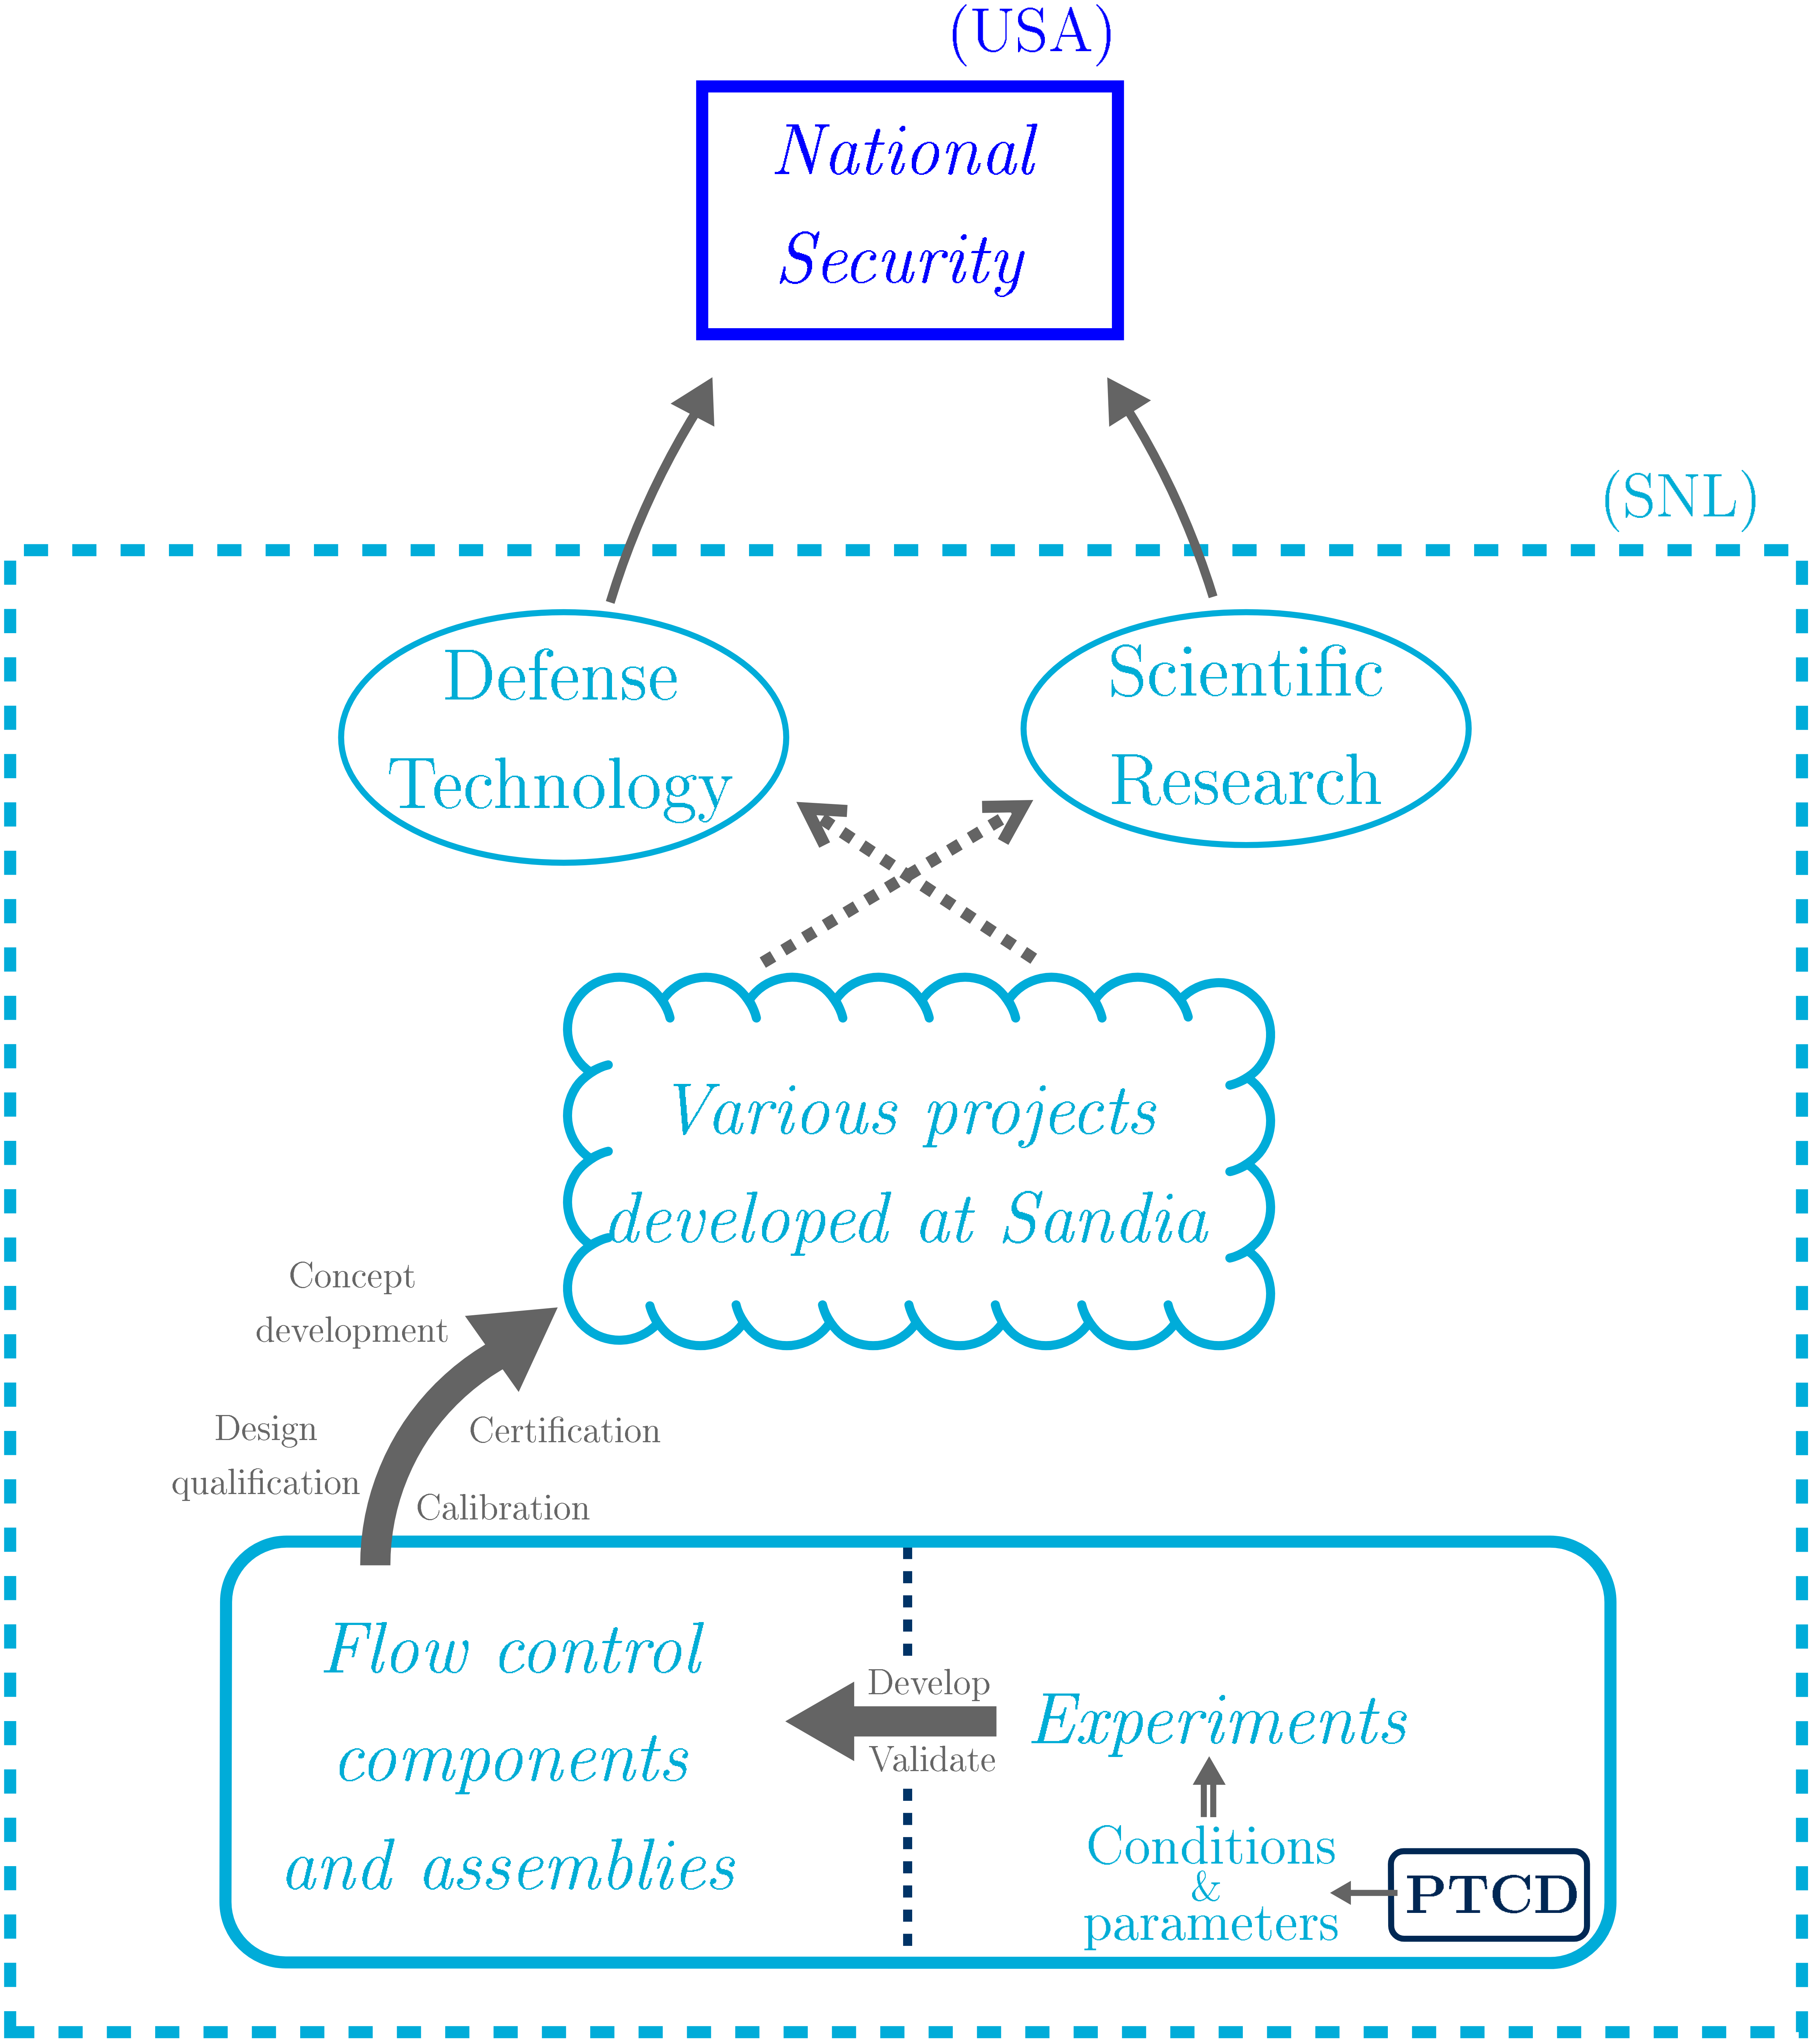
\includegraphics[width=.75\textwidth]{SNL_role.png}
				\caption{Downstream Customer Diagram}
				\label{fig:app_SNL}
			\end{figure}

			As described in Section~\ref{subsec:intro:motive:background}, Sandia National Labs (SNL) develops ``science and technology to resolve the nation's most challenging security issues''\cite{ref_SNL}.
			This consists of various individual projects across a wide range of disciplines, any of which may be impacted by the \device\ and many of which are classified.
			Sandia's Gas Transfer Systems (GTS) team, whose scope is pictured in the lower nested rectangle, develops flow control components and assemblies
			that Sandia then uses for the concept development, design qualification, certification, and calibration of some of their projects.
			GTS develops and validates these components through a series of tightly controlled experiments, often involving the flow of hydrogen or a noble gas, whose sensitive environmental conditions and experimental parameters must be delicately regulated.
			This regulation includes temperature compensation; the \device\ fills this niche. As discussed elsewhere, the effects of temperature fluctuations on the test article must either be mitigated by flow control or dealt with in post-processing by the research engineer.
			The \device\ provides this necessary control without dependence on power or computation, improving the reliability of these experiments, the precision of the flow control components and assemblies, the reliability of Sandia's projects,
			the capabilities of their research and technology, and, ultimately, the resilience of American National Security against ever-more-sophisticated foreign and domestic threats.



		\subsection{The \device\ in full assembly}
		\label{app:calcs:sup:assem}

			Figure~\ref{fig:act_size} shows the actual size of the \device\ when printed on $8 \nicefrac{1}{2}'' \times 11''$ paper.
			Figure~\ref{fig:app_reveal} shows a useful cutaway view of the entire assembly.

			\begin{minipage}{1.5748in}
				\begin{figure}[H]
				\centering
				\includegraphics[width=1.5748in]{act_size.png} % IMPORTANT: Do not change the size of this image. It is printed to-scale.
				\caption{\device\\Actual Size}
				\label{fig:act_size}
				\end{figure}
			\end{minipage}
			\hfill
			\begin{minipage}{6in}
				\begin{figure}[H]
					\centering
					% 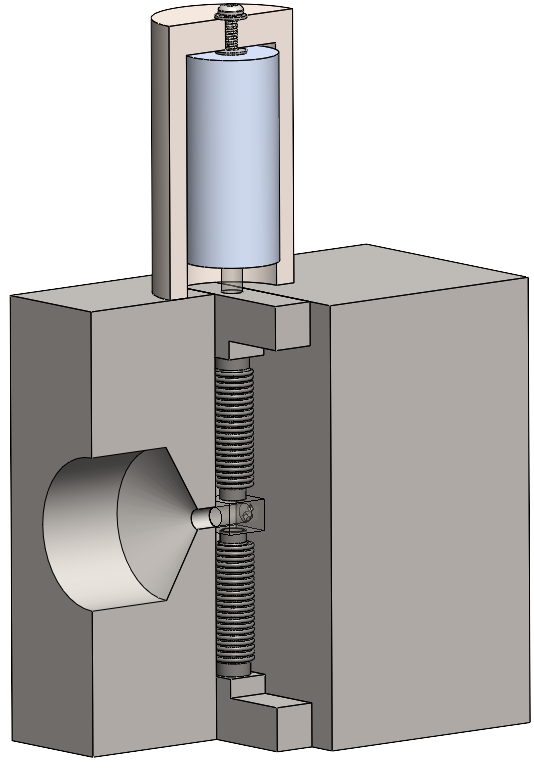
\includegraphics[width=\textwidth]{reveal.png}
					\includegraphics[width=.75\textwidth]{reveal_qual.png}
					\caption{\device\ Full Assembly}
					\label{fig:app_reveal}
				\end{figure}
			\end{minipage}

		\subsection{Noncritical dimensions and features}
		\label{subsec:design:just:gen_dim}

			To design as precise and compact a device as possible, our team deliberated and optimized every dimension and feature. The critical dimensions have been discussed elsewhere.
			Here, other important elements are justified as motivated by our design specifications.

			\subsubsection{Actuator Diameter}
			\label{subsubsec:design:just:gen_dim:act_diam}

				Under the bellows spring reaction force calculated in equation~\eqref{eq:bellow_F}, the actuator and mount are stretched or compressed slightly.
				Like all metals, they act as very stiff springs whose spring constant is proportional to its cross-sectional area.
				Increasing this area minimizes deflection, a source of error.
				The deflection decrease reaches a point of diminishing return near a total outer diameter (OD) of \SI{25}{\milli\meter} (Figure~\ref{fig:mount_OD_opt}).
				This fits well within the actuator's longitudinal and lateral mechanical envelope and reduces the spring deflection to a negligible amount.
				The total deflection is minimized at a mount wall thickness of \SI{3.5}{\milli\meter} (Figure~\ref{fig:mount_thick_opt}).
				It should be no surprise that, as calculated in Sections \ref{app:sat:TF:force_balance:M} and \ref{app:sat:TF:force_balance:A}, their cross-sectional areas are nearly equal at the optimal distribution.
				The decrease of one to increase the other would lead to a net loss in the subsystem spring constant.
				\vspace{1\baselineskip}
				\begin{figure}[H]
					\centering
					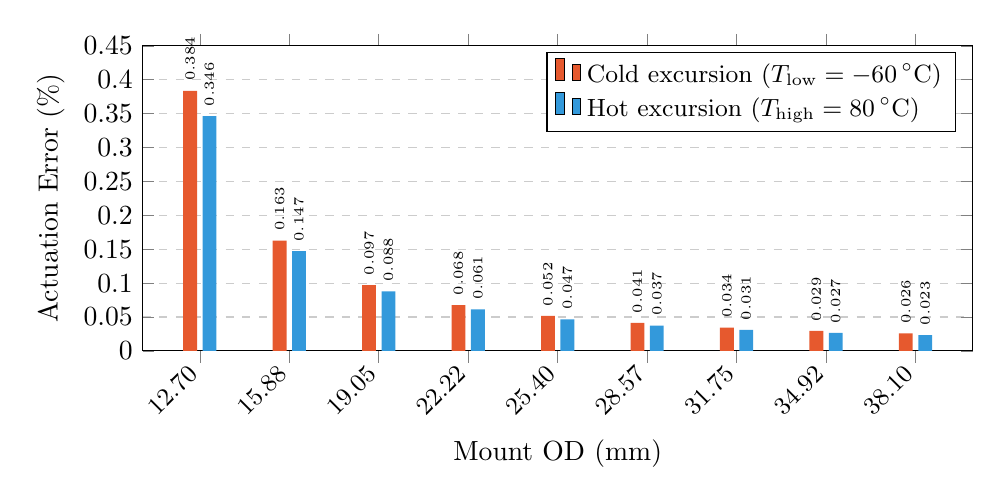
\begin{tikzpicture}
						\begin{axis}[
								ybar,
								bar width=5pt,
								width=\textwidth,
								height=0.45\textwidth,
								xlabel={Mount OD (mm)},
								ylabel={Actuation Error (\%)},
								xtick=data,
								xticklabels={12.70, 15.88, 19.05, 22.22, 25.40, 28.57, 31.75, 34.92, 38.10},
								x tick label style={rotate=45, anchor=east, font=\small},
								legend style={at={(0.98,0.98)}, anchor=north east, font=\small},
								legend cell align={left},
								ymajorgrids=true,
								grid style={dashed, gray!40},
								ymin=0,
								ymax=0.45,
								ytick={0, 0.05, 0.10, 0.15, 0.20, 0.25, 0.30, 0.35, 0.40, 0.45},
								yticklabel={\pgfmathprintnumber[fixed, precision=2]{\tick}},
								enlarge x limits=0.08,
								nodes near coords,
								nodes near coords style={font=\tiny, rotate=90, anchor=west},
								every node near coord/.append style={/pgf/number format/fixed, 
																										/pgf/number format/precision=3},
						]

						%% Hot excursion bars (Design 1) — plotted first
						\addplot[fill={rgb,255:red,230;green,89;blue,46}, draw=none] coordinates {
								(1, 0.3837)
								(2, 0.1628)
								(3, 0.0972)
								(4, 0.0677)
								(5, 0.0515)
								(6, 0.0413)
								(7, 0.0344)
								(8, 0.0294)
								(9, 0.0257)
						};

						%% Cold excursion bars (Design 1) — plotted second
						\addplot[fill={rgb,255:red,51;green,153;blue,219}, draw=none] coordinates {
								(1, 0.3464)
								(2, 0.1470)
								(3, 0.0877)
								(4, 0.0611)
								(5, 0.0465)
								(6, 0.0373)
								(7, 0.0310)
								(8, 0.0266)
								(9, 0.0232)
						};

						\legend{Cold excursion ($T_\text{low}=\SI{-60}{\degreeCelsius}$),
										Hot excursion ($T_\text{high}=\SI{80}{\degreeCelsius}$)}

						\end{axis}
					\end{tikzpicture}
					\caption{Actuator subsystem diameter optimization}
					\label{fig:mount_OD_opt}
				\end{figure}

				\begin{figure}[H]
					\centering
					\pgfplotstableread[col sep=comma]{csv/elastic_deformation.csv}\elasticdata
					\begin{tikzpicture}
						\begin{axis}[
								width=\textwidth,
								height=0.5\textwidth,
								xlabel={Wall thickness (mm)},
								ylabel={Total deflection ($\upmu$m)},
								xmin=0, xmax=12,
								ymin=0, ymax=1.0,
								ytick={0, 0.2, 0.4, 0.6, 0.8, 1.0},
								restrict y to domain=0:1.0,
								xtick={0,1,...,12},
								ymajorgrids=true,
								grid style={dashed, gray!40},
								legend style={
										at={(0.98,0.98)},
										anchor=north east,
										font=\small,
										cells={anchor=west}
								},
								clip=true,
						]

						%% Allvar tube (mount)
						\addplot[
								color={rgb,255:red,46;green,115;blue,178},
								mark=*,
								mark size=2.5pt,
								line width=1.5pt,
						] table[x=t_wall_mm, y=d_alv_max_um] {\elasticdata};
						\addlegendentry{Allvar tube (mount)}

						%% Al rod (actuator)
						\addplot[
								color={rgb,255:red,217;green,84;blue,26},
								mark=square*,
								mark size=2.5pt,
								line width=1.5pt,
						] table[x=t_wall_mm, y=d_al_max_um] {\elasticdata};
						\addlegendentry{Al rod (actuator)}

						%% Combined series
						\addplot[
								color={rgb,255:red,33;green,140;blue,33},
								mark=diamond*,
								mark size=3pt,
								line width=1.5pt,
						] table[x=t_wall_mm, y=d_ser_max_um] {\elasticdata};
						\addlegendentry{Combined series}

						%% Optimal wall thickness vertical line at 3.5 mm
						\draw[dashed, black, line width=1.2pt] (axis cs:3.5, 0) -- (axis cs:3.5, 1.0);

						%% Minimum point marker at (3.5, 0.1401)
						\addplot[
								only marks,
								mark=*,
								mark size=4pt,
								color=black,
						] coordinates {(3.5, 0.140052)};
						\addlegendentry{Series min @ $t_{\text{wall}} = \SI{3.5}{\milli\meter}$}

						\end{axis}
					\end{tikzpicture}
					\caption{Mount wall thickness optimization}
					\label{fig:mount_thick_opt}
				\end{figure}

			\subsubsection{Threaded Interface}
			\label{subsubsec:design:just:gen_dim:thread}

				As detailed by Sandia, gas will be supplied by a stainless steel pipe between \SI{1.524}{\milli\meter} and \SI{25.4}{\milli\meter} in diameter.
				This design features a \SI{19.05}{\milli\meter} (\nicefrac{3}{4}'') threaded interface, which diameter can be adjusted in further design iterations as needed for particular experiments.

				The housing inlet and outlet provide \SI{15}{\milli\meter} and \SI{20}{\milli\meter} threaded length, respectively, for an airtight seal.
				Adding the space needed for the tapered drill-bit cut and the walls that support the valve orifice, the valve subsystem's longitudinal mechanical envelope totals \SI{72}{\milli\meter}, well within its design specification.

				\subsubsection{Assemblability Considerations}
			\label{subsubsec:design:just:gen_dim:assem}

				Manufacture and assembly of the \device\ motivated several features. The full assembly process is detailed in Appendix~\ref{app:mfg}.
				Every weld operation requires an orthogonal beam at all times.
				The housing center is broken into two pieces, allowing the bellows to be welded to the valve orifice and the housing centers separately with a full 360$^\circ$ line of sight.
				The subassembly can then be inserted into the housing inlet and welded in place from above, then fit to the housing outlet and welded from the outside.
				The actuator expansion rod is attached to the valve stem with a 360$^\circ$ weld.
				This is screwed to the mount, which is then welded to the housing.
				This modular approach allows for full line-of-sight welding and simple assembly and drove many of the structural features of the \device.

			\subsubsection{Valve Orifice Contact Friction}
			\label{subsubsec:design:just:gen_dim:friction}

			The interface between vertical faces of the valve orifice and the housing inlet are subject to frictional forces that could cause wear and galling (i.e. degradation of materials as their surfaces slide against one another), which could damage the system performance over time.
			To mitigate this, the contact surfaces are coated with a thin layer of Titanium Carbonitride (TiCN), a hard ceramic coating that provides excellent wear resistance and low friction properties.
			Compared to uncoated Invar, the TiCN coating provides a $5.6\!\times\!$ increase in hardness and a 63\% reduction in the wear rate under similar conditions\cite{ref_TiCN_Coating}.
			The coating is applied using Physical Vapor Deposition (PVD), a process that deposits a thin film $(\approx 2-4 \si{\micro\meter})$ of material onto the surface of the substrate.
			The coated surface are depicted in the Drawing Package in Appendix~\ref{app:drawings}.

			\subsubsection{Mechanical Envelope Specifications}
			\label{subsubsec:design:just:gen_dim:ME}

				As stated in various sections above, each subsystem met its mechanical envelope specifications, with one exception: the valve subsystem violates its vertical mechanical envelope, pushing the total system height to $(\SI{45.55}{\milli\meter} + \SI{70.72}{\milli\meter}) = \SI{116.27}{\milli\meter}$, a 16\% violation of the required mechanical envelope.
				This was necessary to allow a direct interface between the actuator and valve subsystems, dramatically increasing the system precision compared to the complex mechanism required to make it more compact.
				As described in detail in Appendix~\ref{app:PM}, Sandia confirmed the precedence of the Required Relationship over the Mechanical Envelope,
				which is consistent with the system requirement obligation keywords emphasized in Section~\ref{sec:intro:req}.

				A few design changes, discussed in Section~\ref{chap:concl}, may allow the \device\ to fit within the Mechanical Envelope.
				These would slightly sacrifice precision. The impact of these changes could not be reliably evaluated during the initial design process,
			but the tools since developed and presented in Appendix~\ref{app:sat:TF} readily allow for a more informed trade-off analysis.



	\section{Additional Testing Data}
	\label{app:calcs:test}

		\todo{Description}

		\begin{table}[H]
		\centering
		\caption{Actuator stroke across the operating range from the isolated thermal
		model ($\delta = 1.115\,\Delta T$). Boldface rows are the converged FEA anchor
		points that establish the slope; all rows lie on the linear law confirmed by the
		full converged sweep.}
		\label{tab:stroke_full}
		\begin{tabular}{rrr}
		\toprule
		$T_{env}$ (\si{\celsius}) & $\Delta T$ (\si{\kelvin}) & Stroke (\si{\micro\meter}) \\
		\midrule
		$-60$ & $-85$ & $94.78$ \\
		$-50$ & $-75$ & $83.62$ \\
		$-40$ & $-65$ & $72.47$ \\
		$-30$ & $-55$ & $61.33$ \\
		$-20$ & $-45$ & $50.17$ \\
		$-10$ & $-35$ & $39.02$ \\
		$0$   & $-25$ & $27.88$ \\
		$10$  & $-15$ & $16.73$ \\
		$20$  & $-5$  & $5.58$  \\
		$25$  & $0$   & $0.00$  \\
		\textbf{30} & \textbf{5}  & \textbf{5.58}  \\
		\textbf{35} & \textbf{10} & \textbf{11.14} \\
		$40$ & $15$ & $16.73$ \\
		$50$ & $25$ & $27.88$ \\
		$60$ & $35$ & $39.02$ \\
		$70$ & $45$ & $50.17$ \\
		$80$ & $55$ & $61.33$ \\
		\bottomrule
		\end{tabular}
		\end{table}

	\begin{figure}[htbp]
                \centering
                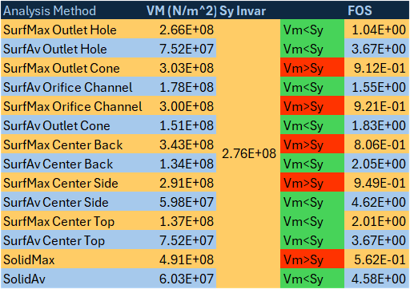
\includegraphics[width=.75\textwidth]{figures3/Orifice Channel FEA.png}
                \caption{Table of Von Mises stresses extracted from the single body FEA of the orifice channel opening.}
                \label{fig:FEAdisp2}
            \end{figure}


\chapter{Required Relationship Failure Analysis}
\label{app:sat}

	Section~\ref{sec:DFMEA::tol} introduces the most important failure consideration: satisfaction of the Required Relationship to the required tolerance as stipulated by equation~\eqref{eq:required_relationship}:

	\begin{equation}
		\requiredRelationship
	\end{equation}

	The below analysis provides a thorough analysis of the effect of several key sources of error and analytically evaluates the final expected output of the \device.

	\section{Error Analysis}
	\label{app:sat:error}

		\subsection{Actuator Coefficient of Thermal Expansion}
		\label{app:sat:error:CTE}

			Typical material specifications list a single coefficient of thermal expansion (CTE).
			However, this value changes slightly as temperature changes, variation which must be accounted for where possible.
			NASA studied the behavior of aluminum across a wide temperature range and found its CTE as a function of temperature, presented in Figure~\ref{fig:al_alpha} \cite{ref_NASA_specs_Al}.
		
			\begin{figure}[h]
				\centering
				\fbox{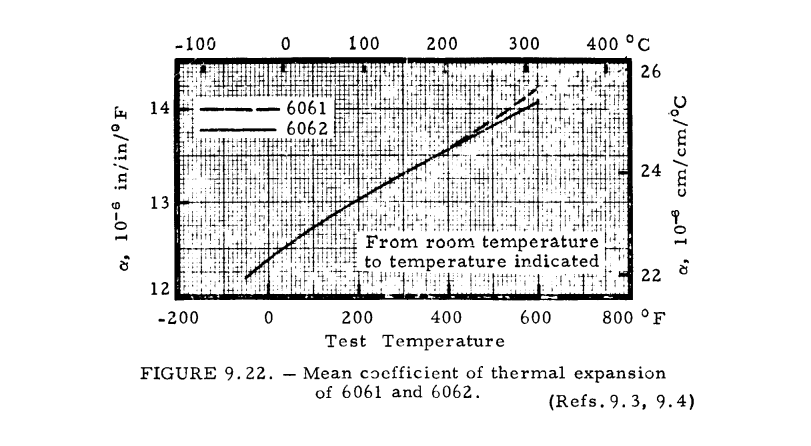
\includegraphics[width=0.8\textwidth]{Al_alpha_values}}
				\caption{Coefficient of thermal expansion of aluminum as a function of temperature}
				\label{fig:al_alpha}
			\end{figure}
			
			Though no numerical data was provided, the temperature-dependent aluminum CTE values can be approximated from this graph, shown in Table~\ref{tab:CTE_Al} in the Appendix.
			From this, we obtain the reference-temperature CTE (\specActuatorCTE) used in Chapter~\ref{chap:design},
			but the true value varies between \SI{21.8}{\micro\meter\per\meter\per\degreeCelsius} and \SI{23.5}{\micro\meter\per\meter\per\degreeCelsius} as $\Tcold \leq T \leq \Thot$.
			These introduce nonlinear behavior, resulting in quantifiable error.

		\subsection{Machine Tolerances}
		\label{app:sat:error:mach}

			General machine dimension tolerances depend on the capabilities of the manufacturing devices available.
			It is reasonable to assume that Sandia's tolerance capabilities meet or exceed those of standard Computer-Numerical Control (CNC) mills.
			The values represented in the engineering drawings (Appendix~\ref{app:drawings}) are taken from HAAS VF-2 series specifications \cite{ref_haas}.

			\begin{wrapfigure}{l}{.4\textwidth}
				\centering
				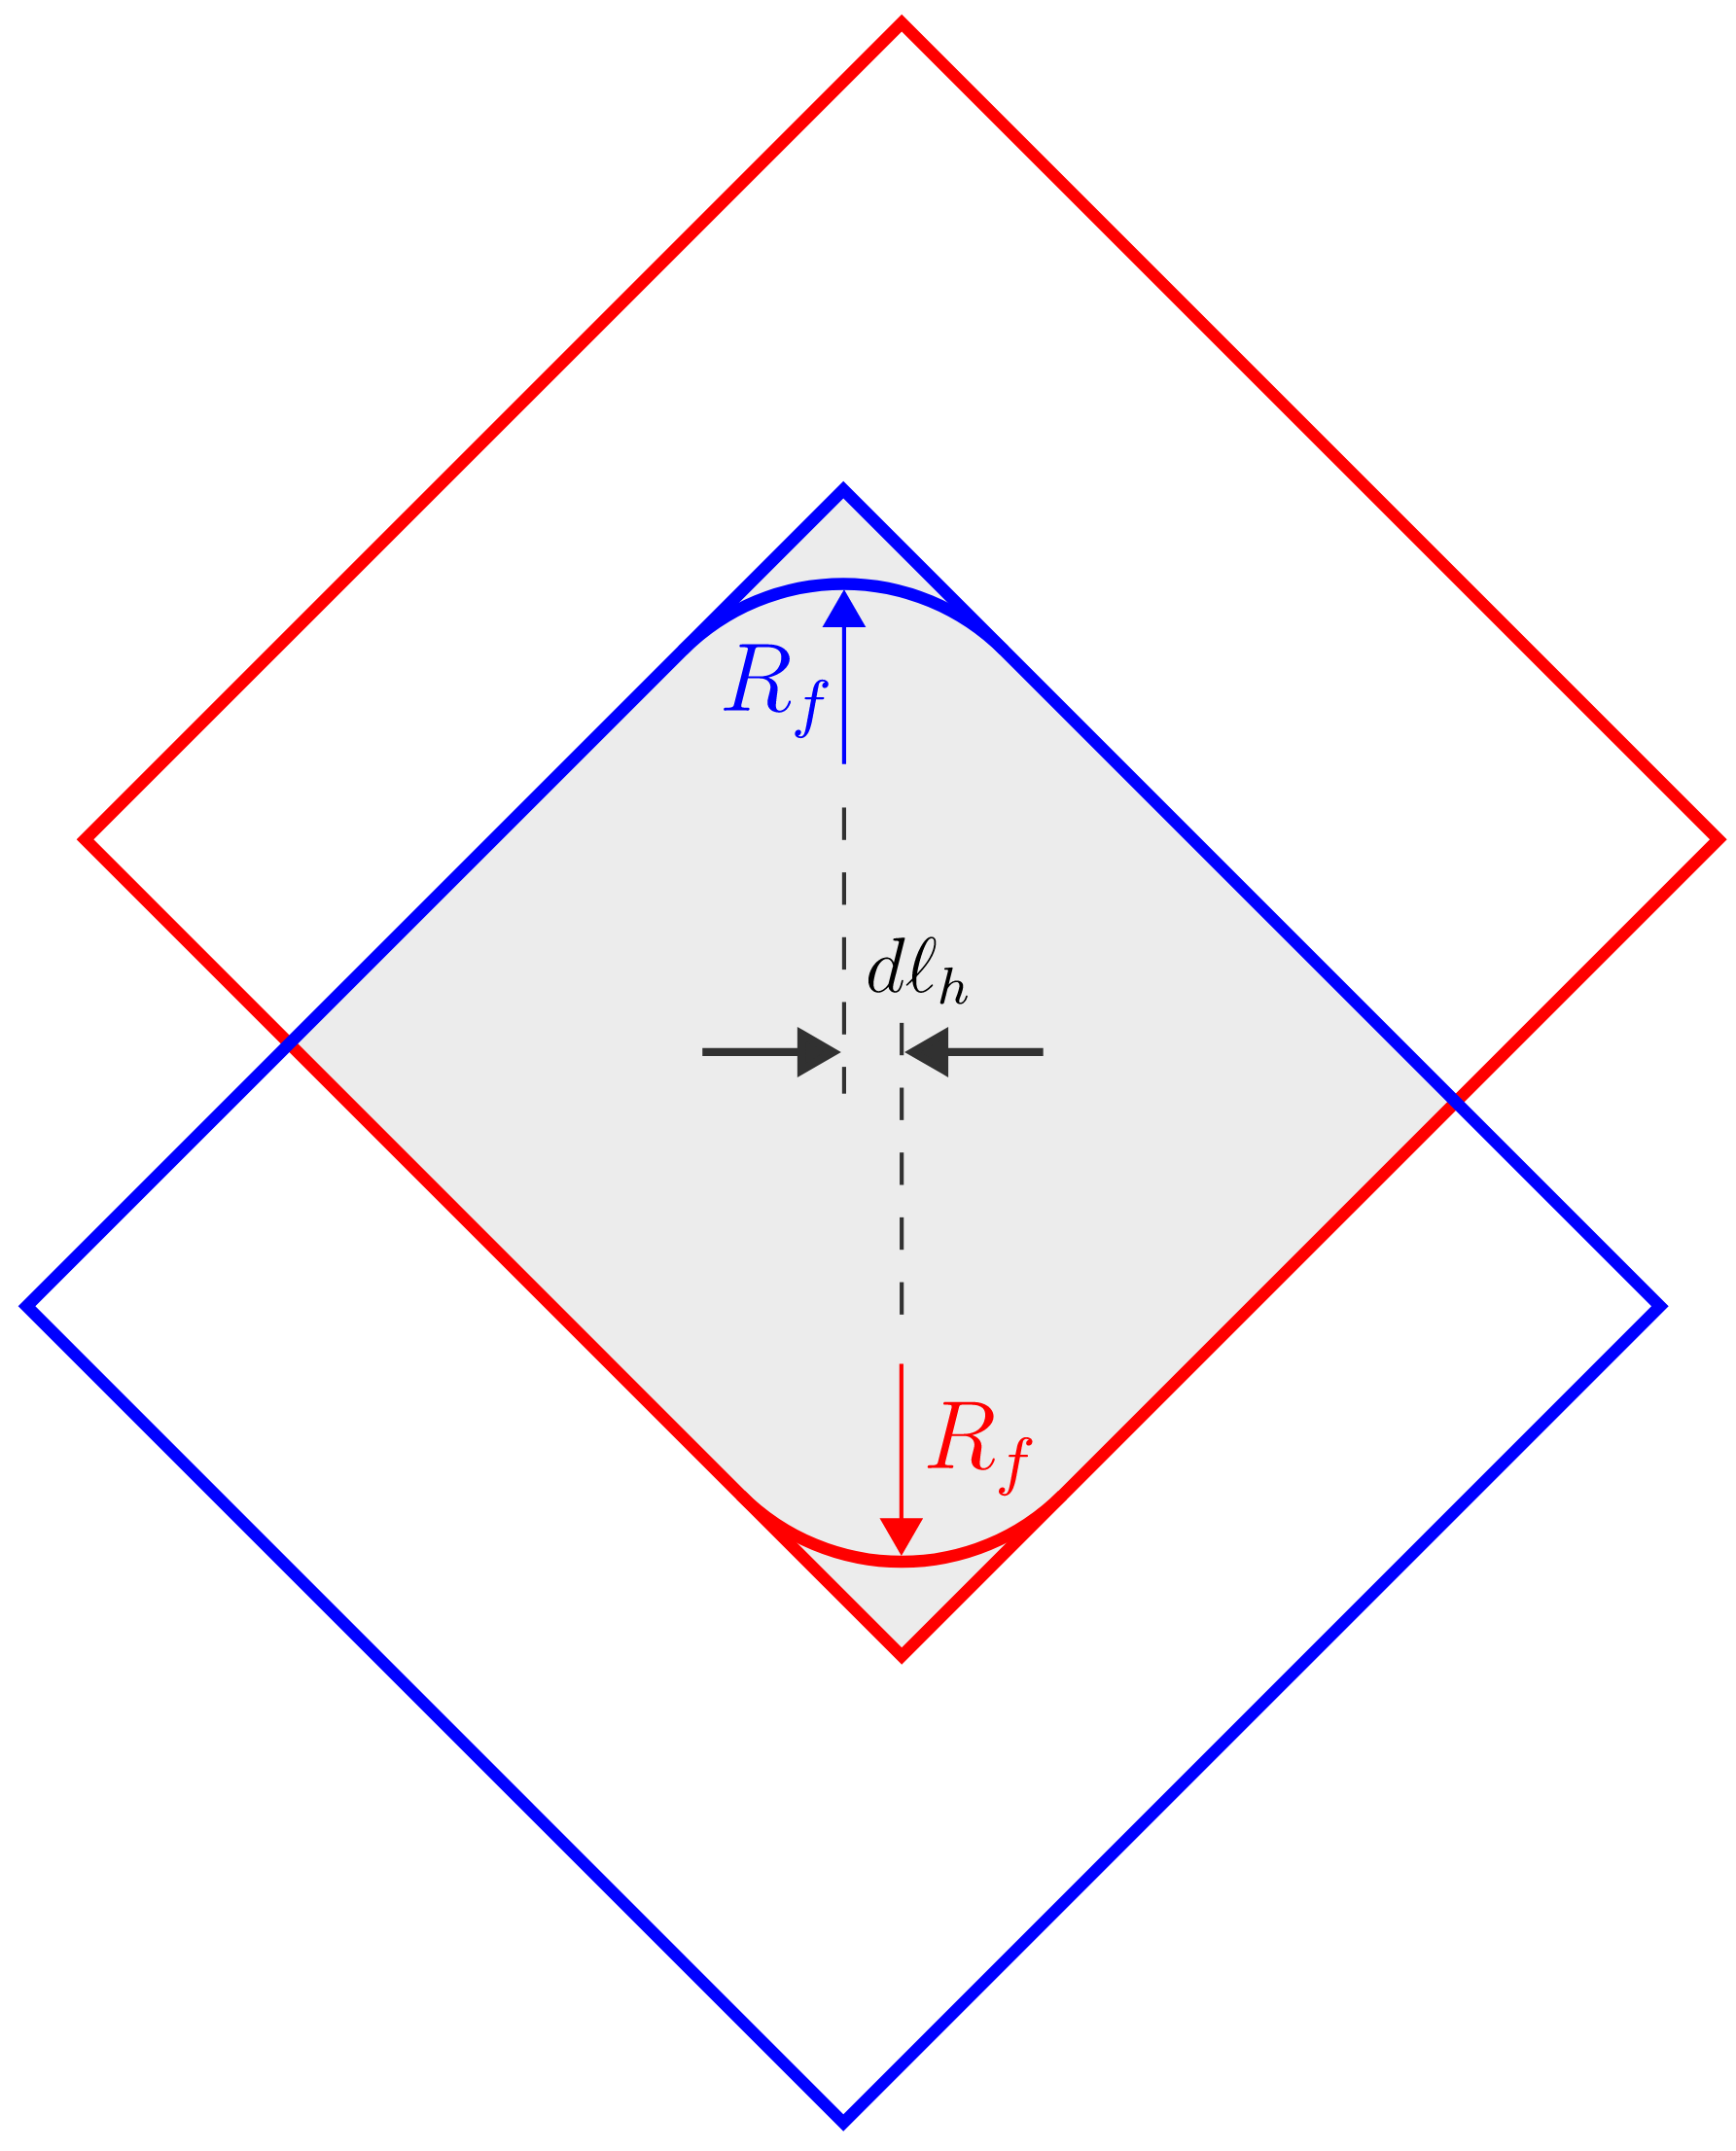
\includegraphics[width=.39\textwidth]{orif_error.png}
				\caption{Orifice error modes}
				\label{fig:orif_error}
			\end{wrapfigure}

			The two square holes that make the orifice will be machined with Sinker EDM. Two critical tolerances significantly influence the effective diameter of the orifice:
			the horizontal position of each hole and the fillet radii at the top and bottom vertices. The side vertices are made by the intersection of two straight cuts and can be assumed to be sharp.
			Figure~\ref{fig:orif_error} depicts these two error modes. Milco Wire EDM, Inc quoted the operation (attached in Appendix~\ref{app:datasheets}).
			They can achieve a minimum fillet radius $R_f = \SI{76.2}{\micro\meter}$ and horizontally position each orifice to a tolerance of \SI{12.7}{\micro\meter}.
			This horizontal error compounds if the leading orifice is machined too far left and the trailing orifice is machined too far right;
			the maximum error is twice this value. Thus, $d \ell_h = \SI{25.4}{\micro\meter}$.
			Vertical error can be more readily dealt with individually; thus, the noncompounding vertical error is defined as $d \ell_v = \SI{12.7}{\micro\meter}$.

		\subsection{Bellows Spring Reactions}
		\label{app:sat:error:bellows}

			As the actuator deflects and drives the valve stem downwards or pulls it upwards, the two bellows act as springs and provide a slight reaction force, possibly compressing or stretching the valve stem and actuator.
			Since each part behaves as a spring, the resulting coupled spring assembly is complex and requires a comprehensive force balance analysis to reconcile the final deflections.

		Other sources of error include unwanted thermal expansion of the housing and valve subcomponents and potential heat transfer from the hot internal gas.
		Each of these sources of error impacts the entire system. Since the behavior of each subsystem is coupled, the effect of these errors on the final output of the \device\ can only be analyzed by a rigorous static system analysis.
		As discussed in Section~\ref{subsec:DFMEA::tol}, the transfer function derived in the following section provides a tool for analysis of deterministic and stochastic error propagation across the full temperature range.

	\section{Transfer Function Derivation}
	\label{app:sat:TF}

		The required transfer function from Section~\ref{subsec:intro:specs:RR} describes the system under ideal conditions and cannot properly account for systematic errors.
		To fully analyze the expected performance of the \device, a new, comprehensive system Transfer Function must be derived that can be compared to the required output: 

		\begin{equation}
			\hat{G}_{sys} = A_1 (T-T_{ref}) + A_0 = (\Aone)(T-T_{ref}) + (\Azero)
			\label{eq:req_TF}
		\end{equation}

		This section presents a full derivation of this transfer function, represented in block-diagram form on the following page:
		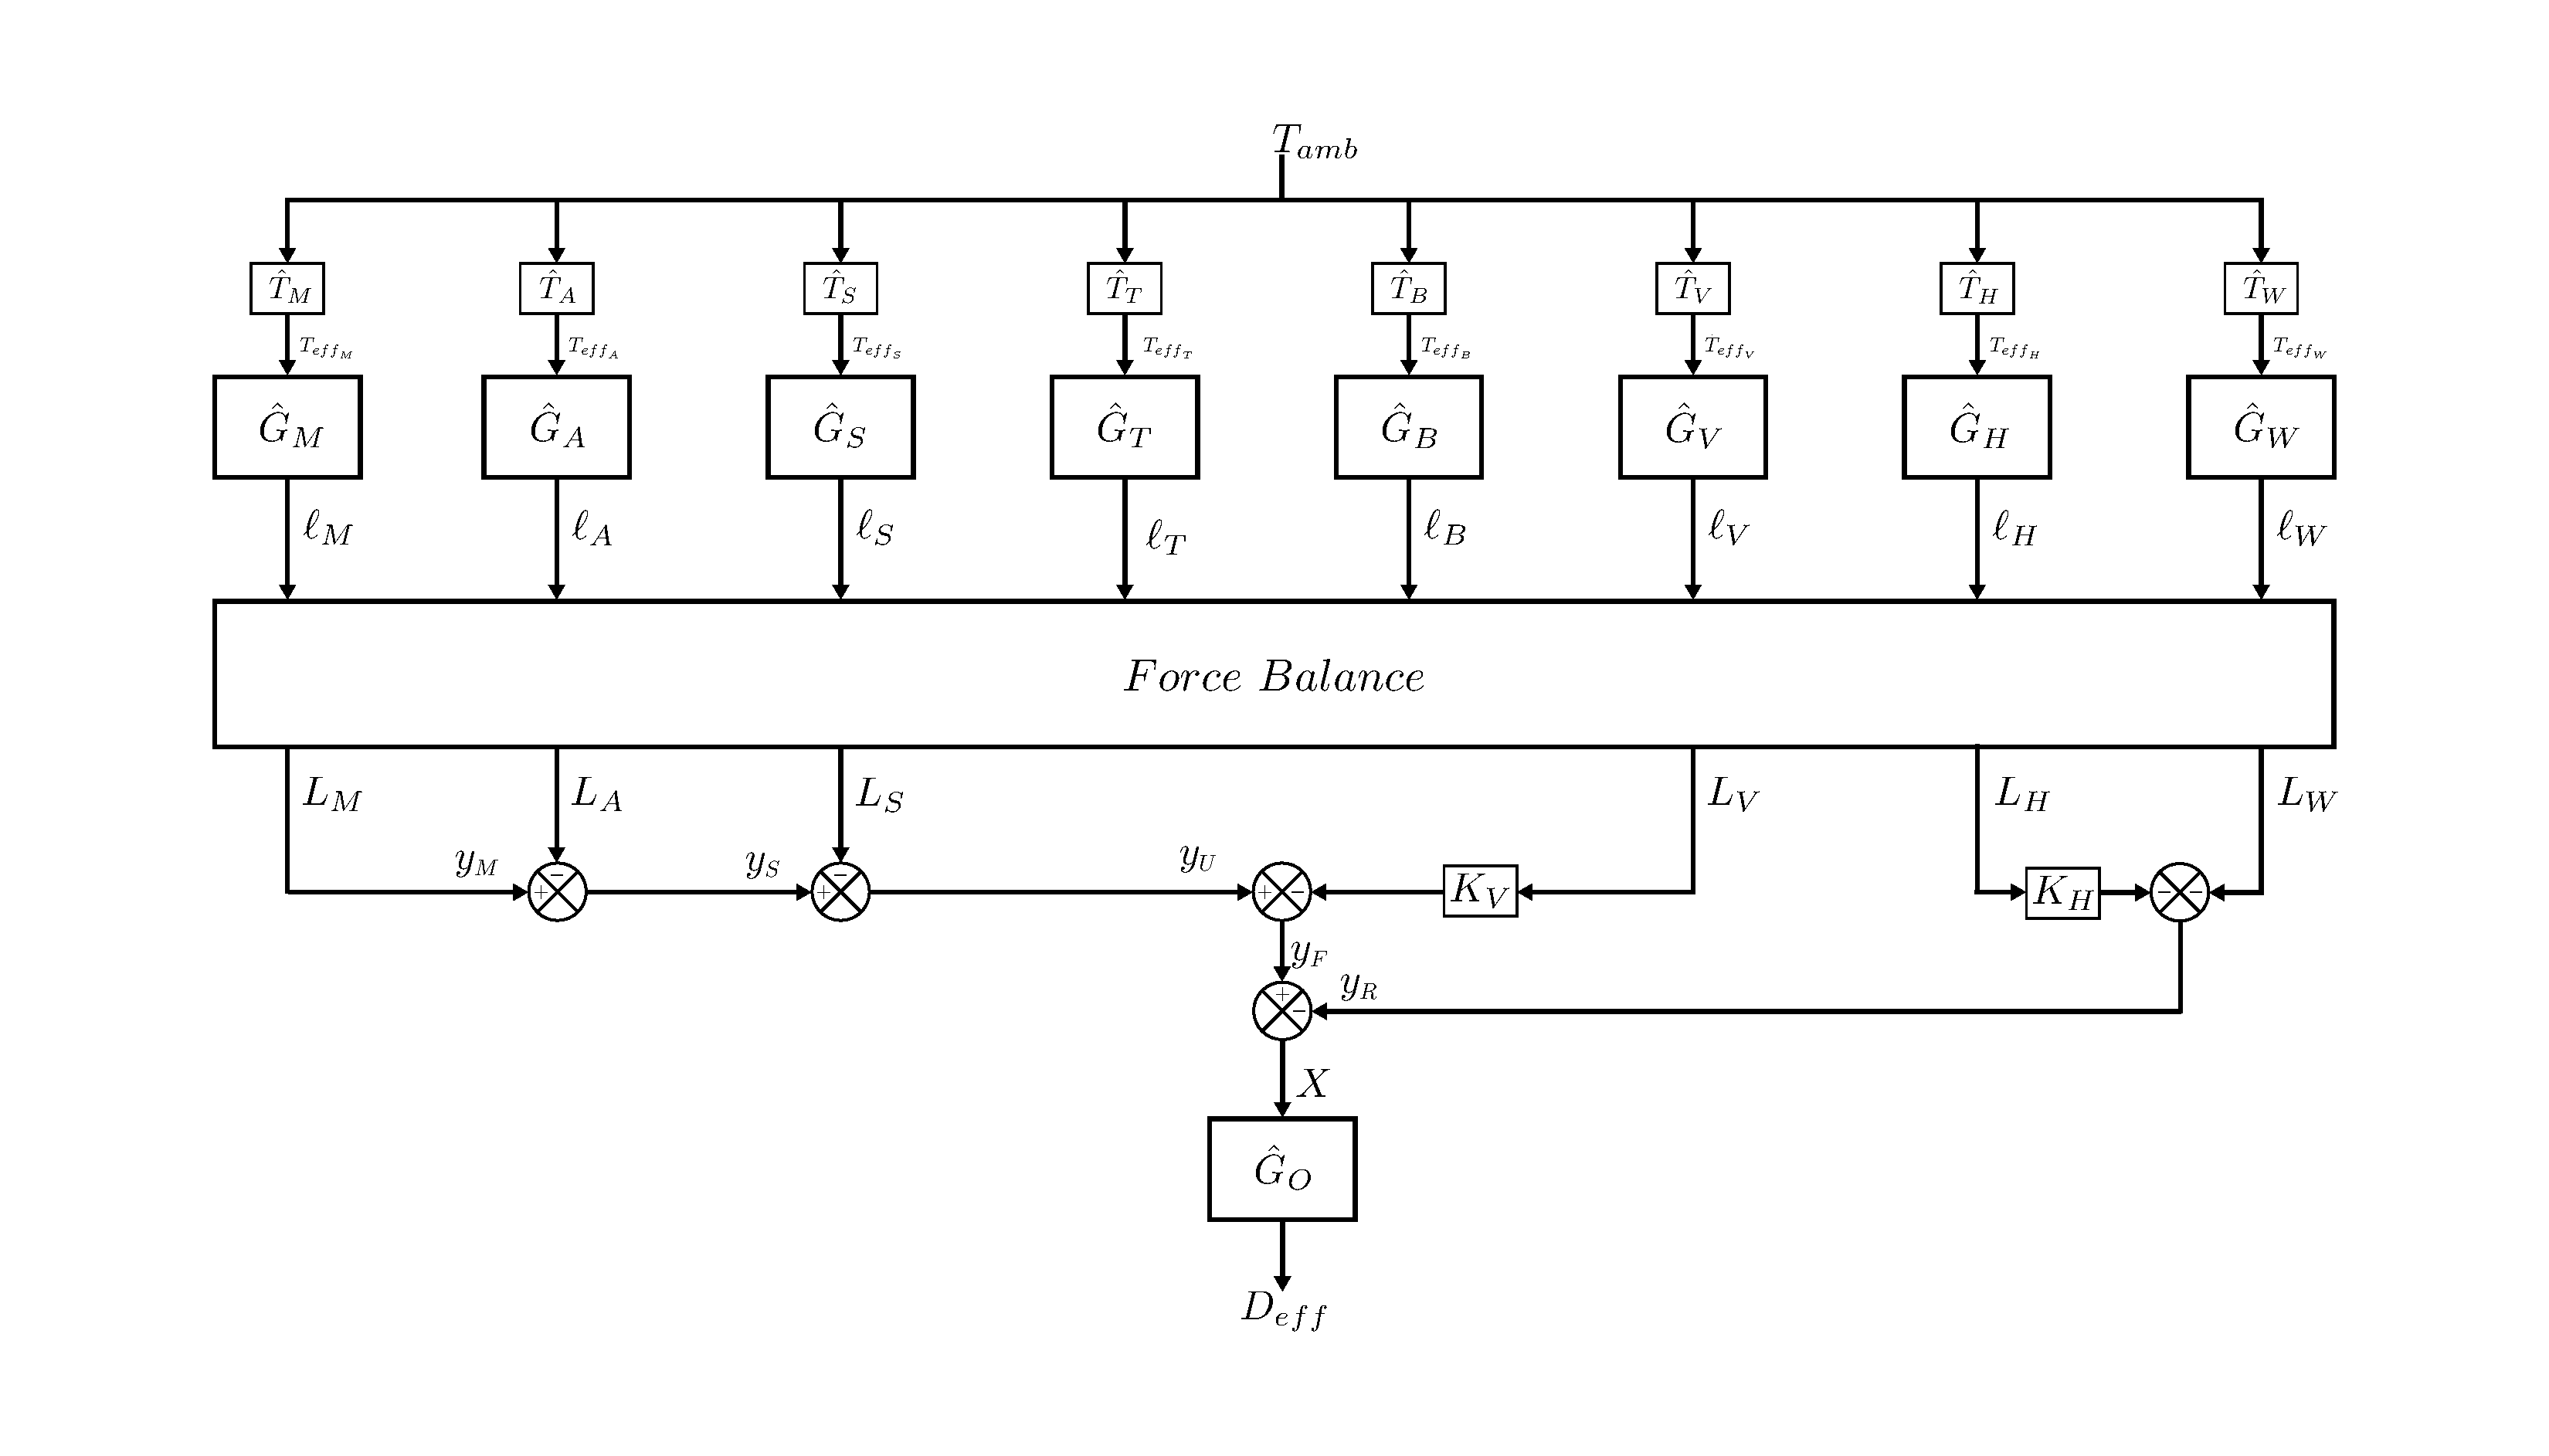
\includepdf[pages=1, fitpaper=true, landscape=true]{pdf/TF_import.pdf}

		The \device\ System Transfer Function comprises 21 smaller independent transfer functions whose respective output values are summed and equated in accordance with the physical behavior of the system.
		Its details will take a moment to unpack.

		First, notice the general structure: the transfer function receives $T_{ambient}$ and returns $D_{effective}$ as prescribed.
		The smaller, top $(\hat{T})$ row of sub-transfer functions adjusts $T_{amb}$ for each part in the assembly to account for heat transfer from the hot internal gas.
		The larger, second $(\hat{G})$ row represents the thermal expansion of each dimensionally critical component; each function takes the given adjusted temperature and outputs the thermally expanded length $\ell$ of its respective part.
		However, because the bellows apply a spring force against the actuation motion, these parts will deform slightly. A Force Balance processes these undeformed length values through a system of linear equations, yielding the final length $L$ of each component.
		These final values are summed to obtain the position $y$ of each of the two square holes. Taking the difference between these positions, we obtain the height $X$ of the square orifice, which is finally converted to $D_{effective}$ by the orifice transfer function $\hat{G}_O$.
		
		To understand the origin of the transfer function structure, we must decompose the functional structure of each component of the \device.
		Figure~\ref{fig:positional_block_diagram} illustrates the relative position of each component in simplified fashion.
		Each part's temperature adjustment function $\hat{T}$, thermal transfer function $\hat{G}$, undeformed length $\ell$, and final length $L$ is labeled with its respective subscript as shown in the figure:
		
		\begin{multicols}{2}
			\begin{itemize}
				\item Mount (M)
				\item Actuator (A)
				\item Upper valve stem (S)
				\item Upper ``top'' bellows (T)
				\item Lower ``bottom'' bellows (B)
				\item Valve orifice (V)
				\item Housing side walls (H)
				\item Housing top face or ``wall'' (W)
			\end{itemize}
		\end{multicols}

		The positional block diagram defines how each part is coupled to the others, enabling the force balance required to find the spring deflection of each flexible part.
		The labeled heights move as each part expands or contracts, yielding the final position of each orifice as the net sum of the stretched and compressed parts.
				
		\begin{figure}[H]
			\centering
			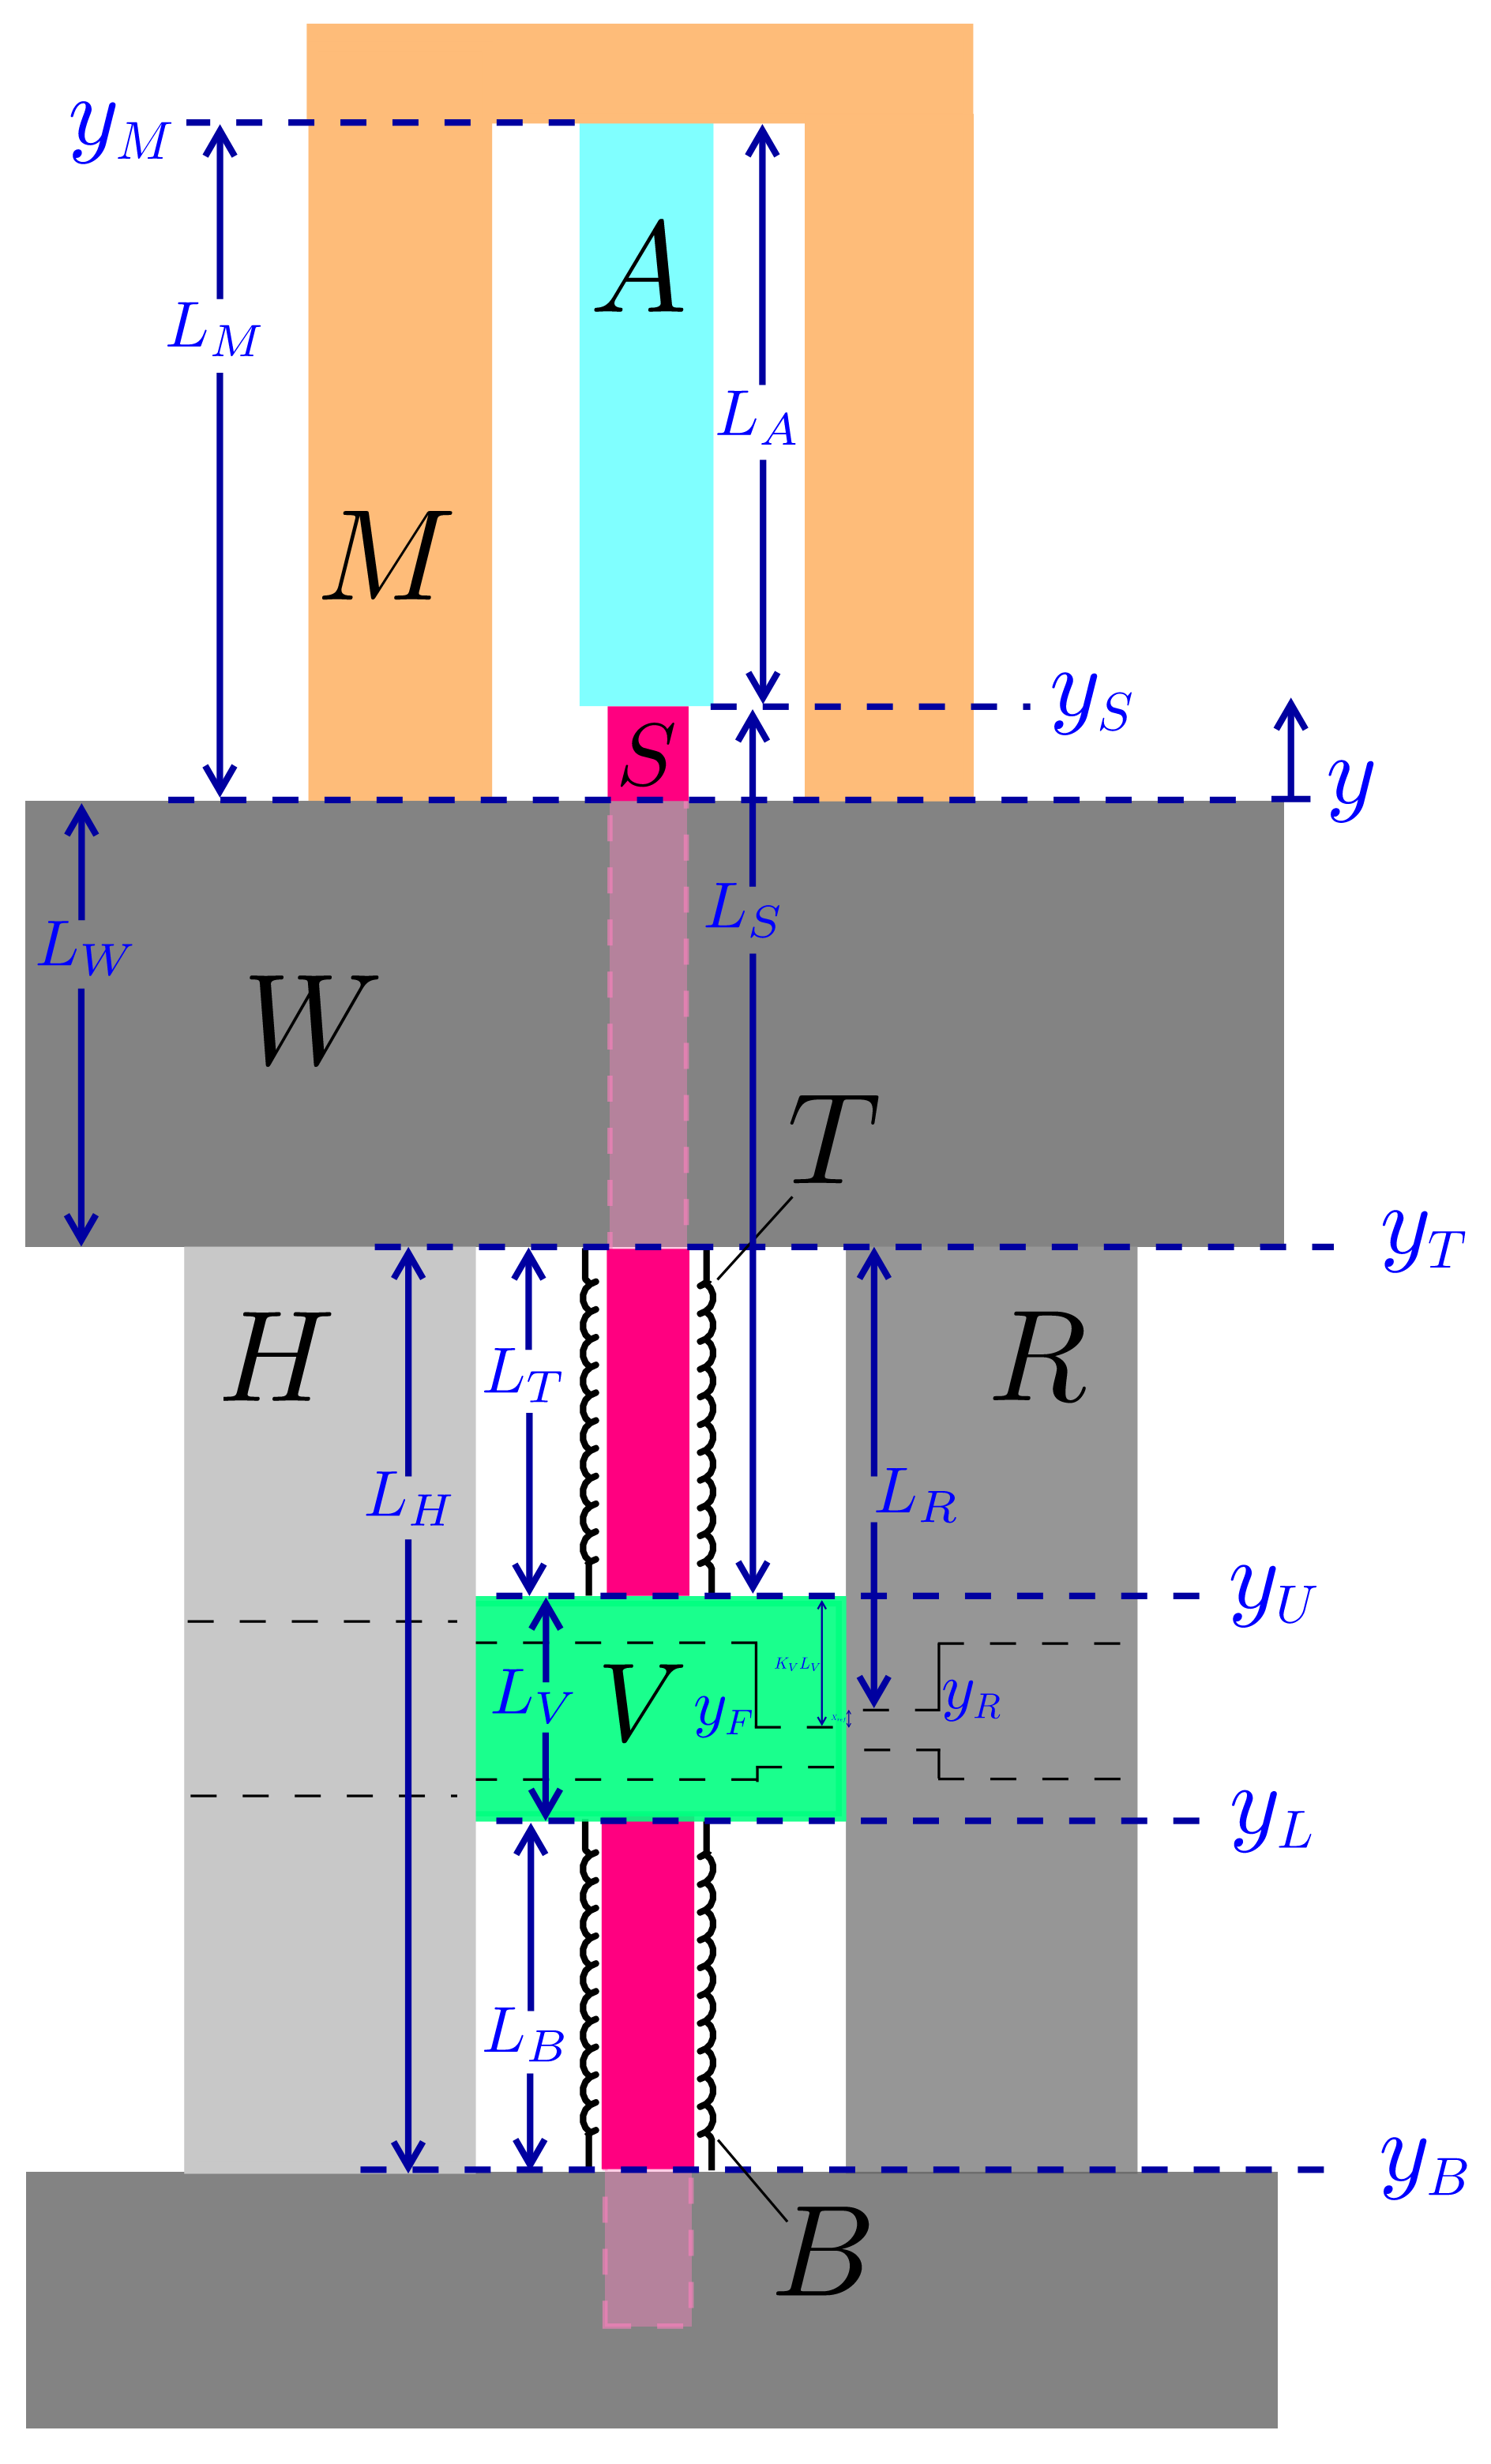
\includegraphics[height=.98\textheight, width=\textwidth, keepaspectratio]{positional_block_diagram.png}
			\caption{Positional block diagram}
			\label{fig:positional_block_diagram}
		\end{figure}
		
		
		\begin{multicols}{2}
			\begin{figure}[H]
				\centering
				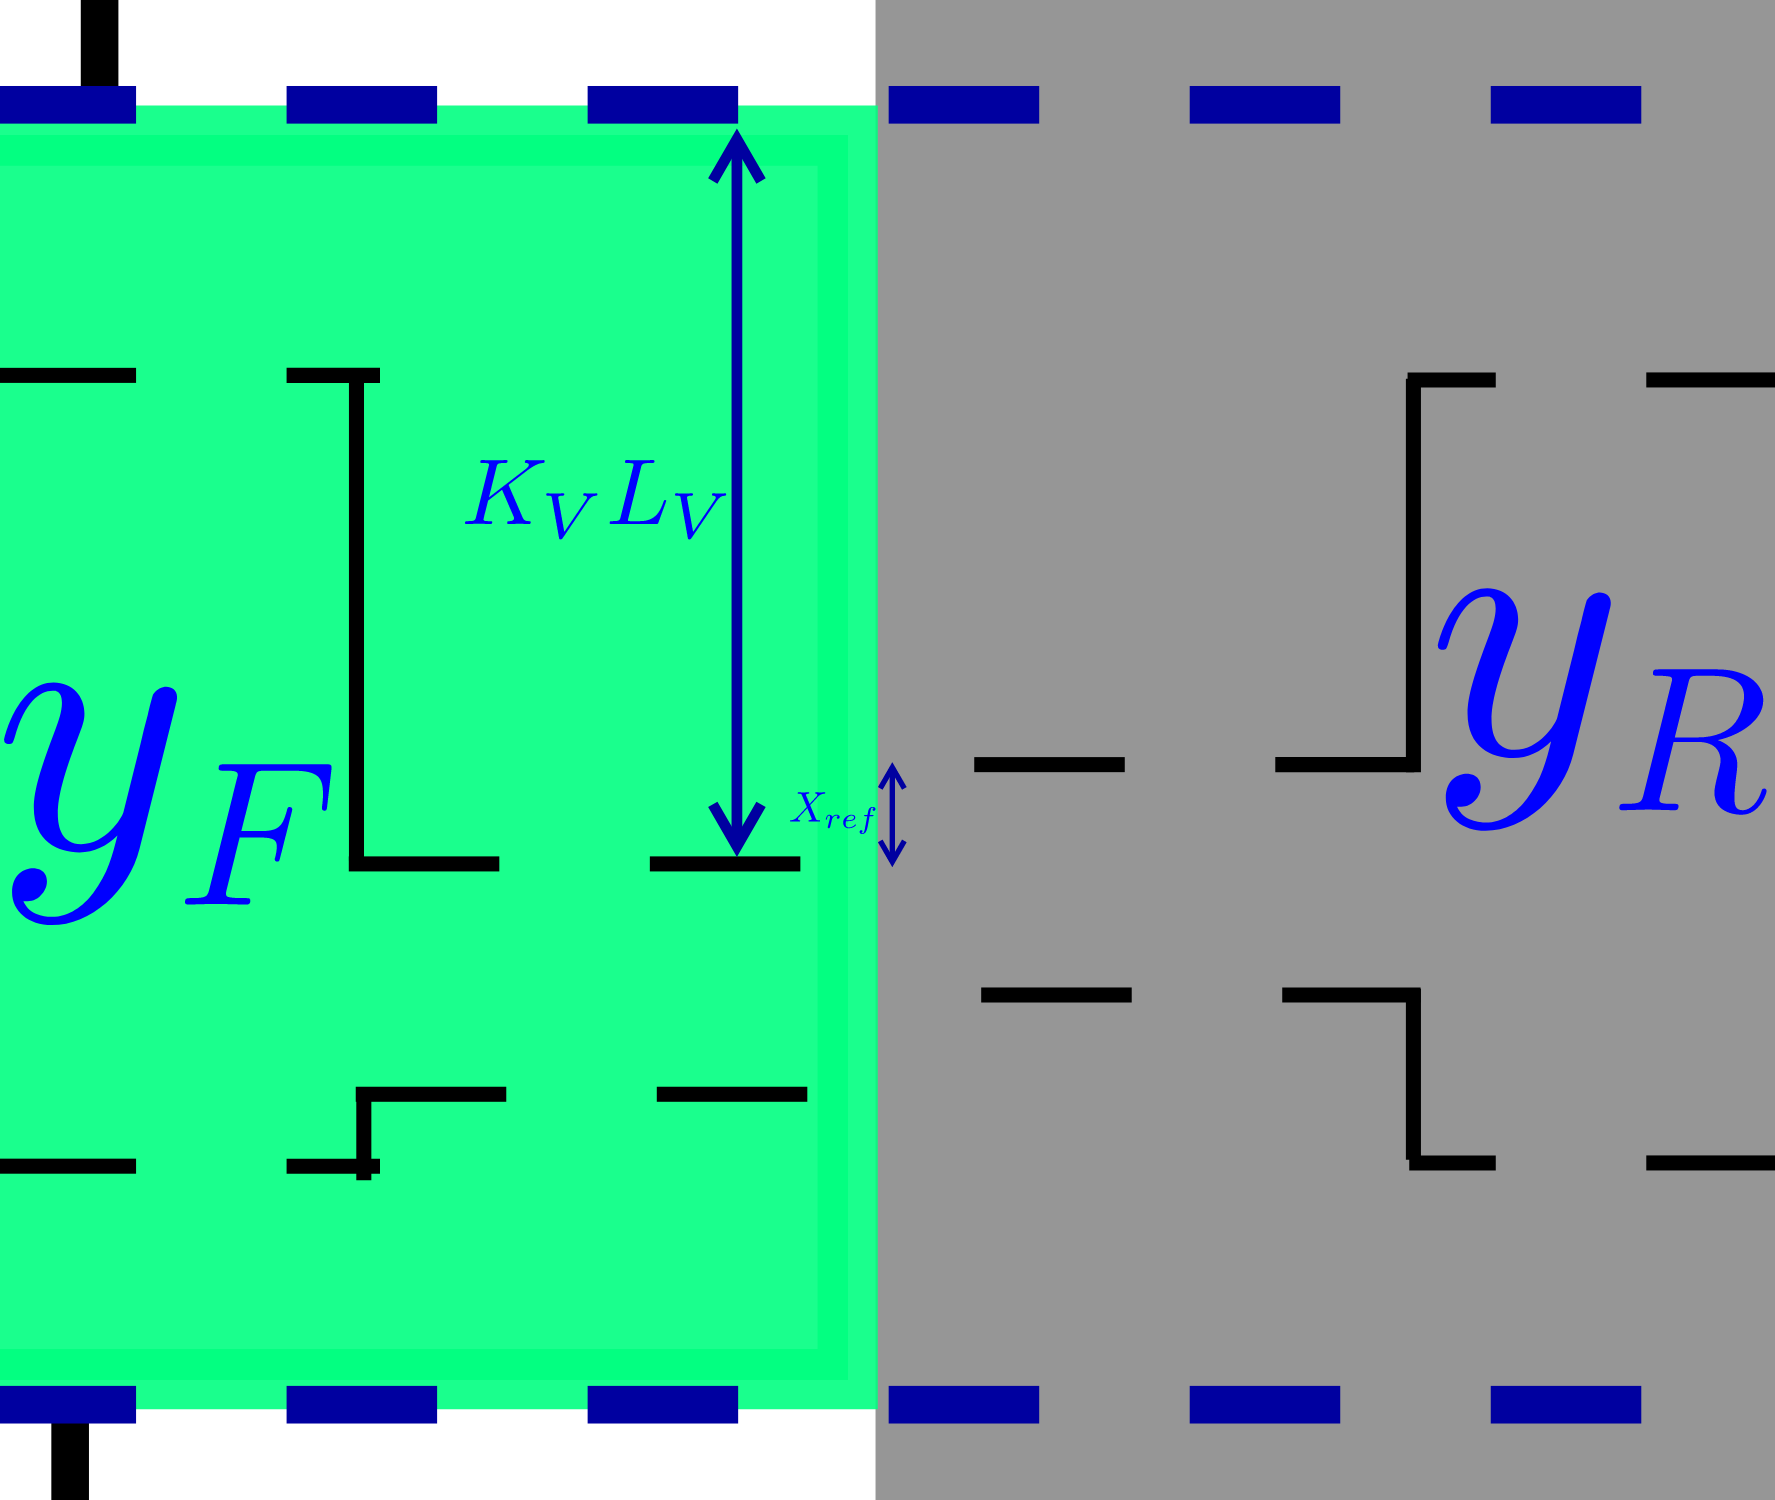
\includegraphics[width=.45\textwidth]{positional_block_diagram_zoom.png}
				\caption{Positional block diagram, detail view}
				\label{fig:positional_block_diagram_zoom}
			\end{figure}

			\begin{figure}[H]
				\centering
				\includegraphics[width=.45\textwidth]{Housing_split.png}
				\caption{Separation between Housing Wall (W) and Housing Body (H)}
				\label{fig:housing_split}
			\end{figure}

			\columnbreak
			
			Figure~\ref{fig:positional_block_diagram_zoom} shows a detail view of certain dimensions around the orifice that will be used later.
			As described in Chapter~\ref{chap:design}, the mount $(M)$ sits atop the housing.
			The actuator $(A)$ dangles from the upper interior surface of the housing center, which for our purposes is defined as the undersurface of the belleville washer.
			The upper valve stem $(S)$ hangs from the bottom of the actuator, passes through the housing wall, and suspends the valve orifice $(V)$, which slides freely against the two surfaces $H$ and $R$.
			Treating the three housing components as a single part, which is realistic because they are electron-beam welded at every seam, the housing ``wall'' $(W)$ is defined as the top \SI{10}{\milli\meter} of the whole housing assembly (parts V1, V2, and V3) as shown in Figure~\ref{fig:housing_split}.
			The housing body $(H)$ and ``rear'' $(R)$ share the lower portion shown in the figure; their expansion is coupled.
			These represent the side walls of the housing and behave identically; thus, their behavior is summed by the $H$ term in several calculations.
			The two bellows $(T \text{ and } B)$ span the distance between the valve orifice and the upper and lower housing walls (part V2).
			
			Figure~\ref{fig:positional_block_diagram} also defines several useful positions according to a vertical coordinate frame. The position variable $y$ originates (i.e. equals $0$) at the top surface of the housing, which is considered fixed, and increases vertically.
			Thus, $y_M$ is positive, whereas $y_T$ is negative.
		\end{multicols}

		\subsection{Heat Transfer}
		\label{app:sat:TF:dT}

			The very top row evaluates the final effective temperature of each part assuming a worst-case thermal gradient driven by a \SI{20}{\degreeCelsius} temperature difference between the internal gas
			and the ambient temperature. The temperature of every wetted part is set to the gas temperature. The actuator and mount temperatures are assumed to follow $T_{amb}$ exactly, but the tools for a more complex
			heat transfer analysis between the subsystems were developed in Chapter~\ref{chap:test}, providing a starting ground to determine the final steady-state temperature of the actuator.
			The results presented in this Appendix, however, do not properly reflect this heat transfer and simply show the output of the \device\ for gas that follows the ambient temperature.
		
		\subsection{Thermal Expansion}
		\label{app:sat:TF:G_therm}

			Let us forgo the top row of temperature-adjusting functions for now and assume we know the temperature of each part. A full thermal analysis will provide these values later in this report.
			Each of the nine sub-transfer functions along the second row computes the thermal expansion of each part shown in Figure~\ref{fig:positional_block_diagram}.
			Its value can be approximated as a first-order Taylor Expansion\cite{ref_Jensen}\cite{ref_Stewart} with very little error due to the linear behavior of thermal expansion. This yields

				\begin{equation}
					\ell_i = \hat{G}_{thermal} = \ell_0(1 + \frac{d \ell}{dT} \Delta T)
				\end{equation}

			where $\hat{G}_{thermal}$ outputs the expanded dimension $\ell_i$ of part $i$, $\ell_0$ is its machined dimension, and $\Delta T = (T_{amb} - T_{ref})$.
			According to the general principle of thermal expansion\cite[Eq.~4-4]{ref_Hibbeler}, $\frac{d \ell}{dT} = \alpha \ell_0$ where $\alpha$ is the material Coefficient of Thermal Expansion (CTE).
			Thus, the thermal-expansion transfer functions are defined as follows:

			\begin{align}
					\hat{G}_M &= \ell_{M_0} (1 + \alpha_{\mathrm{ALLV}} ( T_{{eff}_M} - T_{ref} ) ) &
					\hat{G}_B &= \ell_{B_0} (1 + \alpha_{Inc} ( T_{{eff}_B} - T_{ref} ) ) \label{eq:G_therm_1}\\
					\hat{G}_A &= \ell_{A_0} (1 + \alpha_{Al} ( T_{{eff}_A} - T_{ref} ) ) &
					\hat{G}_V &= \ell_{V_0} (1 + \alpha_{Inv} ( T_{{eff}_V} - T_{ref} ) ) \\
					\hat{G}_S &= \ell_{S_0} (1 + \alpha_{Inv} ( T_{{eff}_S} - T_{ref} ) ) &
					\hat{G}_H &= \ell_{H_0} (1 + \alpha_{Inv} ( T_{{eff}_H} - T_{ref} ) ) \\
					\hat{G}_T &= \ell_{T_0} (1 + \alpha_{Inc} ( T_{{eff}_T} - T_{ref} ) ) &
					\hat{G}_W &= \ell_{W_0} (1 + \alpha_{Inv} ( T_{{eff}_W} - T_{ref} ) ) \label{eq:G_therm_last}
			\end{align}

			where the material expansion coefficients and machined lengths are as follows.

			Material coefficients of thermal expansion:

			\begin{itemize}
				\item Aluminum (Al): \specActuatorCTE\cite[Table~9-22]{ref_NASA_specs_Al}
				\item Allvar (ALLV): \specMountCTE\cite{ref_AllvarAlloys}
				\item Invar 36 (Inv): \specInvarCTE\cite{ref_Carpenter_Inv}
				\item Inconel 718 (Inc): \specInconelCTE\cite{ref_SpecialMetals_Inc}
			\end{itemize}

			and the machined dimensions $\ell_{i_0}$ from Appendix~\ref{app:drawings}:

			\begin{itemize}
				\item $\ell_{M_0} = \SI{38.541}{\milli\meter} - \SI{0.55}{\milli\meter} = \SI{38.041}{\milli\meter}$\footnote{Top of the mount, for simplicity, is assumed to be the underside of the compressed belleville washer. Since this height is dependent on the use case, we will assume a \SI{0.05}{\milli\meter} compression.}
				\item $\ell_{A_0} = \SI{32.991}{\milli\meter}$
				\item $\ell_{S_0} = \SI{70.72}{\milli\meter} - \SI{32.86}{\milli\meter} = \SI{37.86}{\milli\meter}$
				\item $\ell_{T_0} = \SI{22.86}{\milli\meter}$
				\item $\ell_{B_0} = \ell_{T_0} = \SI{22.86}{\milli\meter}$
				\item $\ell_{V_0} = \SI{32.86}{\milli\meter} - \SI{27.86}{\milli\meter} = \SI{5}{\milli\meter}$
				\item $\ell_{H_0} = \SI{63.72}{\milli\meter}$
				\item $\ell_{W_0} = \SI{10}{\milli\meter}$
			\end{itemize}

			This yields nine undeformed lengths, helping us to define the positions of each part of the orifice.
			The CTE of aluminum is computed as a function of temperature as defined in Section~\ref{app:sat:error:CTE} to find the impact of this error on the final output.
			Dimensional errors are stochastically added or subtracted to each machined part length $\ell_0$. This process is discussed in more detail in Section~\ref{app:sat:TF:results}. 
			Before this can be calculated, however, the spring reaction of bellows must be reconciled.

		\subsection{Force Balance}
		\label{app:sat:TF:force_balance}

			Each component is undeformed at the machining and assembly temperature, $T_{ref}$. Thus, $L_i(T_{ref}) = \ell_i(T_{ref})$.
			As the temperature changes and the connected parts expand at different rates, the system behaves as a static coupled spring mechanism. The arrangement is shown in Figure~\ref{fig:springs}.

			\begin{figure}[H]
				\centering
				\begin{minipage}{.45\textwidth}
					\centering
					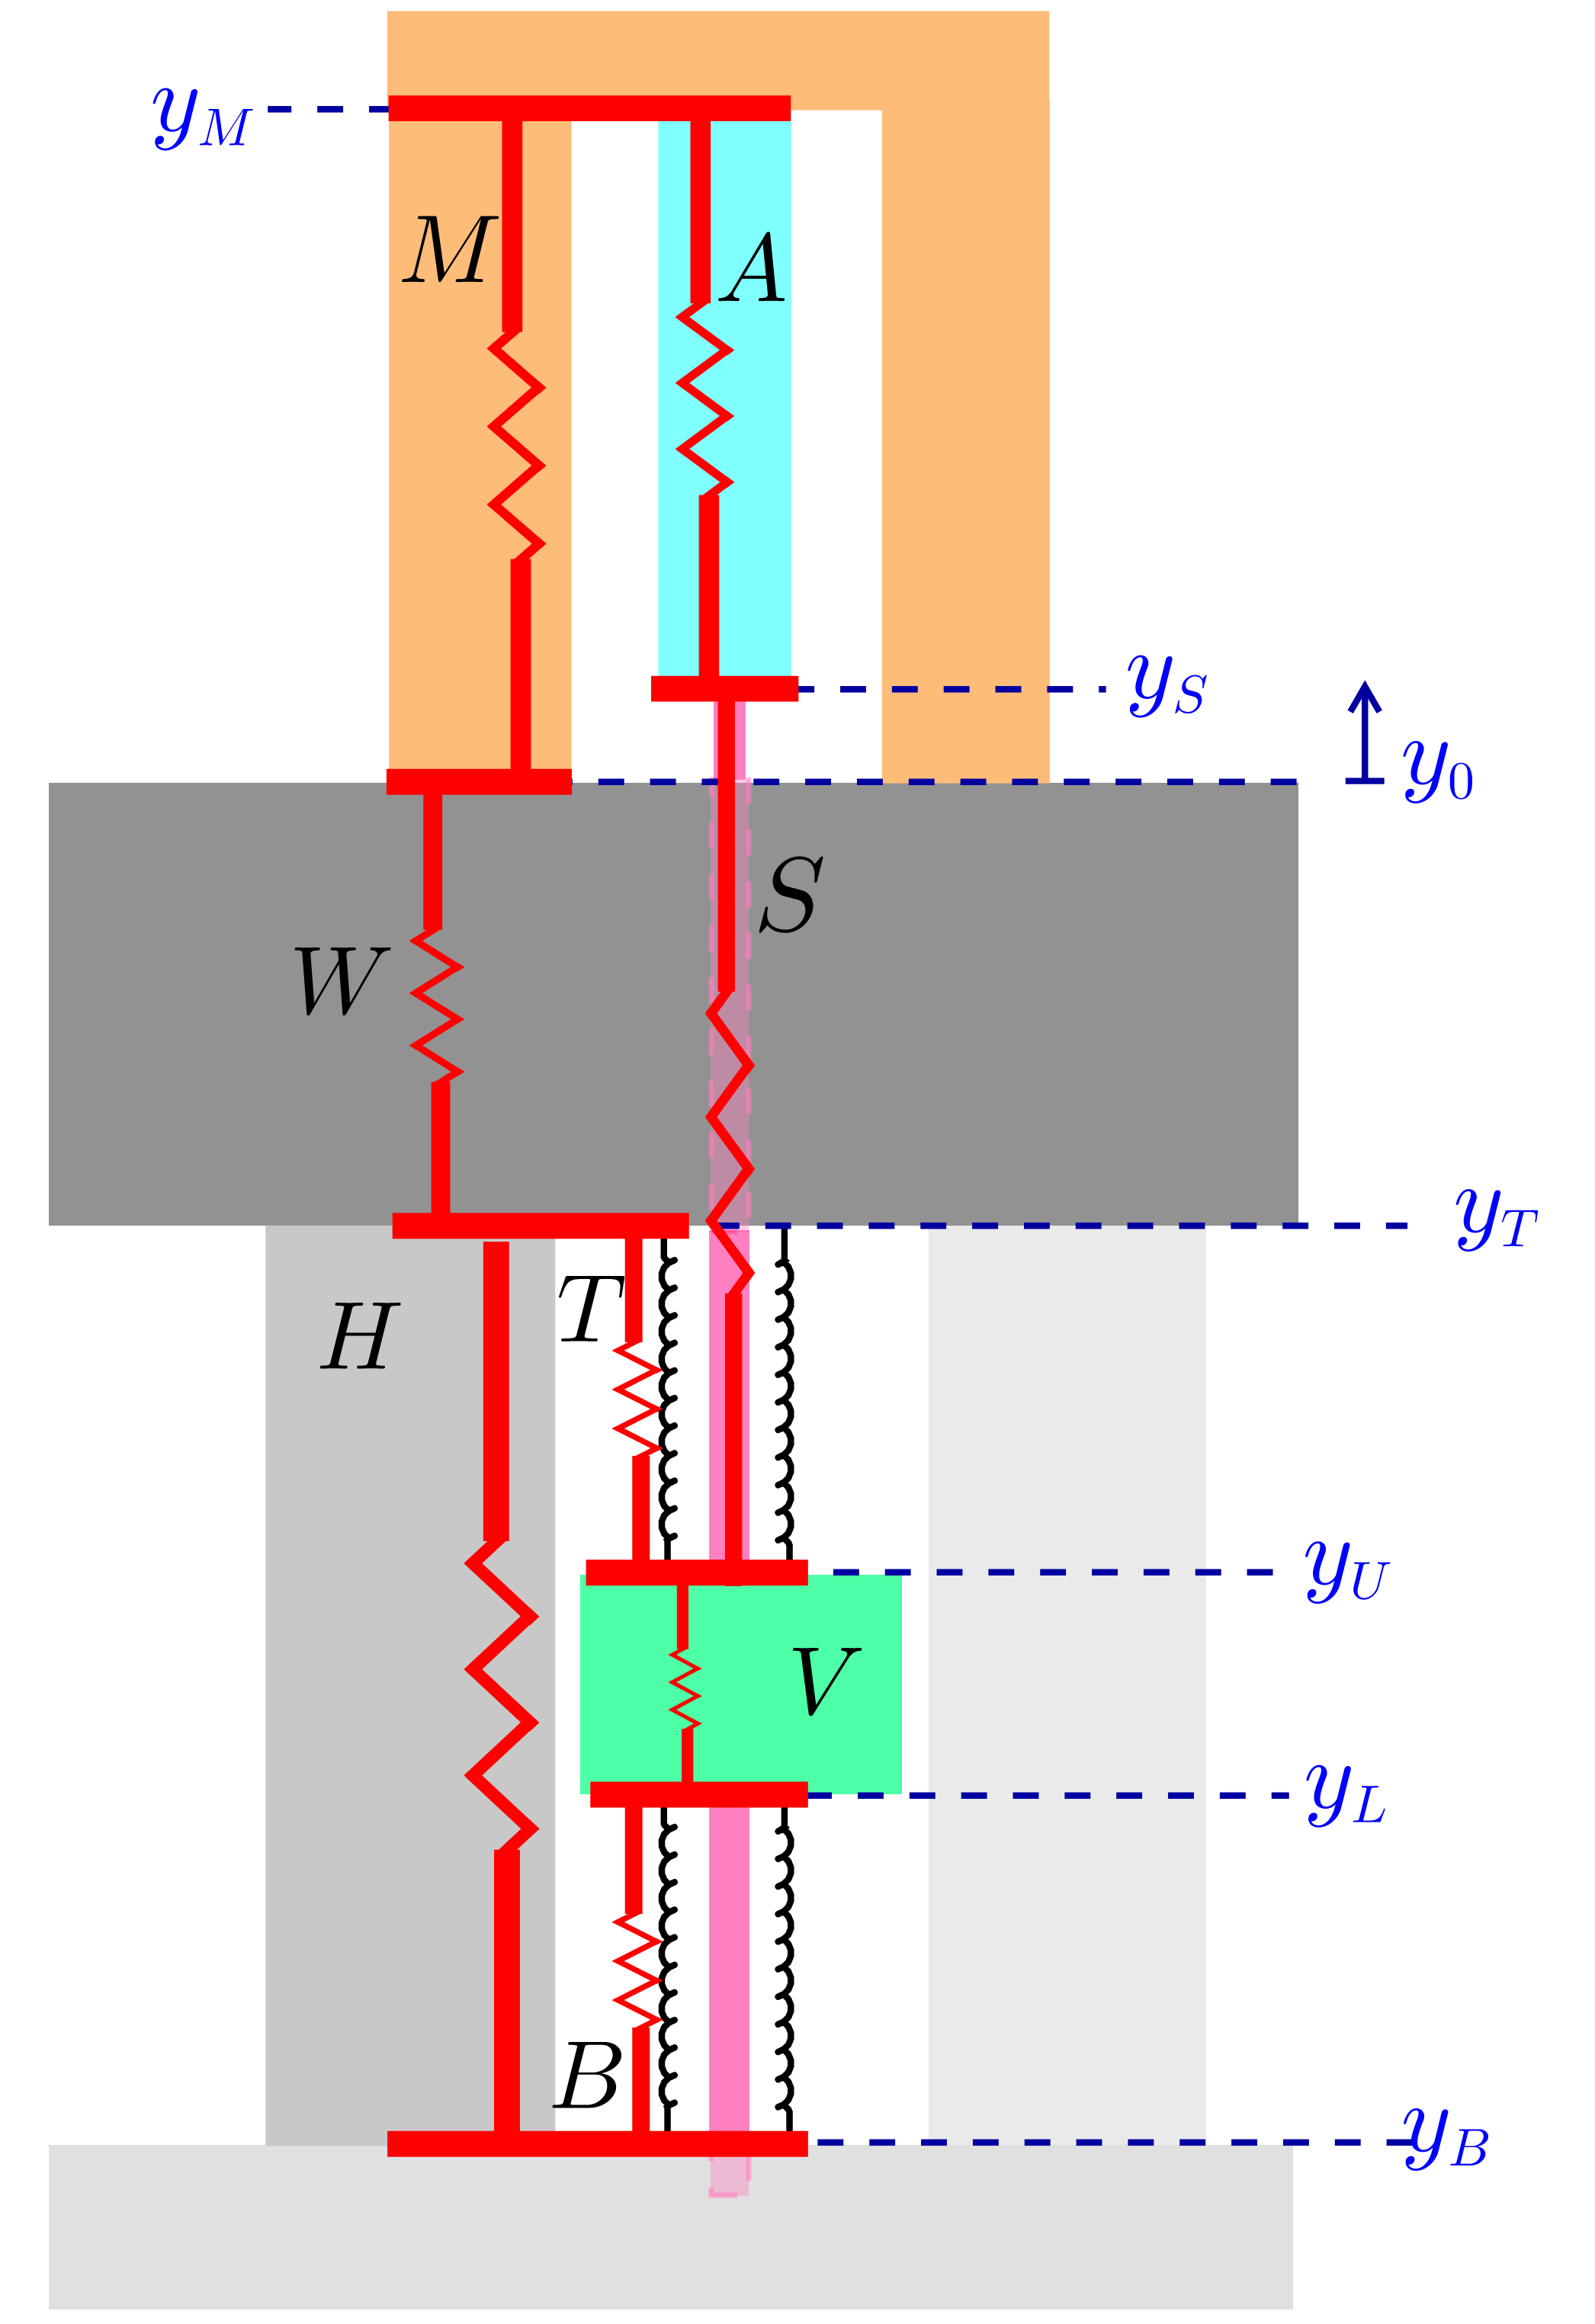
\includegraphics[height=.5\textheight]{springs.png}
					\subcaption{\device\ spring mechanism}
					\label{fig:springs_full}
				\end{minipage}
				\hfill
				\begin{minipage}{.45\textwidth}
					\centering
					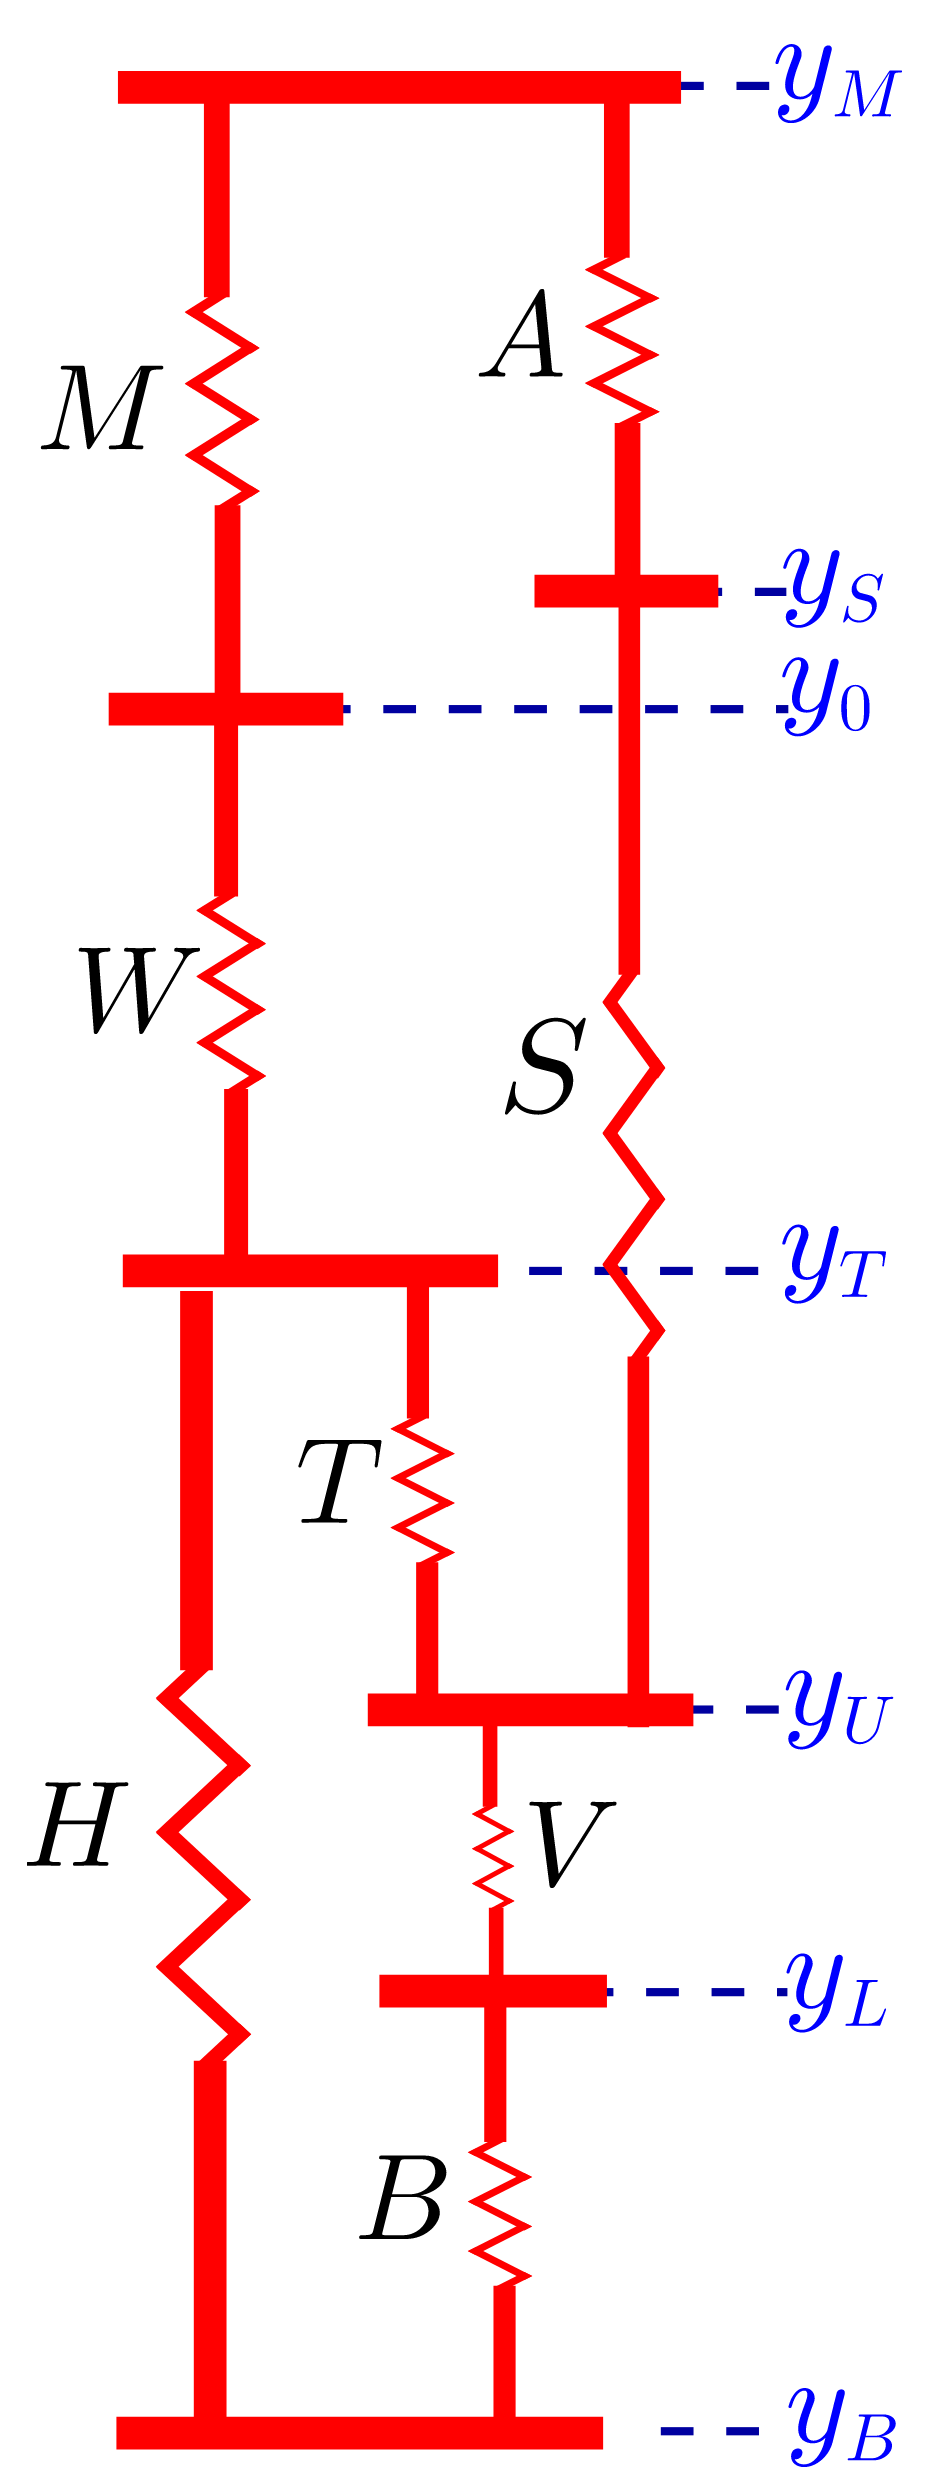
\includegraphics[height=.5\textheight]{springs_simp.png}
					\subcaption{\device\ spring mechanism, simplified}
					\label{fig:springs_simp}
				\end{minipage}
				\caption{Spring deflection}
				\label{fig:springs}
			\end{figure}


			Solution of the final lengths of these springs requires a system of equations, derived using static force analysis.
			We will use Figure~\ref{fig:springs_simp}, which accurately depicts the contact between parts, as our guide.
			The system contains seven nodes, labeled according to their subscripted position $y$, that we will use as the basis for our equations.
			For each nodal force balance, let us assume that the springs act along one degree of freedom (DOF), inducing no rotational moment.
			This is a safe assumption because, although the springs are depicted as spaced apart horizontally, they are concentric in the actual design.

			Equating upper and lower vertical forces at each node produces the following system of equations:

			\newcommand{\circlab}[1]{%
				\tikz[baseline=(char.base)]{
					\node[shape=circle, draw, inner sep=1pt,
						minimum size=1.5em] (char) {$#1$};
				}%
			}

			\newcommand{\ellipselab}[1]{%
				\tikz[baseline=(char.base)]{
					\node[shape=ellipse, draw, inner sep=1pt,
						minimum width=3.2em, minimum height=1.6em] (char) {$#1$};
				}%
			}

			\begin{equation}
				\left\{
				\begin{array}{ll}
					\circlab{y_M} & F_M + F_A = 0 \\[6pt]
					\circlab{y_S} & F_A = F_S \\[6pt]
					\circlab{y_0} & F_M = F_W \\[6pt]
					\circlab{y_T} & F_W = F_H + F_T \\[6pt]
					\circlab{y_U} & F_V = F_T + F_S \\[6pt]
					\circlab{y_L} & F_V = F_B \\[6pt]
					\circlab{y_B} & F_H + F_B = 0 \\
				\end{array}
				\right.
			\end{equation}

			This produces seven equations for eight unknown forces $(F_M, F_A, F_S, F_T, F_B, F_V, F_H, \text{ and } F_W)$.
			One might observe that this system remains indeterminate without one additional equation\footnote{It is well-established in the field of Linear Algebra that a system of linear equations with more equations than unknowns is linearly dependent (one or more equations is redundant) or self-contradictory, while that with more unknowns than equations is incomplete. A determinate system of equations requires exactly as many linearly independent equations as unknowns\cite{ref_Anton}.}.
			In fact, this system is linearly dependent and, when rearranged, contains a pair of redundant equations.

			From equations $y_M$, $y_S$, and $y_0$:

			\begin{align*}
				F_M &= F_W \\
				F_A &= -F_M = -F_W \\
				F_S &= F_A = -F_W
			\end{align*}

			From equations $y_L$ and $y_B$:

			\begin{align*}
				F_B &= F_V \\
				F_H &= -F_B = -F_V
			\end{align*}

			Substituting these into equations $y_T$ and $y_U$:

			\begin{align*}
				F_W &= -F_V + F_T \\
				F_V &= F_T - F_W
			\end{align*}

			These equations are linearly dependent and therefore redundant; one can easily rearrange one to equal the other. Thus, we will strike equation~$y_U$, leaving us six equations and eight unknowns.

			By Hooke's Law\cite{ref_Young_Freedman}, $F = k \Delta X$, we can substitute their forces for known spring constants, known undeformed lengths (as output by the thermal transfer functions), and unknown final lengths.
			The final two equations are supplied by two parallel length equalities: between $y_M$ and $y_U$ and between $y_T$ and $y_B$.

			\begin{equation}
				\left\{
				\begin{array}{ll}
					\circlab{y_M} & k_M(L_M - \ell_M) + k_A(L_A - \ell_A) = 0 \\[6pt]
					\circlab{y_S} & k_A(L_A - \ell_A) = k_S(L_S - \ell_S) \\[6pt]
					\circlab{y_0} & k_M(L_M - \ell_M) = k_W(L_W - \ell_W) \\[6pt]
					\circlab{y_T} & k_W(L_W - \ell_W) = k_H(L_H - \ell_H) + k_T(L_T - \ell_T) \\[6pt]
					\circlab{y_L} & k_V(L_V - \ell_V) = k_B(L_B - \ell_B) \\[6pt]
					\circlab{y_B} & k_H(L_H - \ell_H) + k_B(L_B - \ell_B) = 0 \\[6pt]
					\ellipselab{y_M \rightarrow y_U} & L_M + L_W + L_T = L_A + L_S \\[6pt]
					\ellipselab{y_T \rightarrow y_B} & L_H = L_T + L_V + L_B
				\end{array}
				\right.
			\end{equation}

			Now we have a system of eight equations with eight unknowns. These can be analytically solved using a matrix calculator by rearranging as follows:

			\begin{equation}
				\left\{
				\begin{array}{l}
					k_M L_M + k_A L_A = k_M \ell_M + k_A \ell_A \\[6pt]
					k_A L_A - k_S L_S = k_A \ell_A - k_S \ell_S \\[6pt]
					k_M L_M - k_W L_W = k_M \ell_M - k_W \ell_W \\[6pt]
					k_W L_W - k_T L_T - k_H L_H = k_W \ell_W - k_T \ell_T - k_H \ell_H \\[6pt]
					k_V L_V - k_B L_B = k_V \ell_V - k_B \ell_B \\[6pt]
					k_B L_B + k_H L_H = k_B \ell_B + k_H \ell_H \\[6pt]
					L_M - L_A - L_S + L_T + L_W = 0 \\[6pt]
					L_T + L_B + L_V - L_H = 0
				\end{array}
				\right.
			\end{equation}

			\begin{equation}
				\begin{bmatrix}
					k_M & k_A  & 0    & 0     & 0     & 0     & 0     & 0     \\
					0   & k_A  & -k_S & 0     & 0     & 0     & 0     & 0     \\
					k_M & 0    & 0    & 0     & 0     & 0     & 0     & -k_W  \\
					0   & 0    & 0    & -k_T  & 0     & 0     & -k_H  & k_W   \\
					0   & 0    & 0    & 0     & -k_B  & k_V   & 0     & 0     \\
					0   & 0    & 0    & 0     & k_B   & 0     & k_H   & 0     \\
					1   & -1   & -1   & 1     & 0     & 0     & 0     & 1    \\
					0   & 0    & 0    & 1     & 1     & 1     & -1    & 0
				\end{bmatrix}
				\begin{bmatrix}
					L_M \\ L_A \\ L_S \\ L_T \\ L_B \\ L_V \\ L_H \\ L_W
				\end{bmatrix}
				=
				\begin{bmatrix}
					k_M \ell_M + k_A \ell_A \\
					k_A \ell_A - k_S \ell_S \\
					k_M \ell_M - k_W \ell_W \\
					k_W \ell_W - k_T \ell_T - k_H \ell_H \\
					k_V \ell_V - k_B \ell_B \\
					k_H \ell_H + k_B \ell_B \\
					0 \\
					0
				\end{bmatrix}
				\label{eq:app_matrix}
			\end{equation}

			Each undeformed length $\ell$ is provided by the thermal transfer functions. With the exception of the two bellows, whose spring constants are given, each spring constant $k$ is calculated by material properties and part geometry\cite[Eq.~4-2]{ref_Hibbeler}:
			
			\begin{equation}
				k = \frac{EA}{\ell}
				\label{eq:k}
			\end{equation}
			
			where $E$ is the elastic modulus, $A$ is the cross-sectional area, and $\ell$ is defined as before.
			Each piece, though nearly rigid, is slightly flexible and can be modeled as a spring under axial load.
			Equation~\eqref{eq:k} provides the equivalent spring constant for each part, calculated below:
			
			\subsubsection{Mount}
			\label{app:sat:TF:force_balance:M}

				$E_M = E_{\text{ALLVAR}} = \specEALLV$\cite{ref_AllvarAlloys}
				
				$A_M = \frac{\pi}{4} (OD^2 - ID^2) = \frac{\pi}{4} [(\SI{25}{\milli\meter})^2 - (\SI{18}{\milli\meter})^2] = \SI{236.4}{\milli\meter\squared}$

			\subsubsection{Actuator}
			\label{app:sat:TF:force_balance:A}

				$E_A = E_{\text{Aluminum}} = \specEAl$\cite[p.~39]{ref_NASA_specs_Al}

				$A_A = \frac{\pi}{4} D^2 = \frac{\pi}{4} (\SI{18}{\milli\meter})^2 = \SI{254.5}{\milli\meter\squared}$

			\subsubsection{Valve Stem}
			\label{app:sat:TF:force_balance:S}

				$E_S = E_{\text{Invar}} = \specEInv $\cite{ref_Carpenter_Inv}

				$A_S = \frac{\pi}{4} D^2 = \frac{\pi}{4} (\SI{3.353}{\milli\meter})^2 = \SI{2.6}{\milli\meter\squared}$
				
			\subsubsection{Bellows}
			\label{app:sat:TF:force_balance:TB}

				$k_T = k_B = \specBellowsK $\cite{ref_miniflex_design}

			\subsubsection{Valve Orifice}    
			\label{app:sat:TF:force_balance:V}
			
			$E_V = E_{\text{Invar}} = \specEInv $
			
			$A_V = LW = (\SI{7}{\milli\meter}) (\SI{7}{\milli\meter}) = \SI{49}{\milli\meter\squared}$
			
			\subsubsection{Housing}    
			\label{app:sat:TF:force_balance:H}

				$E_H = E_{\text{Invar}} = \specEInv $

				$A_H = LW = (\SI{72}{\milli\meter}) (\SI{40}{\milli\meter}) = \SI{2880}{\milli\meter\squared}$

			\subsubsection{Top wall}
			\label{app:sat:TF:force_balance:W}

				$E_W = E_{\text{Invar}} = \specEInv $

				$A_W = A_H = \SI{2880}{\milli\meter\squared}$

			These spring constants are input into equation~\eqref{eq:app_matrix} to solve for the deformed length of each part.

		\subsection{Position calculations}
		\label{app:sat:TF:pos}

			Finally, we can use these lengths to calculate the values $y_F$ and $y_R$ of the two orifice components shown in Figure~\ref{fig:positional_block_diagram_zoom}.
			Using the scheme depicted in Figure~\ref{fig:positional_block_diagram}, these are as follows:

				\begin{align}
					y_F &= L_M - L_A - L_S - K_V L_V \label{eq:yF}\\
					y_R &= - K_H (2 L_W + L_H) \label{eq:yR}
				\end{align}

			To reach the upper corner of the leading orifice, which is cut into the Valve Orifice part, from the top surface of the housing (our reference location, where $y=0$),
			one must travel up the mount, down the actuator, down the valve stem, and partway down the valve orifice.
			To reach the lower corner of the trailing orifice, which is cut into the Housing Outlet, from the same reference position,
			one must travel straight down the housing wall.
			Because $L_V$ and $L_H$ represent the total height of the valve orifice and housing outlet, a multiplier is required to find the position of each square cut.
			The scaling constant $K_V$ defines the position of the upper vertex of the leading orifice, and $K_H$ the lower vertex of the trailing orifice, determined by its machined dimensions as shown in Figure~\ref{fig:K_pos}.

			\begin{wrapfigure}{l}{0.5\textwidth}
				\centering
				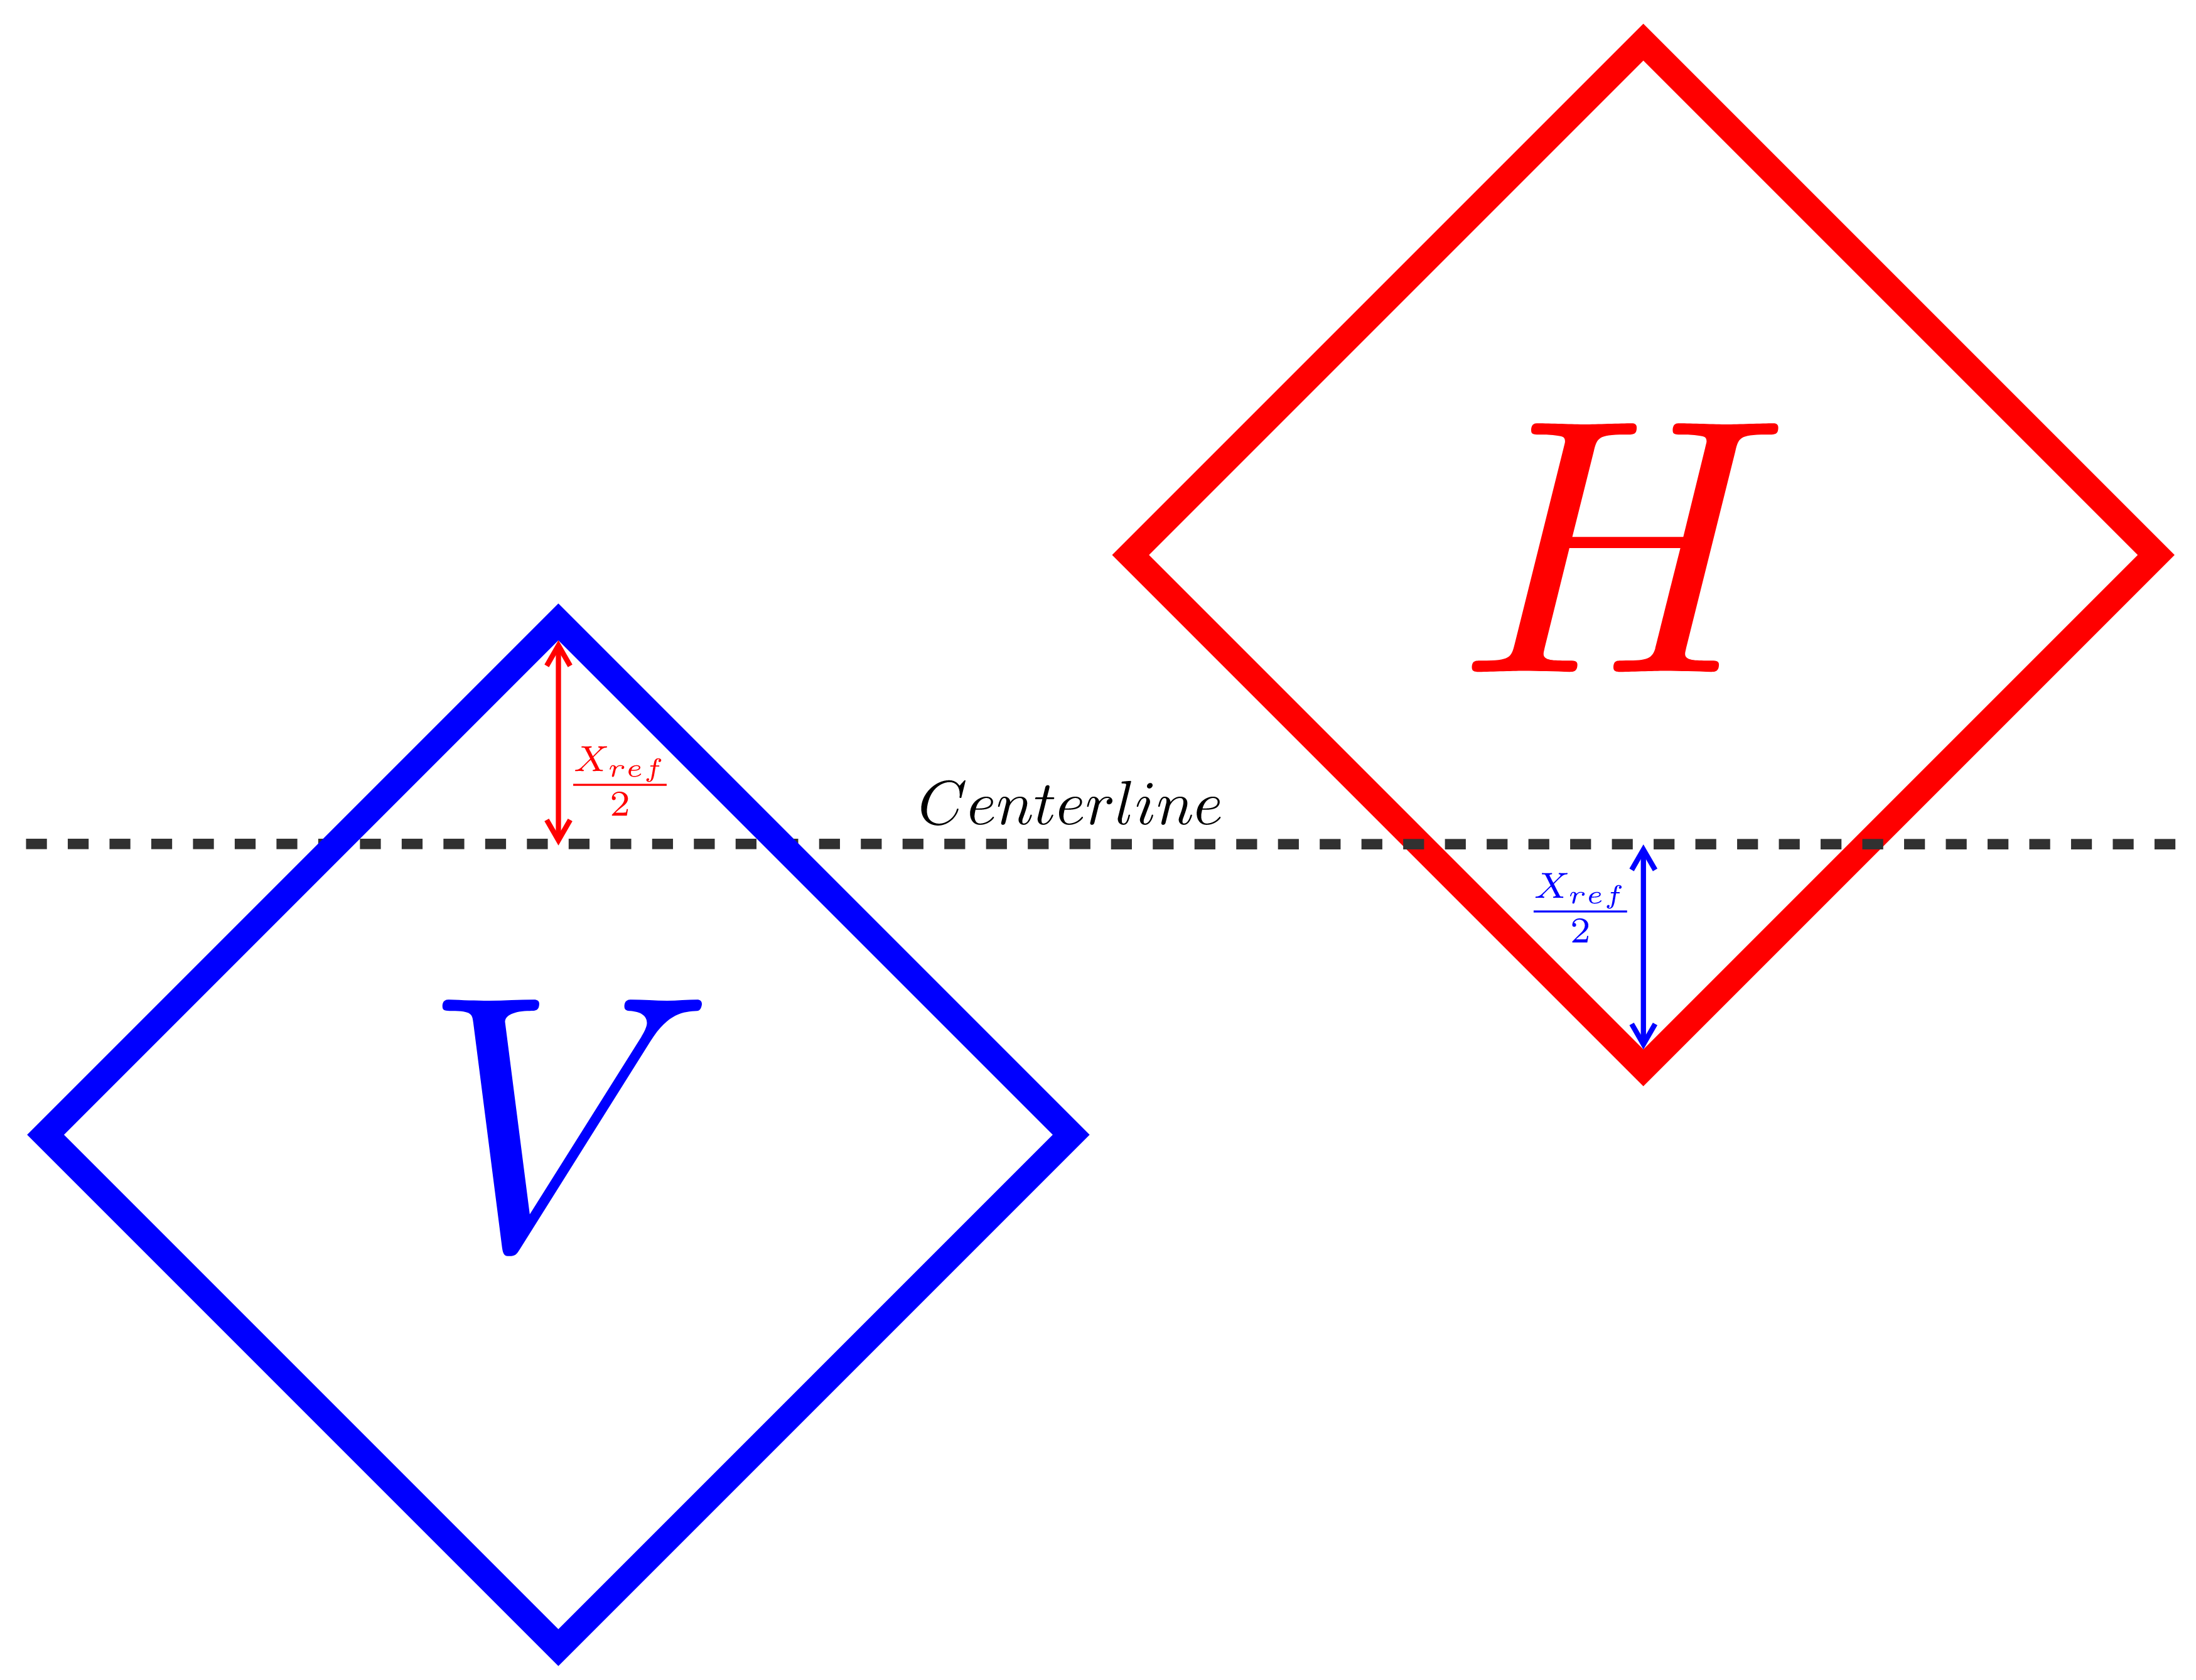
\includegraphics[width=0.48\textwidth]{K_pos.png}
				\caption{Orifice geometry}
				\label{fig:K_pos}
			\end{wrapfigure}

			\newpage
			As manufactured, $K_V \ell_{V_0}$ is defined as the distance from the top surface of the Valve Orifice $(y_T)$, whose machined height equals $\ell_{V_0}$, such that

			\begin{equation}
				K_V \ell_{v_0} = \frac{l_{v_0}}{2} - \left[ \frac{X_{ref}}{2} + d_{V_v} \right]
			\end{equation}

			where $d_{V_v}$ is the vertical position error of the EDM operation (defined as positive in the upwards direction), identical to the horizontal position error.

			Likewise, $K_H (2 \ell_{W_0} + \ell_{H_0})$ is defined as the distance from the top surface of the Housing Outlet $(y_0)$, whose machined height equals $(2 \ell_{W_0} + \ell_{H_0})$, such that

			\begin{equation}
				K_H (2 \ell_{W_0} + \ell_{H_0}) = \frac{(2 \ell_{W_0} + \ell_{H_0})}{2} + \left[ \frac{X_{ref}}{2} - d_{V_v} \right]
			\end{equation}

			therefore

			\begin{align}
				K_V &= \frac{1}{2} - \frac{\frac{X_{ref}}{2} + d \ell_{V_v}}{\ell_{V_0}} \\[6pt]
				K_H &= \frac{1}{2} + \frac{\frac{X_{ref}}{2} - d \ell_{H_v}}{2 \ell_{W_0} + \ell_{H_0}}
			\end{align}

			Note that the machined-length values are exact values as the position of the EDM cut is independent of any dimensional error in the valve orifice or housing outlet.

			Using these constants in equations \eqref{eq:yF} and \eqref{eq:yR}, we find the height of the orifice $X$ by taking the difference between the position of the upper and lower corners of the orifice:

				\begin{equation}
					X = y_F - y_R
				\end{equation}

		\newpage

    \subsection{Orifice Geometry}
    \label{app:sat:TF:orif}

			\begin{wrapfigure}{l}{0.35\textwidth}
					\centering
					\includegraphics[width=0.15\textwidth]{G_O.png}
					\caption{Orifice transfer function}
					\label{fig:G_O}
			\end{wrapfigure}

			Finally, with the height of the orifice, we can calculate its effective diameter.
			This is the most critical part of the System Transfer Function because the square orifice bears the most potential for machining errors.
			Such errors will be kept symbolic for now.

			The orifice transfer function $\hat{G}_O$ is best divided into two sub-transfer functions, as in Figure~\ref{fig:G_O}:
			one to convert the orifice into the orifice area $A$, and one to convert area into effective diameter $D_{eff}$.

			\subsubsection{$\hat{G}_A$: Height to Area}
			\label{app:sat:TF:orif:G_A}

				Under ideal machining conditions, the orifice area is calculated as follows:

				\begin{equation}
					A = s^2 = \left( \frac{X}{\sqrt{2}} \right)^2 = \frac{X^2}{2}
				\end{equation}

				Each fillet radius $R_f$ subtracts the following area from the orifice, depicted in Figure~\ref{fig:Rf}:

				\begin{equation}
					dA = (\textit{Orange area}) = (\textit{Square area}) - (\textit{Gray quarter circle}) = R_f^2 - \frac{1}{4} \pi R_f^2 = \frac{1}{4} (4 - \pi) R_f^2
				\end{equation}

				\begin{figure}[H]
					\centering
					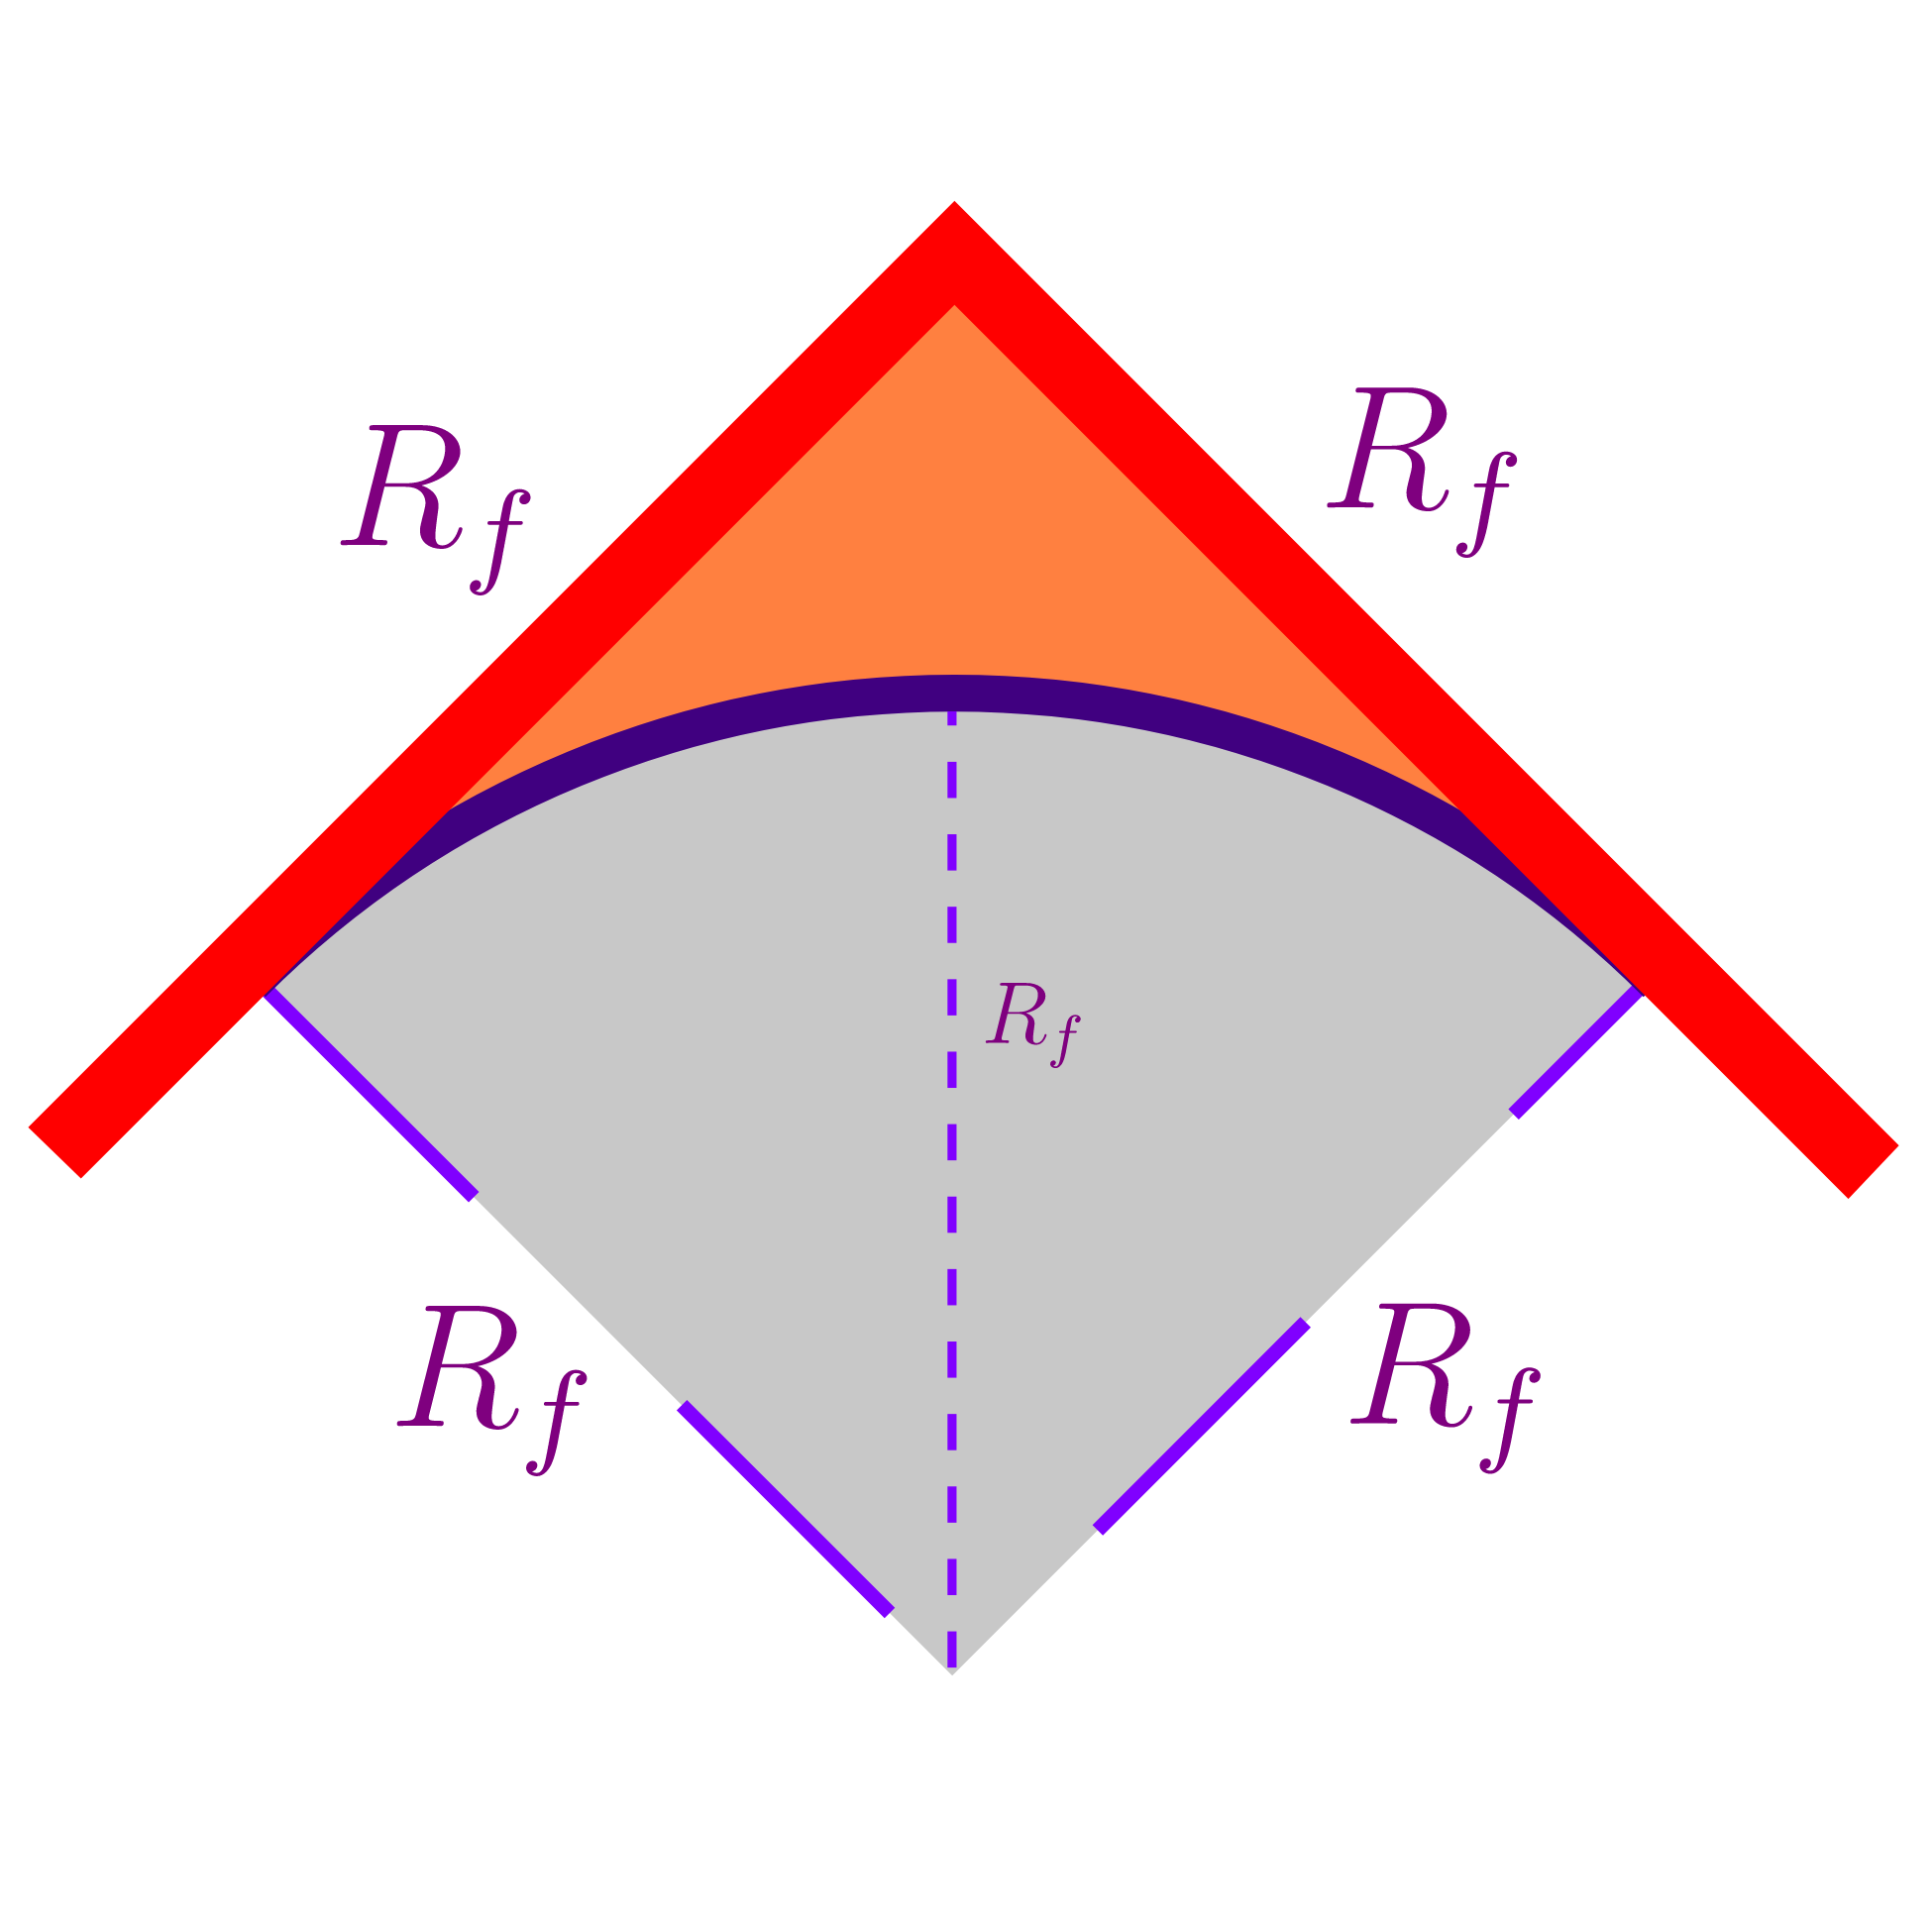
\includegraphics[width=.3\textwidth]{Rf.png}
					\caption{Fillet Radius Dimensions}
					\label{fig:Rf}
				\end{figure}

				Horizontal shift $d \ell_h$ changes the area as shown in Figure~\ref{fig:dl_h}, adding the green area and subtracting the orange.
				Ignoring the fillet radii, this results in the new area

				\begin{equation}
					A = (s + \frac{d \ell}{2}) (s - \frac{d \ell}{2}) = s^2 - \frac{d \ell^2}{2}
				\end{equation}

				\begin{figure}[H]
					\centering
					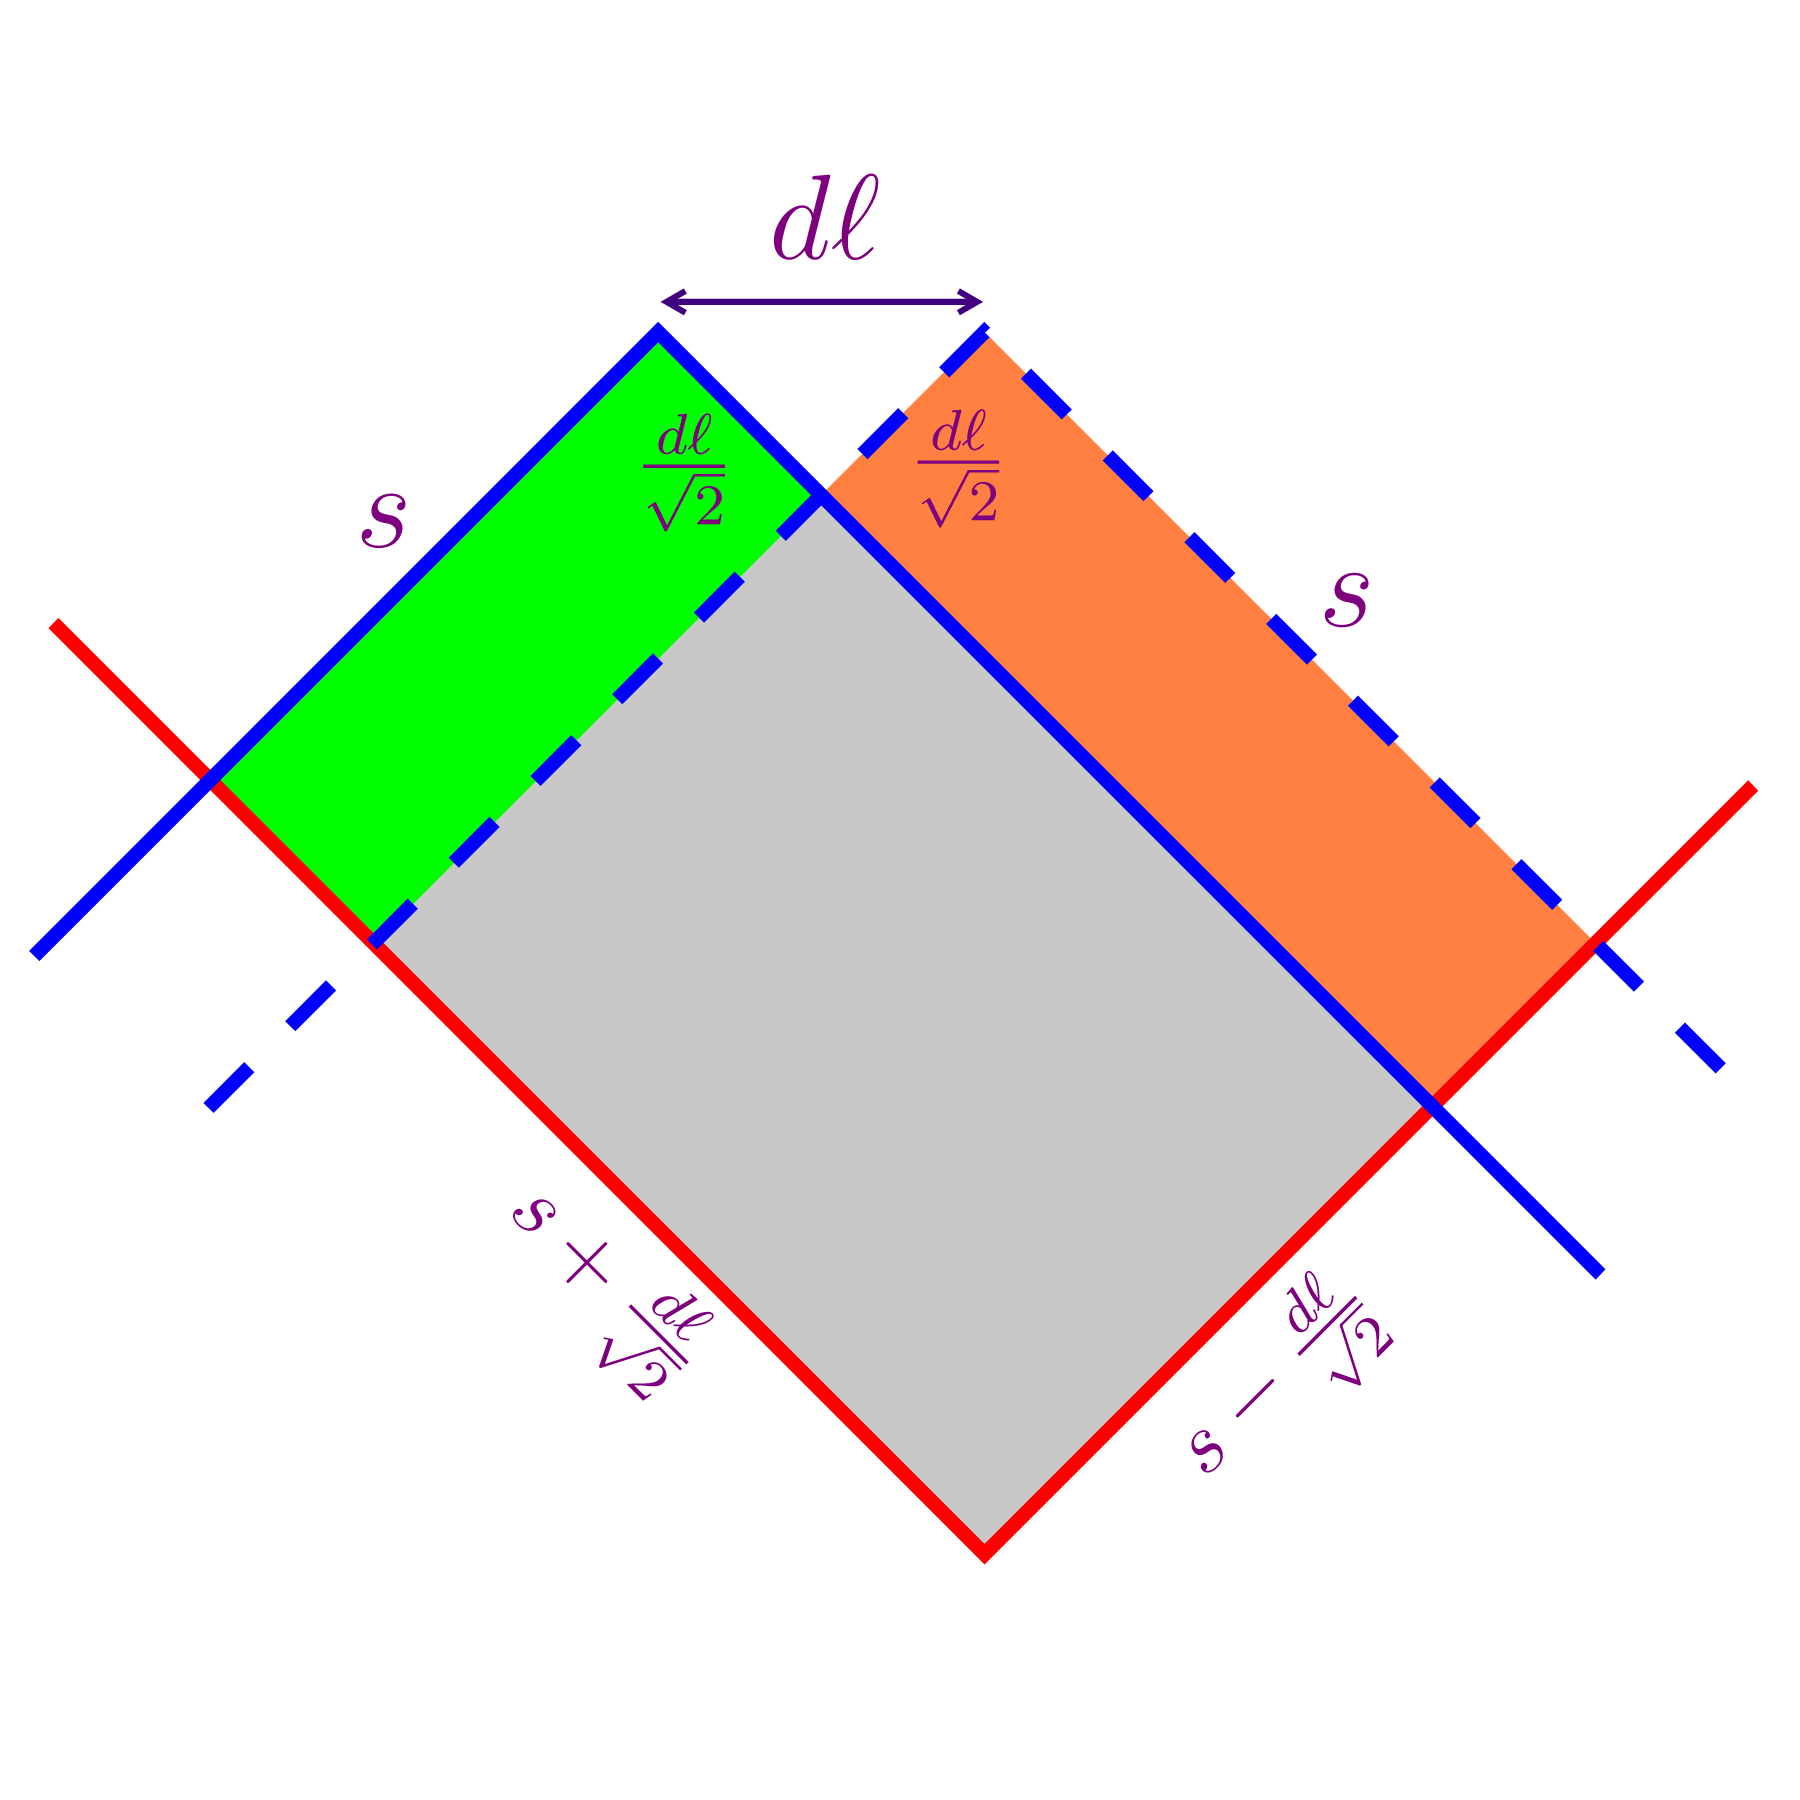
\includegraphics[width=.3\textwidth]{dl_h.png}
					\caption{Horizontal Offset Dimensions}
					\label{fig:dl_h}
				\end{figure}

				yielding the final orifice area:

				\begin{equation}
					A = s^2 - \frac{1}{2} \left[ (4 - \pi) R_f^2 - d \ell^2 \right]
					\label{eq:GA}
				\end{equation}

				The minimum achievable fillet radius and positional tolerance are \SI{76.2}{\micro\meter} and \SI{12.7}{\micro\meter},
				as quoted by Milco Wire EDM, Inc (Appendix~\ref{app:BOM}). These are input into the Transfer Function when numerically evaluated.

			\subsubsection{$\hat{G}_D$: Area to Effective Diameter}
			\label{app:sat:TF:orif:G_D}
				
				The area-diameter conversion is a simple geometric calculation, where $D_{eff}$ is the diameter of a circle with equivalent area. Thus,

				\begin{equation}
					D_{eff} = \sqrt{\frac{4}{\pi} A}
				\end{equation}

			therefore

				\begin{equation}
					\hat{G}_O = \sqrt{\frac{4}{\pi} \left( s^2 - \frac{1}{2} \left[ (4 - \pi) R_f^2 - d \ell^2 \right] \right)}
				\end{equation}

		\subsection{Transfer Function Results}
		\label{app:sat:TF:results}

			The System Transfer Function can be computed using a simple script, which calculates each sub-transfer function as derived above and the force balance using a matrix solver.
			The script was tested with ideal conditions; its output matched the Required Relationship exactly at every temperature.
			Error was then input into the function. Some errors are deterministic or demonstrate an objective worst-case values: variations in aluminum's CTE, spring force deflections, the fillet radius, and effective temperatures.
			The rest --- namely, all vertical dimensional errors ($d \ell_M$, $d \ell_A$, $d \ell_S$, $d \ell_V$, $d \ell_H$, and $d \ell_W$)
			and the vertical and horizontal positions of each orifice ($d \ell_{V_v}$, $d \ell_{H_v}$, $d \ell_{V_h}$, and $d \ell_{H_h}$) ---
			are stochastic. In other words, the value of each will vary each time the part is produced due to slight imprecisions in the machining process
			and cannot be exactly predicted.

			Figure~\ref{fig:TF_res} demonstrates the output of the System Transfer Function given two worst-case combinations of the stochastic error values:
			$d \ell_M$, $d \ell_A$, $d \ell_S$, $d \ell_V$, $d \ell_H$, $d \ell_W$, $d \ell_{V_v}$, $d \ell_{H_v}$, $d \ell_{V_h}$, and $d \ell_{H_h}$.
			These serve as the expected boundaries for any system output across prototypes.
			If many identical devices are manufactured, most will achieve their required tolerance without calibration, but some will reach these boundaries and fall outside of tolerance.
			The lower boundary represents the combination of errors where the effective diameter is the smallest --- the valve stem is positioned lower than it should be.
			The upper boundary represents the opposite.

			Each stochastic machining error follows a normal distribution, where its tolerable range holds approximately six standard deviations $(6 \sigma)$ for a typical Computer-Numeric Control (CNC) machine\cite{ref_AIAG2005}.
			Producing a normalized distribution expectation plot via Monte Carlo analysis\cite{ref_figliola},
			which evaluates $10^6$ samples, each with a different random combination of stochastic inputs and finds the resulting error distribution,
			the function demonstrated that 90.6\% of devices are expected to achieve the Required Relationship without needing calibration.
			It output the normalized distribution in Figure~\ref{fig:error_dist}, with a mean of -45.2\% and a standard deviation of 41.5\%, measured as a percentage of the tolerance window at $T_{ref}$ (where the tolerance is narrowest).
			On average, a freshly-assembled device will produce an orifice that is smaller than nominal by half its tolerance window.
			Those that fall outside of tolerance do not exceed their boundary by more than \SI{44.6}{\micro\meter}.
			These can be remedied using the calibration stack, whose range is sufficient to correct the maximum errors anticipated by the Transfer Function.

			\begin{figure}[h]
				\centering
				\begin{tikzpicture}
				\begin{axis}[
								width       = 14cm,
								height      = 8cm,
								xlabel      = {Ambient Temperature ($^\circ$C)},
								ylabel      = {Actual Effective Diameter ($\upmu$m)},
								xmin = -70, xmax = 90,
								ymin = 80,  ymax = 450,
								grid        = major,
								major grid style = {line width=0.4pt, draw=gray!50},
								minor tick num   = 0,
								tick align  = inside,
								legend pos  = north east,
								legend style     = {font=\small},
								tick label style = {font=\small},
								label style      = {font=\small},
				]

				%% ── Gold TF paths (named, no fill yet) ────────────────────────────────
				\addplot [
								name path   = TF_high,
								color       = ucdgold,
								line width  = 1.6pt,
								dash dot,
								forget plot,
				] table [
								x expr      = \thisrow{T_amb_C},
								y expr      = \thisrow{D_TF_high} * 1e6,
								col sep     = comma,
				] {csv/TF.csv};

				\addplot [
								name path   = TF_low,
								color       = ucdgold,
								line width  = 1.6pt,
								dashed,
								forget plot,
				] table [
								x expr      = \thisrow{T_amb_C},
								y expr      = \thisrow{D_TF_low} * 1e6,
								col sep     = comma,
				] {csv/TF.csv};

				%% ── Gold fill ─────────────────────────────────────────────────────────
				\addplot [
								fill        = ucdgold!20,
								draw        = none,
								forget plot,
				] fill between [of = TF_high and TF_low];

				%% ── Blue tolerance paths (named, no fill yet) ─────────────────────────
				\addplot [
								name path   = lower,
								color       = ucdblue,
								line width  = 0.8pt,
								dotted,
								forget plot,
				] table [
								x expr      = \thisrow{T_amb_C},
								y expr      = \thisrow{D_eff_lower} * 1e6,
								col sep     = comma,
				] {csv/TF.csv};

				\addplot [
								name path   = upper,
								color       = ucdblue,
								line width  = 0.8pt,
								dotted,
								forget plot,
				] table [
								x expr      = \thisrow{T_amb_C},
								y expr      = \thisrow{D_eff_upper} * 1e6,
								col sep     = comma,
				] {csv/TF.csv};

				%% ── Blue fill (on top of gold) ────────────────────────────────────────
				\addplot [
								fill        = sandiablue!20,
								draw        = none,
								forget plot,
				] fill between [of = lower and upper];

				%% ── Nominal required line ─────────────────────────────────────────────
				\addplot [
								color       = ucdblue,
								line width  = 1.6pt,
								forget plot,
				] table [
								x expr      = \thisrow{T_amb_C},
								y expr      = \thisrow{D_eff_nominal} * 1e6,
								col sep     = comma,
				] {csv/TF.csv};

				%% ── Monte Carlo mean output (all stochastic errors = 0, R_f applied) ──
				\addplot [
								color       = ucdgold,
								line width  = 1.6pt,
								solid,
								forget plot,
				] table [
								x expr      = \thisrow{T_amb_C},
								y expr      = \thisrow{D_TF_mean} * 1e6,
								col sep     = comma,
				] {csv/TF.csv};

				%% ── Legend entries ────────────────────────────────────────────────────
				\addplot [color=ucdblue, line width=1.6pt]
								coordinates {(-200,0)};
				\addlegendentry{Nominal output}

				\addplot [color=ucdblue, line width=0.8pt, dotted]
								coordinates {(-200,0)};
				\addlegendentry{Tolerance band}

				\addplot [color=ucdgold, line width=1.6pt, solid]
								coordinates {(-200,0)};
				\addlegendentry{Mean output}

				\addplot [color=ucdgold, line width=1.6pt, dash dot]
								coordinates {(-200,0)};
				\addlegendentry{Stochastic boundaries}

				\end{axis}
				\end{tikzpicture}%
				\caption{Transfer Function Output}
				\label{fig:TF_res}
			\end{figure}

			\vspace{1em}
			\begin{figure}[h]
					\centering
					\begin{tikzpicture}
					\begin{axis}[
							width       = 14cm,
							height      = 8cm,
							xlabel      = {Error (\% tolerance window at $T_{ref}$)},
							ylabel      = {Probability Density},
							xmin = -250, xmax = 150,
							ymin = 0,    ymax = 0.011,
							grid        = major,
							major grid style = {line width=0.4pt, draw=gray!50},
							minor tick num   = 0,
							tick align  = inside,
							tick label style = {font=\small},
							label style      = {font=\small},
							yticklabel style = {
									/pgf/number format/precision=4,
							},
					]

					%% ── ±100% tolerance window background ───────────────────────────────────
					\addplot [
							name path = tol_lo,
							draw      = none,
							domain    = -100:100,
							samples   = 2,
							forget plot,
					] {0};
					\addplot [
							name path = tol_hi,
							draw      = none,
							domain    = -100:100,
							samples   = 2,
							forget plot,
					] {0.011};
					\addplot [
							fill       = ucdgold!18,
							draw       = none,
							forget plot,
					] fill between [of = tol_lo and tol_hi];

					%% ── ±2σ shaded band ──────────────────────────────────────────────────────
					% ±2σ bounds: μ ± 2σ = -45.1746 ± 83.0826 → [-128.257, 37.908]
					\addplot [
							name path = twosig_lo,
							draw      = none,
							domain    = -128.257:37.908,
							samples   = 2,
							forget plot,
					] {0};
					\addplot [
							name path = twosig_hi,
							draw      = none,
							domain    = -128.257:37.908,
							samples   = 200,
							forget plot,
					] {normalpdf(x, -45.1746, 41.5413)};
					\addplot [
							fill       = sandiablue!15,
							draw       = none,
							forget plot,
					] fill between [of = twosig_lo and twosig_hi];

					%% ── ±1σ shaded band ──────────────────────────────────────────────────────
					% ±1σ bounds: μ ± σ = -45.1746 ± 41.5413 → [-86.716, -3.633]
					\addplot [
							name path = onesig_lo,
							draw      = none,
							domain    = -86.716:-3.633,
							samples   = 2,
							forget plot,
					] {0};
					\addplot [
							name path = onesig_hi,
							draw      = none,
							domain    = -86.716:-3.633,
							samples   = 200,
							forget plot,
					] {normalpdf(x, -45.1746, 41.5413)};
					\addplot [
							fill       = sandiablue!30,
							draw       = none,
							forget plot,
					] fill between [of = onesig_lo and onesig_hi];

					%% ── Normal PDF ───────────────────────────────────────────────────────────
					\addplot [
							color      = ucdgold,
							line width = 1.6pt,
							solid,
							domain     = -250:150,
							samples    = 300,
							forget plot,
					] {normalpdf(x, -45.1746, 41.5413)};

					%% ── σ callout labels ─────────────────────────────────────────────────────
					\node[font=\small, align=center]
							at (axis cs: -45.1746, 0.005)
							{$\pm1\sigma$};

					\node[font=\small, align=center]
							at (axis cs: -105, 0.001)
							{$\pm2\sigma$};
					\node[font=\small, align=center]
							at (axis cs: 15, 0.001)
							{$\pm2\sigma$};

					%% --- Tolerance band --------------------------------
					\node[font=\small, align=center]
							at (axis cs: 0, 0.0102)
							{\textit{Tolerance window}};

					%% --- Percentage compliance ----------------------------
					\node[font=\small, align=center]
							at (axis cs: -45.1746, 0.003)
							{\textit{90.6\%}};
					\node[font=\small, align=center]
							at (axis cs: -45.1746, 0.0023)
							{\textit{compliance}};

					\end{axis}
					\end{tikzpicture}
					\caption{Stochastic Error Distribution}
					\label{fig:error_dist}
			\end{figure}

			As detailed in Appendix~\ref{app:mfg}, calibration will be performed at approximately $T_{ref}$.
			The maximum expected error at this temperature, as calculated by the Transfer Function, is \SI{30.7}{\micro\meter} and \SI{44.6}{\micro\meter} above and below the nominal reference diameter of

			\begin{equation}
				\Dref
			\end{equation}

			At a minimum, the calibration assembly must be able to correct the error at the extrema by the largest deviation value to the specified tolerance. Thus,

			\begin{equation}
				\Delta D_{cal} \geq 45 \pm 12.7\si{\micro\meter}
			\end{equation}

			Assuming exactly these calibration capabilities, the Transfer Function evaluated the new system output boundaries.
			As shown in Figure~\ref{fig:TF_cal}, these now fall just within the required tolerance window despite several persistent sources of error.
			As discussed in Section~\ref{app:calcs:cal:sat}, the user will likely be able to exceed this tolerance, resulting in a system output well within the required tolerance across the whole temperature range.

			Although calibration corrects the static offset introduced by the vertical dimension errors that affect the orifice height, several errors persist after calibration that change the temperature-diameter slope or introduce nonlinearity.

			\begin{enumerate}
				\item Deviation from the assumed \SI{50}{\micro\meter} compression of the belleville washer will effectively change the mount's machined length, allowing the mount to expand or contract slightly more or less than designed.
					This cannot be avoided. The function accounted for this change when producing Figure~\ref{fig:TF_cal}; it accounts for the erroneous initial slopes.
					At colder temperatures, where the diameter is larger and nonlinear errors (discussed below) take less effect, one can see that the upper bound slopes away from the nominal output.
					This represents devices whose diameter has been reduced by calibration, decompressing the belleville washer and shrinking the mount's expandible length.
					The effective diameter decreases slightly less than required because the mount provides slightly less actuation.
					One would expect the lower bound to exhibit the opposite effect, its mount having been increased by washer compression.
					However, it follows a similar, though subtler, shallow initial slope before being pull downwards by the orifice machining errors.
					The source of this discrepancy is not certain.
				\item The fillet radius and horizontal position error cannot be corrected. These subtract a constant area, disproportionately reducing the effective diameter towards the hotter temperatures, where the diameter is smallest.
					One can see its effect on the right side of Figure~\ref{fig:TF_cal}, where the expected output diameter drops off at an increasing rate.
					Those devices that produce too large a diameter will conveniently approach the setpoint.
					Those that produce too small a diameter will show greater error on that end, but are expected to remain within tolerance as the window widens toward the extrema.
					The effect is negligible, but if future iterations require compensation for higher temperatures with a smaller diameter, better methods will need to be developed to correct or reduce this error mode.
			\end{enumerate}

			\begin{figure}[H]
					\centering
					\begin{tikzpicture}
					\begin{axis}[
							width       = 14cm,
							height      = 8cm,
							xlabel      = {Ambient Temperature ($^\circ$C)},
							ylabel      = {Actual Effective Diameter ($\upmu$m)},
							xmin = -70, xmax = 90,
							ymin = 80,  ymax = 450,
							grid        = major,
							major grid style = {line width=0.4pt, draw=gray!50},
							minor tick num   = 0,
							tick align  = inside,
							legend pos  = north east,
							legend style     = {font=\small},
							tick label style = {font=\small},
							label style      = {font=\small},
					]

					%% ── Gold TF calibrated paths (named, no fill yet) ─────────────────────
					\addplot [
							name path   = TF_high_cal,
							color       = ucdgold,
							line width  = 1.6pt,
							dash dot,
							forget plot,
					] table [
							x expr      = \thisrow{T_amb_C},
							y expr      = \thisrow{D_TF_high_cal} * 1e6,
							col sep     = comma,
					] {csv/TF_cal.csv};

					\addplot [
							name path   = TF_low_cal,
							color       = ucdgold,
							line width  = 1.6pt,
							dashed,
							forget plot,
					] table [
							x expr      = \thisrow{T_amb_C},
							y expr      = \thisrow{D_TF_low_cal} * 1e6,
							col sep     = comma,
					] {csv/TF_cal.csv};

					%% ── Gold fill ─────────────────────────────────────────────────────────
					\addplot [
							fill        = ucdgold!20,
							draw        = none,
							forget plot,
					] fill between [of = TF_high_cal and TF_low_cal];

					%% ── Blue tolerance paths (named, no fill yet) ─────────────────────────
					\addplot [
							name path   = lower_cal,
							color       = ucdblue,
							line width  = 0pt,
							dotted,
							forget plot,
					] table [
							x expr      = \thisrow{T_amb_C},
							y expr      = \thisrow{D_eff_lower} * 1e6,
							col sep     = comma,
					] {csv/TF_cal.csv};

					\addplot [
							name path   = upper_cal,
							color       = ucdblue,
							line width  = 0pt,
							dotted,
							forget plot,
					] table [
							x expr      = \thisrow{T_amb_C},
							y expr      = \thisrow{D_eff_upper} * 1e6,
							col sep     = comma,
					] {csv/TF_cal.csv};

					%% ── Blue fill ─────────────────────────────────────────────────────────
					\addplot [
							fill        = sandiablue!20,
							draw        = none,
							forget plot,
					] fill between [of = lower_cal and upper_cal];

					%% ── Nominal required line ─────────────────────────────────────────────
					\addplot [
							color       = ucdblue,
							line width  = 1.6pt,
							forget plot,
					] table [
							x expr      = \thisrow{T_amb_C},
							y expr      = \thisrow{D_eff_nominal} * 1e6,
							col sep     = comma,
					] {csv/TF_cal.csv};

					%% ── Legend entries ────────────────────────────────────────────────────
					\addplot [color=ucdblue, line width=1.6pt]
							coordinates {(-200,0)};
					\addlegendentry{Nominal output}

					\addplot [color=ucdblue, line width=0.8pt, dotted]
							coordinates {(-200,0)};
					\addlegendentry{Tolerance band}

					\addplot [color=ucdgold, line width=1.6pt, dash dot]
							coordinates {(-200,0)};
					\addlegendentry{Calibrated boundaries}

					\end{axis}
					\end{tikzpicture}%
					\caption{Transfer Function Output After Calibration}
					\label{fig:TF_cal}
			\end{figure}

			The Tranfer Function accomplishes two objectives. First, it demonstrates the viability of the \device\ despite its strict output requirement. 90\% of manufactured devices are expected to meet their
			tolerance window; those that do not can be readily calibrated. As is addressed in Section~\ref{subsec:DFMEA::tol} and Chapter~\ref{chap:concl}, this computation does not account for all sources of error and therefore presents an optimistic
			expectation value for the system performance. However, it verifies that the major anticipated errors have been mitigated to a tolerable amount by the design strategies illustrated in Section~\ref{sec:design:just}.
			Second, it provides a ready tool for further iteration. Appendix~\ref{app:iter:customize} provides guidance to use this Transfer Function and its associated software to more quickly evaluate the impact of design changes and improvements.

\chapter{Further Failure Analysis and Design Recommendations}

	\section{Design Weaknesses and Recommendations}
	\label{app:iter:weak}

		To aid in further iteration of the \device\ design, below is an exhaustive list of the weaknesses, unaddressed assumptions, and open questions
		identified by the authors and certain corresponding design changes they would implement given more time, excluding those identified in Chapter~\ref{chap:concl}.

		

		\begin{itemize}
			\item The Valve Orifice and Housing Outlet, which each contain one component of the diamond orifice, are pressed flush against one another by a precision fit.
				This flush contact is assumed to only allow flow through the hole cut into the Valve Orifice without allowing leakage around its sides, but this was never verified.
				The tolerance of the fit may need to be adjusted, or addional sealing applied to ensure gas is not allowed to escape into the rectangular cavity of the housing.
			\item The calibration screw may interfere with the expansion of the aluminum actuator due to a difference in expansion rates. This can be solved by shortening the screw, using an aluminum screw, or both.
			\item The strength of the electron-beam welds used for assembly is assumed to be ideal, an assumption defended in Section~\ref{subsec:design:just:weld_analysis}. Though EBW is the most precise weld available, the weld will likely
				be slightly weaker than the original material and may affect thermal expansion and dimensioning around its area, changing the positions and expansion rates of certain parts.
			\item The weldability of dissimilar metals, most especially that of ALLVAR to Invar, should be investigated. The use of fasteners to attach the mount would eliminate the need to weld these metals together
				without sacrificing the precision of their fusion.
			\item As listed in Chapter~\ref{chap:concl}, steps can be taken to improve the thermal isolation and convection of the actuator subsystem. The housing material between the actuator and the internal components
				can be increased, insulating the actuator against conduction. Holes can be cut into the mount to expose the interior, or more complex features cut with wire electric-discharge machining to maximize its convective contact with the ambient air.
			\item Each of the two above items would be better served if the materials of the actuator components were reversed, using an aluminum mount and an ALLVAR core. By positioning the leading orifice above the trailing orifice, the same relationship
				could be achieved with reversed actuation, allowing for a much cheaper actuator and easier machining of the mount to enable the use of fasteners or convection-increasing features.
			\item Choked flow separation at the sharp corners of the orifice may cause undesirable effects. Flow characteristics should be investigated to determine whether the sharp edges should be filleted, which would
				improve flow behavior without degrading the performance of the orifice.
			\item The achievable precision of machined dimensions on Invar should be evaluated to ensure the required tolerances are achievable despite the material's work-hardening property while being machined.
				Extra measures may be required to anneal the part between cuts.
		\end{itemize}

	\section{Iteration Tools}
	\label{app:iter:customize}

		As Sandia implements changes for the second iteration design, the effects of these changes can readily be analyzed using the tools provided in Appendix~\ref{app:sat} and Chapter~\ref{chap:test}.
		Below is a guide for the use of these tools. The computational software will be provided separately to Sandia.
		
		\subsection{COMSOL simulations}
		\label{app:iter:customize:COMSOL}

			The full computational prototype lives in a single file titled "Prototype.mph". Each of the below simulations can be found as denominated within this file.

			\begin{itemize}
				\item \textbf{Pressure Capacity.} To iterate dimensions for optimal internal pressure capacity, use the finite-element stress analysis titled "MBD Study".
				\item \textbf{Flow Characteristics.} To evaluate the effect of the orifice on the gas flow, such as choking, normal shock, and separation, use the fluid-dynamic simulation titled "Flow Study".
				\item \textbf{Heat Transfer.} To analyze the effects of thermal isolation and convection features, use the thermal analysis titled "Heat Transfer Study".
			\end{itemize}

			For each of the above, follow these steps to iterate the design:

			\begin{itemize}
				\item Revise the CAD assembly, provided separately, to reflect the new design dimensions.
				\item Insert into the simulation and set appropriate surface pairs (i.e. identity or contact pairs) to represent physical relations between parts.
				\item Set boundary conditions, such as surface temperatures, pressure parameters, or initial flow conditions. These can be identical to those used for this report or varied as desired.
			\end{itemize}

		\subsection{Transfer Function}
		\label{app:iter:customize:TF}

			The analytical system-performance analysis presented in Appendix~\ref{app:sat:TF} is computed using a single C++ software package titled "TF.cpp". The script is fully documented to provide guidance
			on the use of each part. Follow the derivation given in Appendix~\ref{app:sat:TF} to understand the source of the constants used.
			Directly manipulate variable values to adjust dimensions, errors, and other parameters. The following items can be readily manipulated.
			
			\begin{itemize}
				\item To change the selected bellows as recommended above, manipulate the initial lengths and spring constants given.
				\item To introduce estimated fiction or pressure forces, a constant load can be applied to the force balance in Section~\ref{app:sat:TF:force_balance} with little change to the derivation.
				\item To evaluate the effect of the welds on critical dimensions, the machined lengths can be adjusted to change the thermal-expansion and orifice-position calculations.
					Values can be added in parallel with the machine-tolerance estimations.
			\end{itemize}

		\subsection{Required Relationship Adjustment}
		\label{app:iter:customize:RR}

			Most importantly, the Required Relationship itself can be readily adjusted to adapt the \device\ for particular experiments.
			The architecture is designed to produce a linear relationship between the ambient air temperature and effective orifice diameter,
			depicted visually in Figure~\ref{fig:RR},
			but the slope and intercept of the relation can be adjusted with little effort.

			\subsubsection{Temperature-Diameter Control Derivative}
			\label{app:iter:customize:RR:slope}

				The slope of system ouput, set to the constant $A_1$ in this design, is defined by the critical actuator dimensions as derived in Section~\ref{subsubsec:design:just:TF:act}.
				Assuming a given gap between the base of the actuator and the upper surface of the housing and a given belleville washer compression
				(\SI{5}{\milli\meter} and \SI{50}{\micro\meter} in this design, respectively), the necessary lengths of the Actuator and Mount can be calculated as in equations~\eqref{eq:L_act} and \eqref{eq:L_mount},
				where $\frac{\Delta L}{\Delta T}$ (\SI{1.91}{\micro\meter\per\degreeCelsius} in this report) is set as desired:

				\begin{align*}
					L_{act} &= \frac{\frac{\Delta L}{\Delta T} + (t_{wash} + L_{gap}) \alpha_{mount}}{\alpha_{act} - \alpha_{mount}} \\[12pt]
					&= \frac{\GA + (\SI{5.55}{\milli\meter}) \cdot (\specMountCTE)}{\specActuatorCTE - \specMountCTE} = \specOrigActuatorLength \\[12pt]
					L_{mount} &= L_{act} + t_{wash} + L_{gap} = \SI{38.541}{\milli\meter} 
				\end{align*}

				If a positive slope is desired, such that the orifice grows with a temperature increase, this can be easily achieved by shrinking the valve stem such that the leading orifice rests above the trailing orifice.

			\subsubsection{Reference Diameter}
			\label{app:iter:customize:RR:intercept}

				The intercept of the system output, set to the constant $A_0$ in this design, is defined by the distance between the upper and lower vertices of the orifice as machined (at $T_{ref}$)
				as shown in equation~\eqref{eq:Dref}. The fixed orifice is centered relative to the housing for ease of machining, but the leading orifice can be tuned to obtain a desired reference diameter
				according to the relation

				\begin{equation}
					H_{\ell} = H_t - \sqrt{\frac{\pi}{2}} D_{ref}
				\end{equation}

				where $H_{\ell}$ and $H_t$ are the height of the leading and trailing orifice, respectively, as denoted in the Engineering Drawings in Appendix~\ref{app:drawings}.
\subsection{Comprehensive Failure Analysis}

	Failure modes identified are displayed in the below table, both those defined as critical and other possible modes. 
	Note that of the non-critical modes, some of them require further analysis as development continues.
	Specifically, the modes relating to cyclic thermal and mechanical loading were not analyzed 
	due to time and resource constraints. These modes were not considered priorities for the manufacturing 
	of low-fidelity prototypes. As the device reaches later phases of testing and life cycle analysis must be
	done these fatigue studies will become necessary. Other failure modes such as the housing center wall 
	deformation under pressure load were considered noncritical as other more fragile sections were analyzed
	instead. In the case of the housing center walls, the housing center welds were analyzed, and given the
	stress concentrates on these corners it was deemed more critical to study. This reasoning is true for the
	housing inlet cone, which is not as likely to fail and has less effect on the internal flow than the orifice channel.
	Below is the comprehensive table of design failure modes with priority modes highlighted.

\newpage
	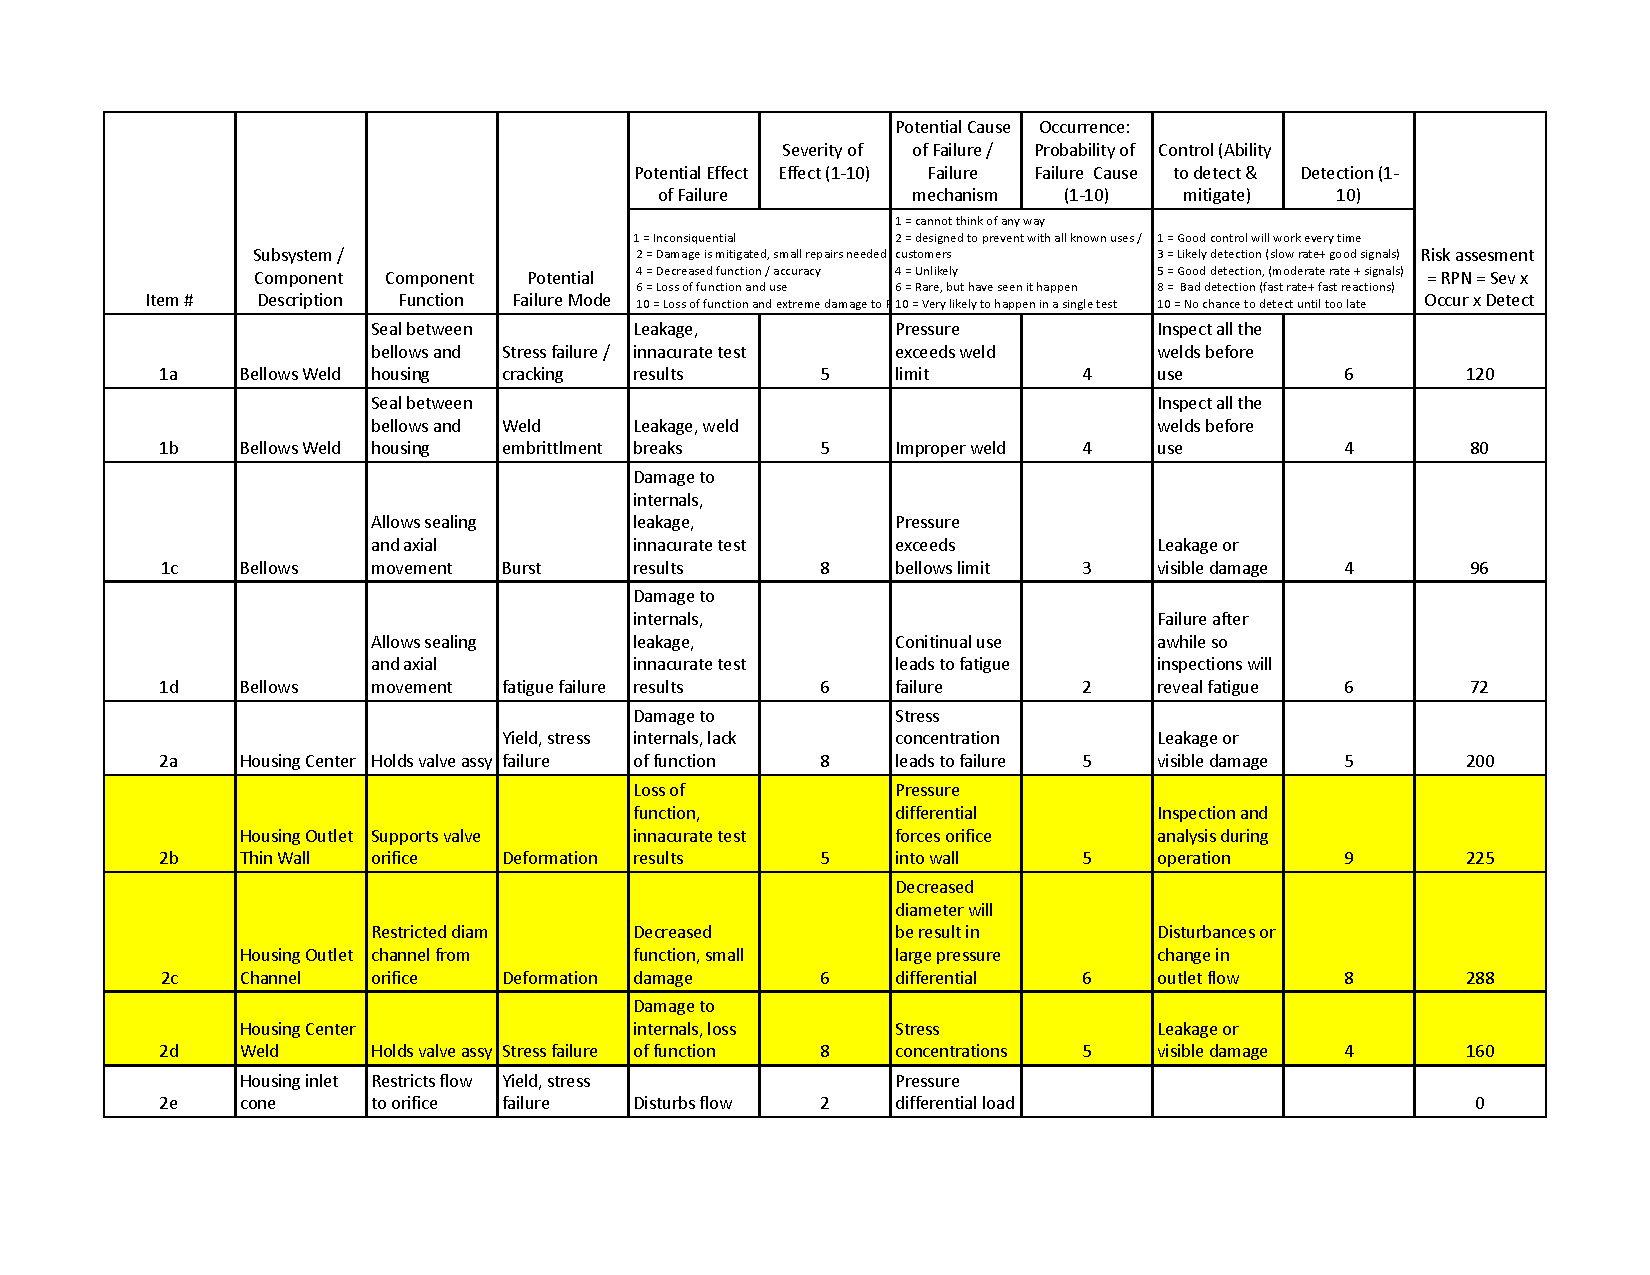
\includepdf[pages=1-2, fitpaper=true, landscape=true]{pdf/DFMEA_table_all.pdf}


\subsection{2 for sam}

\subsection{3 for sam}



\chapter{Complete Bill of Materials}
\label{app:BOM}

	Figures \ref{fig:valve_ID_app} and \ref{fig:act_ID_app} show again the parts needed to manufacture the \device.
	The full Bill of Materials and accompanying vendor quotes are provided on the following pages, with corresponding part numbers, materials, sizes, prices, distributor's links.
	A quote for the Wire Electrical-Discharge Machining (EDM) operation required to cut each square hole is also included from Milco Wire EDM, Inc; achievable tolerance values given in Section~\ref{subsec:DFMEA:error:mach} were taken from this quote.
	A secondary Wire EDM option is provided from Xometry, whose best-achievable fillet radius is \SI{125}{\micro\meter} and whose positional tolerance is as specified in the shop drawings in Appendix~\ref{app:drawings}.

	Data sheets for purchased parts can be found in Appendix~\ref{app:datasheets}.

	\newpage
	\begin{figure}[H]
		\centering
		\includegraphics[height = .4\textheight]{valve_ID.png}
		\caption{Valve Part ID's}
		\label{fig:valve_ID_app}
	\end{figure}
	
	\begin{figure}[H]
		\centering
		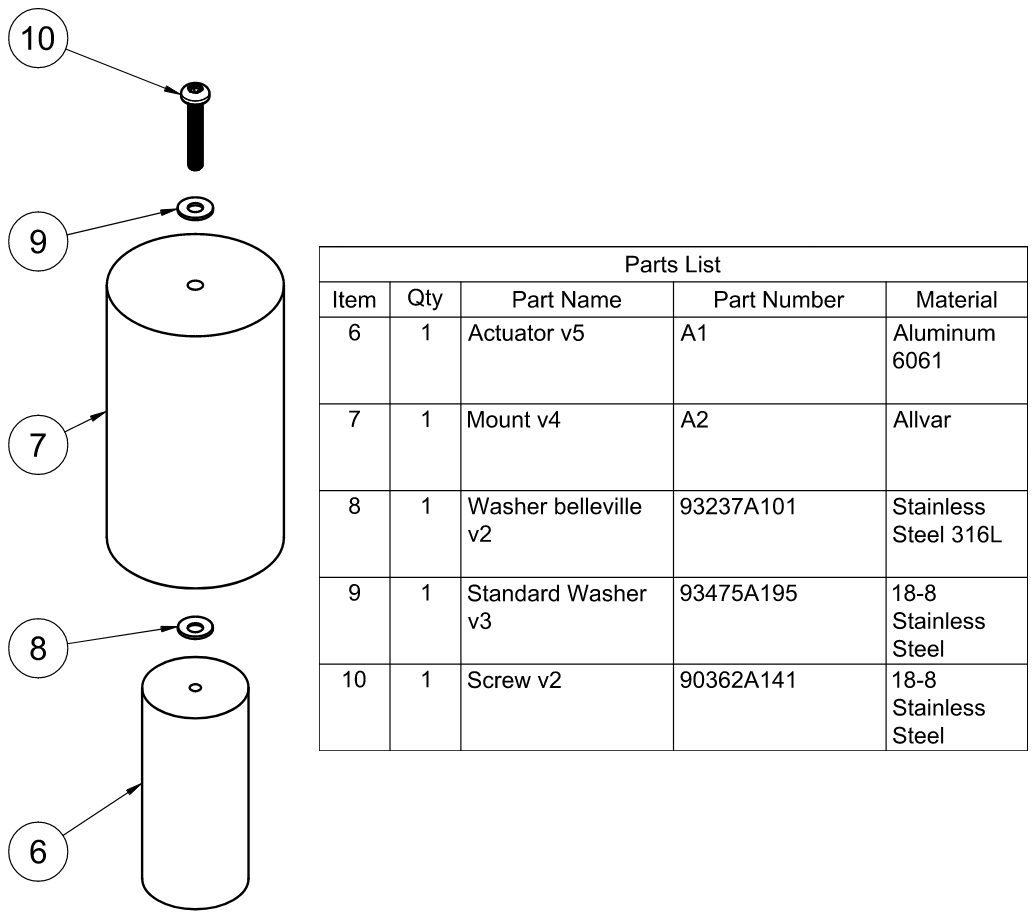
\includegraphics[height = .4\textheight]{Act_ID.png}
		\caption{Actuator Part ID's}
		\label{fig:act_ID_app}
	\end{figure}

	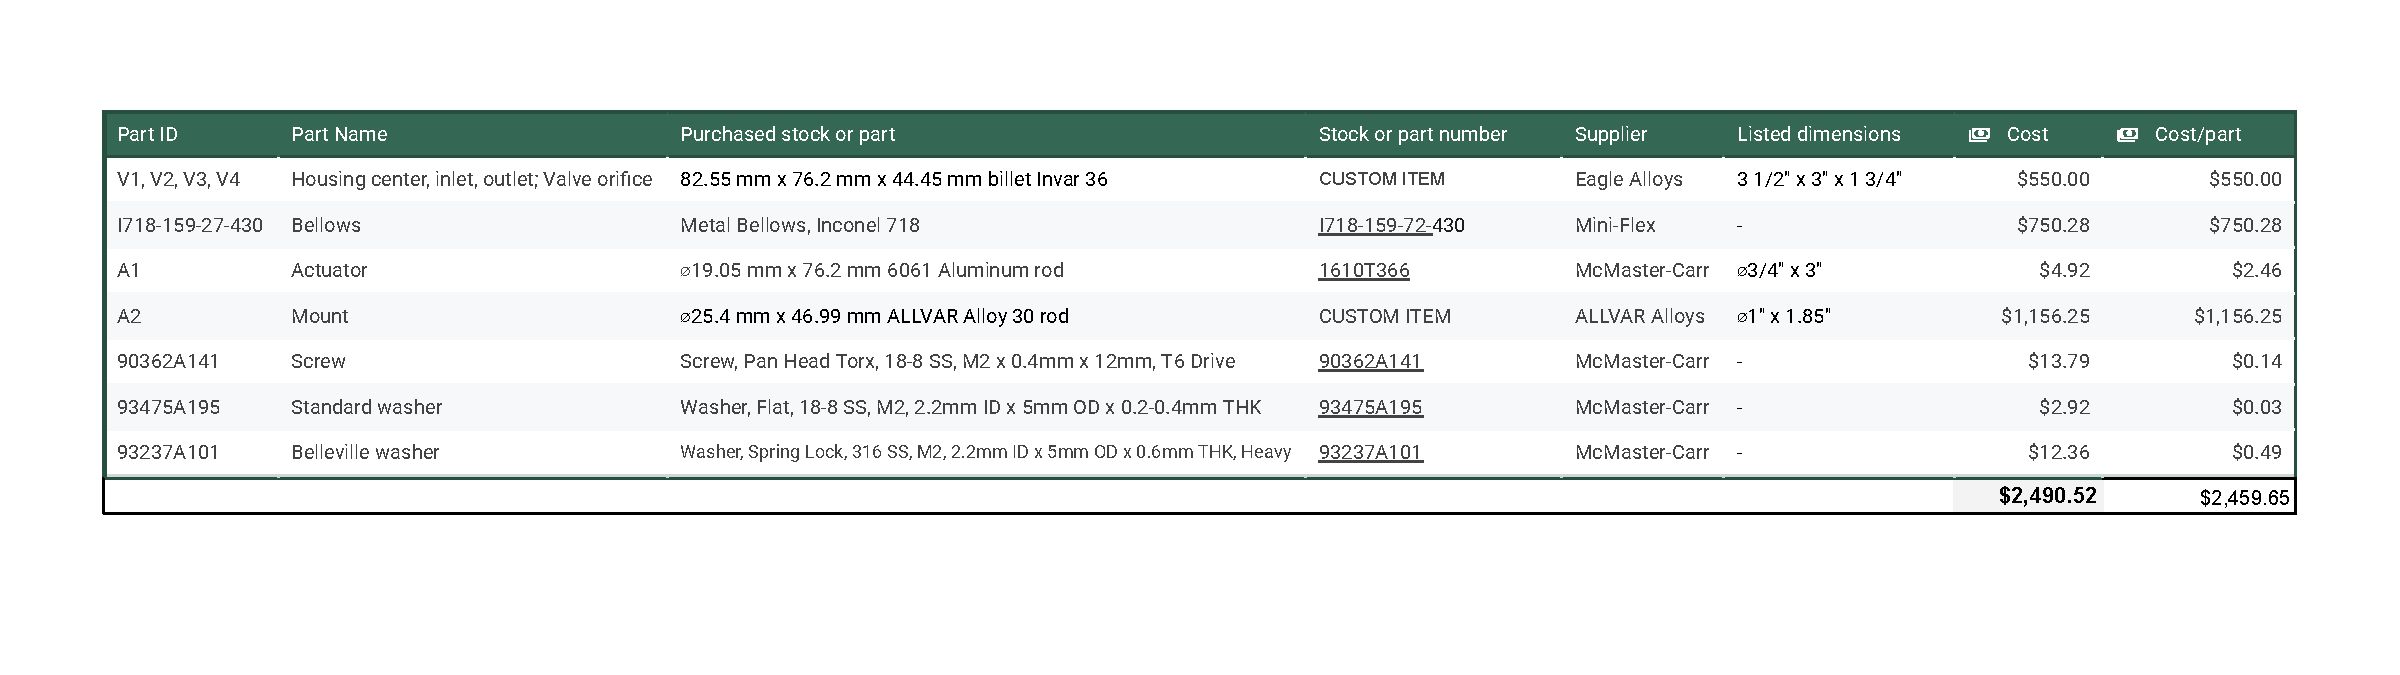
\includepdf[pages=1, fitpaper=true, landscape=true]{pdf/BOM.pdf}

	\newpage
	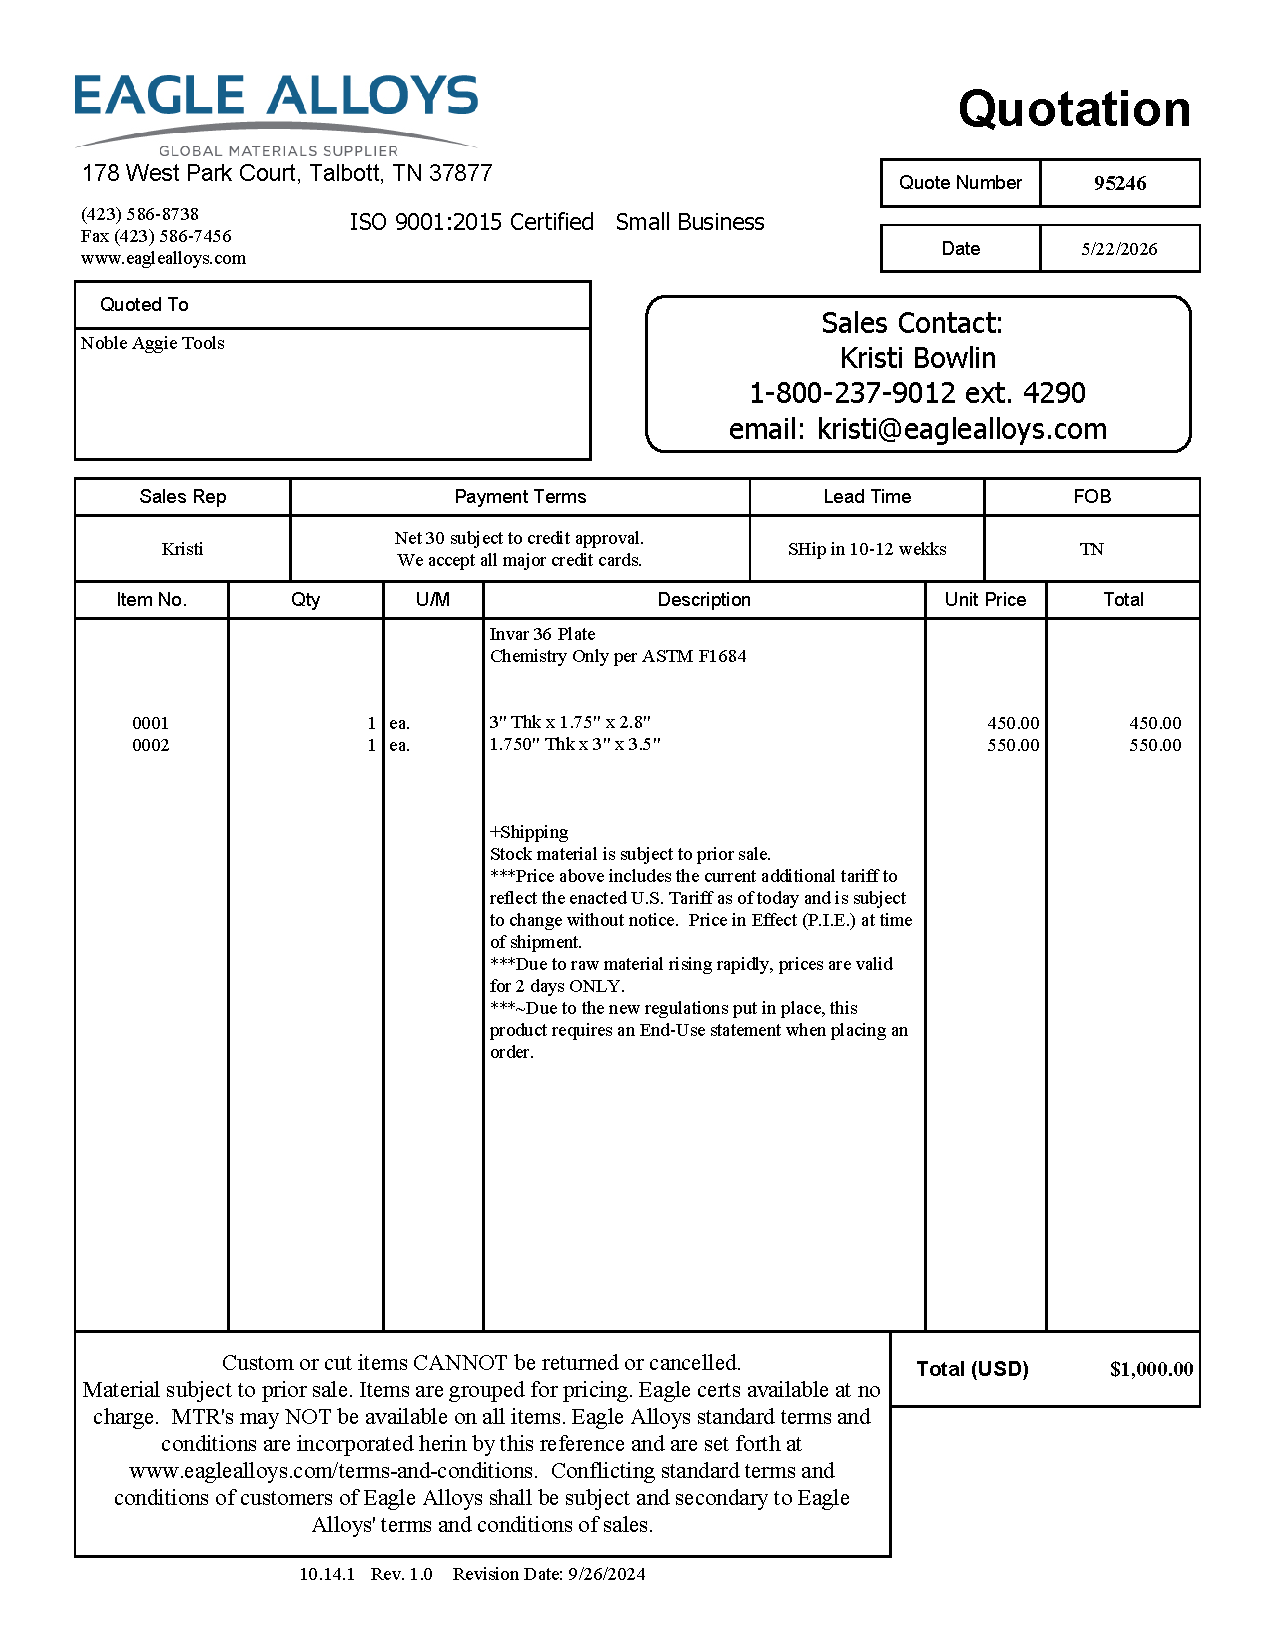
\includepdf[pages=1, fitpaper=true, landscape=true]{pdf/quote_Invar.pdf}
	
	\newpage
	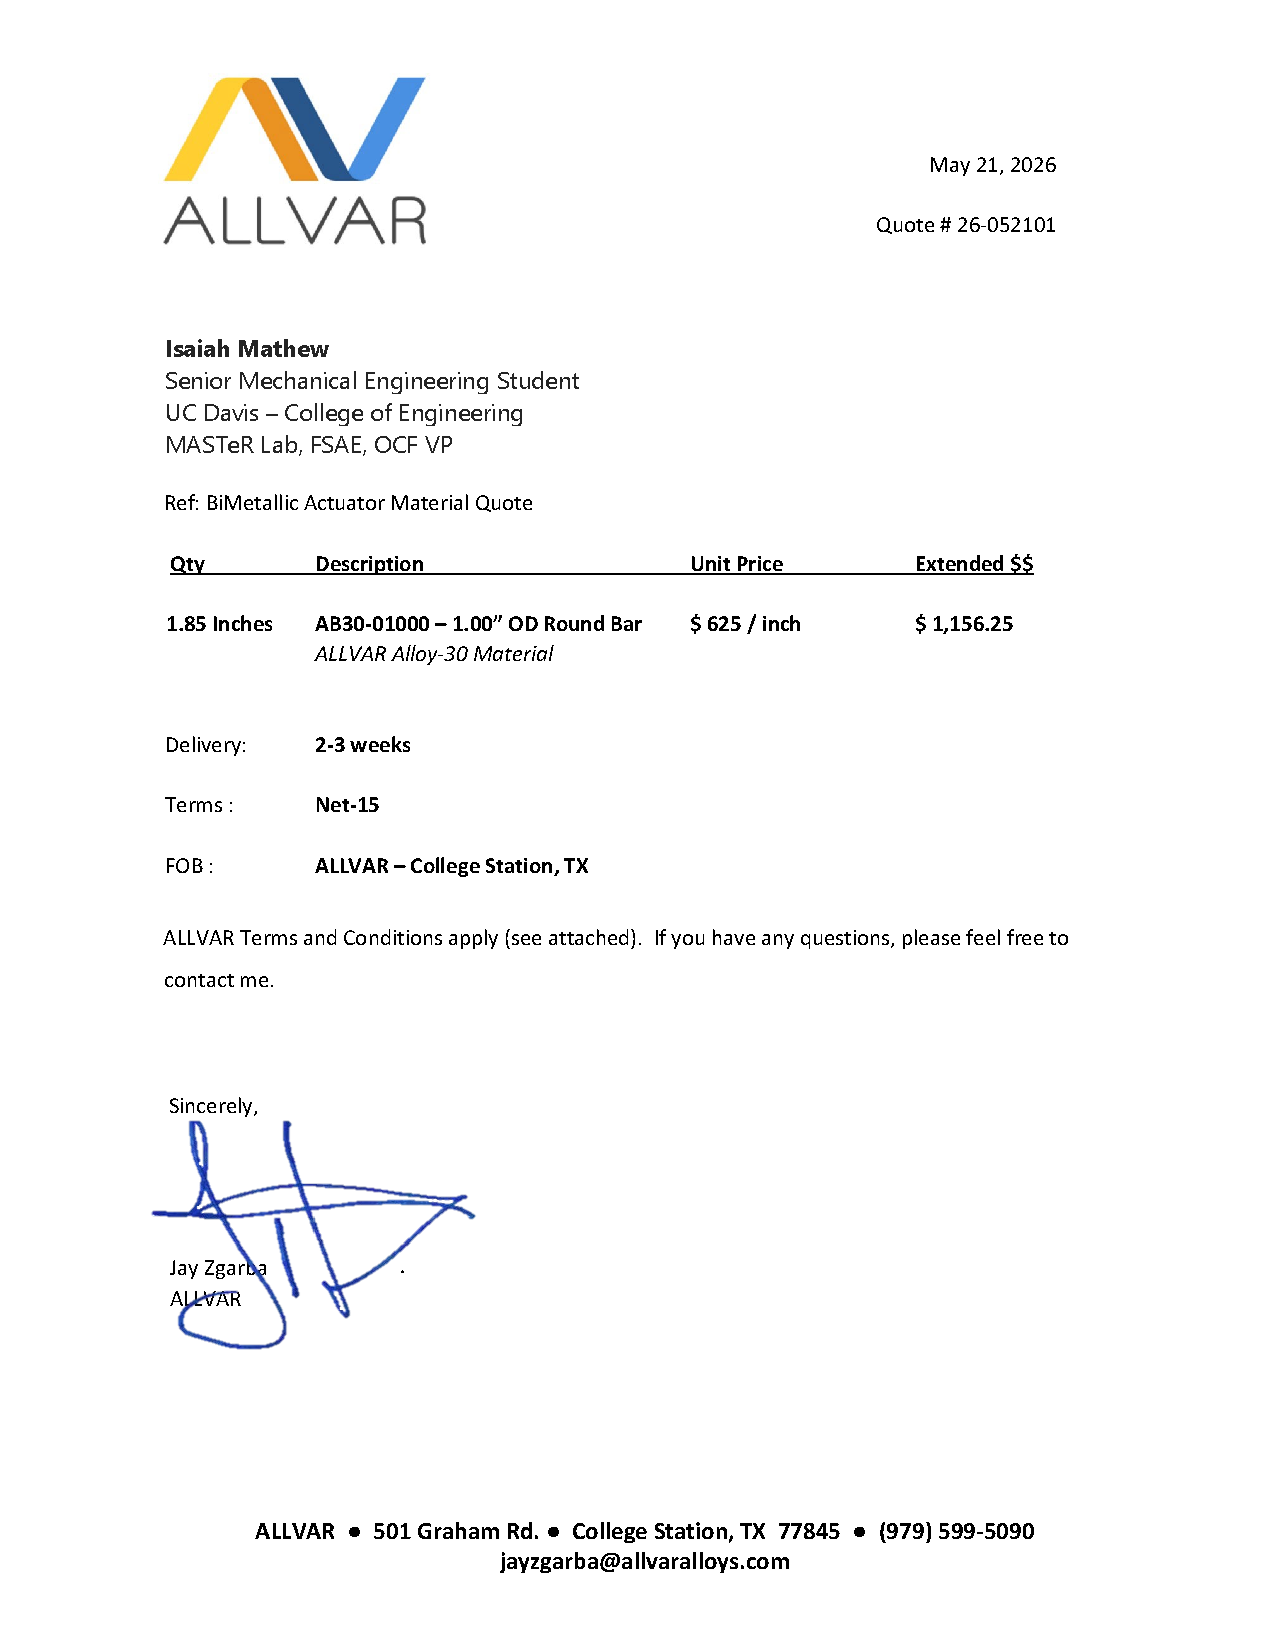
\includepdf[pages=1, fitpaper=true, landscape=true]{pdf/quote_ALLVAR.pdf}
	
	\newpage
	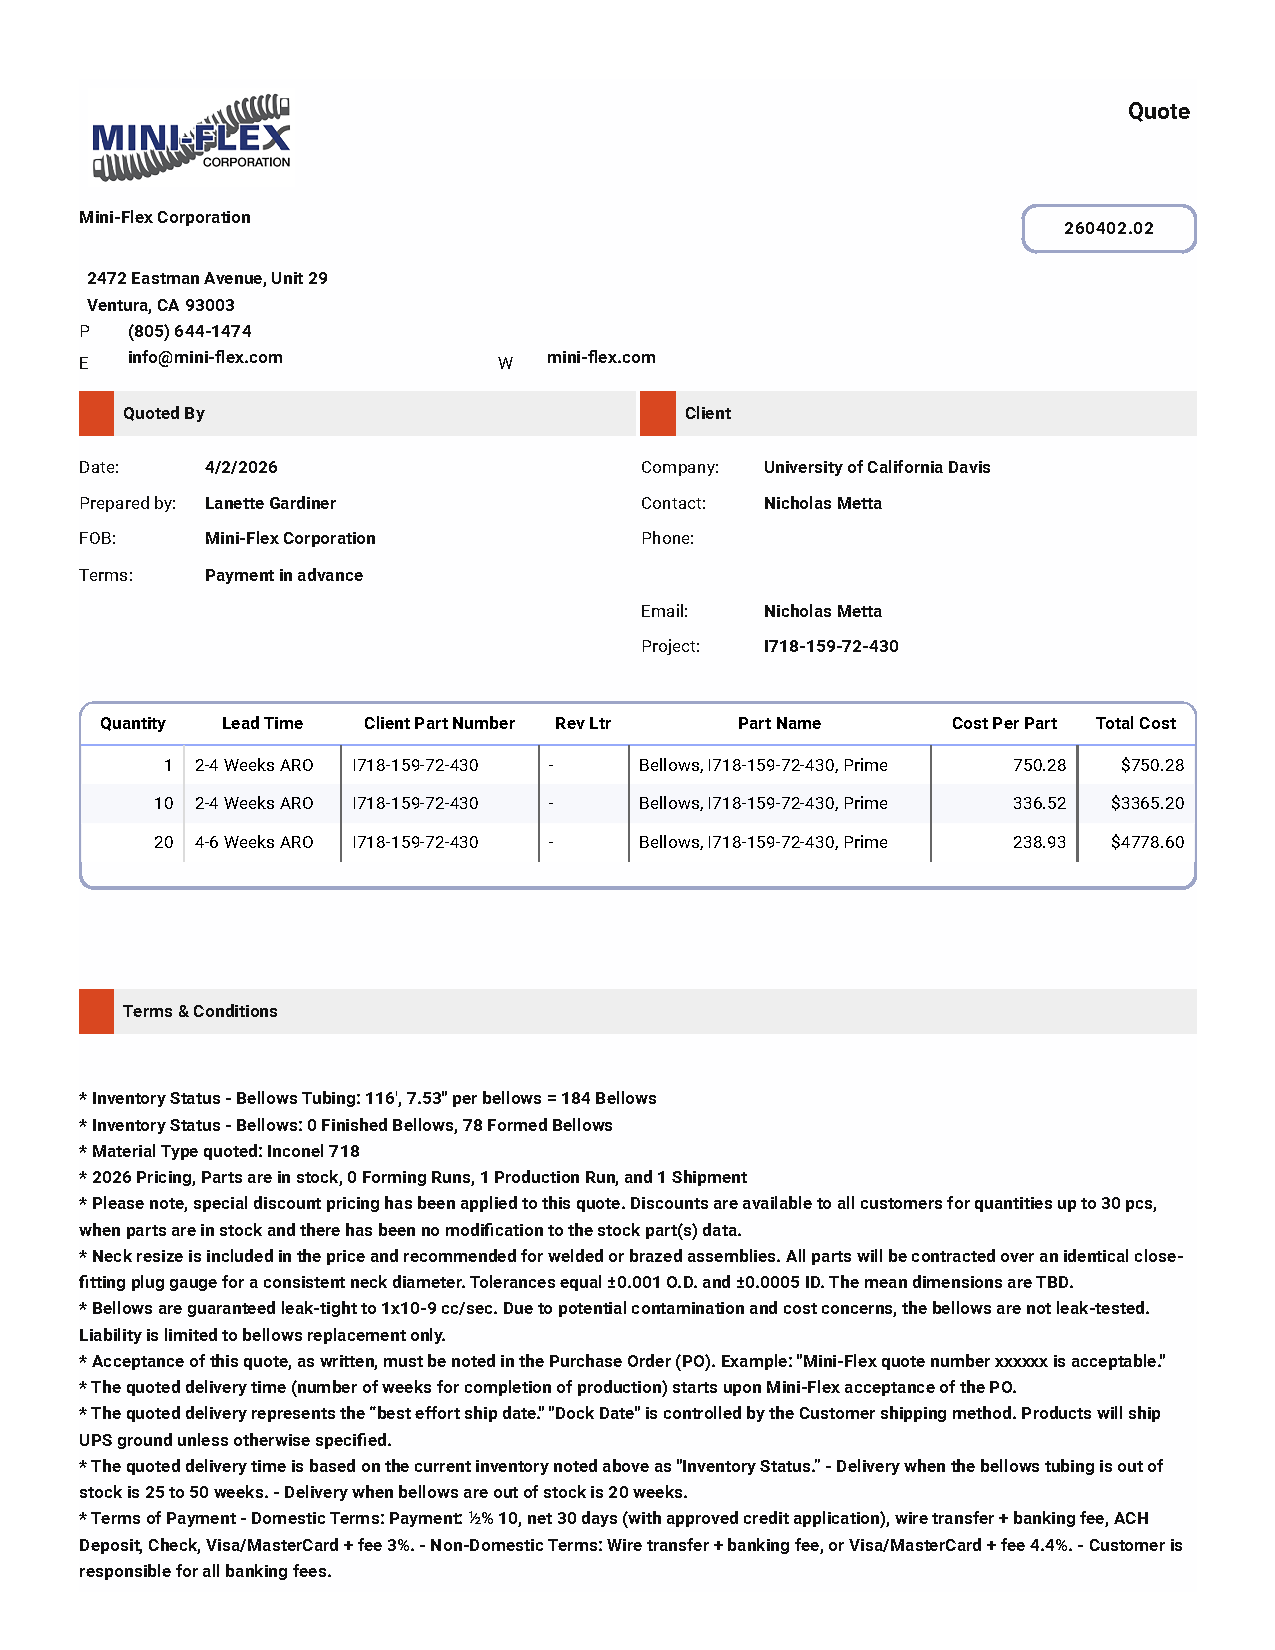
\includepdf[pages=1-2, fitpaper=true, landscape=true]{pdf/quote_bellows.pdf}
	
	\newpage
	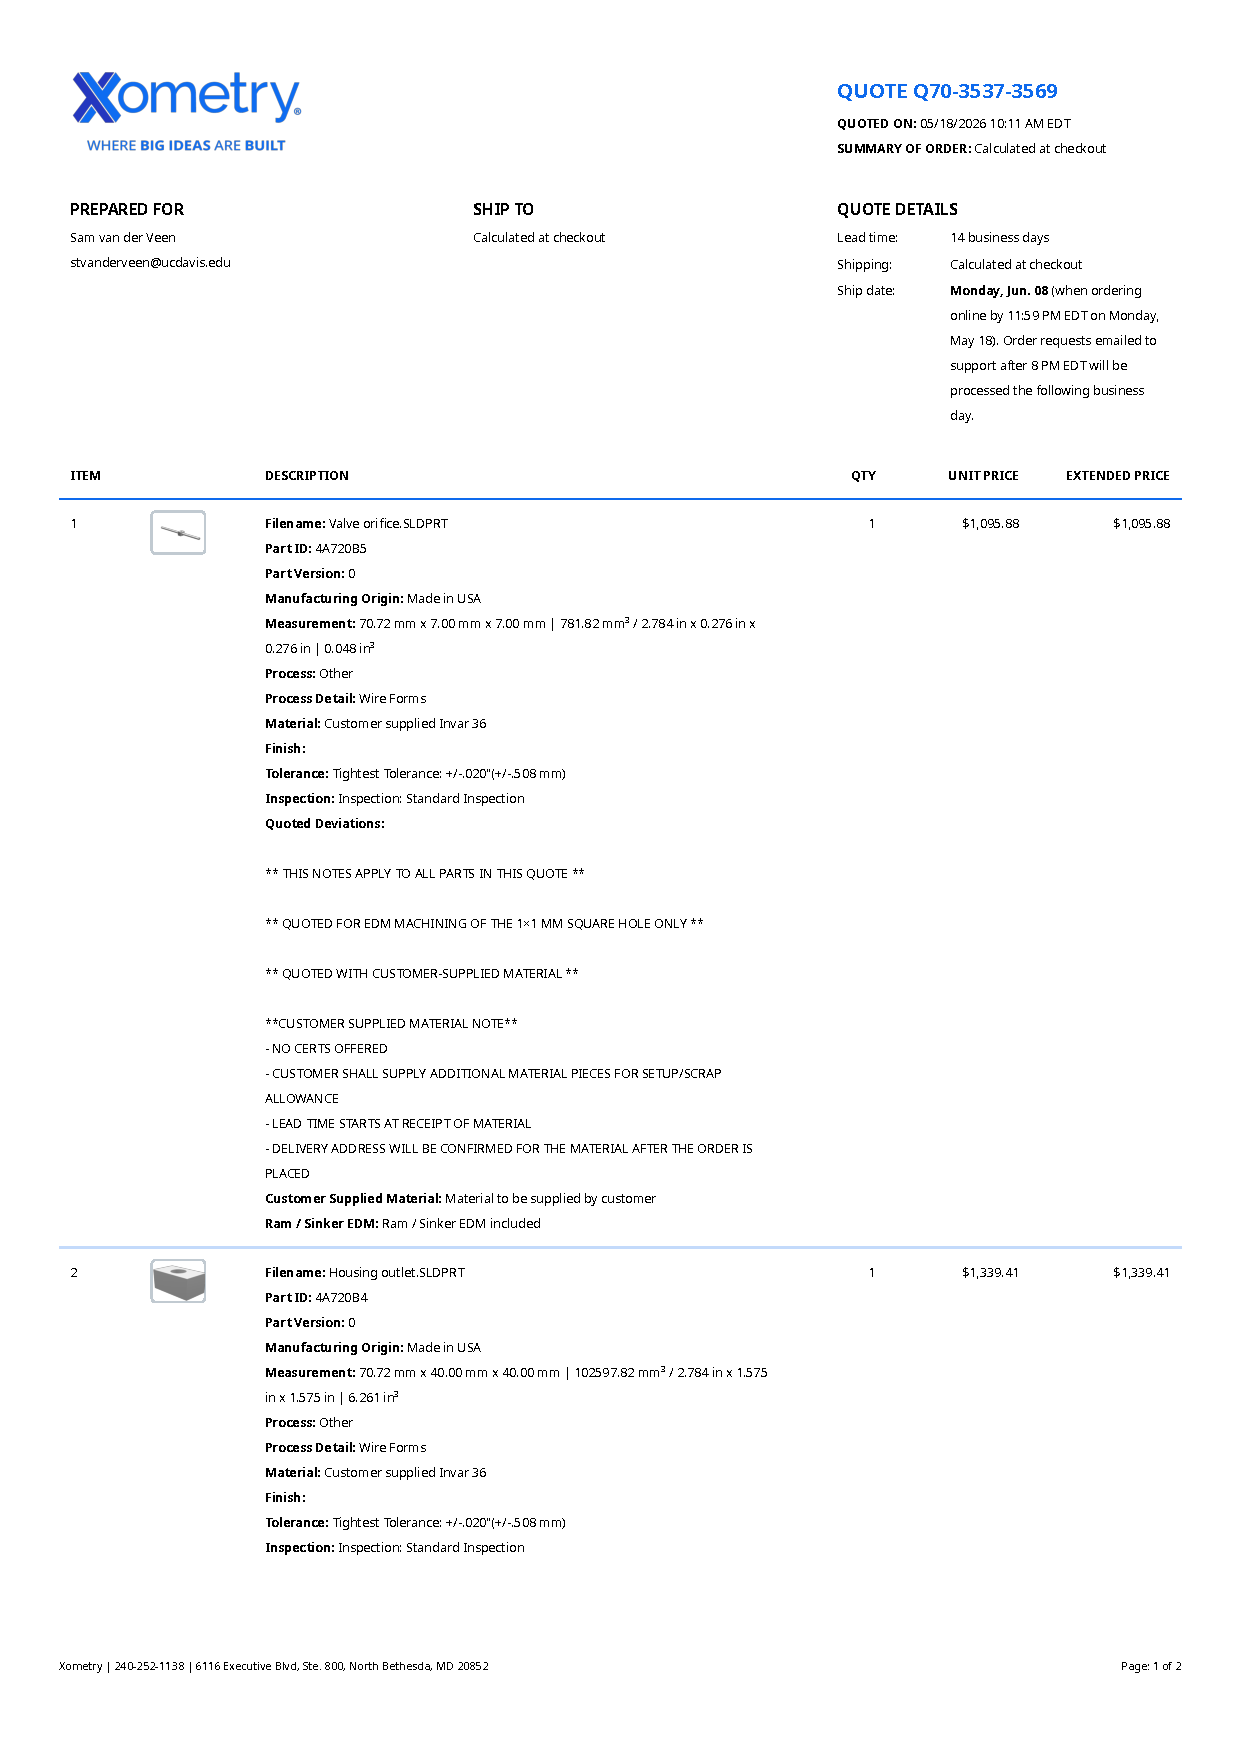
\includepdf[pages=1-2, fitpaper=true, landscape=true]{pdf/quote_EDM.pdf}

\chapter{Manufacturing and Operation}

	\chapter*{Manufacturing Guide}
	\refstepcounter{section}
	\label{app:mfg}
	\addcontentsline{toc}{section}{Manufacturing Guide}
	\addtocontents{toc}{\protect\setcounter{tocdepth}{-1}}
	\setcounter{section}{0}
	\renewcommand{\thesection}{\arabic{section}}

	\begin{center}
		{\Large \textbf{Passive Temperature Compensation Device (PTCD)}} \\[4pt]
		Noble Aggie Labs \\
		Revision 1.0 \\
		June 2026
	\end{center}

	\bigskip

	% ──────────────────────────────────────────────────────────────
	%  SAFETY NOTICES
	% ──────────────────────────────────────────────────────────────

	\begin{warningbox}
		\textbf{\large \textcolor{warnred}{CRITICAL SAFETY NOTICE}}

		\medskip
		Manufacture of this device involves \textbf{sharp tools}, \textbf{high temperatures},
		and dangerous assembly processes such as \textbf{electron-beam welding}.
		Failure to follow these instructions may result in \textbf{serious injury or death.}

		\medskip
		\begin{itemize}[leftmargin=1.5em, itemsep=2pt]
			\item All personnel must be trained in their shop's applicable safety protocols before
						beginning any operation in this guide.
			\item \textbf{Machining:} Sharp cutting tools cause severe lacerations. Never reach into
						a spinning workpiece or move your hands near an unguarded cutter. Wear safety
						glasses at all times on the shop floor. Flying chips are a serious eye hazard.
			\item \textbf{Band saw:} Keep fingers clear of the blade at all times. Use a ``chicken finger''
						to manipulate small stock. Do not force any cut.
			\item \textbf{Heat treatment:} The annealing furnace operates at temperatures up to
						\SI{1040}{\degreeCelsius}. Wear heat-resistant gloves and a face shield when
						loading, unloading, or working near an open furnace.
						Allow parts to cool for at least three hours before handling.
			\item \textbf{Electron-Beam Welding (EBW):} EBW generates high-voltage X-rays and an
						intense electron beam. Only trained and certified EBW operators may perform
						welding operations. The operator must confirm the vacuum chamber is sealed and
						all radiation interlocks are engaged before initiating any weld.
		\end{itemize}
	\end{warningbox}
	\newpage
	\begin{warningbox}
		\begin{itemize}[leftmargin=1.5em, itemsep=2pt]
			\item \textbf{Electrical Discharge Machining (EDM):} Dielectric fluid is a skin and
						eye irritant and a fire hazard. Wear chemical-resistant gloves. Ensure the machine
						is fully de-energized before accessing the work zone. Properly dispose of spent
						dielectric fluid.
			\item \textbf{General:} Do not work alone on any operation. Wear
						appropriate personal protective equipment (PPE) at all times, including safety glasses, closed-toe shoes, 
						and long pants.
						Do not wear loose clothing or jewelry while in the shop.
		\end{itemize}
	\end{warningbox}

	\bigskip

	% ──────────────────────────────────────────────────────────────
	%  SECTION 1  –  INTRODUCTION AND SCOPE
	% ──────────────────────────────────────────────────────────────
	\section{Introduction and Scope}

	This guide details the complete manufacture, assembly, and calibration of the
	Passive Temperature Compensation Device (PTCD), a thermomechanical valve that
	passively adjusts a microscopic orifice in response to ambient air temperature.


	\subsection{Required Tools}

	\begin{notebox}
		\textbf{The following tools and machines are required:}
		\begin{itemize}[itemsep=2pt]
			\item Computer-Numeric Control (CNC) mill and lathe that can meet or exceed the dimensional
						tolerances specified
			\item Band saw
			\item Annealing/heat-treatment furnace capable of reaching \SI{1040}{\degreeCelsius}
			\item Wire EDM (Electrical Discharge Machining) capability
			\item Electron-Beam Welding (EBW) capability
			\item Two perpendicular granite surfaces. One surface must have a drilled hole whose center
						is \SI{20}{\milli\meter} from the intersection between the two surfaces. The
						hole must measure at least \SI{3.4}{\milli\meter} in diameter and \SI{5.1}{\milli\meter}
						depth.
			\item T6 hand screwdriver
		\end{itemize}
	\end{notebox}
	\newpage
	\begin{notebox}
		\begin{itemize}
			\item New, sharp, carbide steel tools of the following types and sizes:
						\begin{itemize}
							\item End mills: 3~mm, 6~mm, 12~mm, and 25~mm
							\item End mill $\geq$\,45~mm length (any diameter)
							\item Drill bits: \nicefrac{1}{8}'', \nicefrac{59}{64}'', \#30, 1.6~mm,
										2.2~mm, 3.5~mm, 16~mm
							\item Reamers: \#29, 18~mm
							\item Lathe inserts: CNMG (roughing) and CCMT (finishing)
							\item Taps: \nicefrac{3}{4}-14~NPT and M2$\times$0.4
						\end{itemize}
			\item Loctite 243 or similar permanent thread sealant
			\item Cutting fluid for all operations
		\end{itemize}
	\end{notebox}

	\subsection{Coordinate System}

	\begin{notebox}
		\textbf{Coordinate convention used throughout this guide:}
		\begin{itemize}[itemsep=2pt]
			\item \textbf{X~(lateral):} points to the right as one looks downstream along the gas flow.
			\item \textbf{Y~(vertical):} points directly upward.
			\item \textbf{Z~(longitudinal):} points upstream along the direction of gas flow.
		\end{itemize}
	\end{notebox}

	These are depicted in Figure~\ref{fig:mfg:axes}.

	\begin{figure}[H]
		\centering
		\includegraphics[width=.5\textwidth]{Axes_mfg.png}
		\caption{Reference axes}
		\label{fig:mfg:axes}
	\end{figure}

	% ──────────────────────────────────────────────────────────────
	%  SECTION 2  –  PART IDENTIFICATION
	% ──────────────────────────────────────────────────────────────
	\section{Part Identification}

	Before beginning, familiarize yourself with every part using Figures \ref{fig:mfg_valve_ID} and \ref{fig:mfg_act_ID}.

	\begin{figure}[H]
		\centering
		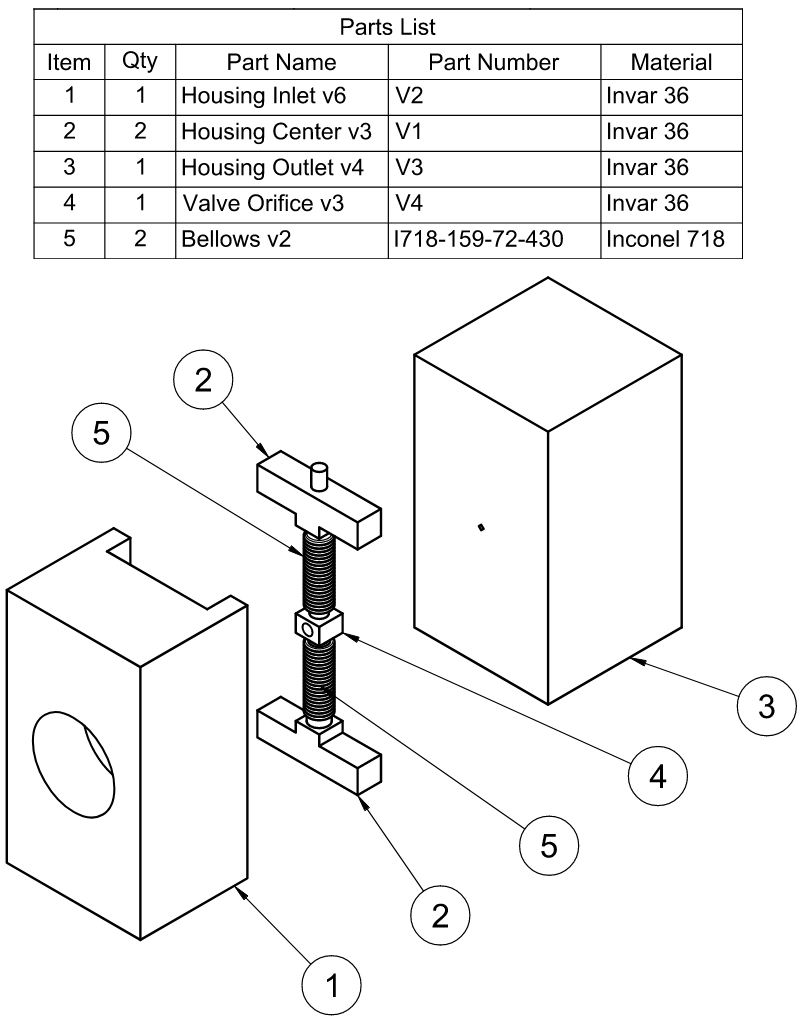
\includegraphics[width=.5\textwidth]{Valve_ID.png}
		\caption{Valve subsystem part identification}
		\label{fig:mfg_valve_ID}
	\end{figure}

	\begin{figure}[H]
		\centering
		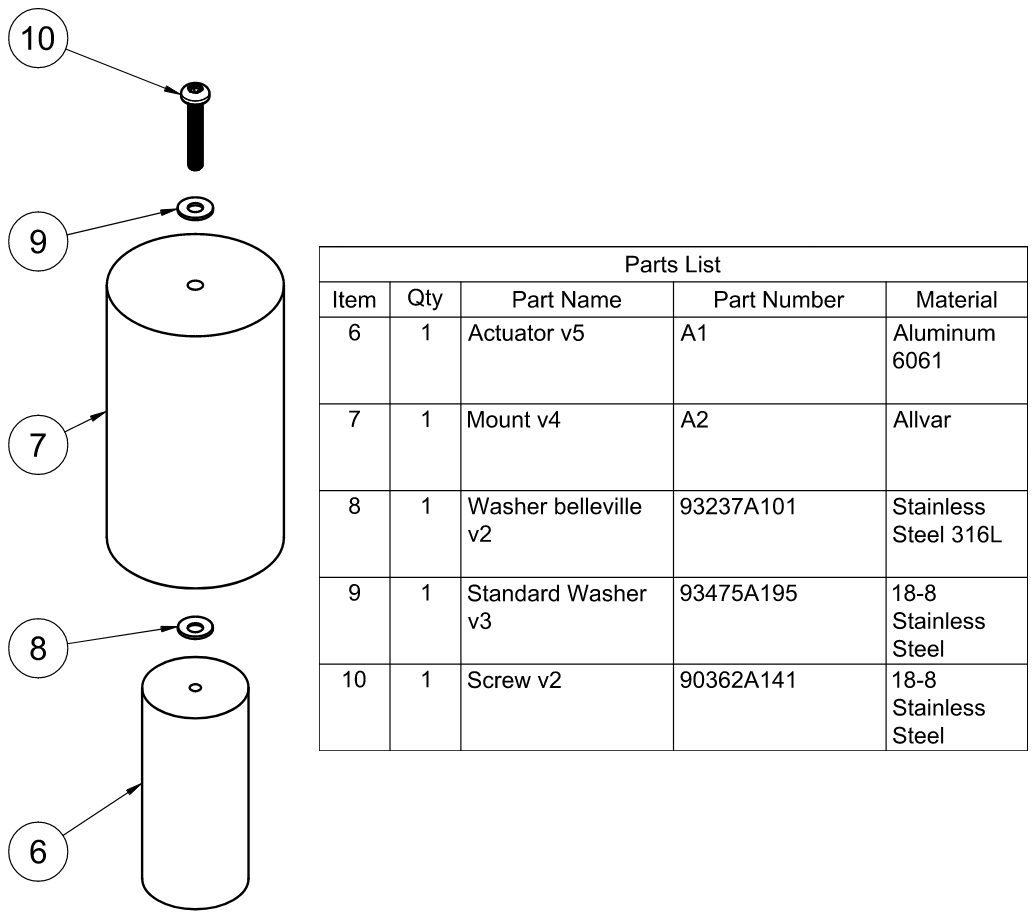
\includegraphics[height=.4\textheight]{Act_ID.png}
		\caption{Actuator subsystem part identification}
		\label{fig:mfg_act_ID}
	\end{figure}

	Table~\ref{tab:mfg_parts} summarises all parts manufactured or purchased for this device.

	\begin{table}[H]
		\centering
		\caption{PTCD Bill of Materials Summary}
		\label{tab:mfg_parts}
		\small
		\begin{tabularx}{\textwidth}{llllX}
			\toprule
			\textbf{Part No.} & \textbf{Name} & \textbf{Qty} & \textbf{Material} & \textbf{Source} \\
			\midrule
			V1 & Housing Center   & 2 & Invar 36    & Machined from billet stock \\
			V2 & Housing Inlet    & 1 & Invar 36    & Machined from billet stock \\
			V3 & Housing Outlet   & 1 & Invar 36    & Machined from billet stock \\
			V4 & Valve Orifice    & 1 & Invar 36    & Machined from billet stock \\
			I718-159-72-430 & Bellows & 2 & Inconel 718 & Purchased (Mini-Flex) \\
			A1 & Actuator         & 1 & Al 6061-T6  & Machined from rod stock \\
			A2 & Mount            & 1 & ALLVAR 30   & Machined from rod stock \\
			93237A101 & Belleville Washer & 1 & 316 SS & Purchased (McMaster-Carr) \\
			93475A195 & Standard Washer   & 1 & 18-8 SS & Purchased (McMaster-Carr) \\
			90362A141 & Screw M2$\times$0.4$\times$12 & 1 & 18-8 SS & Purchased (McMaster-Carr) \\
			\bottomrule
		\end{tabularx}
	\end{table}

	% ──────────────────────────────────────────────────────────────
	%  SECTION 3  –  MANUFACTURING
	% ──────────────────────────────────────────────────────────────
	\section{Manufacturing}
	\label{sec:mfg}

	\subsection{General Machining Notes}
	\label{sec:mfg:general}

	\begin{notebox}
	\textbf{Invar 36 work-hardens during machining.} Use \textbf{new carbide tooling}
	throughout. Replace tooling at the first sign of wear; worn tools exacerbate work
	hardening and degrade surface finish on critical faces.
	\end{notebox}

	\textbf{Annealing schedule for all Invar 36 parts:}
	\begin{enumerate}[itemsep=2pt]
		\item \textbf{Before machining}: anneal at
					\SI{1040}{\degreeCelsius} (\SI{1900}{\degree F}) for 60~minutes to
					reduce as-received hardness and improve machinability\cite[p.~6]{ref_Carpenter_Inv}.
		\item \textbf{After all machining is complete}: anneal at
					\SI{93}{\degreeCelsius} (\SI{200}{\degree F}) for 48~hours to relieve
					residual stress and improve long-term dimensional
					stability\cite[p.~6]{ref_Carpenter_Inv}.
	\end{enumerate}
	Allow parts to air-cool to room temperature before measuring or proceeding to the
	next operation.

	\textbf{Referencing convention:}
	Before beginning each machining operation, identify which face will serve as the
	primary datum. As indicated in the drawings, each of these faces must be carefully
	finished to minimize dimensional errors for critical features.

	% ----------------------------------------------------------
	\subsection{Invar 36 Billet Stock: V1, V2, V3, V4}
	\label{sec:mfg:invar}
	% ----------------------------------------------------------

	\textbf{Starting stock:}
	\SI{44.45}{mm} $\times$ \SI{76.2}{mm} $\times$ \SI{88.9}{mm}
	(1\,\nicefrac{3}{4}$''$ $\times$ 3$''$ $\times$ 3\,\nicefrac{1}{2}$''$) Invar 36 billet.
	These dimensions will be oriented along the \textbf{lateral (X), vertical (Y), and
	longitudinal (Z)} dimensions, respectively.

	\begin{warningbox}
	\textbf{\textcolor{warnred}{WARNING --- Band Saw Hazard}}
	Keep fingers and hands clear of the band saw blade at all times. Use the fence or a
	chicken finger to guide stock. Never reach over or behind the blade during a cut. Allow the
	blade to come to a complete stop before adjusting the workpiece.
	\end{warningbox}

	\subsubsection{Step 1 --- Cross-cut longitudinal axis into blanks}

	Using a metal-cutting band saw, cross-cut the longitudinal axis (Z) to produce blanks
	of the following \textit{minimum} lengths, leaving additional length for subsequent
	facing operations:

	\begin{itemize}[itemsep=2pt]
		\item Housing Inlet (V2): \SI{32}{\milli\meter} 
		\item Housing Outlet (V3): \SI{40}{\milli\meter}
		\item Housing Center (V1) / Valve Orifice (V4): \SI{7}{\milli\meter}
	\end{itemize}

	\begin{notebox}
	Account for the band saw blade kerf thickness when planning cut locations.
	Typical metal band saw kerfs are \SIrange{1}{2}{\milli\meter} wide. Ensure adequate
	additional material remains on each blank after accounting for kerf and facing stock.
	\end{notebox}

	\subsubsection{Step 2 --- Cross-cut lateral axis to separate V1 and V4 slugs}

	Cross-cut the 7~mm slug along the \textbf{lateral axis (X)} to produce:

	\begin{itemize}[itemsep=2pt]
		\item Housing Center $\times$2 (V1): \SI{10}{\milli\meter} lateral length each
		\item Valve Orifice (V4): \SI{7}{\milli\meter} lateral length
	\end{itemize}

	You now have five rough blanks: V2, V3, two pieces of V1, and V4.

	\subsubsection{Step 3 --- Anneal blanks}

	To soften the material before machining the part features,
	place all five blanks in the annealing furnace. Anneal at \SI{1040}{\degreeCelsius} for
	60~minutes. Allow to air-cool to room temperature before proceeding.

	% ------ V1: Housing Center ------
	\subsubsection{Housing Center (V1) --- $\times$2}
	\label{sec:mfg:V1}

	Refer to drawing V1. Produce both Housing Centers identically.

	% \newpage
	\begin{notebox}
	\textbf{Invar 36 tooling} \\
	Use new, sharp, carbide steel tools to machine all features on the Invar 36 parts.
	Invar hardens as it is machined. Cut with slow, shallow passes and ample cutting fluid.
	Replace tools when necessary to ensure precise, consistent dimensions.
	\end{notebox}

	\begin{enumerate}[itemsep=4pt]
		\item \textbf{Mill all six faces} to bring the part to nominal square dimensions
					with 12\,mm end mill.
		\item \textbf{Mill two T-slots on the lateral sides} for the
					valve orifice sliding interface
					with a 12 mm end mill facing from the +X and -X directions, respectively.
		\item \textbf{Drill through-hole} for the valve stem passage
					with a \#30 drill bit from the -Y direction.
					Use a \#29 reamer to bring to final H7 tolerance.
		\item \textbf{Label Housing Inlet} with a stamp on an external face.
	\end{enumerate}

	% ------ V2: Housing Inlet ------
	\subsubsection{Housing Inlet (V2)}
	\label{sec:mfg:V2}

	Refer to drawing V2.

	\begin{enumerate}[itemsep=4pt]
		\item \textbf{Mill all six faces} to nominal rectangular dimensions with a 12 mm end mill.
		\item \textbf{Finishing pass on critical faces}
					(the $+$X and $+$Y faces) with a 12 mm end mill.
					\begin{notebox}
					\textbf{The +X face} is the primary reference for the Housing Inlet.
					Machine this face last among the milled faces, with a dedicated finishing pass
					using a sharp tool at a slow feed rate and light depth of cut.
					The resulting surface must be mirror-smooth; verify with a surface-finish
					gauge or profilometer. This face will be used for critical dimension measurements
					and will be held flush with the corresponding face on the Housing Outlet
					during EBW assembly.
					\end{notebox}
		\item \textbf{Mill top T-groove} with a 6 mm end mill from the +Y direction.
		\item \textbf{Mill bottom T-groove} with a 6 mm end mill from the -Y direction.
		\item \textbf{Mill central channel} through the -Z face with a 6 mm end mill.
		\item \textbf{Drill large central hole} with a \nicefrac{59}{64}'' drill bit.
		\item \textbf{Drill small inlet hole}
					from the -Z direction with an \nicefrac{1}{8}'' drill bit.
		\item \textbf{Tap large hole} with a \nicefrac{3}{4}-14\,NPT (National Pipe Taper) tap. Use cutting fluid.
	\end{enumerate}

	% ------ V3: Housing Outlet ------
	\subsubsection{Housing Outlet (V3)}
	\label{sec:mfg:V3}

	Refer to drawing V3.

	\begin{enumerate}[itemsep=4pt]
		\item \textbf{Mill all six faces} to nominal dimensions with a 12 mm end mill.
		\item \textbf{Finishing pass on Critical Faces A, B, and C}
					(the $+$X, $+$Y, and $+$Z faces respectively) with a 12 mm end mill.
					\begin{notebox}
					\textbf{The +X and +Y faces} are the primary references for the Housing Outlet.
					Machine these faces last among the milled faces, with a dedicated finishing pass
					using a sharp tool at a slow feed rate and light depth of cut.
					The resulting surfaces must be mirror-smooth; verify with a surface-finish
					gauge or profilometer. These faces will be used for critical dimension measurements
					and will be held flush with the corresponding faces on the Housing Inlet
					during EBW assembly. \\
					\textbf{The +Z face} must be similarly finished to ensure even abutment against the Housing Inlet.
					\end{notebox}
		\item \textbf{Drill large central hole} with a \nicefrac{59}{64}'' drill bit.
		\item \textbf{Pre-drill small orifice hole} with a 3.5 mm drill bit. Leave at least 1 mm clearance between the bit tip and the bottom of the cut.
		\item \textbf{Plunge small orifice hole} with a 3 mm end mill. Cut slowly at a shallow angle to avoid breaking the small bit.
					Keep in mind that the workpiece will have hardened after the previous operation.
		\item \textbf{Tap large hole} with a \nicefrac{3}{4}-14\,NPT tap. Use cutting fluid.
		\item \textbf{Wire EDM --- square through-orifice:}
					\begin{warningbox}
					\textbf{\textcolor{warnred}{WARNING --- EDM Hazard}}
					The dielectric fluid used in EDM is a fire hazard and a skin/eye irritant.
					Wear chemical-resistant gloves and eye protection. Ensure the EDM machine is
					fully de-energized before accessing the work zone. Dispose of spent fluid per
					facility hazardous-waste procedures.
					\end{warningbox}
					Machine the square through-orifice using wire EDM.
					Critical requirements:
					\begin{itemize}[itemsep=2pt]
						\item The \textbf{upper interior corner} of the square orifice must have as
									small a fillet radius as possible.
									This is the mission-critical corner; a larger fillet directly degrades
									the effective diameter accuracy.
						\item minimize EDM recast (white) layer on all orifice edges; no
									micro-cracking is permitted.
						\item Thoroughly clean the part after EDM to remove all dielectric fluid
									and microscopic debris before proceeding.
						\item The horizontal and vertical position of the critical
									upper corner must be held as exactly as possible.
									Verify with optical metrology after EDM.
					\end{itemize}
	\end{enumerate}

	\begin{notebox}
	\textbf{EDM Integrity Verification} \\
	Confirmation of the above requirements requires a destructive test.
	Perform an identical operation to the one specified on a sample workpiece. Carefully cut
	the piece in two along its central axis and optically verify that no EDM recast or
	micro-cracking is present.
	\end{notebox}

	% ------ V4: Valve Orifice ------
	\subsubsection{Valve Orifice (V4)}
	\label{sec:mfg:V4}

	Refer to drawing V4.

	\begin{enumerate}[itemsep=4pt]
		\item \textbf{Mill $\pm$Y faces} to bring part to nominal height.
		\item \textbf{Mill $\pm$Z and $\pm$X faces} to bring part to nominal rectangular
					dimensions.
		\item \textbf{Finish all faces} except for the -Y face, paying especial attention
					to the +X face.
		\item \textbf{Mill valve stem}. From several direction perpendicular to the vertical axis,
					cut the corners of the workpiece along the valve stem dimension with a 25 mm end mill
					to bring its shape to a rough cylinder.
					Leave a few mm clearance above and below the rectangular section.
		\item \textbf{Lathe valve stem}. Turn the two shafts to nominal diameter with a CNMG lathe tool.
					Bring to tolerance with a finishing pass using a CCMT lathe tool.
		\item \textbf{Plunge small hole} with an end mill.
		\item \textbf{Wire EDM --- square through-orifice (leading orifice):}
					Machine the square through-orifice using wire EDM as per the above EDM operation.
		\item \textbf{TiCN PVD coating:} Apply a TiCN (titanium carbonitride) Physical Vapor
					Deposition coating to the four contact surfaces per drawing V4, Note~5.
					Confirm the coating thickness does not exceed \SI{0.004}{\milli\meter};
					re-measure the g6 dimensions after coating and verify the fit is maintained
					before proceeding to assembly.
	\end{enumerate}

	% ----------------------------------------------------------
	\subsection{6061 Aluminum Rod Stock: A1 (Actuator)}
	\label{sec:mfg:A1}
	% ----------------------------------------------------------

	\textbf{Starting stock:}
	\O\,\SI{19.05}{\milli\meter} $\times$ \SI{76.2}{\milli\meter}
	(\O\,3/4$''$ $\times$ 3$''$) 6061-T6 Aluminum rod.

	\begin{enumerate}[itemsep=4pt]
		\item \textbf{Band saw --- cut to length:} Cross-cut the rod to a length slightly
					above nominal with a band saw; leave material for facing.
		\item \textbf{Mill to length:} Face both $+$Y and $-$Y ends with a 12 mm to bring the part close to nominal length.
		\item \textbf{Finishing pass on $+$Y face (top):}
					\begin{notebox}
					The length of the actuator is a
					\textbf{critical dimension}: it directly sets the actuator expansion rate.
					Dimension with care.
					\end{notebox}
		\item \textbf{Lathe --- turn outside diameter:} Turn the outer diameter with a CNMG lathe tool.
					Finish to tolerance with a CCMT lathe tool.
		\item \textbf{Drill central hole:} Drill the axial hole
					through the top of the part with a 1.6 mm drill bit, centred on the axis.
					\newpage
					\begin{notebox}
					\textbf{Drill with care}\\
					The 1.6 mm drill bit is small and delicate.
					Apply ample cutting fluid. Peck periodically to remove chips.
					Avoid excessive force to minimize the risk of bit-walking or breakage.
					\end{notebox}
		\item \textbf{Tap:} the hole with an M2$\times$0.4 tap.
	\end{enumerate}

	% ----------------------------------------------------------
	\subsection{ALLVAR 30 Rod Stock: A2 (Mount)}
	\label{sec:mfg:A2}
	% ----------------------------------------------------------

	\textbf{Starting stock:}
	\O\,\SI{25.4}{\milli\meter} $\times$ \SI{45.72}{\milli\meter}
	(\O\,1$''$ $\times$ 1.85$''$) ALLVAR Alloy 30 rod.

	\begin{enumerate}[itemsep=4pt]
		\item \textbf{Band saw --- cut to length:} Cross-cut the rod slightly above
					nominal with a band saw.
		\item \textbf{Mill to length:} Face both ends to remove saw marks and bring to
					near-nominal height with a 12 mm end mill.
		\item \textbf{Turn outer diameter:} turn the outer diameter with a finishing pass with a CCMT lathe tool.
		\item \textbf{Finishing pass on $-$Y face (bottom):} Finish the -Y face with a 12 mm end mill.
					% \newpage
					\begin{notebox}
					The $-$Y face is electron-beam welded to the top of the housing. A flat,
					clean surface is essential for the intimate joint
					required by EBW. Machine this face last with a
					light finishing pass. Verify flatness with a surface plate and feeler gauge
					before proceeding.
					\end{notebox}
		\item \textbf{Drill small clearance hole:} Drill
					the center through hole to a minimum depth of \SI{7}{\milli\meter}
					with a 2.2 mm drill bit.
		\item \textbf{Drill large inner hole:}
					Drill with a 16 mm drill bit. Leave 2--3 mm axial clearance to avoid exceeding the nominal cut depth.
		\item \textbf{Ream large inner hole:}
					Ream the hole to nominal diameter. Leave axial clearance as before.
		\item \textbf{Plunge large inner hole:}
					Plunge the hole with an end mill at least 45 mm long.
					Perform a finishing pass to bring the
					hole's length to tolerance and to square the circumference of its inner face.
	\end{enumerate}

	% ──────────────────────────────────────────────────────────────
	%  SECTION 4  –  ASSEMBLY
	% ──────────────────────────────────────────────────────────────
	\section{Assembly}
	\label{sec:assy}

	\begin{warningbox}
	\textbf{\textcolor{warnred}{WARNING --- Electron-Beam Welding (EBW) Hazard}}

	EBW generates high-voltage X-ray radiation and a focused electron beam.
	\textbf{Only trained, certified EBW operators} may perform these operations.
	Confirm all radiation interlocks are active and the vacuum chamber is sealed
	before initiating any weld. No EBW operation may be performed by untrained
	personnel under any circumstances.
	\end{warningbox}

	\subsection{General Assembly Notes}

	All permanent joints in the PTCD, except the actuator-mount connection
	secured by the calibration screw,
	are made by Electron-Beam Welding (EBW).
	EBW requirements (drawing W1, W2 notes) apply to all weld operations:

	\begin{enumerate}[itemsep=3pt]
		\item Welding process: EBW (autogenous; no filler metal).
		\item Mating surfaces must be intimate; maximum gap $\leq$\,\SI{0.01}{\milli\meter}.
		\item All surfaces to be welded must be thoroughly cleaned and free of oil, grease,
					and oxidation prior to welding. Use appropriate solvent and clean-room wipes.
		\item Purge internal cavities with inert gas during welding to
					prevent oxidation and spatter.
		\item All wetted EBW joints must be subjected to 100\% X-ray radiographic
					examination to confirm a weld joint efficiency $E = 1.0$ per
					ASME~B31.3\cite{ref_asme_b313}.
	\end{enumerate}

	EBW requires an unobstructed line of sight to the weld joint throughout the
	full rotation of the workpiece. Plan each setup carefully. The sub-assembly
	sequence in Sections~\ref{sec:valve_assy} and~\ref{sec:act_assy} is designed
	to maintain 360$^{\circ}$ weld access at every stage.

	% \newpage
	% ----------------------------------------------------------
	\subsection{Valve Sub-Assembly}
	\label{sec:valve_assy}
	% ----------------------------------------------------------

	\begin{notebox}
	\textbf{Required tooling for valve assembly:}
	\begin{itemize}[itemsep=2pt]
		\item Two perpendicular granite surface plates. One plate must contain a clearance
					hole at least \SI{3.4}{\milli\meter} in diameter and at least \SI{5}{\milli\meter}
					deep at precisely \SI{20}{\milli\meter} from the intersection between the plates
					(to accept the lower valve stem during
					step~\ref{step:lay_granite}).
		\item Clean lint-free gloves and wipes.
		\item Optical comparator or profilometer for verifying face flush and orifice position.
	\end{itemize}
	\end{notebox}

	\begin{figure}[h]
		\centering
		% 
\includegraphics[width=.5\textwidth]{Valve_exploded.png}
		\includegraphics[width=.5\textwidth]{Valve_exploded_qual.png}
		\caption{Valve subsystem exploded view}
		\label{fig:mfg_valve_exploded}
	\end{figure}

	Refer to Figure~\ref{fig:mfg_valve_exploded} and \ref{fig:mfg_valve_ID}.

	\subsubsection{Step 1 --- Weld bellows to Valve Orifice (V4)}

	\begin{enumerate}[itemsep=4pt]
		\item Orient the first (upper) bellows with its \textbf{small neck (Neck~1) toward
					the center} of the Valve Orifice. Seat it on the upper valve stem stub of V4.
		\item Orient the second (lower) bellows identically: small neck toward center, seated
					on the lower valve stem stub.
		\item EBW both bellows to V4 with circumferential welds.
	\end{enumerate}

	\subsubsection{Step 2 --- Add Housing Centers (V1) to valve stems}
	\label{step:add_V1}

	\begin{enumerate}[itemsep=4pt]
		\item Slide one Housing Center (V1) onto the upper valve stem of the
					V4--bellows sub-assembly through its bore.
					The V1 piece should slide freely without binding.
		\item Slide the second Housing Center onto the lower valve stem.
	\end{enumerate}

	\subsubsection{Step 3 --- Lay sub-assembly on granite surface and tack-weld}
	\label{step:lay_granite}

	\begin{enumerate}[itemsep=4pt]
		\item Set the sub-assembly on the
					granite surface plate, with the -Z face against the surface.
		\item Apply \textbf{two spot welds} at each bellows--Housing Center connection 
					to fix their position.
	\end{enumerate}

	\subsubsection{Step 4 --- Full weld of Housing Centers to bellows}

	\begin{enumerate}[itemsep=4pt]
		\item Remove the sub-assembly from the granite surface.
		\item Fully EBW each Housing Center to its bellows with a circumferential weld.
	\end{enumerate}

	\subsubsection{Step 5 --- Insert valve sub-assembly into Housing Inlet (V2)}

	\begin{enumerate}[itemsep=4pt]
		\item Verify that the V4 coated surfaces are clean and the housing channel in V2 is
					free of debris.
		\item Slide the sub-assembly (V4 + bellows + V1~$\times$2) into the central
					channel of the Housing Inlet (V2).
	\end{enumerate}

	\subsubsection{Step 6 --- EBW Housing Centers to Housing Inlet; verify face flush}

	\begin{enumerate}[itemsep=4pt]
		\item With the sub-assembly fully seated in V2, EBW the Housing Centers (V1) to
					the Housing Inlet (V2).
	\end{enumerate}

	\subsubsection{Step 7 --- Finish the Housing Inlet face}

	\begin{enumerate}[itemsep=4pt]
		\item Make a finishing pass across the whole -Z face of the subassembly to
					ensure flush abutment against the Housing Outlet.
					Be careful not to damage the bellows while cutting.
	\end{enumerate}

	\subsubsection{Step 8 --- Connect the Housing Outlet}

	\begin{enumerate}[itemsep=4pt]
		\item Invert the assembly and set its +Y and +X faces flush against the two granite surfaces.
					Use the provided hole to make room for the protruding valve stem.
		\item Set the Housing Inlet in like manner against the granite surfaces.
					Butt its +Z face against the assembly's -Z face.
		\item Weld the assembly along its exposed edges enough to secure the parts in place.
					Remove from the granite surfaces; fully weld the connection.
	\end{enumerate}

	\subsubsection{Step 9 --- Finish the Upper Surface}

	\begin{enumerate}[itemsep=4pt]
		\item Perform a finishing pass on the +Y surface of the assembly.
		Maintain clearance around the valve stem at a minimum of \SI{1}{\milli\meter}
		to avoid damage and a maximum of \SI{7}{\milli\meter} to ensure the full mount-housing
		contact surface is finished.
	\end{enumerate}

	% ----------------------------------------------------------
	\subsection{Actuator Sub-Assembly}
	\label{sec:act_assy}
	% ----------------------------------------------------------

	\begin{figure}[H]
		\centering
		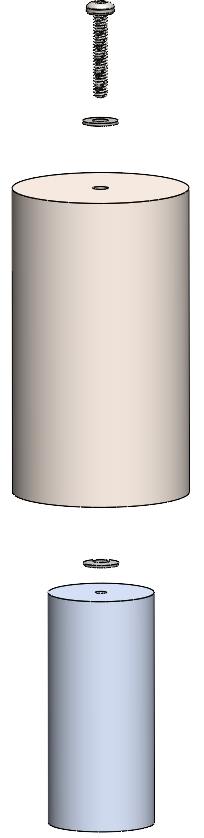
\includegraphics[height=3in]{Act_exploded.png}
		\caption{Actuator subsystem exploded view}
		\label{fig:mfg_act_exploded}
	\end{figure}

	\subsubsection{Step 1 --- EBW Actuator (A1) to upper valve stem}

	\begin{enumerate}[itemsep=4pt]
		\item EBW the actuator to the valve stem.
					Confirm the actuator and valve stem are axially
					aligned; any tilt introduces an off-axis load on the orifice.
	\end{enumerate}

	% \newpage
	\begin{notebox}
	\textbf{Thermal equilibration}\\
	Before proceeding, allow all parts to thermally equilibrate with their environment for a full
	60 minutes. This ensures that the device can be calibrated before the thread lubricant sets.
	\end{notebox}

	\subsubsection{Step 2 --- Add Mount and Calibration Assembly}

	\begin{enumerate}[itemsep=4pt]
		\item Apply Loctite 243 or a similar lubricant-sealant to the screw.
		\item Invert the mount (A2). Insert the screw (90362A141) through the
					standard flat washer (93475A195) and mount.
					Slide the belleville washer (93237A101) onto the screw,
					conical side facing toward the mount top when righted.
		\item Invert the housing-actuator assembly. Carefully insert the actuator into the
					the mount until it hits the screw. Thread the screw into the actuator until the mount
					can sit flush against the housing and the belleville washer is slightly compressed.
		\item Right the assembly and EBW the mount to the housing.
	\end{enumerate}

	\begin{notebox}
	\textbf{Time-sensitive calibration}
	Perform the calibration steps detailed in Section~\ref{sec:calibration} immediately
	to ensure the thread sealant does not set.
	\end{notebox}

	% ──────────────────────────────────────────────────────────────
	%  SECTION 5  –  CALIBRATION
	% ──────────────────────────────────────────────────────────────
	\section{Calibration}
	\label{sec:calibration}

	Calibrate the \device\ at approximately $T_{ref} = \Tref$ (room temperature).

	\subsubsection{Calibration Procedure}

	\begin{enumerate}[itemsep=5pt]
		\item \textbf{Thread the gas supply.} Connect the PTCD to a controlled gas flow
					supply via its threaded interfaces. Precisely measure the ambient temperature
					and the pressure differential across the device.
		\item \textbf{Calculate required pressure drop.} Use the following equations to determine
					the required pressure differential for the current temperature:
					\begin{align}
						D_{\text{effective}} = A_1 (T_{\text{ambient}} - T_{\text{reference}}) + A_0 \\
						A_1 = \Aone \\
						T_{\text{reference}} = \SI{25}{\degreeCelsius} \\
						A_0 = \Azero \\
						A = \frac{\pi}{4} D_{\text{effective}}^2 \\
						Q = C_d A \sqrt{\frac{2 \Delta P}{\rho (1 - \beta^4)}} \label{eq:white}
					\end{align}
					Refer to White's Fluid Mechanics\cite[eq.~6-102]{ref_white} for interpretation of
					equation~\eqref{eq:white}.
		\item \textbf{Adjust the orifice.} Using a T6 Torx driver, turn the calibration
					screw in small increments. Turn it clockwise to increase the effective
					diameter and decrease the pressure differential.
		\item \textbf{Depressurize and disconnect.} Let the system run at steady-state for six hours
					to allow the sealant to fully set under these conditions. Then close the supply valve and vent
					the downstream line before disconnecting any fittings.
	\end{enumerate}

	\setcounter{section}{1}
	\addtocontents{toc}{\protect\setcounter{tocdepth}{3}}
	\renewcommand{\thesection}{\thechapter.\arabic{section}}

	\chapter*{User Guide}
	\refstepcounter{section}
	\label{app:op}
	\addcontentsline{toc}{section}{User Guide}
	\addtocontents{toc}{\protect\setcounter{tocdepth}{-1}}
	\setcounter{section}{0}
	\renewcommand{\thesection}{\arabic{section}}


	\begin{center}
		{\Large \textbf{Passive Temperature Compensation Device (PTCD)}} \\[4pt]
		Noble Aggie Labs \\
		Revision 1.0 \\
		June 2026
	\end{center}

	\bigskip

	\begin{warningbox}
	\textbf{\large \textcolor{warnred}{CRITICAL SAFETY NOTICE}}

	\medskip
	This device operates with \textbf{high-pressure gas up to \SI{68.95}{\mega\pascal} (\num{10000}~psi)},
	including potentially \textbf{flammable gases such as hydrogen.}
	Failure to follow these instructions may result in \textbf{serious injury or death.}

	\medskip
	\begin{itemize}[leftmargin=1.5em, itemsep=2pt]
		\item All personnel must be trained in high-pressure gas handling before working with this device.
		\item All connections and testing must comply with \textbf{ASME~B31.3} and applicable local safety regulations.
		\item Hydrogen is extremely flammable. Work in a well-ventilated area with appropriate gas detection equipment active.
		\item \textbf{Never work on a pressurized system.} Confirm the system is fully depressurized before installation, removal, or adjustment.
		\item Wear appropriate PPE at all times: safety glasses, face shield, and flame-resistant clothing. Use insulated gloves near temperature extremes (\SI{-60}{\degreeCelsius} to \SI{+80}{\degreeCelsius}).
	\end{itemize}
	\end{warningbox}

	\bigskip

	%-------------------------------------------------------------------
	\section{Product Overview}
	%-------------------------------------------------------------------

	\subsection{Background}

	The PTCD is designed for use in high-pressure gas experiments in a controlled laboratory setting. The device is intended to regulate flow of noble gases and hydrogen using passive thermal expansion given ambient temperature differences, and is rated for pressures up to \SI{68.95}{\mega\pascal} (\num{10000}~psi). It is not intended for use with liquids, corrosive gases, or in environments with significant vibration or shock. The PTCD mantains it's specified orifice diameter across a temperature range of \SI{-60}{\degreeCelsius} to \SI{+80}{\degreeCelsius}, and is calibrated at room temperature (\SI{25}{\degreeCelsius}) with the option for field adjustment. It connects to standard gas plumbing with threaded ports and once installed requires no user input or power to operate.

	\subsection{Intended Users}

	This guide is written for test engineers and laboratory technicians who operate high-pressure gas experiments and are familiar with pressurized gas systems and applicable codes. 

	%-------------------------------------------------------------------
	\section{System Description}
	%-------------------------------------------------------------------

	The PTCD has two sub-assemblies. The Valve Sub-assembly is the pressurized body: an Invar 36 housing with threaded pipe ports, an internal sliding Invar~36 orifice plate, and a welded metal bellows that seals the stem while allowing it to move. The Actuator Sub-assembly sits on top. It is a bimetallic cylinder with aluminum on the inside and Allvar on the outside. Because aluminum expands and Allvar contracts when heated, the two materials work together to amplify the net downward displacement transmitted to the valve stem. The actuator is fully isolated from the hot pressurized gas inside the valve.

	\begin{figure}[h]
		\centering
		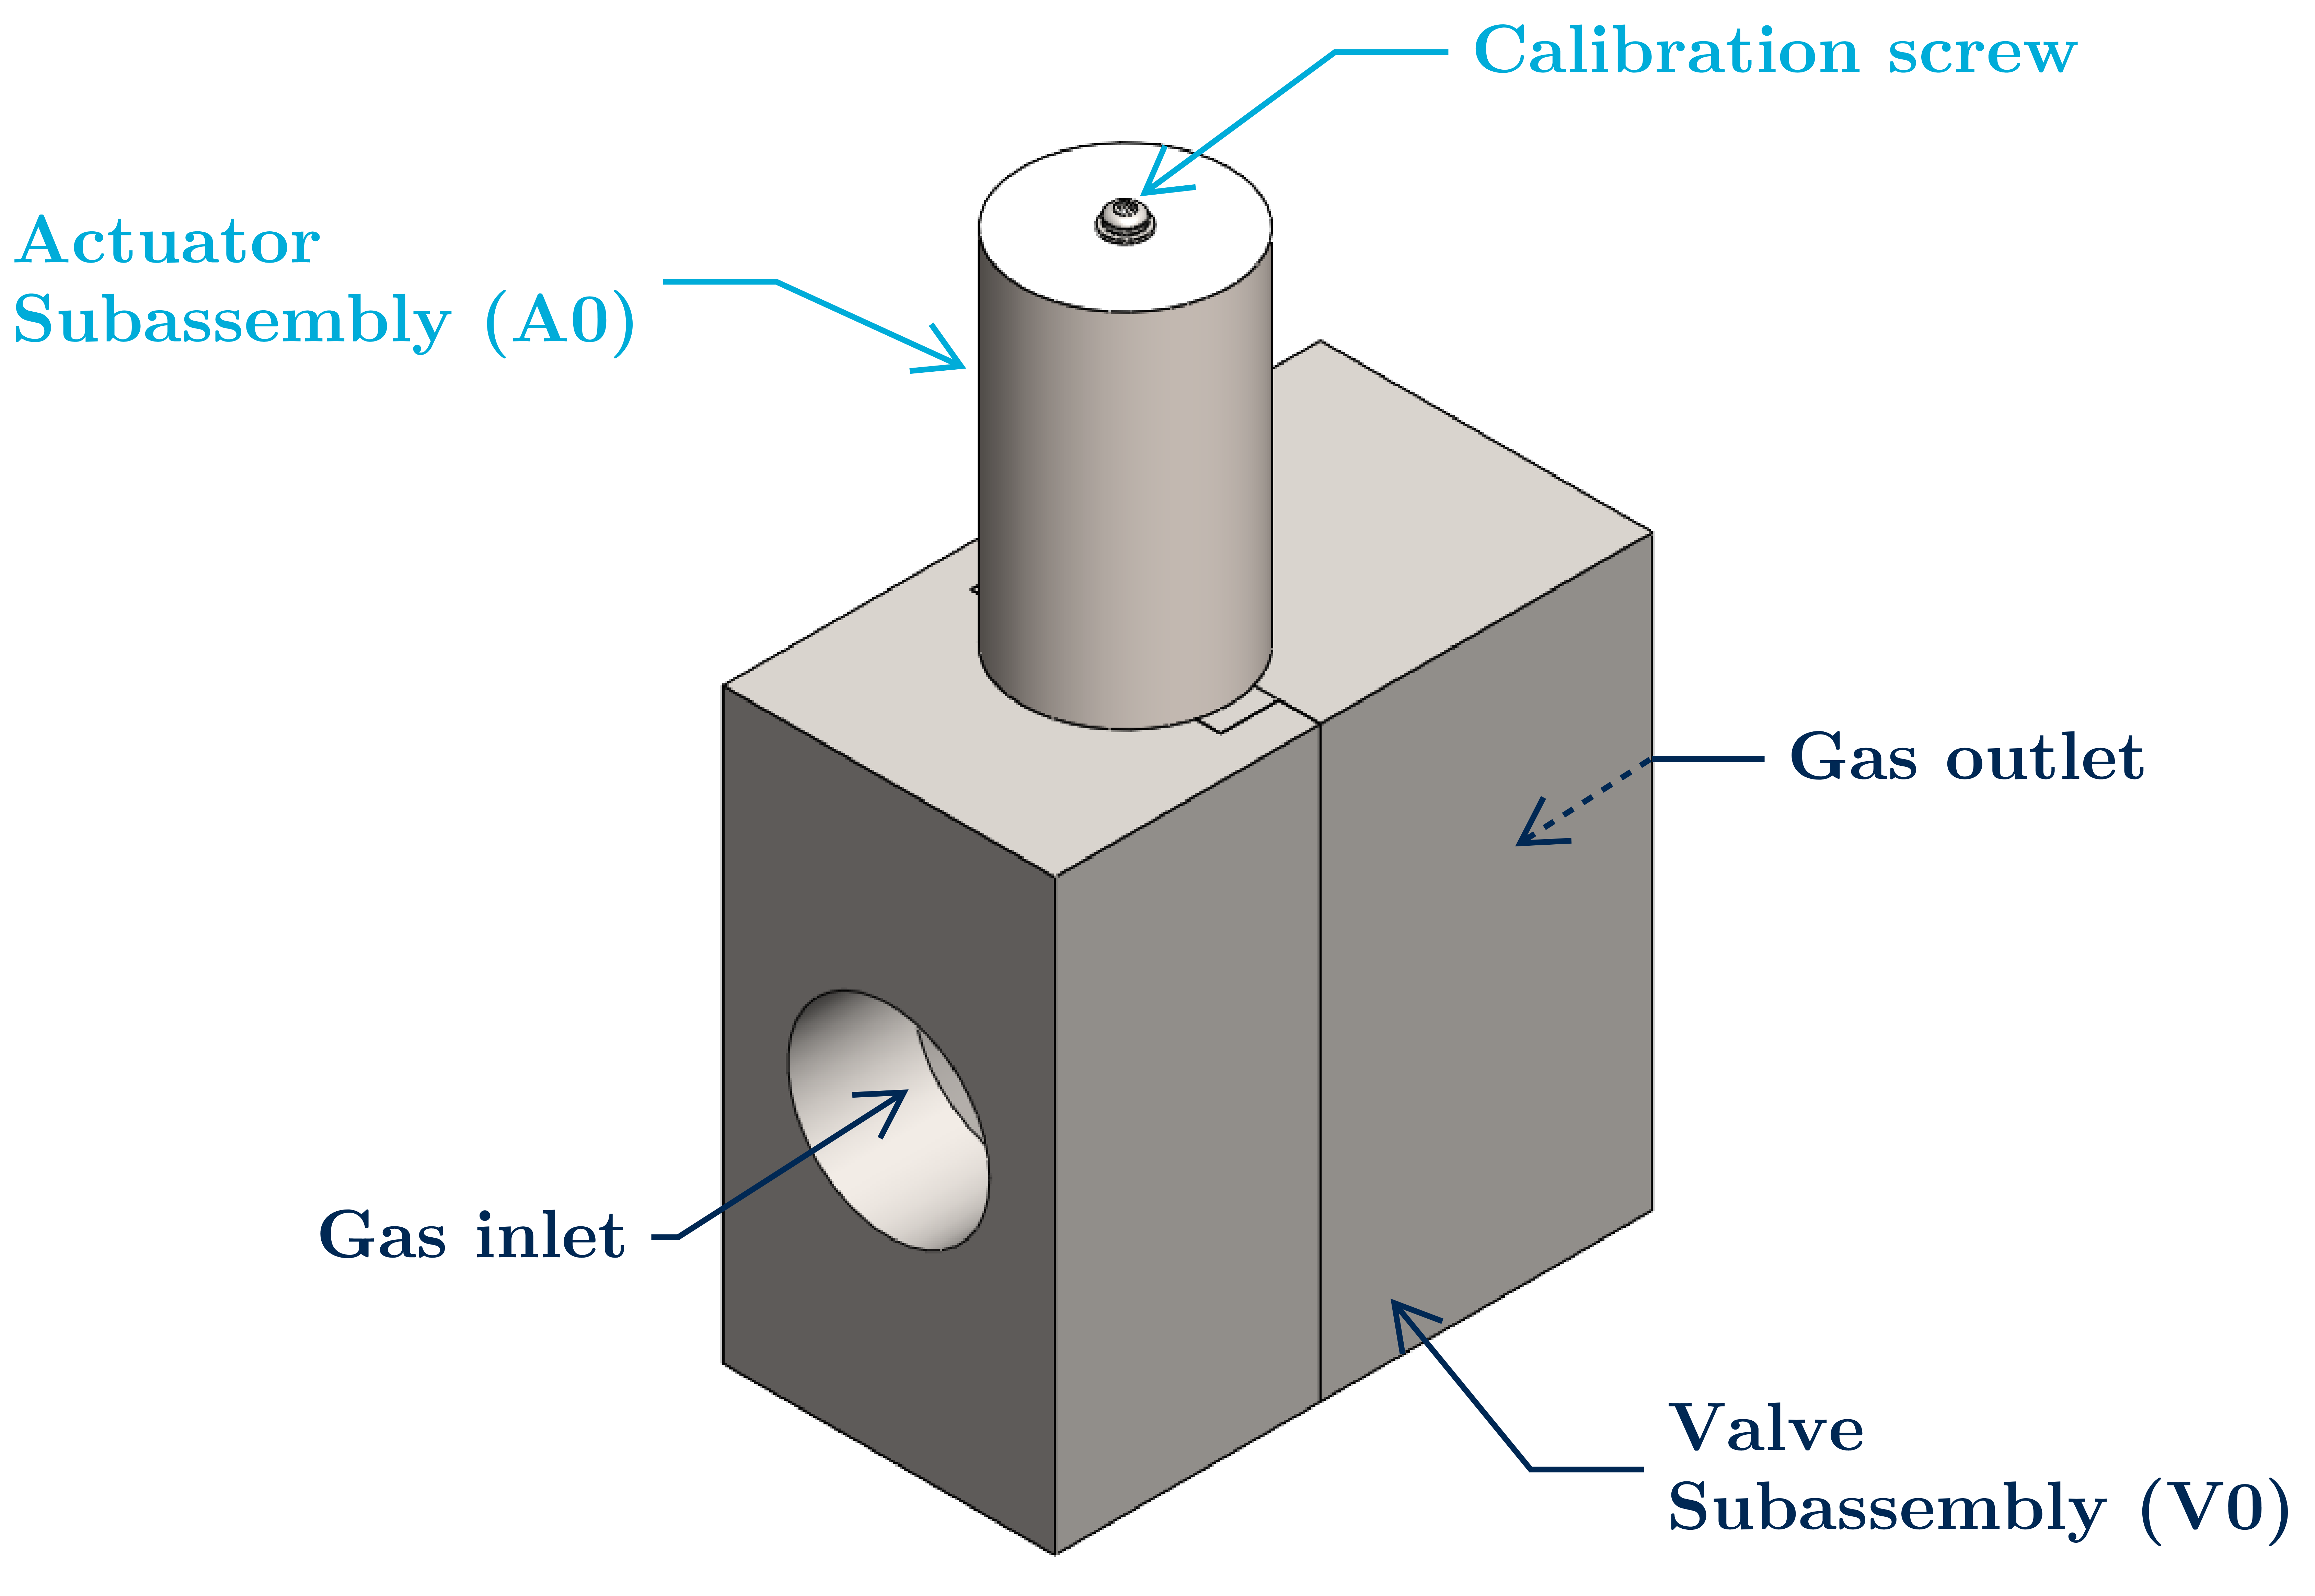
\includegraphics[width=.9\textwidth]{user_isometric.png}
		\caption{Complete PTCD assembly}
		\label{fig:ug_overview}
	\end{figure}

	The PTCD has two sub-assemblies. The Valve Sub-assembly is the pressurised body: an Invar 36 housing with threaded pipe ports, an internal sliding Invar~36 orifice plate, and a welded metal bellows that seals the stem while allowing it to move. The Actuator Sub-assembly sits on top. It is a bimetallic cylinder with aluminum on the inside and Allvar on the outside. Because aluminum expands and Allvar contracts when heated, the two materials work together to amplify the net downward displacement transmitted to the valve stem. The actuator is fully isolated from the hot pressurised gas inside the valve.

	\begin{figure}[h]
		\centering
		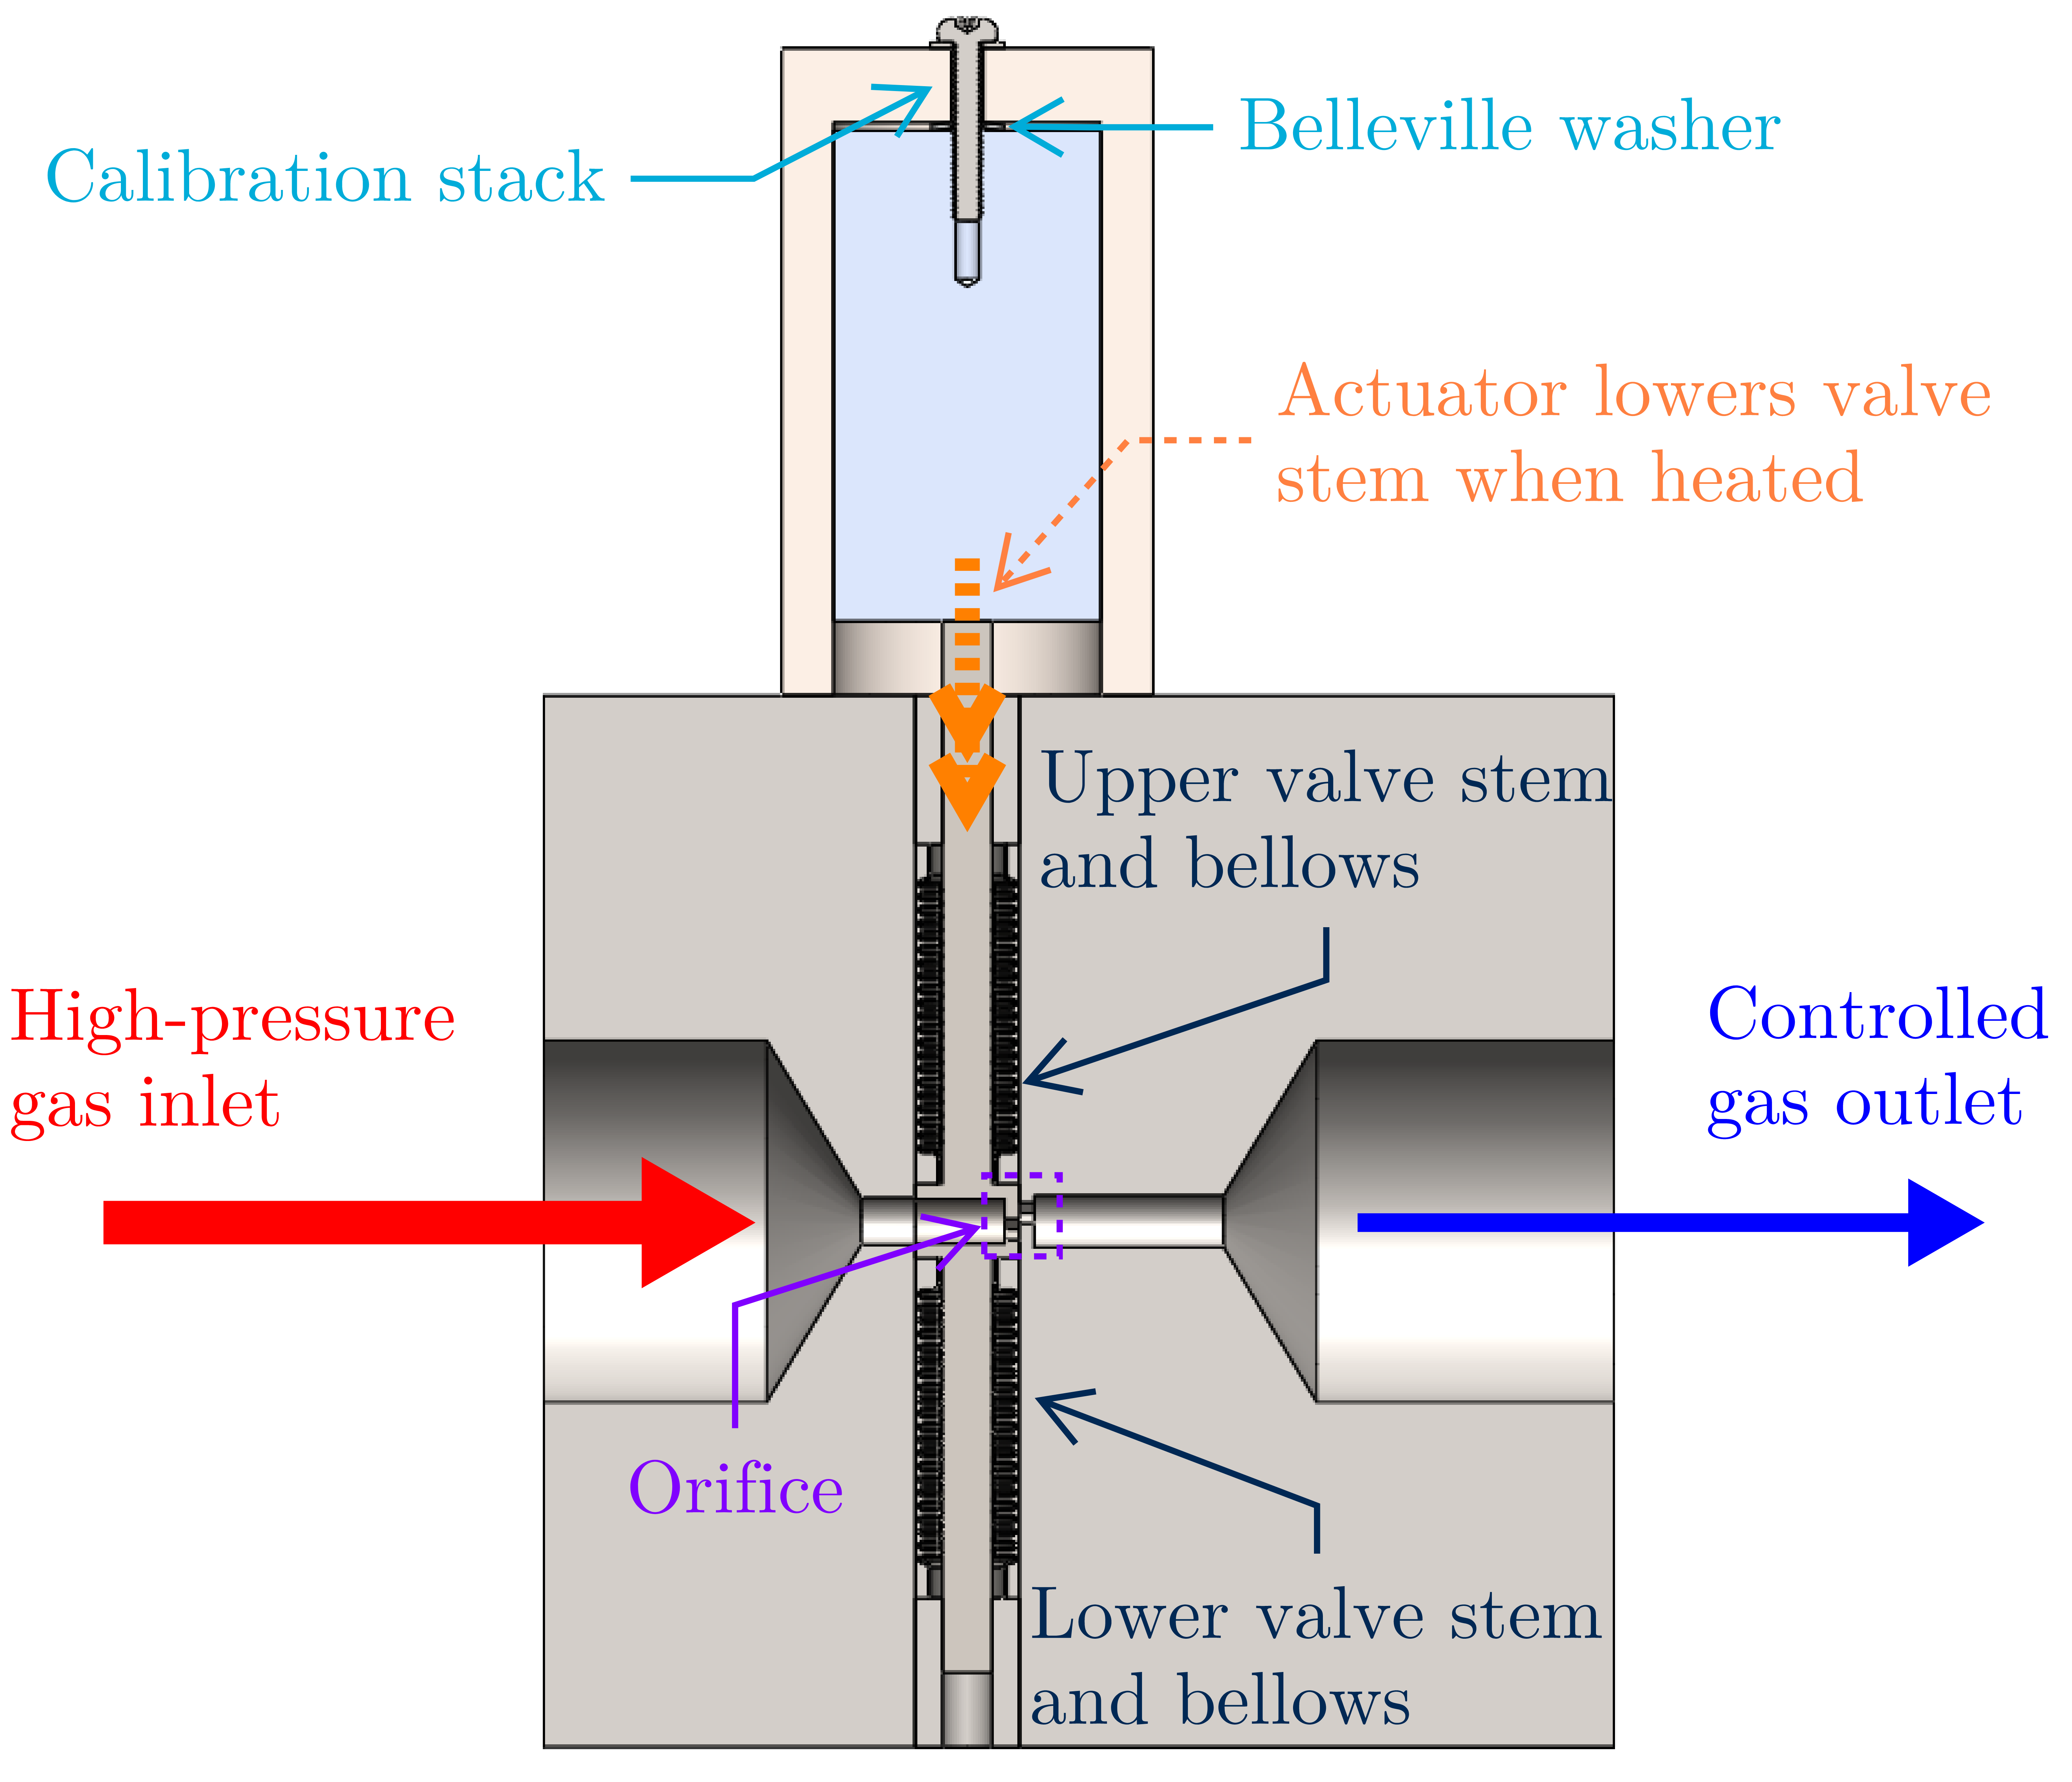
\includegraphics[width=.75\textwidth]{user_cut.png}
		\caption{PTCD cross-section schematic.}
		\label{fig:ug_crosssection}
	\end{figure}


	\textbf{How it works:} Rising ambient temperature causes the actuator to push the valve stem downward, reducing the orifice overlap and restricting flow. Falling temperature pulls the stem back up, opening the orifice. The device requires no power and makes no adjustments on its own --- it simply follows temperature.
	Refer to Figure~\ref{fig:ug_overview} and \ref{fig:ug_crosssection}.


	%-------------------------------------------------------------------
	\section{Before You Begin}
	%-------------------------------------------------------------------

	\subsection{What You Will Need}

	\begin{itemize}[itemsep=3pt]
		\item High-pressure gas supply with upstream shut-off valve and regulator
		\item Compatible pipe with appropriate thread to match the PTCD ports
		\item Pipe sealant approved for the gas and pressure in use (see Section~\ref{sec:sealing})
		\item Two wrenches sized for the pipe fittings
		\item Calibrated pressure gauge (upstream of PTCD)
		\item Hydrogen-rated leak detector or electronic gas sensor
		\item Downstream isolation valve
		\item Rigid, level mounting surface (see Section~\ref{sec:mounting})
		\item PPE: safety glasses, face shield, flame-resistant clothing, insulated gloves
	\end{itemize}

	% \newpage
	\subsection{Pipe Sealing}
	\label{sec:sealing}

	\begin{warningbox}
	\textbf{\textcolor{warnred}{WARNING --- Sealing Requirements}}

	Standard PTFE tape is \emph{not} rated for hydrogen service at pressures above approximately \SI{20}{\mega\pascal}. \textbf{Select a sealing method rated for the full operating pressure and verified compatible with your gas.} Consult ASME~B31.3 and your facility's safety officer before making connections.
	\end{warningbox}

	\subsection{Mounting}
	\label{sec:mounting}
	\textbf{NOTE:} The actuator responds to the temperature of the air surrounding it. Anything that heats or cools the actuator other than the ambient air will introduce error in the orifice diameter.

Mount the PTCD on a rigid, level surface. The actuator must be vertical and tilting the device introduces an unintended gravitational load on the valve stem. Do not mount on a surface that is independently heated or cooled. Keep at least \SI{15}{\centi\meter} of free air clearance around the actuator on all sides, and make sure no cables, clamps, or insulation contact it. Secure the device firmly enough that it will not move under pipe reaction loads once the system is pressurized.

	\subsection{Ambient Air Conditions}

	The device is designed for quasi-static temperature changes. Avoid directing compressed air, fans, or air-conditioning flow at the actuator, as localized forced convection will cause uneven heating and introduce measurement error. Keep the actuator clear of heat lamps and radiant sources. After placing the device in a new temperature environment, allow at least \textbf{60 minutes} for it to equilibrate before pressurising or recording data. Fast temperature changes may cause a transient lag between the ambient reading and the actual orifice position.

	%-------------------------------------------------------------------
	\section{Installation}
	%-------------------------------------------------------------------

	\begin{warningbox}
	\textbf{\textcolor{warnred}{WARNING}} \quad Confirm the upstream supply is \textbf{fully shut off and depressurized} before beginning. Never connect or disconnect the PTCD under pressure.
	\end{warningbox}

	\begin{figure}[htbp]
		\centering
		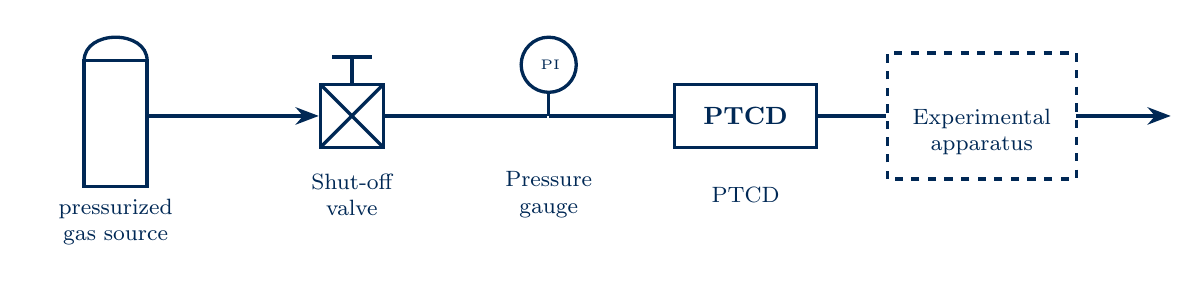
\begin{tikzpicture}[
			>=Stealth,
			line width=0.6pt,
			font=\small,
			pipe/.style={draw, line width=1.2pt, color=ucdblue},
			lbl/.style={text centered, font=\footnotesize, color=ucdblue}
		]

		\def\pipeY{0}
		\def\xSource{0}
		\def\xValve{3}
		\def\xGauge{5.5}
		\def\xPTCD{8}
		\def\xApparatus{11}

		%% 1. Gas cylinder symbol
		\draw[pipe] (\xSource-0.4, \pipeY-0.9) rectangle (\xSource+0.4, \pipeY+0.7);
		\draw[pipe]
			(\xSource-0.4, \pipeY+0.7)
			.. controls (\xSource-0.4,\pipeY+1.1) and (\xSource+0.4,\pipeY+1.1) ..
			(\xSource+0.4, \pipeY+0.7);
		\draw[pipe] (\xSource+0.4, \pipeY) -- (\xSource+0.8, \pipeY);

		\node[lbl, text width=2cm] at (\xSource, \pipeY-1.35)
			{pressurized\\gas source};

		%% Inlet flow arrow
		\draw[->, line width=1.2pt, color=ucdblue] (\xSource+0.8, \pipeY) -- (\xValve-0.42, \pipeY);
		% \node[font=\tiny, above] at (\xSource+1.55, \pipeY+0.08) {flow};

		%% 2. Shut-off valve (ISO 1219: square with X and T-bar actuator)
		\def\vs{0.4}
		\draw[pipe] (\xValve-\vs,\pipeY-\vs) rectangle (\xValve+\vs,\pipeY+\vs);
		\draw[pipe] (\xValve-\vs,\pipeY-\vs) -- (\xValve+\vs,\pipeY+\vs);
		\draw[pipe] (\xValve-\vs,\pipeY+\vs) -- (\xValve+\vs,\pipeY-\vs);
		\draw[pipe] (\xValve,\pipeY+\vs) -- (\xValve,\pipeY+\vs+0.35);
		\draw[pipe] (\xValve-0.25,\pipeY+\vs+0.35) -- (\xValve+0.25,\pipeY+\vs+0.35);
		\draw[pipe] (\xValve+\vs,\pipeY) -- (\xGauge-0.02,\pipeY);

		\node[lbl, text width=2cm] at (\xValve, \pipeY-1.0)
			{Shut-off\\valve};

		%% 3. Pressure gauge (ISA 5.1: circle, needle, tagged PI; branch from pipe)
		\def\gr{0.35}
		\draw[pipe] (\xGauge,\pipeY) -- (\xGauge,\pipeY+0.3);
		\draw[pipe] (\xGauge,\pipeY+\gr+0.3) circle (\gr);
		% \draw[pipe] (\xGauge,\pipeY+\gr+0.3) -- ++(50:\gr*0.7);
		\node[font=\tiny, color=ucdblue] at (\xGauge,\pipeY+\gr+0.3) {\,PI};
		\draw[pipe] (\xGauge,\pipeY) -- (\xPTCD-0.92,\pipeY);

		\node[lbl, text width=2.2cm] at (\xGauge, \pipeY-1.0)
			{Pressure\\gauge};

		%% 4. PTCD (labelled rectangle)
		\def\pw{0.9}
		\def\ph{0.4}
		\draw[pipe] (\xPTCD-\pw,\pipeY-\ph) rectangle (\xPTCD+\pw,\pipeY+\ph);
		\node[font=\small\bfseries, color=ucdblue] at (\xPTCD,\pipeY) {PTCD};
		\draw[pipe] (\xPTCD+\pw,\pipeY) -- (\xApparatus-1.22,\pipeY);

		\node[lbl, text width=2cm] at (\xPTCD, \pipeY-1.0)
			{PTCD};

		%% 5. Experimental apparatus (dashed boundary box)
		\def\aw{1.2}
		\def\ah{0.8}
		\draw[pipe, dashed]
			(\xApparatus-\aw,\pipeY-\ah) rectangle (\xApparatus+\aw,\pipeY+\ah);
		\node[font=\footnotesize, color=ucdblue, text width=2.2cm, align=center]
			at (\xApparatus,\pipeY-0.2)
			{Experimental\\apparatus};

		%% Outlet flow arrow
		\draw[->, line width=1.2pt, color=ucdblue]
			(\xApparatus+\aw,\pipeY) -- (\xApparatus+\aw+1.2,\pipeY);
		% \node[font=\tiny, above] at (\xApparatus+\aw+0.6,\pipeY+0.08) {flow};

		\end{tikzpicture}
		\caption{Typical PTCD installation in a high-pressure gas circuit.}
		\label{fig:ug_install}
	\end{figure}

	\begin{enumerate}[leftmargin=1.8em, itemsep=6pt]

		\item \textbf{Inspect the device.} Check for shipping damage. Confirm the actuator is seated on the housing and the calibration screw is present and undamaged. Do not install a damaged unit.

		\item \textbf{Identify inlet and outlet.} The inlet is the upstream port; the outlet connects to the downstream load. Refer to Figure~\ref{fig:ug_crosssection} and the marking on the Housing Inlet. \textbf{Installing the device backwards may result in damage to internal components.}

		\item \textbf{Mount the device first.} Secure the PTCD to the bench or fixture before connecting any pipe. Tightening pipe fittings against an unsecured device transmits torque directly to the actuator and can shift the calibration.

		\item \textbf{Prepare and connect the inlet.} Clean the threads, apply approved sealant, and thread the upstream fitting in by hand to a gas supply as in Figure~\ref{fig:ug_install}. Use two wrenches to tighten (one on the housing, one on the pipe fitting) to tighten to the specified torque per the chosen sealing method. \textbf{Do not bear against the actuator sub-assembly.}

		\item \textbf{Connect the outlet.} Repeat the same procedure on the downstream port.

		\item \textbf{Check actuator clearance.} Confirm no pipe, cable, or clamp contacts the actuator and that \SI{15}{\centi\meter} of free air clearance is maintained on all sides.

	\end{enumerate}

	%-------------------------------------------------------------------
	\section{Leak Testing}
	\label{sec:leaktest}
	%-------------------------------------------------------------------

\begin{warningbox}
\textbf{\textcolor{warnred}{WARNING --- Hydrogen Service}} \quad Hydrogen is odorless and colorless. You cannot see or smell a hydrogen leak. Use \textbf{electronic hydrogen-specific gas detectors} or a certified hydrogen-compatible liquid leak solution. Never use an open flame.
\end{warningbox}

	With the downstream valve closed, slowly bring the system to \textbf{10\% of the intended operating pressure}. Apply leak detector around every threaded joint and the bellows area and wait at least 60~seconds at each location. If a leak is found, shut off the supply, depressurize completely, re-make the connection, and repeat. \textbf{Never tighten a fitting under pressure.} Once the system is leak-free at 10\%, step up in increments of no more than 25\% of the final pressure, checking for leaks at each step. Log the test pressure, gas type, date, and operator name.

	%-------------------------------------------------------------------
	\section{Calibration}
	%-------------------------------------------------------------------

	The PTCD is calibrated at final assembly. Field recalibration is only needed if the device has been damaged, if the measured orifice diameter at $T_\mathrm{ref}$ falls outside tolerance, or if the device is being set up for a different target relationship. \textbf{The PTCD is not designed for disassembly.} Any attempt at disassembly may damage components resulting in unsafe operating conditions. Any modifications are to be done at the user's own risk.



	\begin{figure}[htbp]
		\centering
		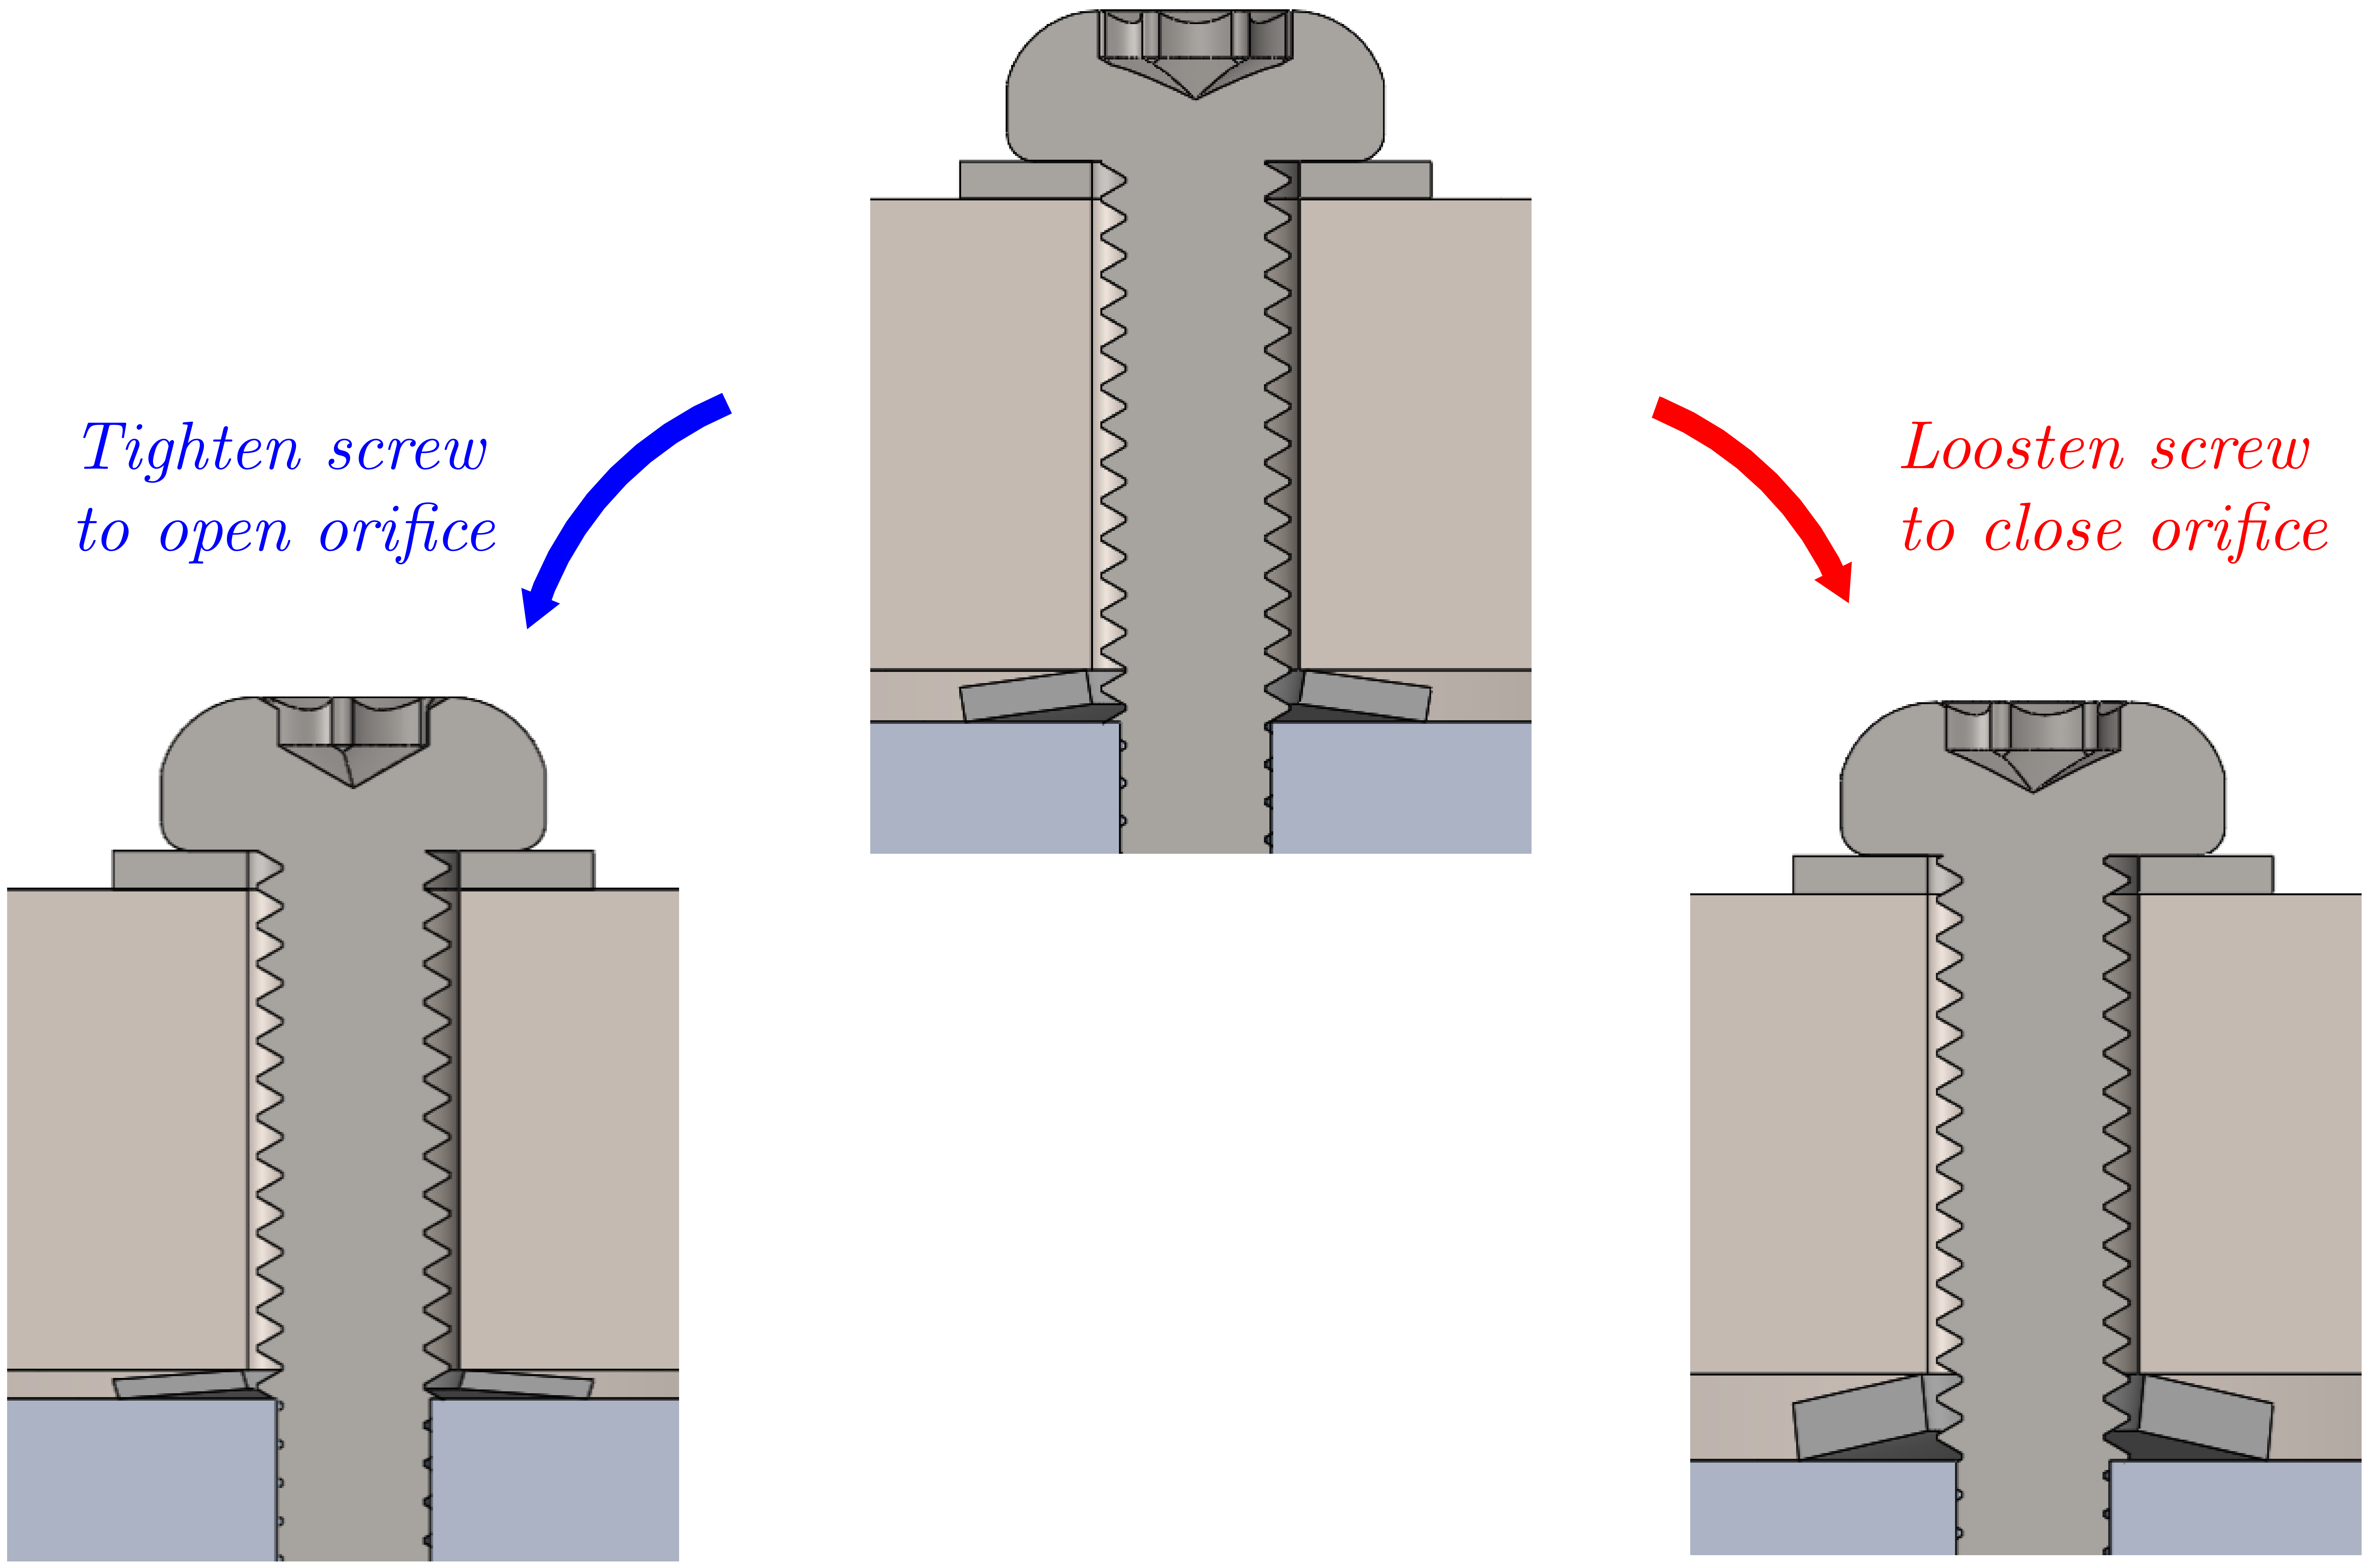
\includegraphics[width=.75\textwidth]{cal.png}
		\caption{System Calibration with a belleville washer, repeated}
		\label{fig:ug_calib}
	\end{figure}


	Depressurize the system before calibrating. Measure the orifice diameter at $T_\mathrm{ref} = \SI{25}{\degreeCelsius}$ using the sponsor-provided optical procedure and calculate the required height correction. Adjust the T6 adjustment screw in minute increments to achieve the target effective diameter. Refer to Figure~\ref{fig:ug_calib} for guidance.
	\begin{warningbox}
	\textbf{\textcolor{warnred}{CAUTION:}} Do not over-tighten the calibration screw on top of the actuator. It pre-loads a belleville washer inside the assembly.
	\end{warningbox}

	%-------------------------------------------------------------------
	\section{Operation}
	%-------------------------------------------------------------------

	\begin{figure}[htbp]
		\centering
	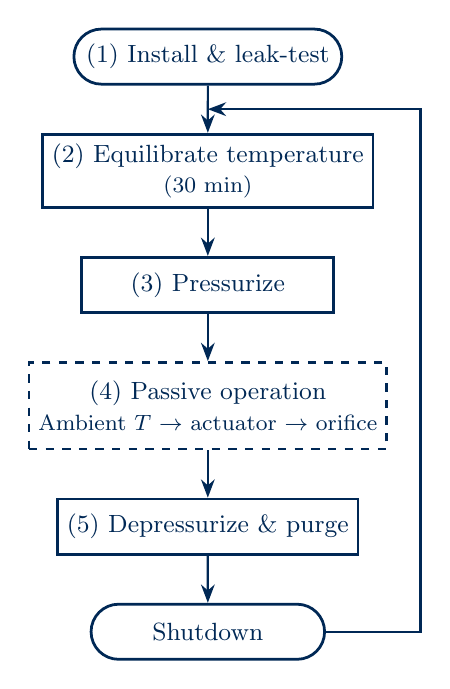
\begin{tikzpicture}[
			>=Stealth,
			node distance=0.6cm,
			font=\small,
			color=ucdblue,
			% Flowchart node styles
			startstop/.style={
				draw, rounded rectangle,
				minimum width=3.2cm, minimum height=0.7cm,
				align=center, color=ucdblue,
				line width=1pt
			},
			process/.style={
				draw, rectangle,
				minimum width=3.2cm, minimum height=0.7cm,
				align=center, color=ucdblue,
				line width=1pt
			},
			passive/.style={
				draw, rectangle,
				minimum width=3.2cm, minimum height=1.1cm,
				align=center, color=ucdblue,
				line width=1pt, dashed
			},
			arrow/.style={->, >=Stealth, color=ucdblue, line width=0.8pt}
		]

		% Nodes (top to bottom)
		\node[startstop] (install)
			{(1) Install \& leak-test};

		\node[process, below=of install] (equil)
			{(2) Equilibrate temperature\\{\footnotesize(30 min)}};

		\node[process, below=of equil] (press)
			{(3) Pressurize};

		\node[passive, below=of press] (passive)
			{(4) Passive operation\\
			{\footnotesize Ambient $T$ $\rightarrow$ actuator $\rightarrow$ orifice}};

		\node[process, below=of passive] (depress)
			{(5) Depressurize \& purge};

		\node[startstop, below=of depress] (end)
			{Shutdown};

		% Arrows
		\draw[arrow] (install)  -- (equil);
		\draw[arrow] (equil)    -- (press);
		\draw[arrow] (press)    -- (passive);
		\draw[arrow] (passive)  -- (depress);
		\draw[arrow] (depress)  -- (end);

		% Loop: Shutdown → midpoint of install→equil arrow
		\coordinate (loop-target) at ($(install.south)!0.5!(equil.north)$);
		\draw[arrow]
			(end.east)
			-- ++(1.2, 0)
			|- (loop-target);

		\end{tikzpicture}
		\caption{PTCD concept of operations.}
		\label{fig:ug_conops}
	\end{figure}

	\begin{enumerate}[leftmargin=1.8em, itemsep=6pt]

		\item \textbf{Install and leak-test} per Sections~4 and~5.

		\item \textbf{Equilibrate.} With the system at low pressure and the downstream valve closed, wait at least \textbf{60~minutes} or until the ambient temperature has been stable.

		\item \textbf{Check conditions.} Record the ambient temperature and confirm it is within \SI{-60}{\degreeCelsius} to \SI{+80}{\degreeCelsius}. Confirm the upstream pressure is within the rated range.

		\item \textbf{Pressurize.} Slowly open the upstream supply to the desired operating pressure. Do not exceed \SI{68.95}{\mega\pascal}.

		\item \textbf{Operate.} No further action is required. The PTCD adjusts the orifice automatically as temperature changes.

		\item \textbf{Shutdown.} Close the upstream supply valve and open the downstream vent to relieve pressure. Verify depressurisation with a gauge. If hydrogen was used, purge the lines before disconnecting any fittings. Repeat as in Figure~\ref{fig:ug_conops}.

	\end{enumerate}


	%-------------------------------------------------------------------
	\section{Quick-Reference Parameters}
	%-------------------------------------------------------------------

	\begin{center}
	\begin{tabular}{lll}
	\toprule
	\textbf{Parameter} & \textbf{Value} & \textbf{Notes} \\
	\midrule
	Reference temperature $T_\mathrm{ref}$ & \SI{25}{\degreeCelsius} & Calibration point \\
	Operating temperature range & \SI{-60}{\degreeCelsius} to \SI{+80}{\degreeCelsius} & Ambient at actuator \\
	Orifice diameter at \SI{-60}{\degreeCelsius} & $383.5 \pm 19.2\,\upmu$m & Maximum open \\
	Orifice diameter at \SI{+25}{\degreeCelsius} & $254.0 \pm 12.7\,\upmu$m & Reference \\
	Orifice diameter at \SI{+80}{\degreeCelsius} & $170.2 \pm 16.9\,\upmu$m & Minimum open \\
	Max.\ operating pressure & \SI{68.95}{\mega\pascal} (\num{10000}~psi) & \\
	Min.\ operating pressure & \SI{689.5}{\kilo\pascal} (\num{100}~psi) & \\
	Compatible gases & Noble gases, H$_2$ & All wetted parts H$_2$-rated \\
	\bottomrule
	\end{tabular}
	\end{center}

	\renewcommand{\thesection}{\thechapter.\arabic{section}}
	\addtocontents{toc}{\protect\setcounter{tocdepth}{2}}

\chapter{Engineering Drawing Package}
\label{app:drawings}

	Tolerances listed in the following drawings are taken from HAAS VF-2 series specifications \cite{ref_haas}.
	Refer to Appendices~\ref{app:mfg} and \ref{app:op} for manufacturing and operation guides.

	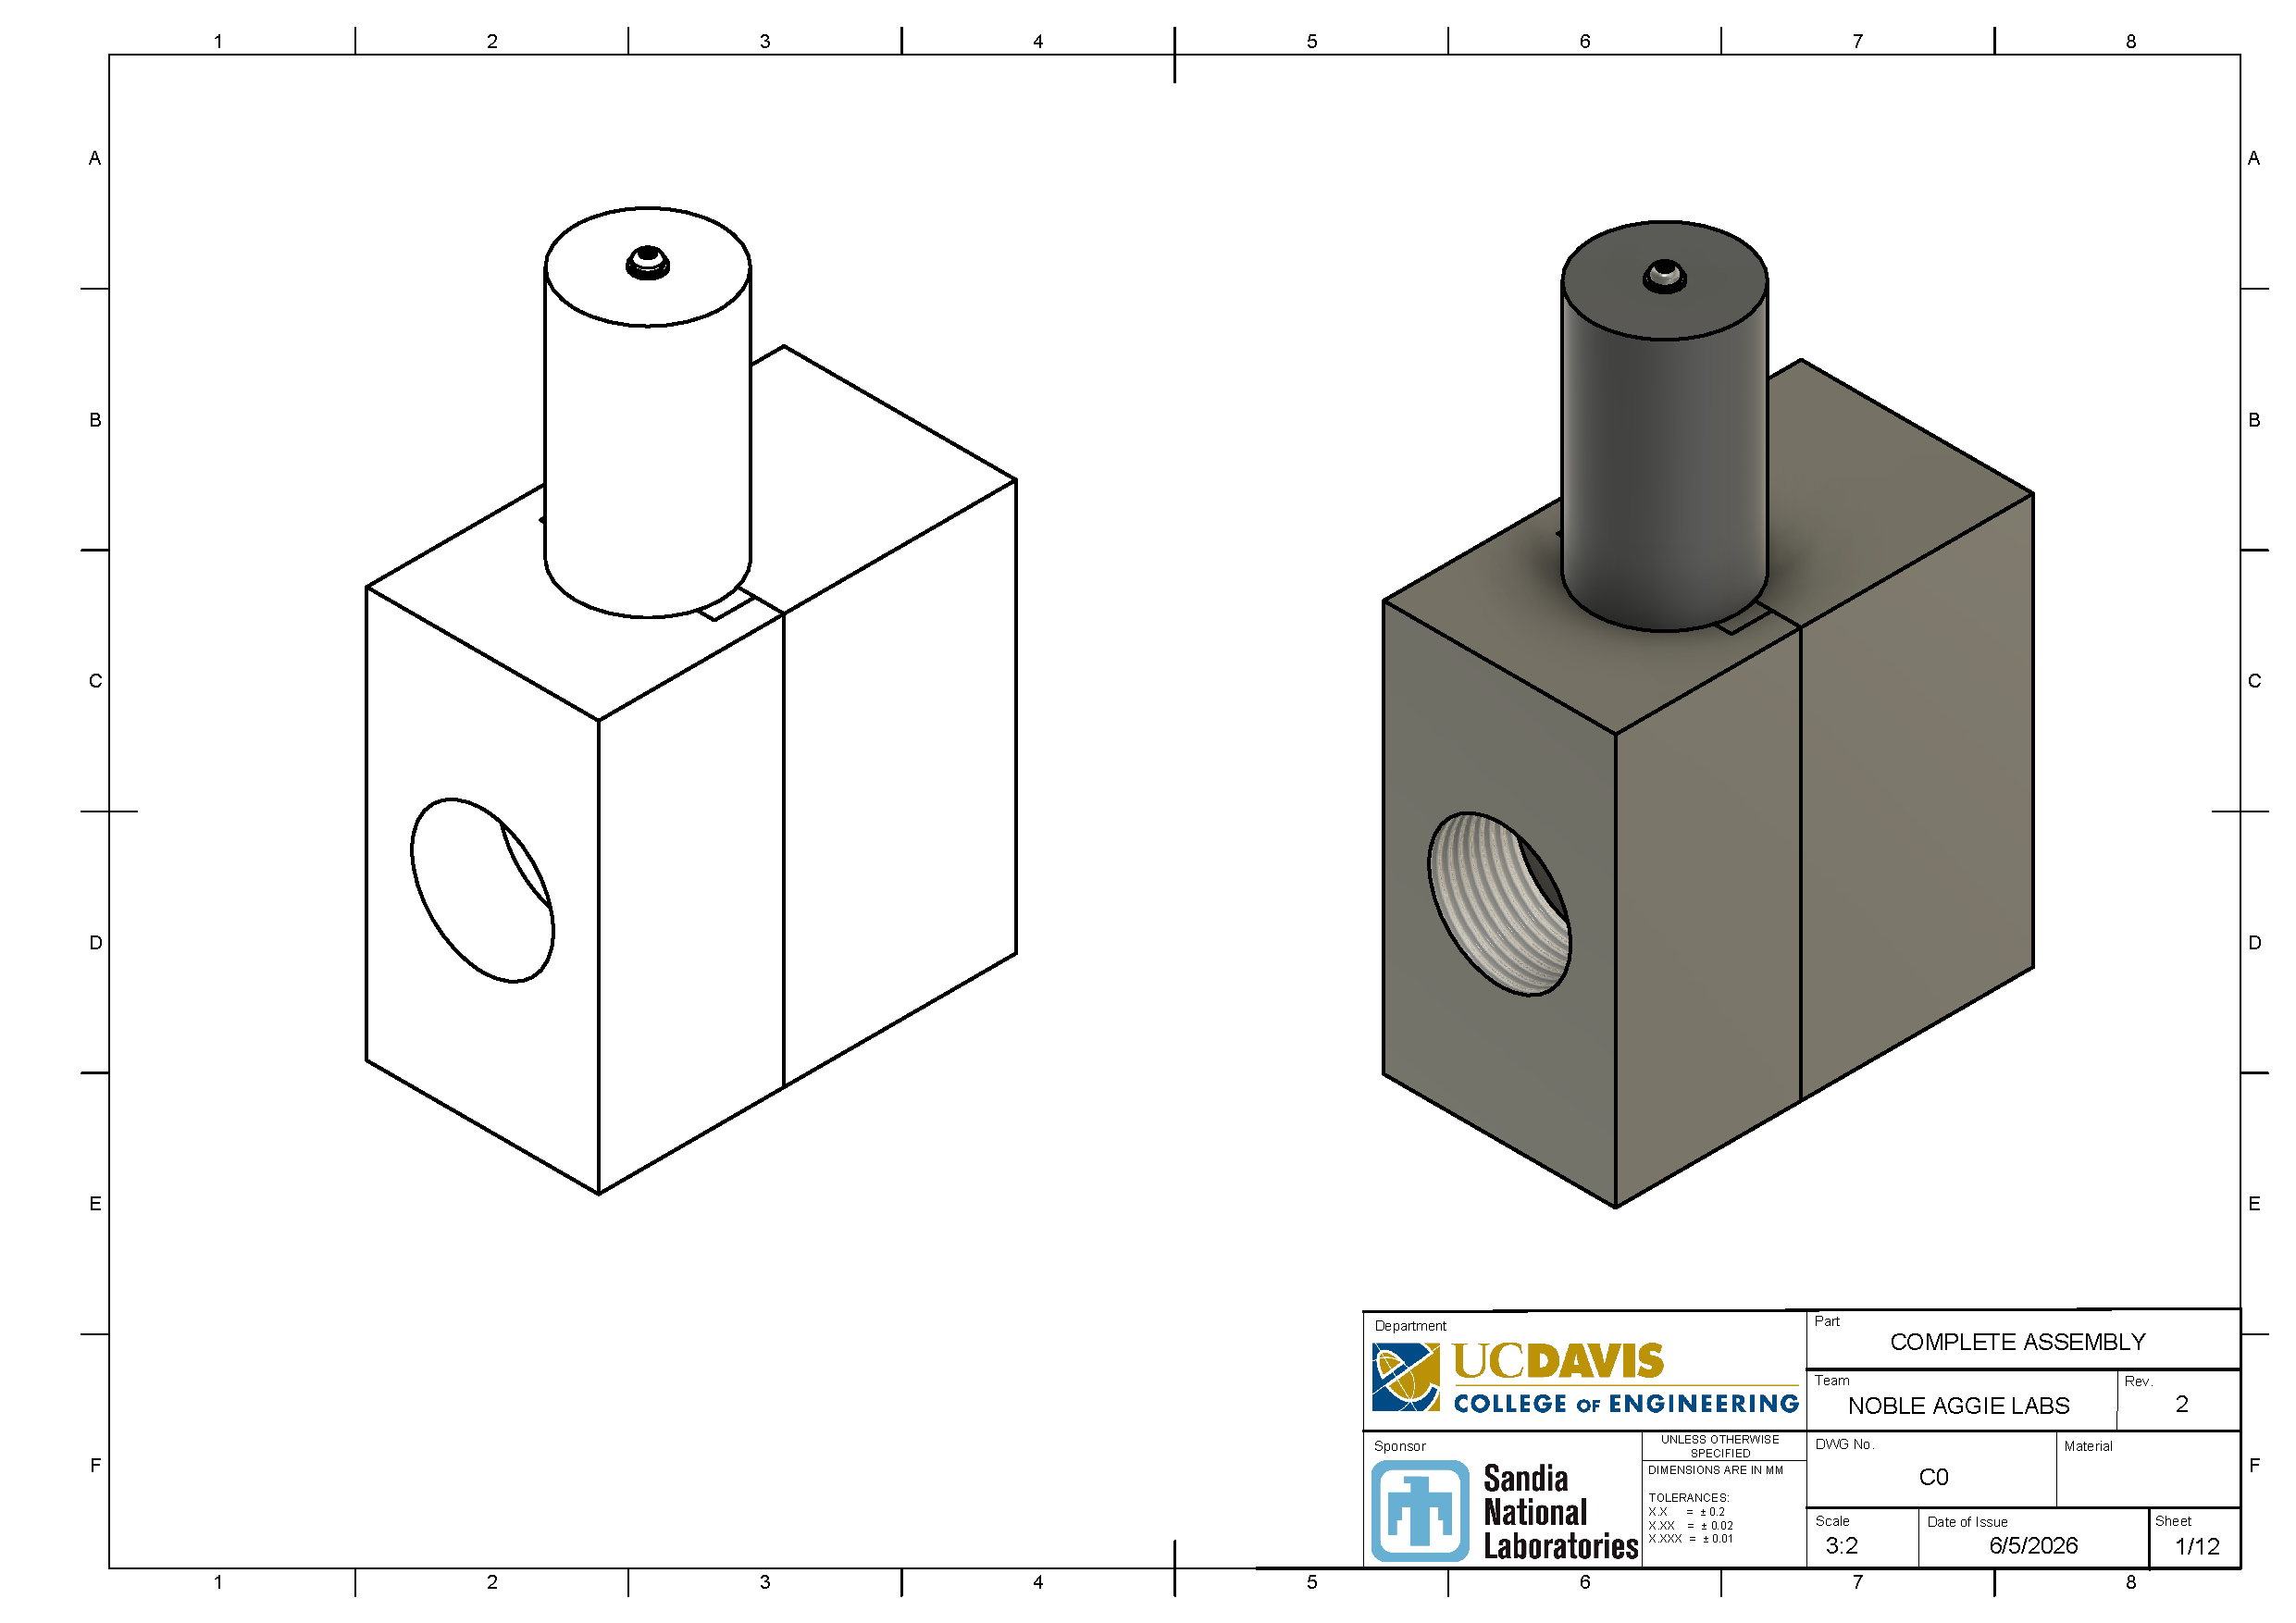
\includepdf[pages=1-12, fitpaper=true, landscape=true]{06052026_FinalDrawingPackage.pdf}

\chapter{Data Sheets}
\label{app:datasheets}

	The following information is provided below:

	\begin{enumerate}
		\item Part drawings and specifications for the screw, standard washer, and belleville washer
		\item Bellows part specifications (excerpt from Mini-Flex's 2026 metal bellows catalog)
		\item Material data sheets
	\end{enumerate}

	\newpage
	\section{McMaster Part Drawings and Specifications}
	\label{app:datasheets:McMaster}

		Source: McMaster Carr\cite{ref_McMaster_screw, ref_McMaster_std, ref_McMaster_belle}.
	
		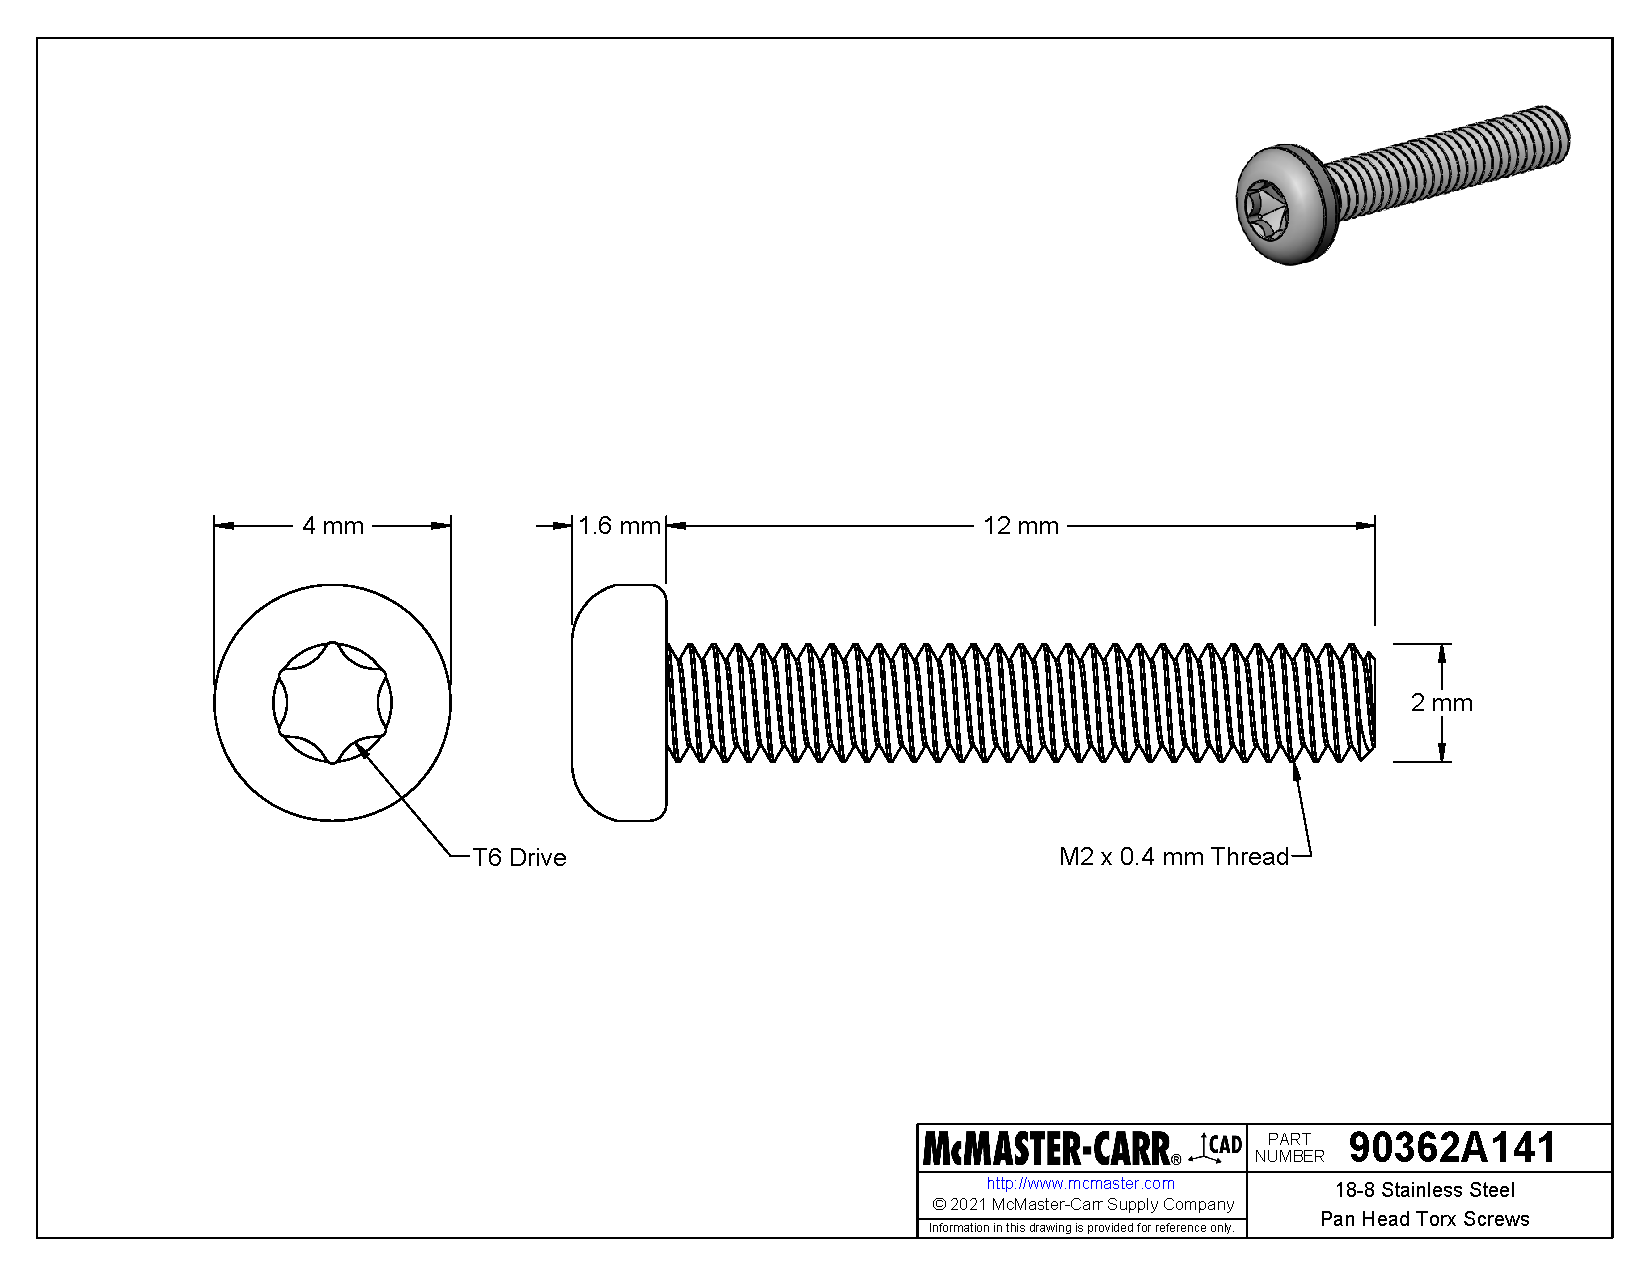
\includepdf[fitpaper=true, landscape=true]{pdf/90362A141_drawing.pdf}
		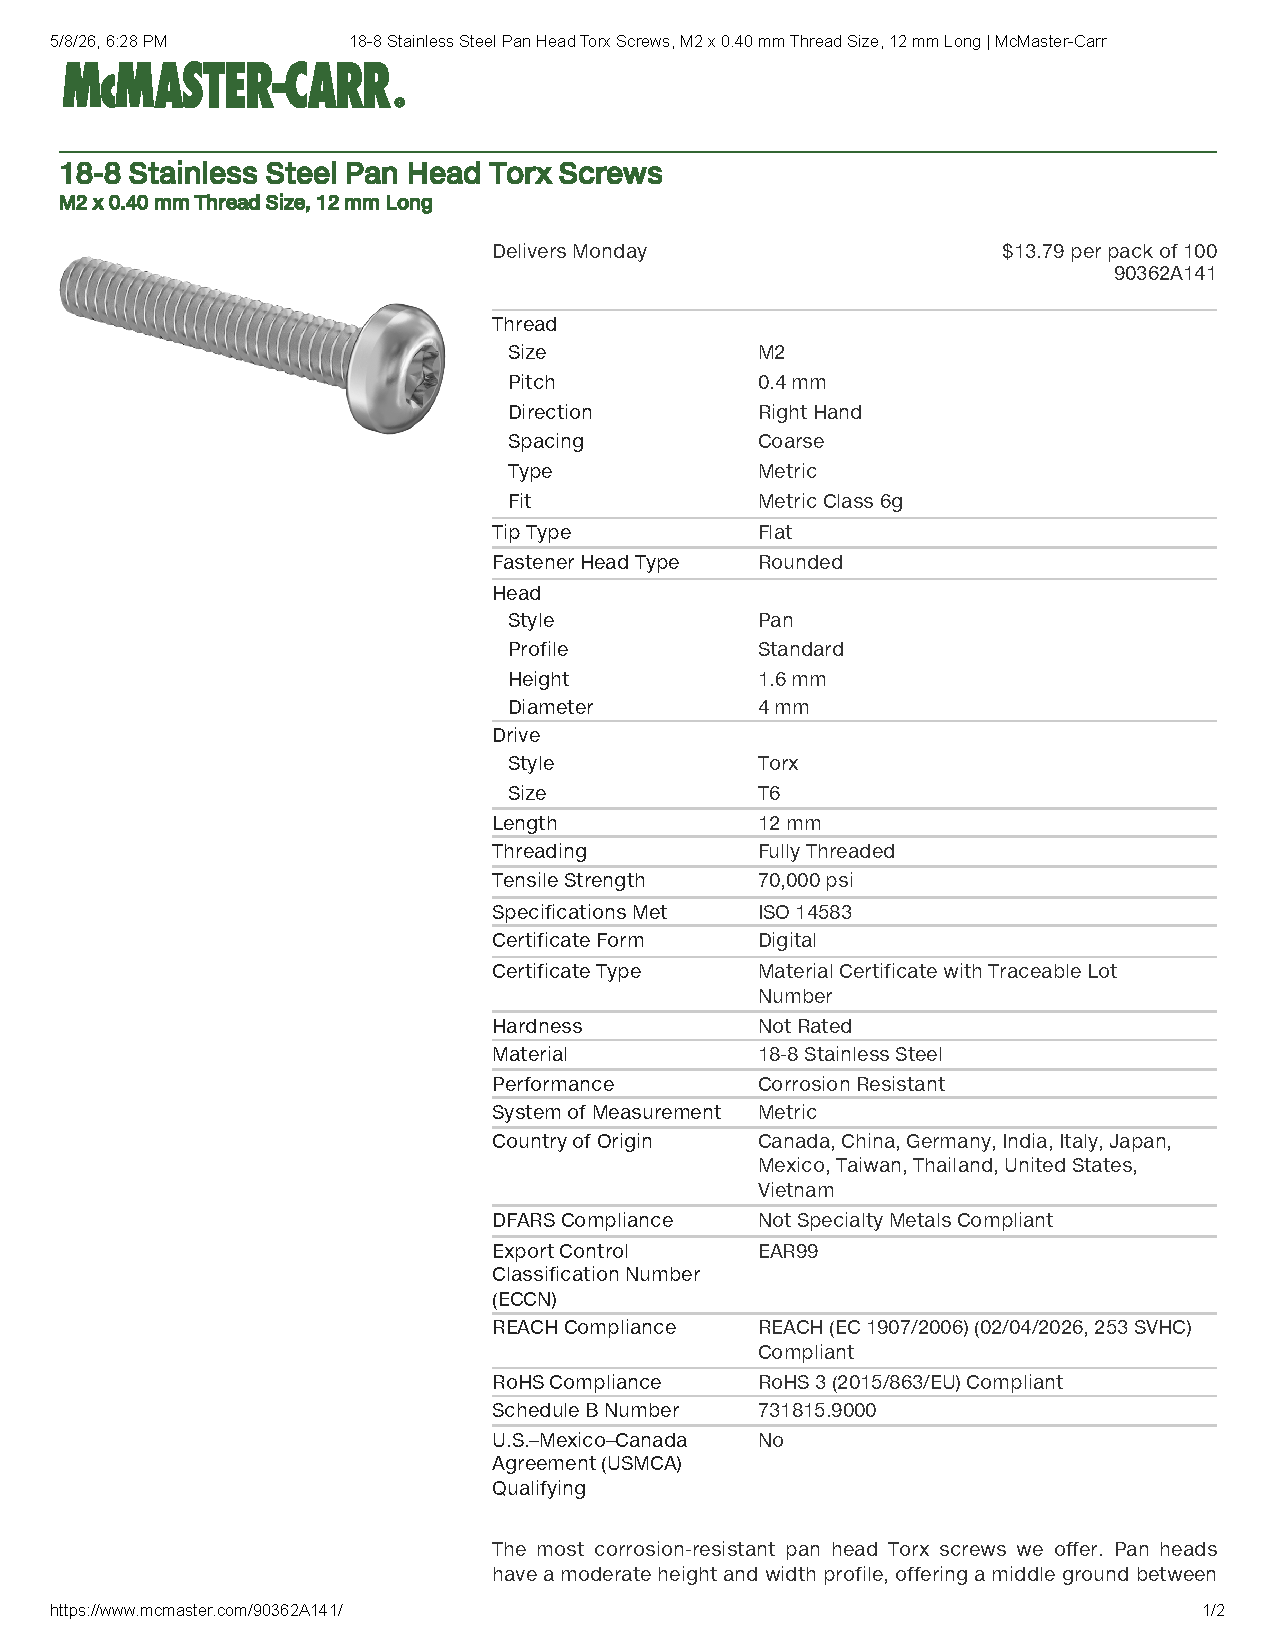
\includepdf[pages=1, fitpaper=true, landscape=true]{pdf/90362A141_specs.pdf}
		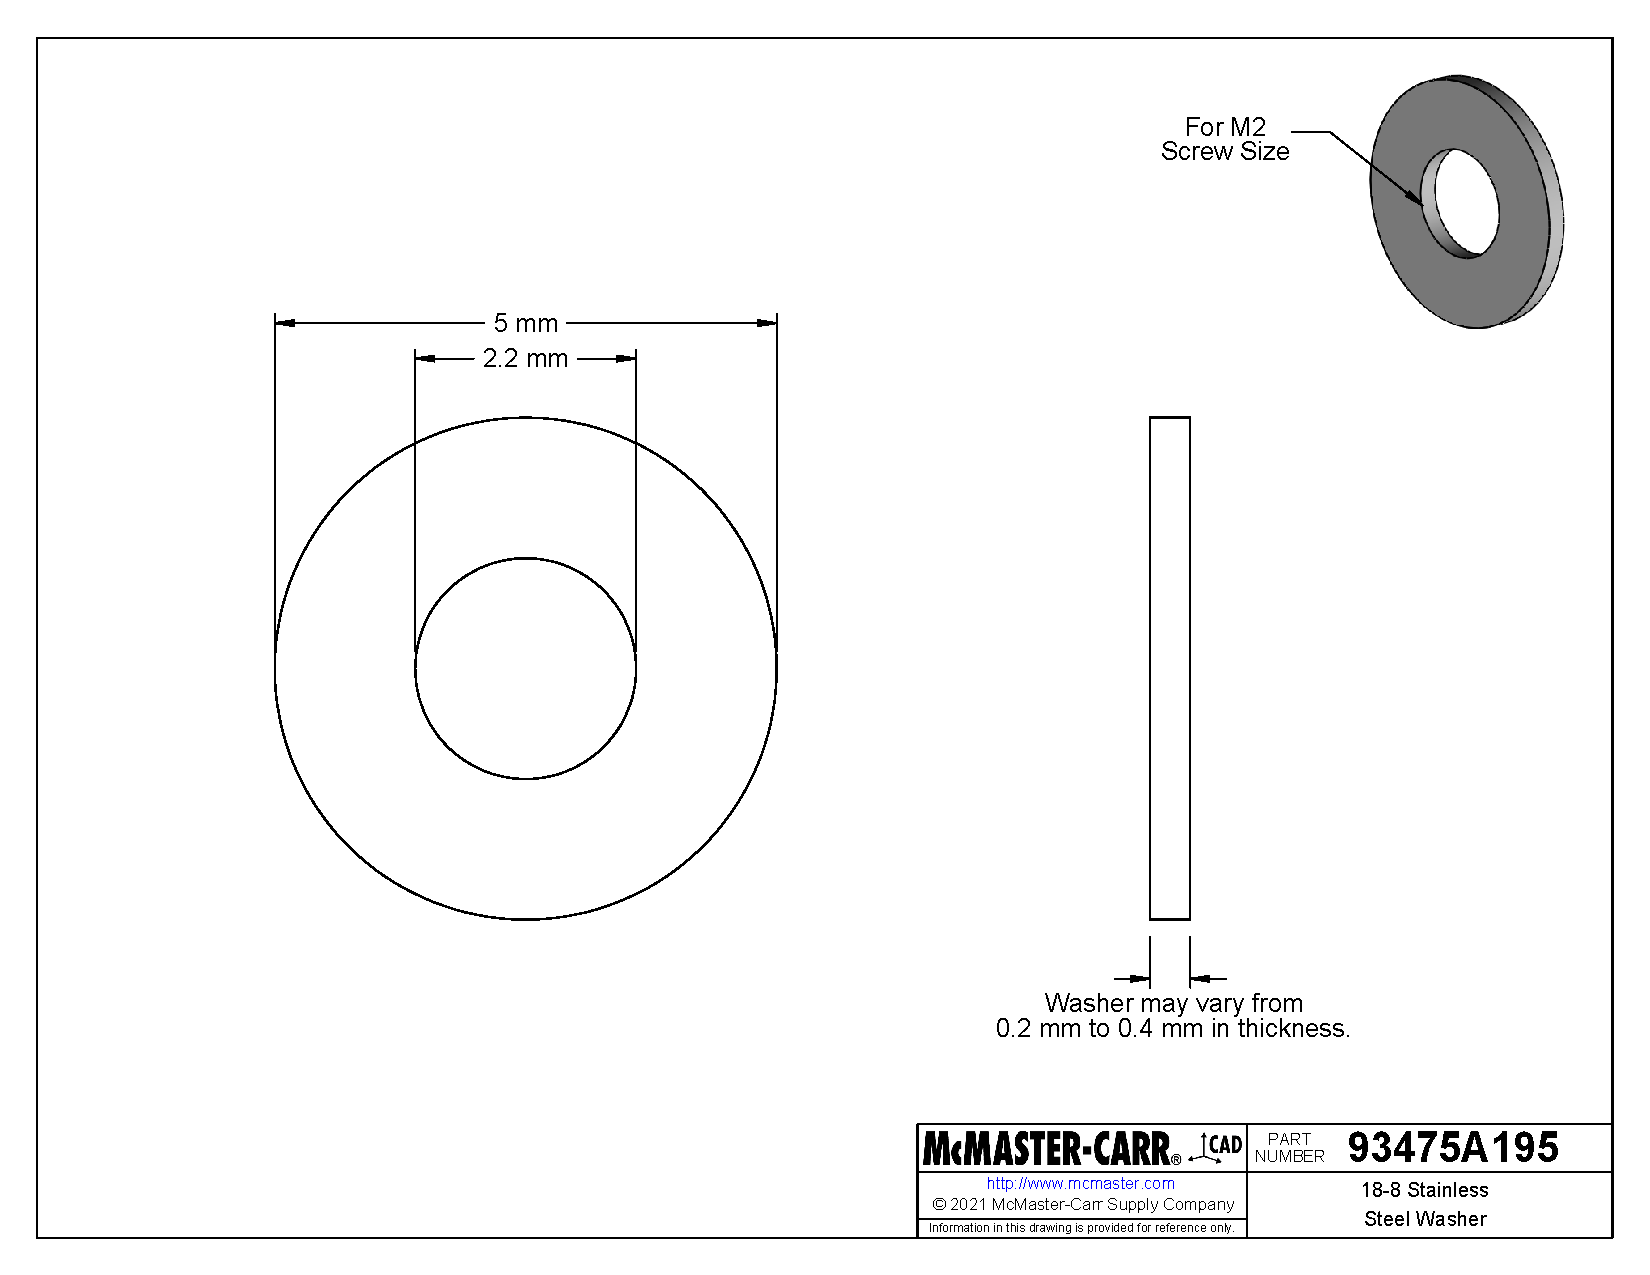
\includepdf[fitpaper=true, landscape=true]{pdf/93475A195_drawing.pdf}
		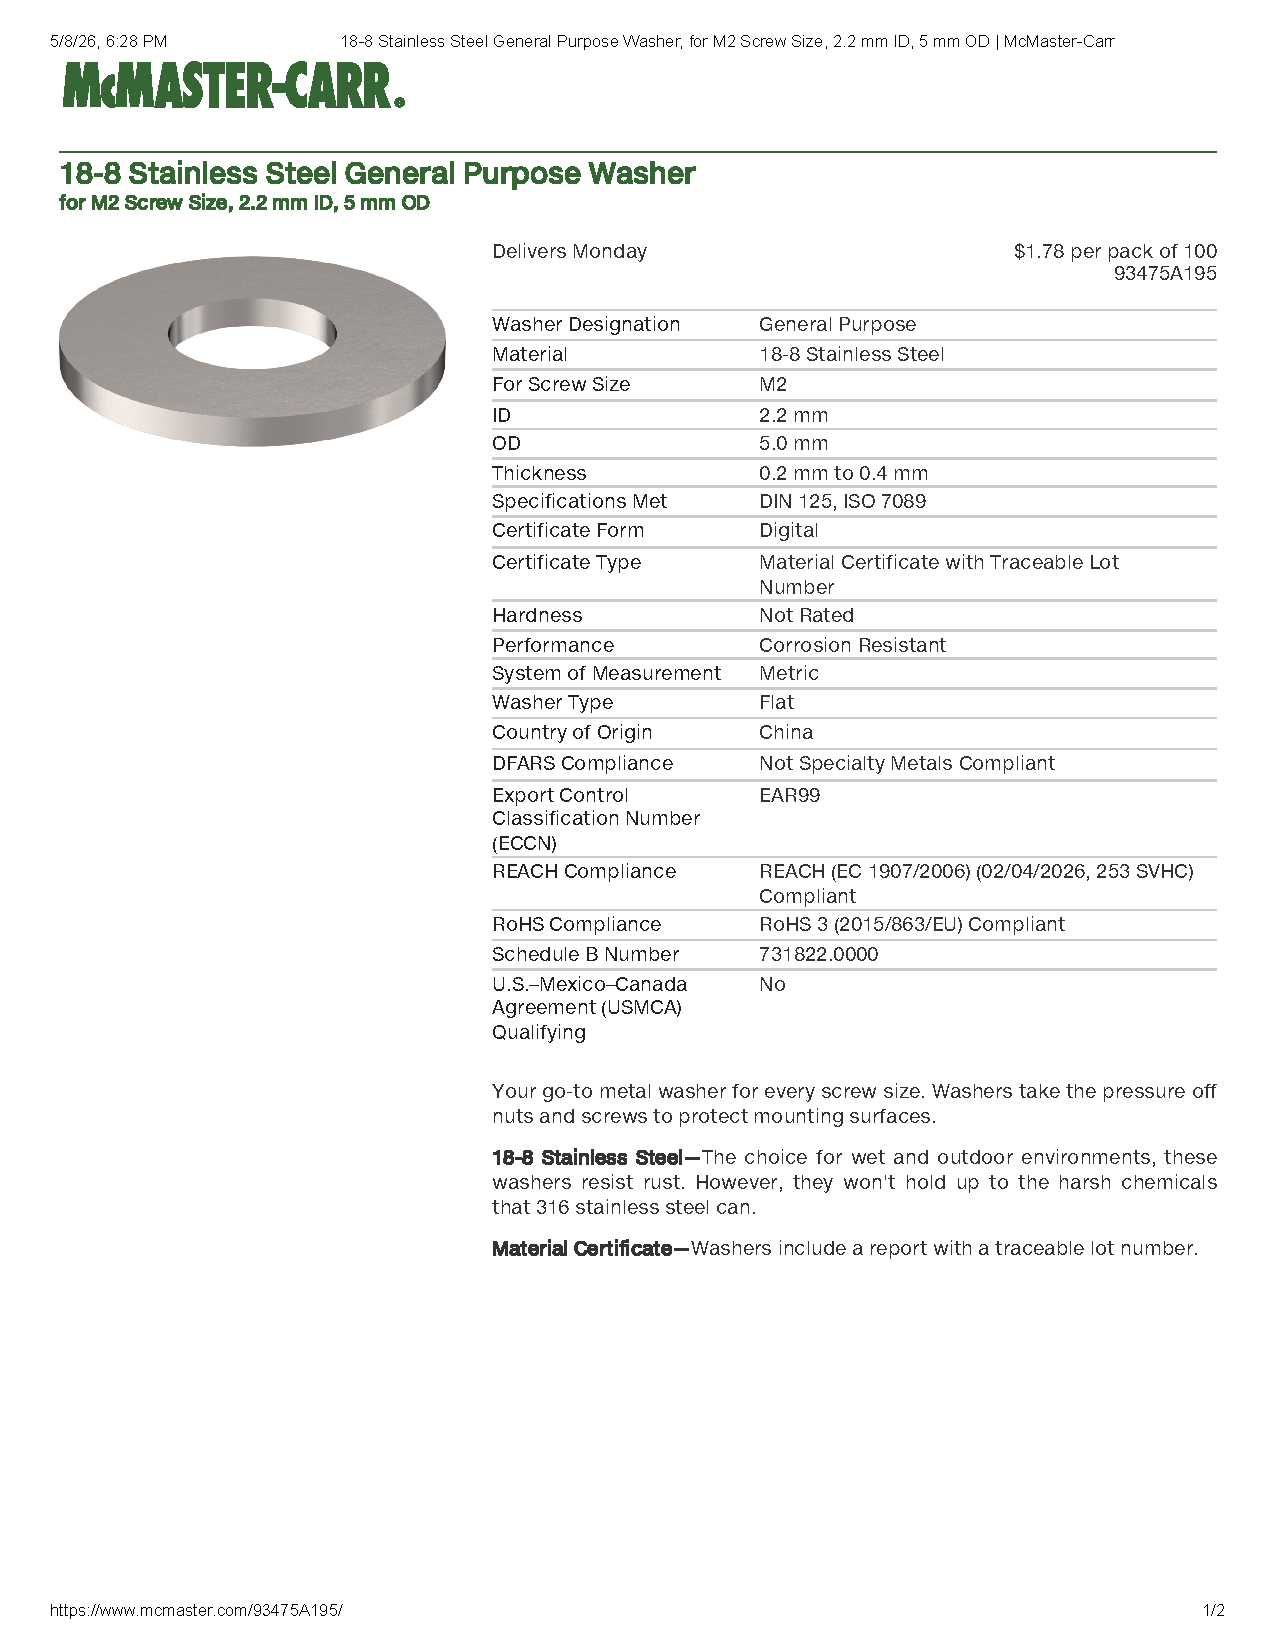
\includepdf[pages=1, fitpaper=true, landscape=true]{pdf/93475A195_specs.pdf}
		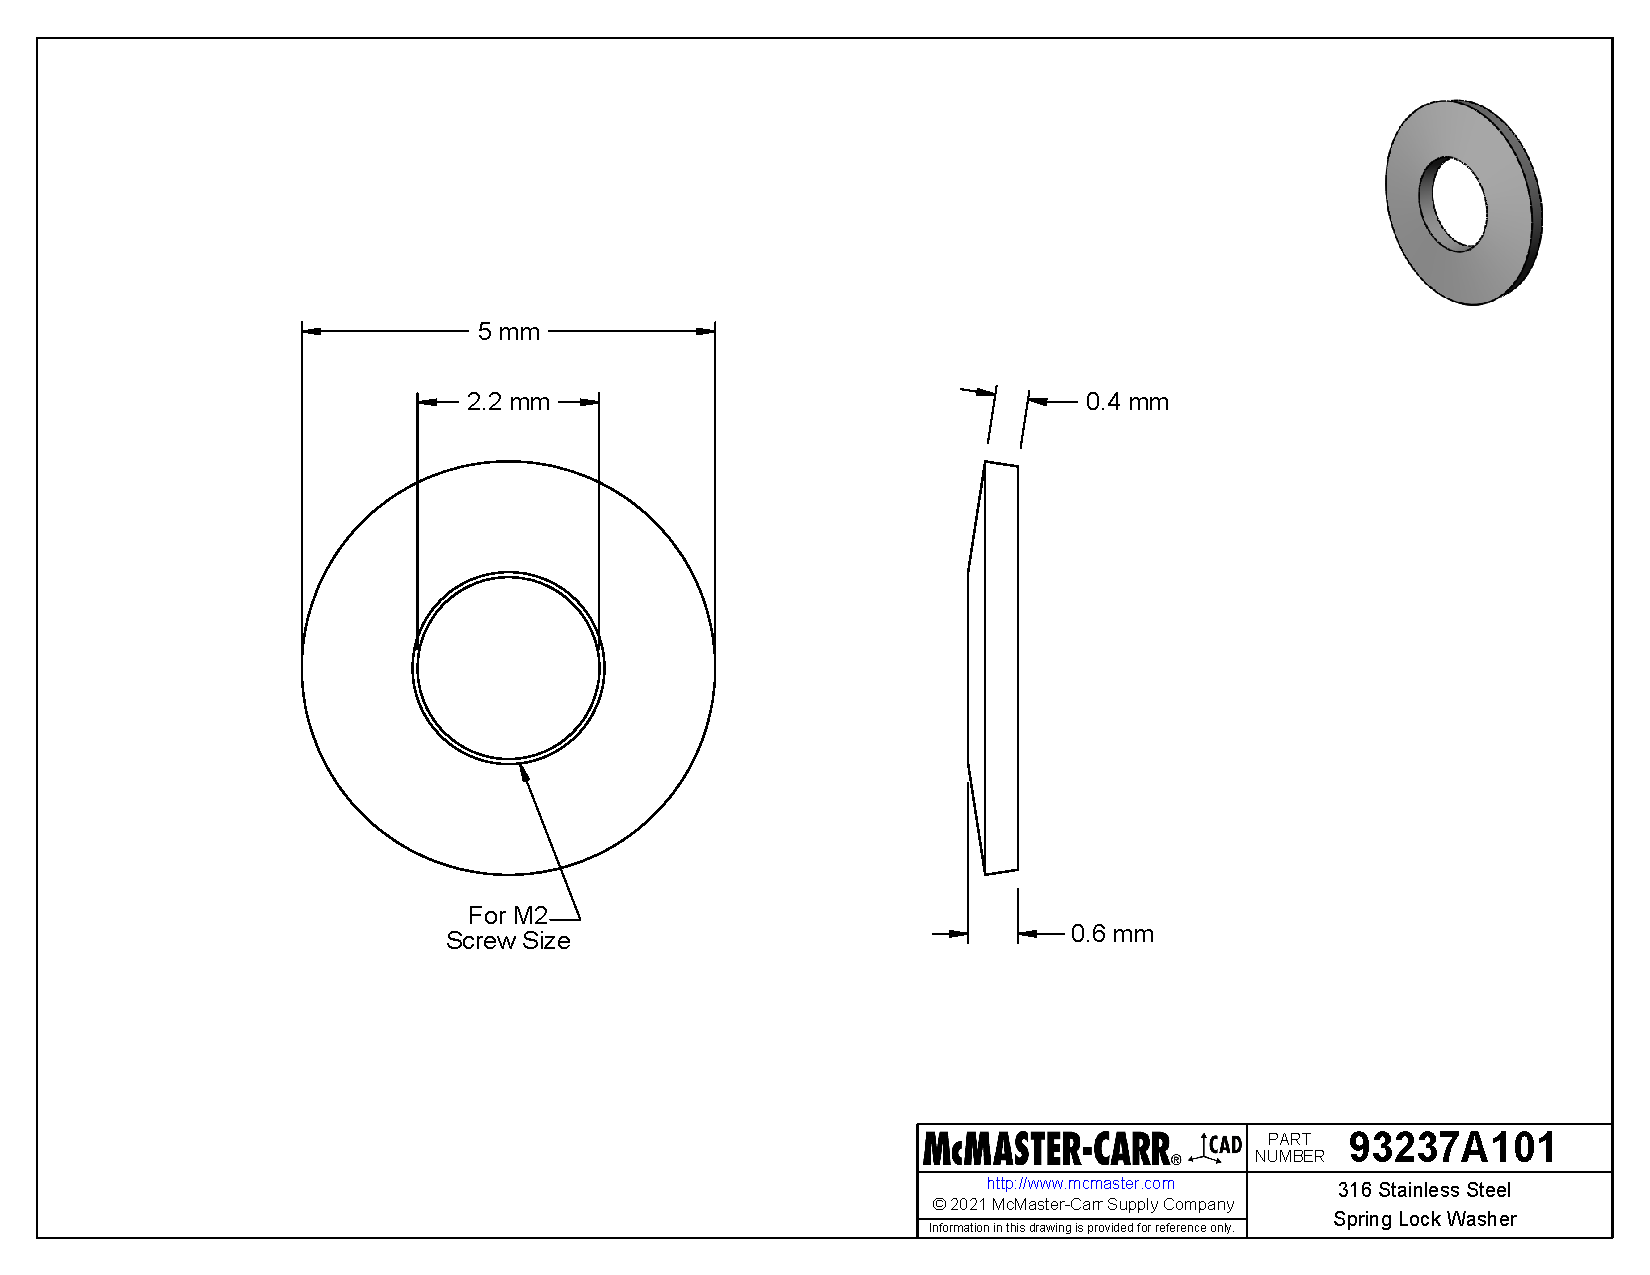
\includepdf[fitpaper=true, landscape=true]{pdf/93237A101_drawing.pdf}
		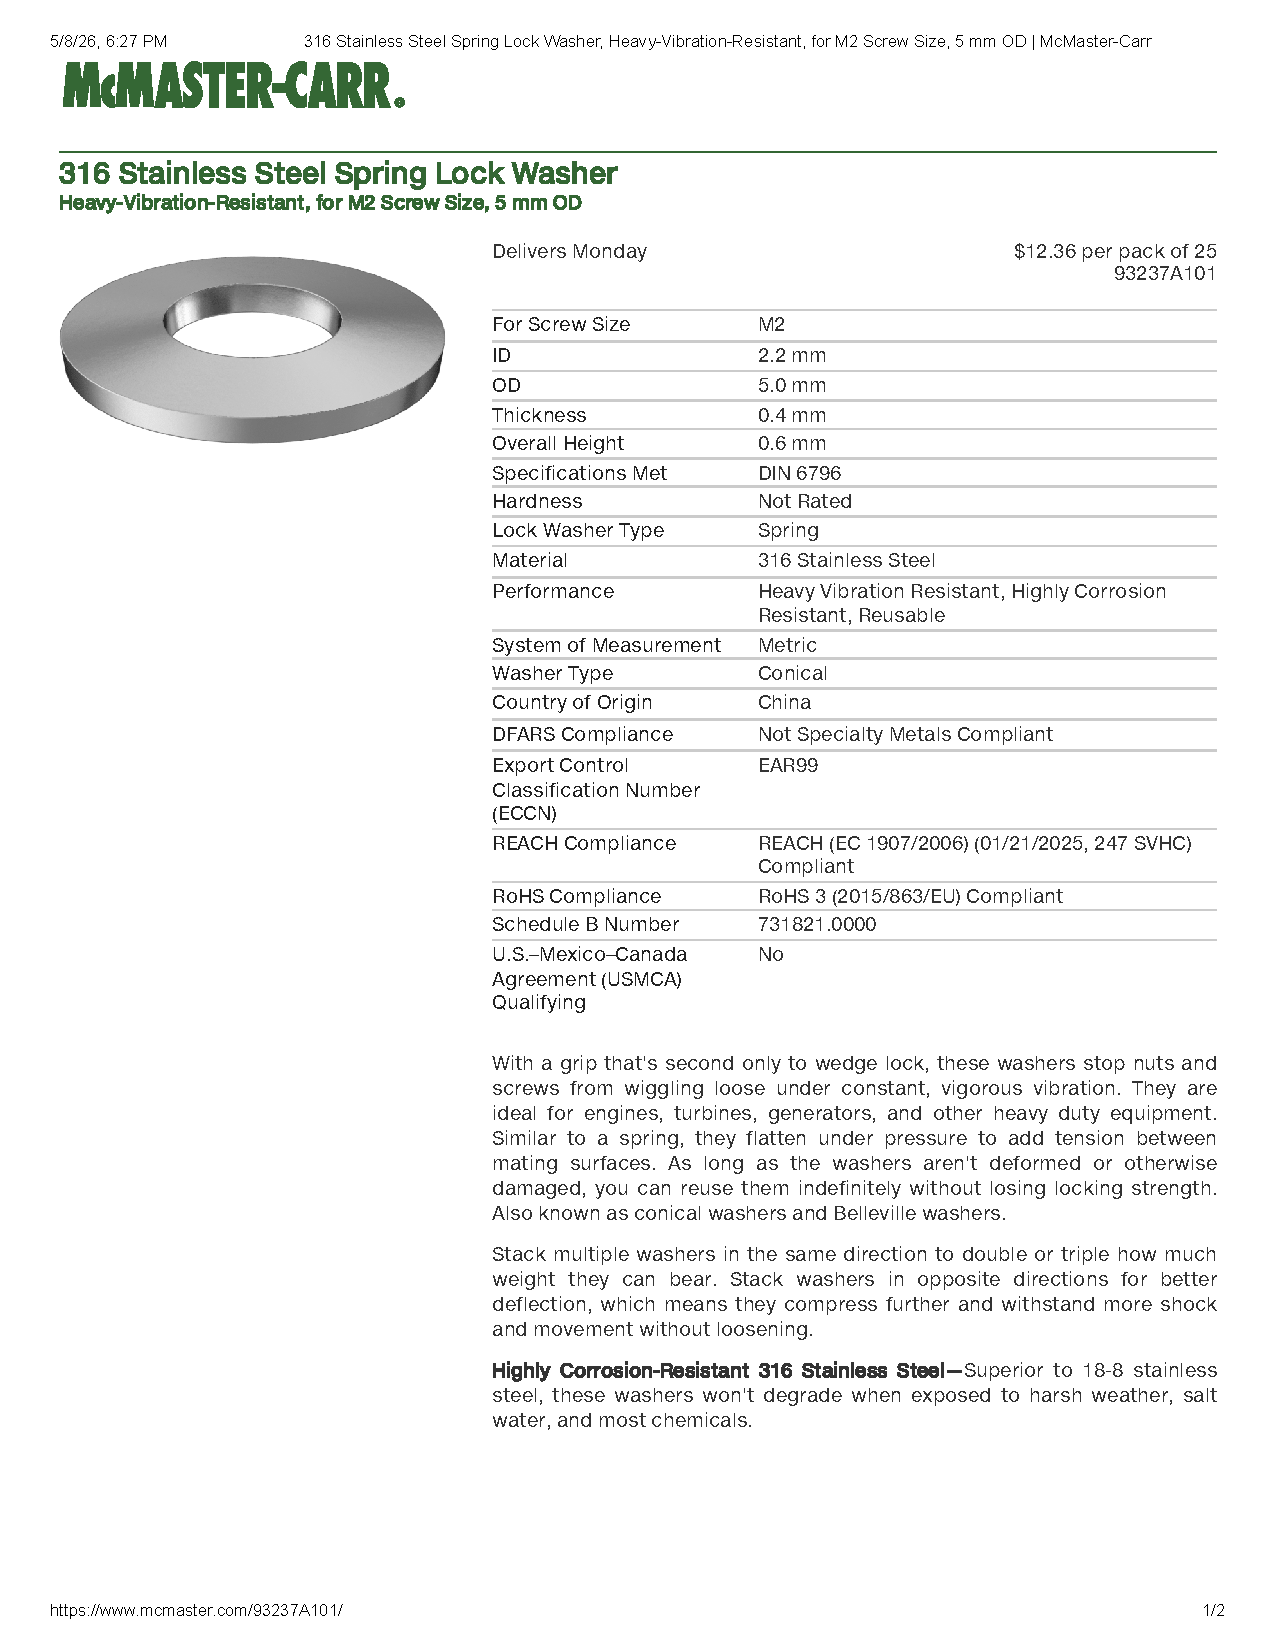
\includepdf[pages=1, fitpaper=true, landscape=true]{pdf/93237A101_specs.pdf}

	\section{Bellows Specifications}
	\label{app:datasheets:Bellows}

		Source: Mini-Flex Corporation\cite{ref_miniflex_catalog}. See also the Design Guide\cite{ref_miniflex_design}.
		Note that although the squirm pressure rating, \specBellowsSquirm, is less than the pressure capacity stipulated by Specification \specref{V.3.2} (\specPressure), the Design Guide states that ``squirm will not occur if the bellows is guided internally or externally by a rod stem or in a close fitting bore''\cite[p.~5]{ref_miniflex_design}.
		The valve stem provides such support, dimensioned to provide a sliding-fit interface (see Section~\ref{subsec:design:just:fits}).

		
\includepdf[pages=1-2, fitpaper=true, landscape=true]{pdf/I718-159-72-430.pdf}

	\section{Material Properties}
	\label{app:datasheets:mat}

    Below are the material properties used throughout this report:
    Aluminum 6061\cite{ref_NASA_specs_Al},
    ALLVAR\cite{ref_AllvarAlloys},
    Invar 36\cite{ref_Carpenter_Inv},
    Inconel 718\cite{ref_SpecialMetals_Inc}, and
    316 Stainless Steel\cite{ref_Ledbetter_Stainless}.
		Properties listed are the Coefficient of Thermal Expansion $\alpha$, Thermal Conductivity $k$, Young's Modulus $E$, and Poisson's Ratio $\nu$.
		
		\begin{table}[H]
			\centering
			\caption{Material Properties}
			\renewcommand{\arraystretch}{1.3}
			\begin{tabularx}{\textwidth}{
				>{\raggedright\arraybackslash}p{0.22\textwidth}
				>{\centering\arraybackslash}X
				>{\centering\arraybackslash}X
				>{\centering\arraybackslash}X
				>{\centering\arraybackslash}X
				>{\centering\arraybackslash}X
			}
			\toprule
			\textbf{Material} &
			\textbf{$\alpha$} $\left(\si{\micro\meter\per\meter\per\degreeCelsius}\right)$ &
			\textbf{$k$} $\left(\si{\watt\per\meter\per\degreeCelsius}\right)$ &
			\textbf{$E$} $\left(\si{\giga\pascal}\right)$ &
			\textbf{$\nu$} &
			\textbf{$c_p$} $\left(\si{\joule\per\kilogram\per\degreeCelsius}\right)$ \\
			\midrule

			Aluminum 6061
				& \num{22.85}
				& \num{167}
				& \num{68.95}
				& ---
				& \num{962} \\

			ALLVAR
				& \num{-30}
				& \num{8.88}
				& \num{55}
				& ---
				& --- \\

			Invar 36
				& \num{1.3}
				& \num{10.5}
				& \num{141}
				& ---
				& \num{515} \\

			Inconel 718
				& \num{13.2}
				& ---
				& \num{200}
				& ---
				& \num{435} \\

			316 Stainless Steel
				& ---
				& ---
				& \num{207.8}
				& \num{0.282}
				& --- \\

			\bottomrule
			\end{tabularx}
			\label{tab:mat_props}
		\end{table}

		\vspace{1em}
		\begin{table}[H]
			\centering
			\caption{Aluminum CTE as a Function of Temperature\cite{ref_NASA_specs_Al}}
			\label{tab:CTE_Al}
			\begin{tabular}{cc|cc}
				\toprule
				$T$ (\si{\degreeCelsius}) & $\alpha$ (\si{\micro\meter\per\meter\per\degreeCelsius}) &
				$T$ (\si{\degreeCelsius}) & $\alpha$ (\si{\micro\meter\per\meter\per\degreeCelsius}) \\
				\midrule
				$-60$ & 21.8  & $15$ & 22.75 \\
				$-55$ & 21.9  & $20$ & 22.8  \\
				$-50$ & 22.0  & $25$ & 22.85 \\
				$-45$ & 22.1  & $30$ & 22.9  \\
				$-40$ & 22.2  & $35$ & 23.0  \\
				$-35$ & 22.25 & $40$ & 23.1  \\
				$-30$ & 22.3  & $45$ & 23.15 \\
				$-25$ & 22.35 & $50$ & 23.2  \\
				$-20$ & 22.4  & $55$ & 23.25 \\
				$-15$ & 22.45 & $60$ & 23.3  \\
				$-10$ & 22.5  & $65$ & 23.35 \\
				$-5$  & 22.55 & $70$ & 23.4  \\
				$0$   & 22.6  & $75$ & 23.45 \\
				$5$   & 22.65 & $80$ & 23.5  \\
				$10$  & 22.7  &      &       \\
				\bottomrule
			\end{tabular}
		\end{table}

\chapter{Project Management}
\label{app:PM}

% \begin{figure}[H]
%     \centering
%     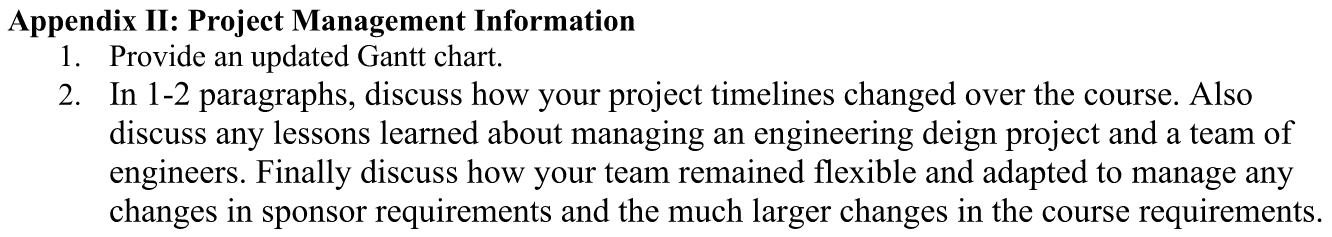
\includegraphics[width=\textwidth]{Del_app_reqs_2.png}
%     \caption{DELETE BEFORE SUBMITTING}
%     \label{fig:del_app_reqs_2}
% \end{figure}    

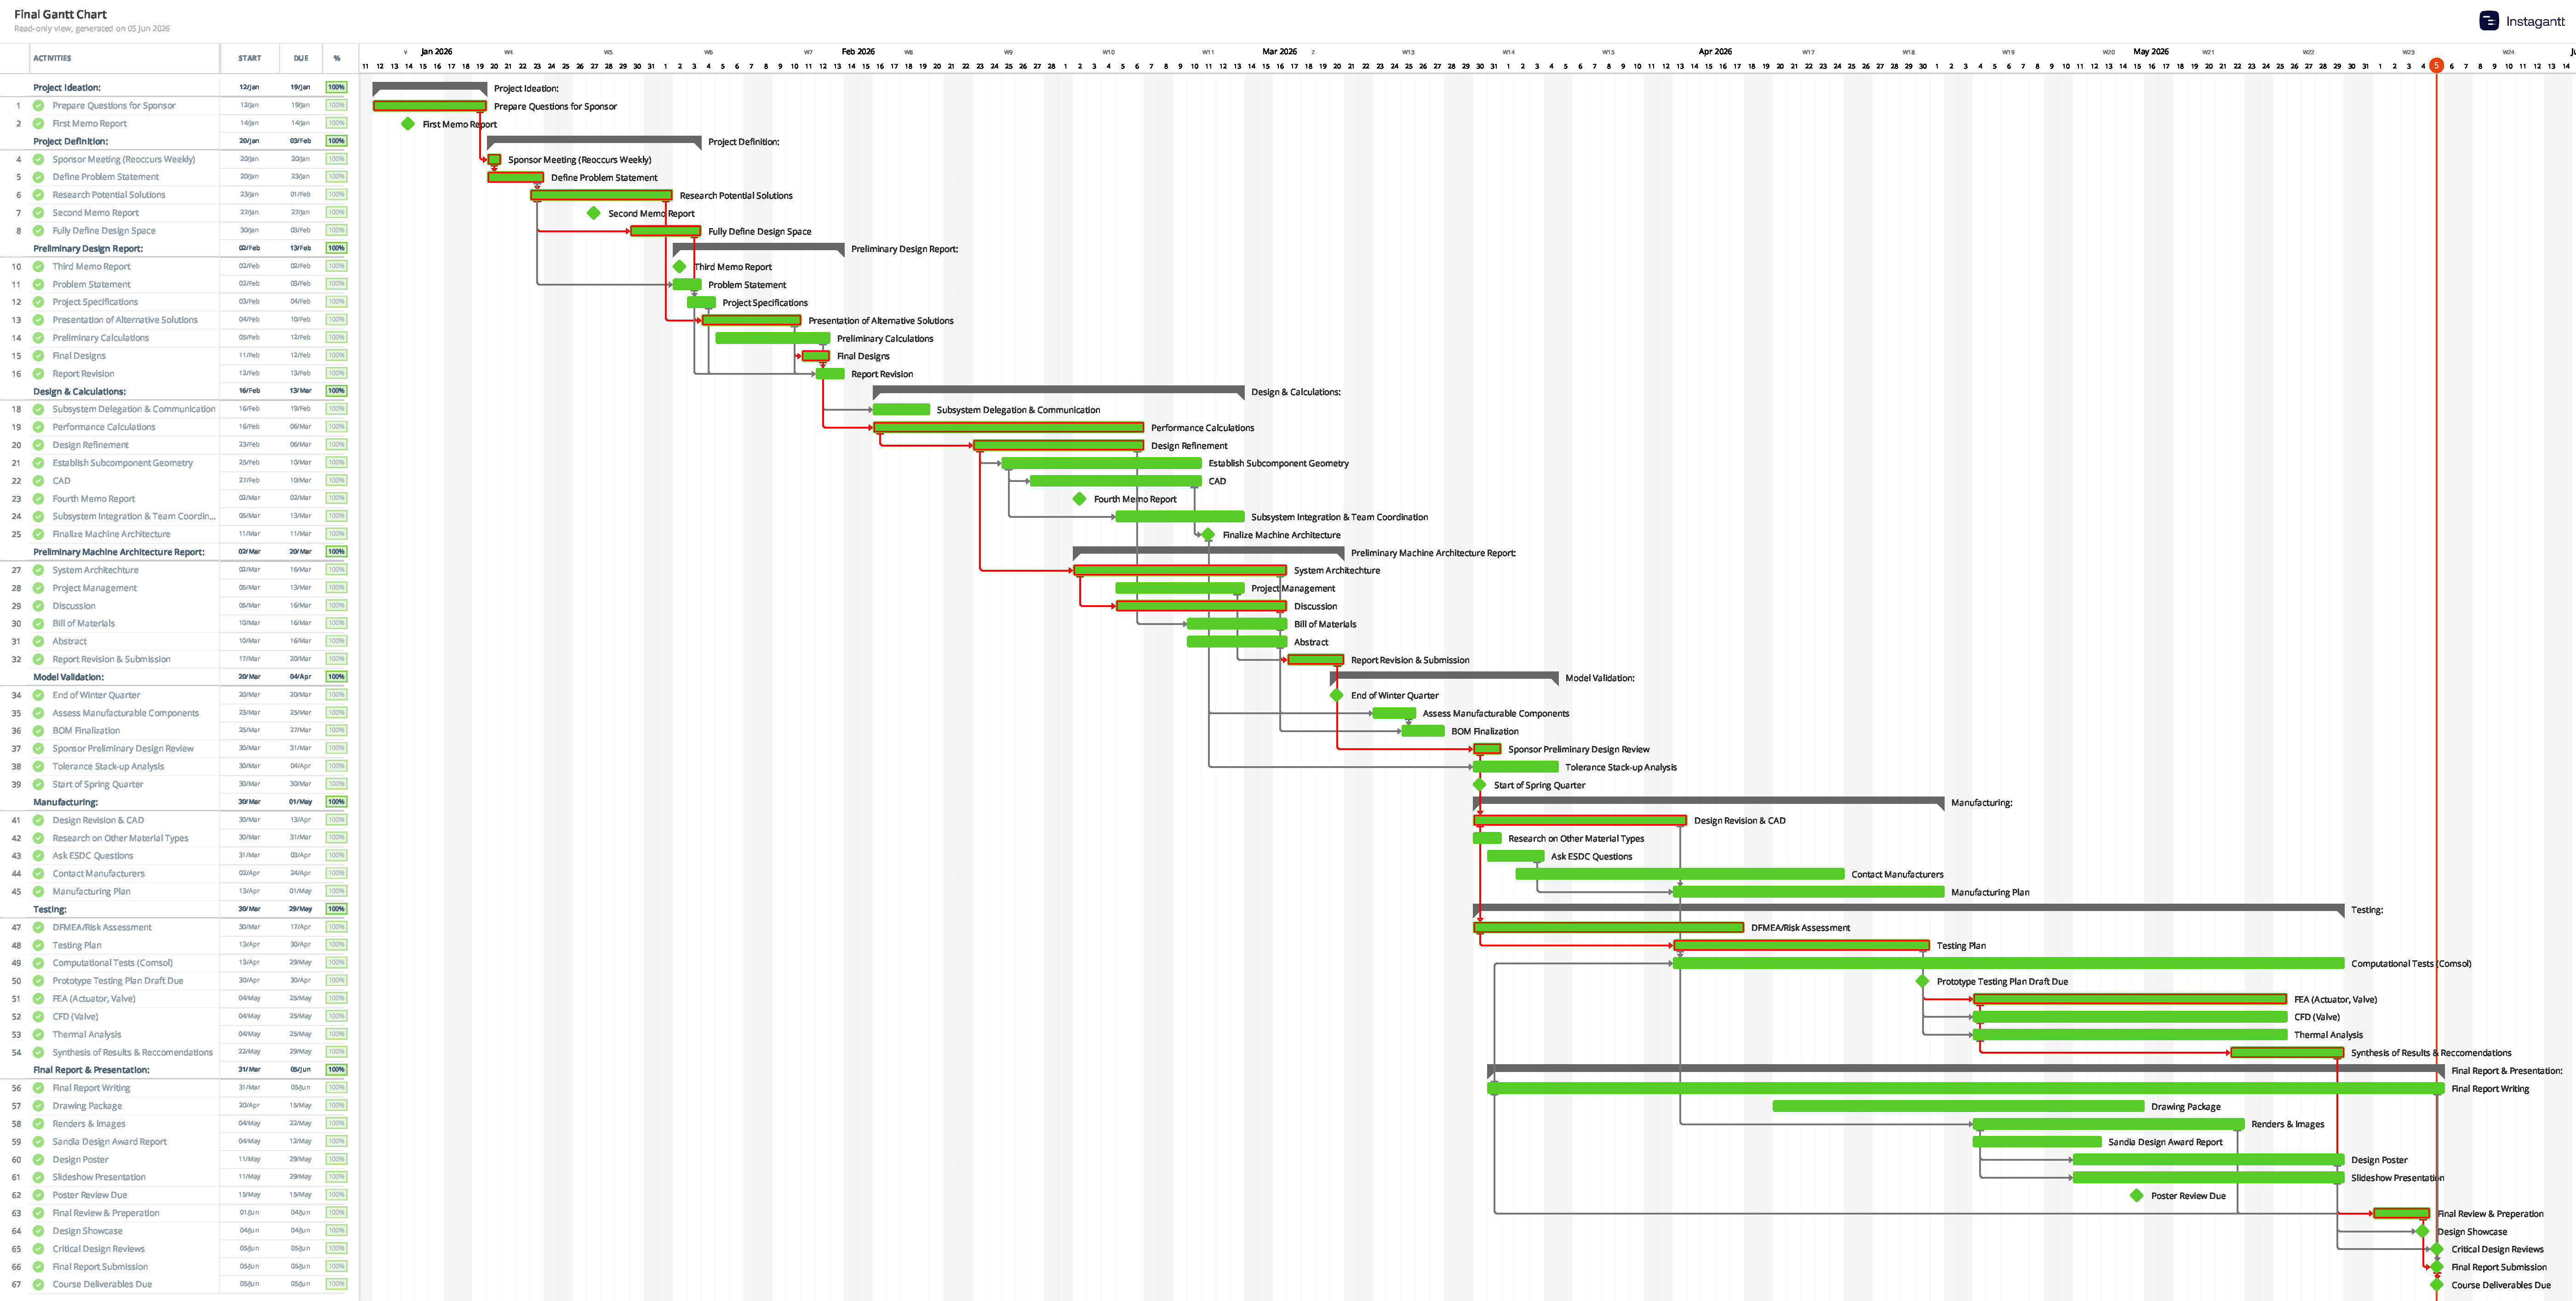
\includepdf[pages=1, fitpaper=true, landscape=true]{FinalGanttChart.pdf}

	Development of the \device\ was no small feat. Faced with a genuinely difficult engineering challenge, we accomplished in six months what most professionals would likely spend a year to develop.
	We developed four distinct iterated designs, each time addressing an unavoidable source of error, resolving a manufacturing conflict, or taking advantage of an unforeseen opportunity to make the device simpler and more robust.
	Through it all, our team learned more about engineering design and project management than we ever dreamed of. This design program equipped us for industry work far better than we could have asked or imagined.

	Our sponsor provided us with clear, unchanging system requirements and threw us very few curveballs. We are grateful for this. However, owing to the need for iterative design improvements, our project prognosis underwent the following radical pivots throughout the design process:

	\begin{enumerate}
		\item Our initial design architecture, presented in the Preliminary Design Report on February 13, involved a hexagonal orifice composed of six interlocking components, all driven by a single piston (Figure~\ref{fig:hexagon}).
				As we further developed the model in preparation for the Preliminary Machine Architecture Report, our team determined that this complex mechanism carried too many moving parts and sources of friction and error to achieve the microscopic diameter and extreme tolerance required in our objectives.
				We held an emergency meeting to consider our alternatives and settled on a new architecture we had not thought of before, the diamond-overlap orifice described throughout this report.
		\item On March 11, nine days before the due date of our Preliminary Machine Architecture Report, we received approval from management at Sandia Labs for prototype funds amounting to \$2,000.        
				With the sudden responsibility of determining whether we could manufacture the device ourselves, we quickly drew up a machining and assembly plan to ensure our model would be ready for purchase by the time we submitted the report.
				We met with our machine shop manager the next day to ask for his input and inadvertently won a full-hour design review. Beyond valuable insight into strategies and off-campus resources for performing the more difficult machining operations
				(i.e. the EDM cuts and electron-beam-welded assembly), he gave his input on the reliability of our current actuator-valve interface. Our current model used a double rack-and-pinion (Figure~\ref{fig:gears}) to allow the actuator to sit on its side, saving space along the \device 's longest dimension.
				Heeding his advice, after confirming with our sponsor that the Mechanical Envelope requirement could be stretched, we replaced the geared interface with a direct connection, supporting the actuator vertically with a solid-state mount (Figure~\ref{fig:trap_mount}).
		\item Promptly after submitting the Preliminary Machine Architecture Report, our team reevaluated the mount geometry. Our initial design, an A-frame structure bolted through flanges on the housing, had been hastily designed during the previous revision.        
				It was unnecessarily complex, difficult to machine, and long enough that its thermal expansion would counteract the thermal actuation.
				We replaced the bolted connection with a simple cylindrical mount that would be welded to the top of the housing. We also introduced its new material, Allvar, which we discovered in our research while finishing the Preliminary Machine Architecture Report.
				This yielded the final mount architecture, seen in Figure~\ref{fig:app_PTCD}.
		\item As our team prepared to build the \device\ prototype, we found its components to far exceed our budget. After a series of compromises to reduce the cost, including substituting the Allvar mount for Invar 36, replacing the bellows with an inferior hermetic seal, and employing cheaper EDM and weld methods,        
				we consulted with our sponsor, who confirmed that a physical prototype was no longer worth testing after deviating so far from the final design.
				Thus, we pivoted to a fully computational model for our prototype testing.
				While it may seem the physical model was a wasted effort, we produced a better design for having prepared to manufacture it ourselves.
				The knowledge that we had to build the \device\ ourselves gave us a real sense of responsibility for the performance of our design.
				Without it, we would likely have never changed the rack-and-pinion interface or resolved countless manufacturing and assembly issues that we later identified. 
	\end{enumerate}            

\begin{figure}[H]
	\centering
	\begin{minipage}[t]{0.45\textwidth}
		\centering
		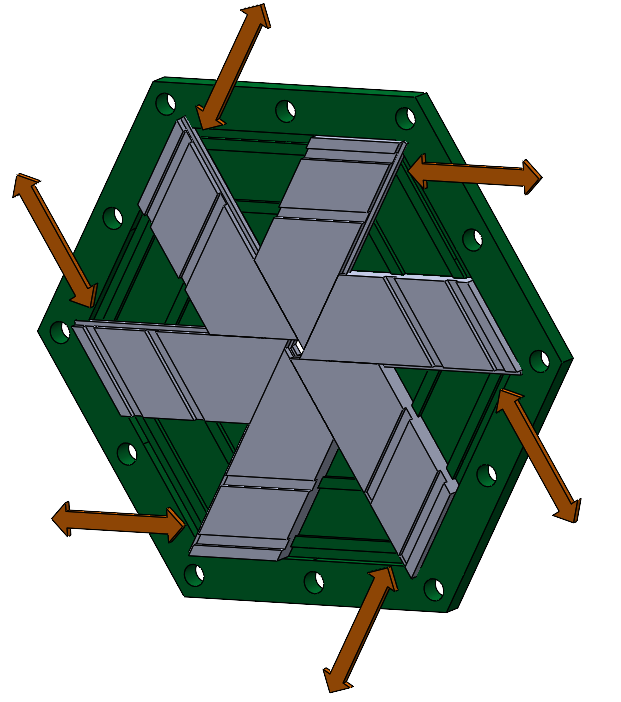
\includegraphics[width=\textwidth]{Hexagon.png}
		\captionof{figure}{Hexagonal Diaphragm}
		\label{fig:hexagon}
	\end{minipage}    
	\hfill
	\begin{minipage}[t]{0.45\textwidth}
		\centering
		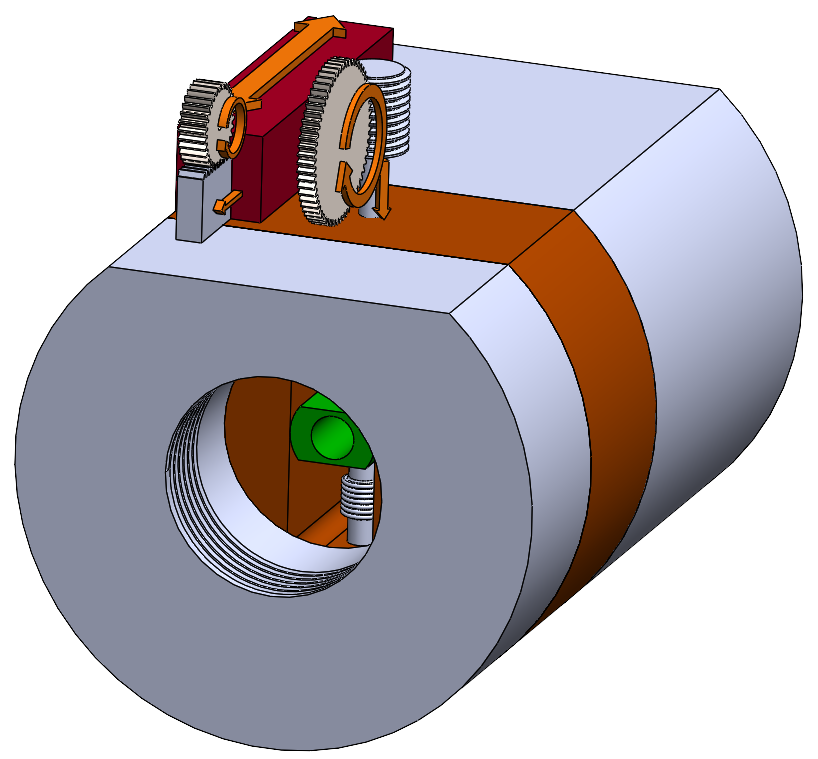
\includegraphics[width=\textwidth]{Gears.png}
		\captionof{figure}{Rack-and-Pinion Interface}
		\label{fig:gears}
	\end{minipage}    

	\vspace{1em}

	\begin{minipage}[t]{0.45\textwidth}
		\centering
		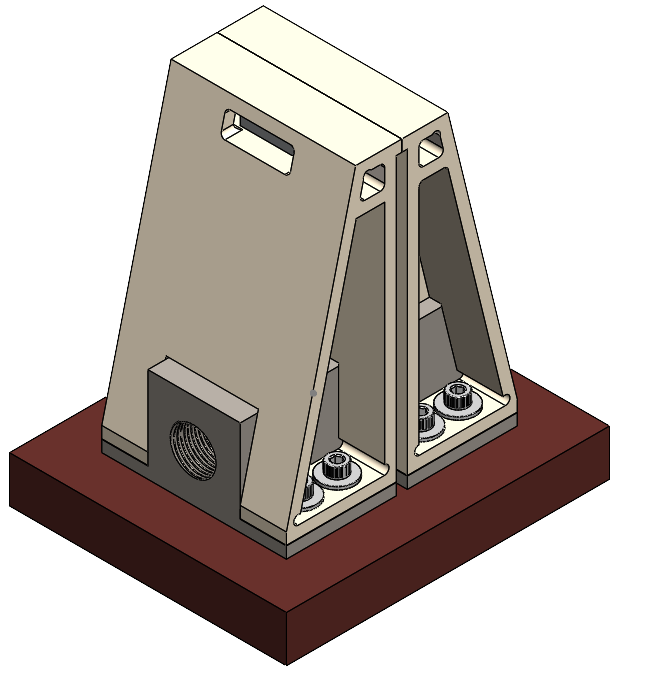
\includegraphics[width=\textwidth]{Mount_trapz.png}
		\captionof{figure}{Direct Mount, first iteration}
		\label{fig:trap_mount}
	\end{minipage}    
	\hfill
	\begin{minipage}[t]{0.45\textwidth}
		\centering
		% 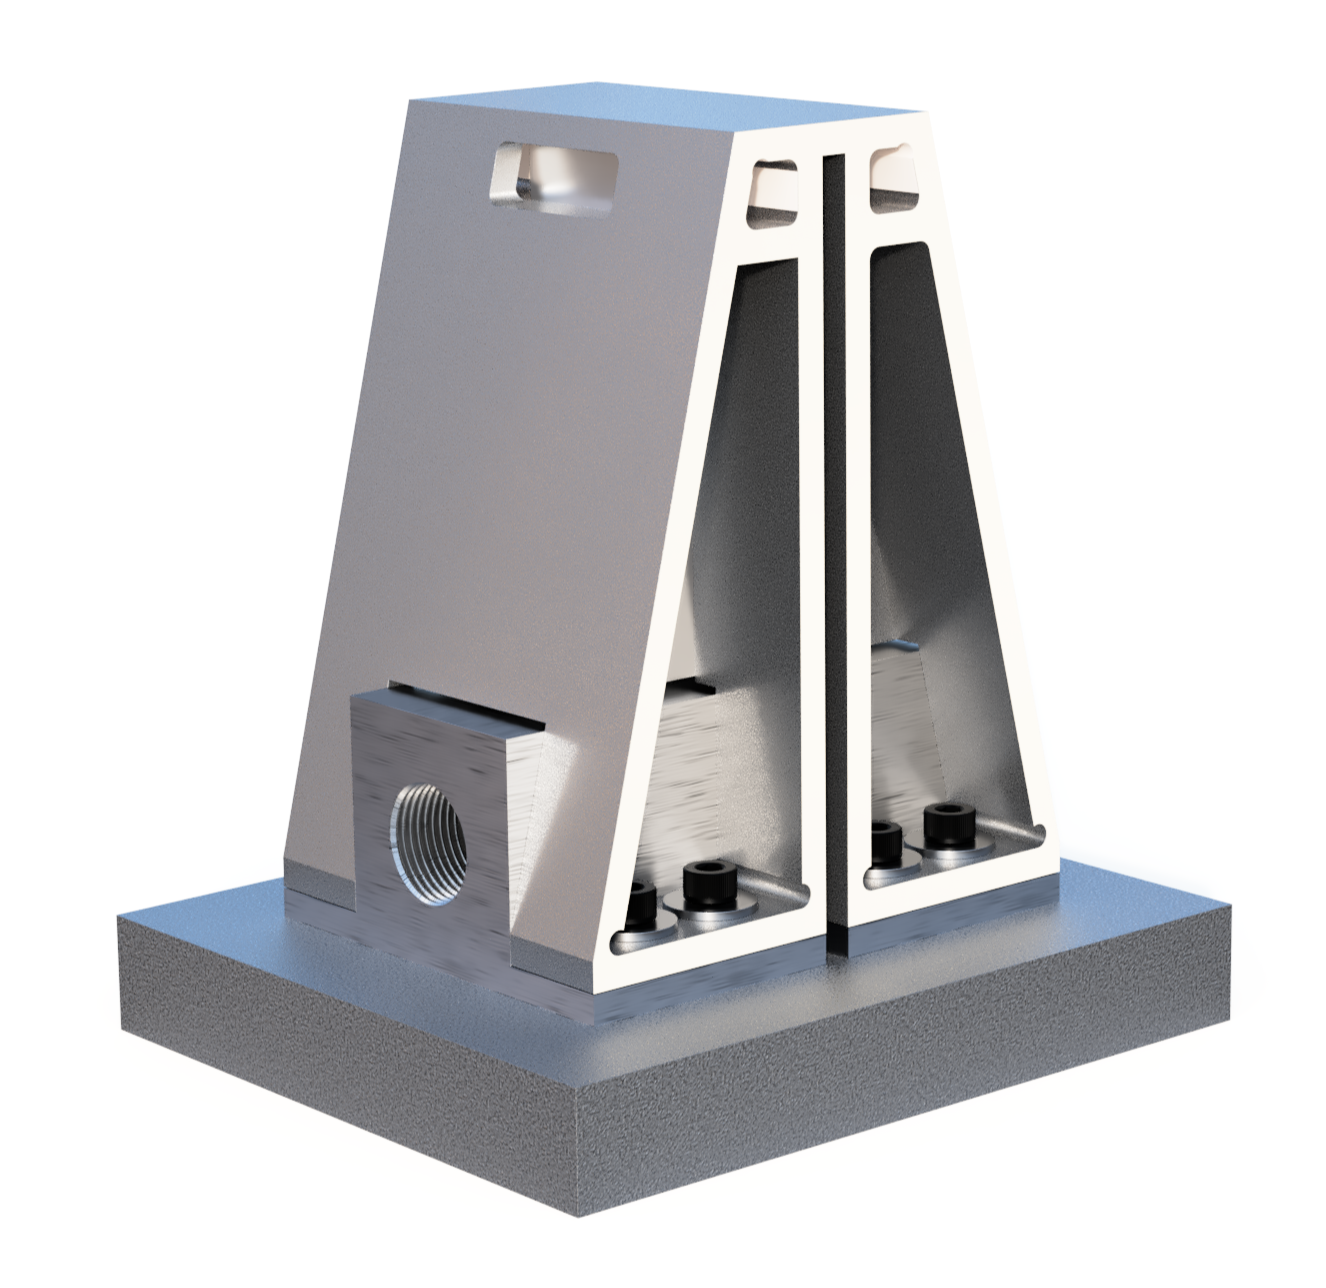
\includegraphics[width=\textwidth]{Complete_Assembly_Render.png}
		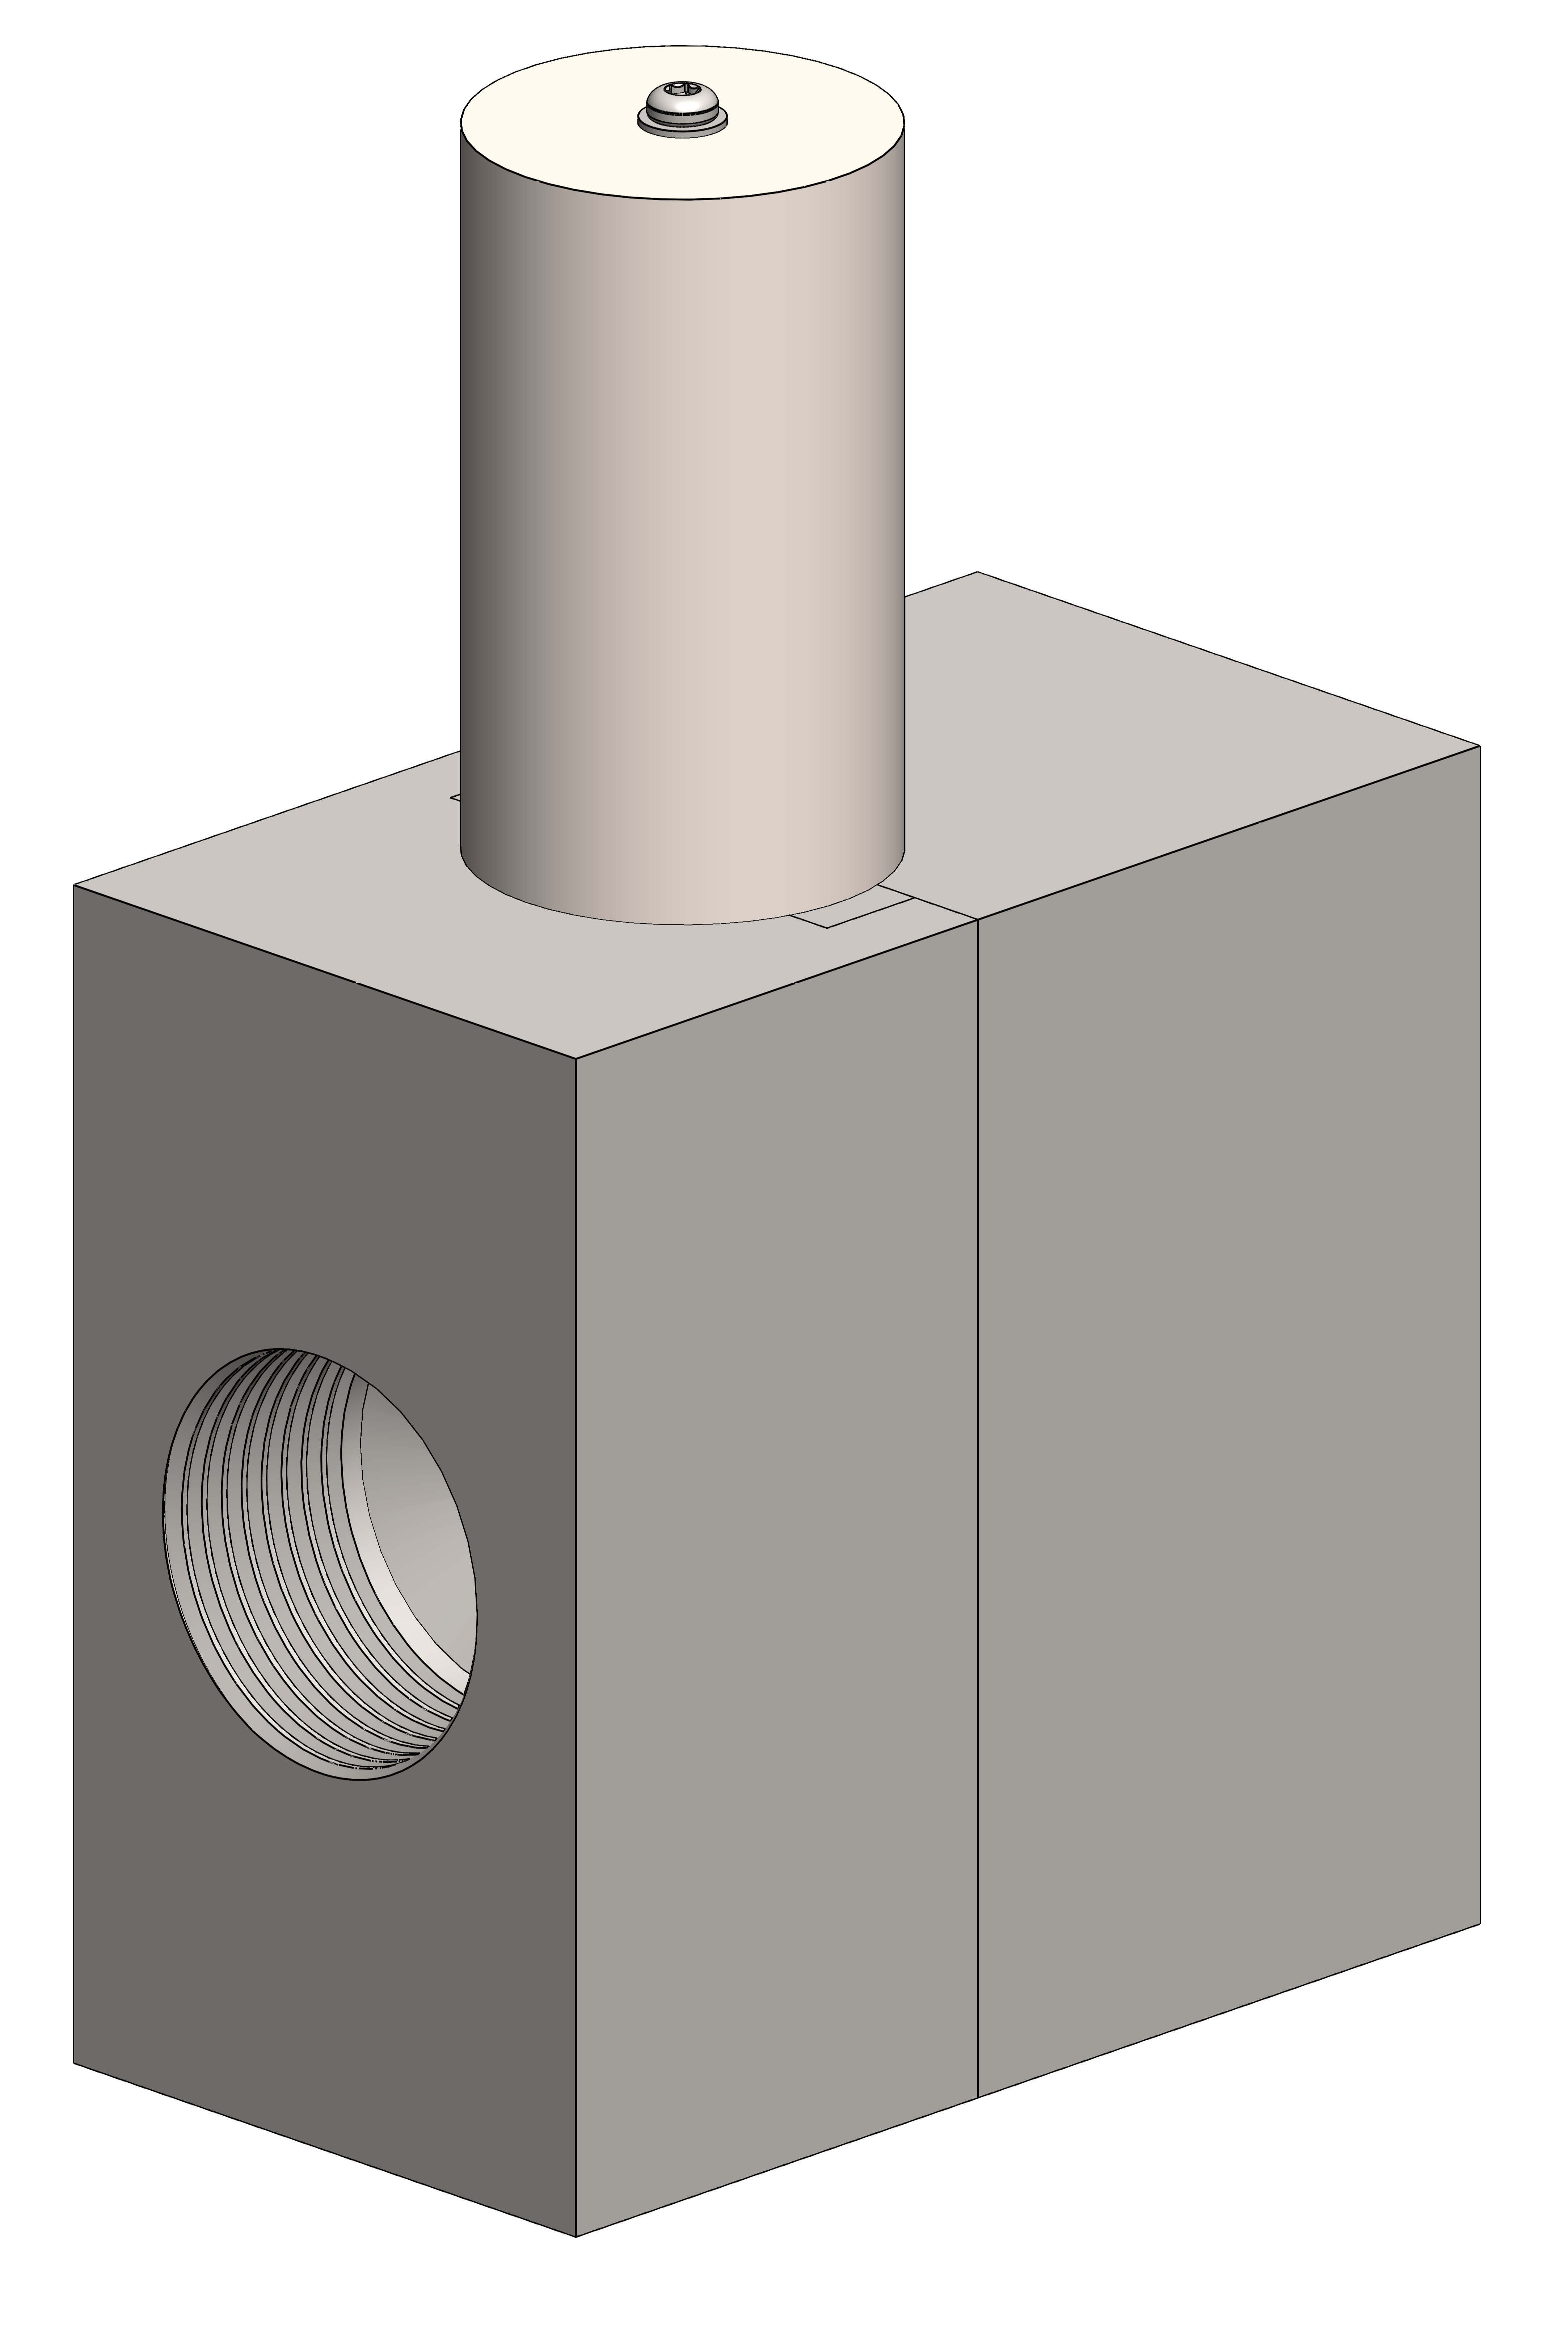
\includegraphics[width=\textwidth]{PTCD.png}
		\captionof{figure}{Cylindrical Allvar Mount}
		\label{fig:app_PTCD}
	\end{minipage}    
\end{figure}    

	\newpage
	Despite the difficulties in developing a reliable solution for this complex technical challenge, our Senior Design Project was well worth the endeavor.
	Our first exposure to real engineering design, this project will be remembered as the high point in our academic journey.

	\newpage

	\vspace*{.1\textheight}

	\begin{center}

		The authors would like to extend their sincere gratitude to
		Dr. Bradley Bon,\\
		distinguished member of the Gas Transfer Systems team\\
		at Sandia National Laboratories in Livermore, CA\\
		for his invaluable assistance in the development of this design\\[6pt]
		and to Professor Jon Schofield and Teaching Assistant Xiangpu Wang\\
		of UC Davis
		for their training and guidance.

		\vspace*{.05\textheight}

		\textit{Soli Deo Gloria,}\\
		The Noble Aggie Labs\\[24pt]

		\textit{Miguel Cuaycong}\\
		\textit{Jon Pizarro}\\
		\textit{Nicholas Metta}\\
		\textit{Isaiah Mathew}\\
		\textit{John Bodine}\\
		and \textit{Sam van der Veen}

	\end{center}

\end{appendices}

\end{document}